\documentclass{yorkThesis}

%%%%%%%%%%%%%%%%%%%%%%%%%%%%%%%%%%%%%%%%%%%%%%%%%%%%%%%%%

\usepackage[utf8]{inputenc}
\usepackage[super]{nth}

% formatting
\usepackage[super]{nth}
\usepackage{graphicx}
\usepackage{textcomp}
\usepackage{tabularx}
\usepackage{multirow}
\usepackage{placeins}
\usepackage{enumitem}
\usepackage{bm}
\usepackage{booktabs}
\usepackage{hyperref}
\usepackage{footmisc}
\usepackage{authblk}
\usepackage[tracking=true]{microtype}
\usepackage[toc,page]{appendix}
\usepackage[usenames,dvipsnames]{color}
% captioning
\usepackage{caption}
\captionsetup[figure]{labelfont=bf,textfont=md,font=footnotesize}
\captionsetup[table]{labelfont=bf,textfont=md,font=footnotesize}

%%%%%%%%%%%%%%%%%%%%%%%%%%%%%%%%%%%%%%%%%%%%%%%%%

% math
\usepackage{amsmath,amssymb,amsfonts}
\usepackage{mathtools}
\DeclarePairedDelimiter{\ceil}{\lceil}{\rceil}
\usepackage{algorithmic}
\usepackage{xfrac}
\usepackage{mathptmx}

%%%%%%%%%%%%%%%%%%%%%%%%%%%%%%%%%%%%%%%%%%%%%%%%%

% graphics
\usepackage{svg}
\usepackage{graphicx}
\usepackage{subcaption}
\usepackage{adjustbox}
\usepackage{float}
\usepackage{tikz}
\usepackage{wrapfig}
\usetikzlibrary{positioning,chains}

%%%%%%%%%%%%%%%%%%%%%%%%%%%%%%%%%%%%%%%%%%%%%%%%%%%%%%%%%

\newcommand{\lorem}{\textcolor{red}{Lorem ipsum dolor sit amet, consectetur adipiscing elit, sed do eiusmod tempor incididunt ut labore et dolore magna aliqua. Ut enim ad minim veniam, quis nostrud exercitation ullamco laboris nisi ut aliquip ex ea commodo consequat. Duis aute irure dolor in reprehenderit in voluptate velit esse cillum dolore eu fugiat nulla pariatur. Excepteur sint occaecat cupidatat non proident, sunt in culpa qui officia deserunt mollit anim id est laborum.\\}}

%%%%%%%%%%%%%%%%%%%%%%%%%%%%%%%%%%%%%%%%%%%%%%%%%%%%%%%%%

\title{
{A Methodology for Approximating Motivation-Related Latent States in Large Scale Scenarios}\\
{\small And its Application to Engagement Prediction in a Videogames Setting}\\
{\Large PhD}\\
{\large University of York}\\
{\large Department of Computer Science}\\

}
\author{Valerio Bonometti}

%%%%%%%%%%%%%%%%%%%%%%%%%%%%%%%%%%%%%%%%%%%%%%%%%%%%%%%%%

\begin{document}

\maketitle

\chapter*{Abstract}
\label{abstract}
Motivation is a fundamental psychological process guiding our everyday behaviour. For doing so, it heavily relies on the ability to attribute relevance to potentially rewarding objects and actions (i.e. incentives). However, despite its importance, quantifying the saliency that an individual might attribute to an object is not an easy task, especially if done in naturalistic contexts. In this view, this thesis aims to outline a methodology for approximating the ammount of attributed incentive salience in situations where large volumes of behavioural data are available but no experimental control is possible. Leveraging knowledge derived from theoretical and computational accounts of incentive salience attribution we designed an Artificial Neural Network (ANN) tasked to infer a latent representation able to predict duration and intensity of future interactions between individuals and a series of video games. We found video games to be the ideal context for developing such methodology due to their reliance on reward mechanics and their ability to provide ecologically robust behavioural measures at scale. We tested our methodology on a series of large-scale ($N> 10^6$) longitudinal datasets evaluating the ability of the generated latent representation to approximate some functional properties of attributed incentive salience. The present work opens with an overview of the concept of motivation and its interconnection with engagement in a video-game setting. It proceeds by formulating the theoretical and computation foundations on which our methodology is built upon. It then describes the iterative process of model building, evaluation and expansion underlying the implementation of our methodology. It continues by analyzing the latent representation generated by the ANN and comparing its functional characteristics with those of attributed incentive salience. The manuscript ends with a general overview of the potential applications of our methodology with a particular focus on the area of automated engagement quantification in videogames settings.

\chapter*{Dedication}
\label{dedication}
\lorem

\chapter*{Declaration}
\label{declaration}
I declare that this thesis is a presentation of original work and I am the sole author. This work has not previously been presented for an award at this, or any other, University. All sources are acknowledged as References. The work presented in this thesis is the result of a partnership between University of York and Square Enix Ltd. It was supported by the EPSRC Centre for Doctoral Training in Intelligent Games \& Games Intelligence (IGGI) through grant [EP/L015846/1]. All data employed in this work were obtained and processed in compliance with the European Union's General Data Protection Regulation \cite{EUdataregulations2018} and Square Enix Ltd. data protection policies. Chapter \ref{chapter_theory_modelling} is based on the work carried out in \cite{bonometti2020theory, bonometti2021approximating}. Chapter \ref{chapter_implementation_testing} is based on the work carried out in \cite{bonometti2019modelling, bonometti2020theory, bonometti2021approximating}. Chapter \ref{chapter_repr_anal} is based on the work carried out in \cite{bonometti2021approximating}.

\chapter*{Acknowledgements}
\label{acknowledgements}
This work was supported by the EPSRC Centre for Doctoral Training in Intelligent Games \& Games Intelligence (IGGI) through grant [EP/L015846/1]. The partner company Square Enix Ltd. provided all the data used for the development of this work.

\chapter*{General Introduction}
\label{chapter_general_intro}
When we see a professional athlete competing at an event we often find ourself thinking "how much work they must have done to reach such level of performance". Similarly we might be surprised discovering the effort miners were putting in finding even small ammount of gold nuggets during the \nth{19} century gold rush. Looking at something closer to our everyday experience, we widen our eyes noticing how many hours we sank watching the latest tv-series or playing our favourite videogames. But what do all these activities have in common? They are very different from each other but nevertheless able to elicit prolonged and vigorous behavioural responses. Indeed, it appears that human beings are capable of remarkable feats when trying to achieve goals that lead to positive and pleasurable outcomes for them. From psychological point of view, we say that in all those instances a common set of cognitive and affective processes, which go under the umbrella of "motivation", are involved in the generation of goal-directed behaviour. This implies that knowing the motivational state of an individual, during a particular activity, puts us in a favourable position for interpreting their behaviour and predicting its future intensity. Within this general framework lies the aim of this thesis, with the current work we attempted to develop a methodology for deriving an approximate quantification of the motivational drive of individuals in situations where large volumes of observational data are present but no direct contact is possible.

\section*{Thesis Outline}
The work carried out for this thesis, although originated for addressing a series of academic challenges (e.g. inferring the motivational states of individuals from large scale behavioural data) it has been developed completely within an industrial setting. It is therefore the product of two separate although complementary tensions: the academic need to advance knowledge and tackle problems which have not yet found a solution and the constrains imposed by the industry to develop actionable tools.

\paragraph*{Academic Outline}
\label{academic_outline}
From an academic point view we found that despite there has been noticeable interest in the estimation of the internal states generated by various psychological processes (e.g. motor control \cite{gallego2017neural}, memory \cite{derdikman2011manifold, nieh2021geometry}, visual \cite{seung2000manifold, ganmor2015thesaurus} and olfactory \cite{stopfer2003intensity} perception), less work has taken into consideration the construct of motivation \cite{mcclure2003computational, zhang2009neural}. In addition, most of efforts in this area of research have focused on data generated in laboratory or simulation settings \cite{eyjolfsdottir2016learning, song2017reward, merel2019deep,calhoun2019unsupervised, seung2000manifold, pang2016dimensionality, luxem2020identifying, pereira2020quantifying, mccullough2021unsupervised, shi2021learning} leaving the estimation of internal states from observational data a somewhat under-explored venue, with a major focus on animal behaviour and a marked preference for completely data-driven approaches \cite{luxem2020identifying,pereira2020quantifying, mccullough2021unsupervised}. In this view our approach has been to bridge the gap between theoretical and computational account of motivation and data driven approaches for its inference. With the aim to design, develop and validate a methodology for approximating the motivational states of individuals solely from large volumes of behavioural data acquired in naturalistic settings. 

\paragraph*{Industrial Outline}
\label{industrial_outline}
One factor limiting the inference of psychological states in ecologically plausible settings has been the challenge to acquire sufficient ammount of data in a relatively unbiased manner. This issue has been partially attenuated by the, now not-so-recent, tendency to acquire behavioural data through telemetries \cite{el2016game, drachen2015behavioral}. A practice, that has seen an incredible explosion in industrial settings to the point of requiring international regulatory interventions \cite{EUdataregulations2018}. In this view, a collaboration between academia and industry seems a promising venue for tackling some of the problems mentioned in paragraph \ref{academic_outline}. That said, industries are often laser-focused on delivering practical and actionable tools serving the ultimate purpose of improving their operations. In this view, given our strong partnership with the videogame industry, our approach has been to highlight the strong connection between motivation and the more actionable construct of engagement. While doing so, we also showed how the methodology developed in this thesis has not just direct and practical implication for automated engagement prediction and quantification, but is also able to overcome some of the limitation of current state of the art approaches. 
\\
\\
The thesis will open with an overview on the literature on motivation and engagement highlighting how the latter can be seen as a behavioural derivative of the motivational state of an individual. Next, it will illustrate various approaches for characterizing and quantifying both engagement and motivation highlighting their strengths and weaknesses. The chapter closes with a review of data-driven approaches for inferring the motivational state of individuals and predicting engagement in large scale scenarios. Chapter two attempts to illustrate how theoretical and computational model derived from the filed of behavioural neuroscience can be leveraged for designing approaches aimed to estimate the latent states produced by motivation. It opens introducing the idea that latent states produced by motivational processes can be represented as a manifold on which observable behaviour resides. It continues illustrating a computational model of incentive salience, a particular theoretical account of reward-driven motivation, and how its underlying principles can be used for defining the architecture of an artificial neural network (ANNs). The chapter closes by proposing the idea that the ammount of motivational drive that an individual exhibits can be approximated by the manifold structured inferred by an ANN tasked to solved a supervised learning problem. Chapter three focuses on translating the theoretical insights derived from chapter 2 in an actual implementation. The chapter attempts to achieve the implementation of the optimal model defined in chapter two by iterative model building. Starting from a basic formulation, additional components are added during three separate cycles of model specification, validation and expansion. Chapter four delve into the analysis of the representations generated by the models defined in chapter three, focusing on comparing their functional characteristics with those of attributed incentive salience. Chapter five shows a potential application of the work presented so far in the context of automated engagement prediction and qualification in large scale scenarios. The thesis closes with a summary of the findings illustrated in each chapter, their limitation as well as recommendations and venues for future research.




\tableofcontents

%%%%%%%%%%%%%%%%%%%%%%%%%%%%%%%%%%%%%%%%%%%%%%%%%%%%%%%%%

\chapter{Motivation and Engagement}
\label{chapter_lit_review}
\section{Introduction}
\label{motivation_engagement_introduction}
In this chapter we will discuss the concept of motivation and how it can be used to describe the interactions that individuals have with particular objects or activities. We will first provide a general introduction to the construct of motivation followed by a short historical review of theories of reward-driven motivation. We will then focus on how these led to the incentive salience hypothesis formulated by Berridge and Robinson \cite{berridge1998role}. While acknowledging the contribution of other theories in the definition of motivation (and reward-driven motivation in particular) this thesis will mostly focus on the areas of behavioural and affective neuroscience and make use of the framework provided by Berridge and Robinson \cite{berridge1998role}. The reason behind this choice lies in the fact that we found incentive salience to be more specific to motivation and most importantly to have a more robust and clear connection to behaviour. The chapter will then provide a description of the concept of engagement highlighting how this can be seen as a behavioural derivation of the latent states generated by motivational processes. We will contextualise engagement in the context of videogames presenting a quick overview of the various taxonomies describing how different videogames structural characteristics fuel the motivational processes underlying the engagement behaviour. The chapter closes presenting various approaches for measuring, describing and predicting both engagement and motivation, with a particular focus on the challenges derived by their application in large scale scenarios.

\section{Motivation as a Reward-Driven Process}
\label{motivation}
The construct of motivation is a key concept for understanding why individuals seek out specific objects or experiences at particular times and why they react in particular ways when encountering objects considered of particular relevance \cite{berridge2004motivation}. In this view motivation can be defined as the process leading to the modulation and reiteration of goal directed behaviours that once reached exerts positive effects on the individual \cite{simpson2016behavioral}. A formal definition of motivation should encompass both the behavioural and the underlying psychobiological level. We will focus first on behavioural aspects of the process and outline in the following sections a theoretical account of motivation which also covers the psychobiological level. As we mentioned before, motivation describes why individuals react in particular ways when encountering objects regarded of high relevance and why they approach those objects at particular times \cite{berridge2004motivation}. These type of objects are said to possess "rewarding properties", which can be defined as the positive value ascribed to an object, a behavioral act or an internal physical state as the result of an active process of the mind and the brain \cite{schultz1997neural,berridge2008affective}. Importantly, motivation is not just driven by the fulfilment of fundamental needs like nutrition or reproduction (so-called "primary reward objects" \cite{schultz2000reward}) or the avoidance of negative consequences like physical pain. It also extends to those volitional objects and activities which do not appear to be necessary for the survival of the individual (i.e. "secondary reward objects" \cite{berridge2008affective,sescousse2013processing}). For those activities the expectation of the amount of reward received is learned over time and may vary significantly between individuals \cite{berridge2008affective,simpson2016behavioral}.In spite of this, it would be inefficient to have dedicated and specialized motivational systems for every combination of individuals and objects (e.g. an individual's motivation for playing sport or eating food). Instead, we can think of motivation as a single overarching entity that controls the interaction between individuals and objects in an agnostic manner \cite{simpson2016behavioral}. An analogy may be drawn with the geometric concept of a vector. Looking at Figure \ref{fig: vect_mot} we can imagine the focus on a specific object being represented by the angle of the vector while its length is the intensity of the motivational process (or the amount of motivated behaviour) \cite{simpson2016behavioral}. This, can be thought as a dynamic quantity defined by the state of the individual and the rewarding properties of the object \cite{toates1994comparing,berridge2004motivation,zhang2009neural}.
\begin{figure}[h]
  \begin{center}
    \begin{adjustbox}{width=0.5\columnwidth}
        \tikzset{every picture/.style={line width=0.75pt}} %set default line width to 0.75pt        
            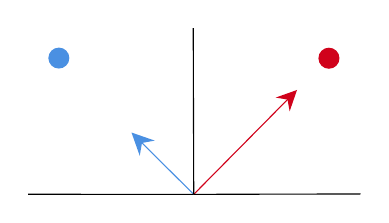
\begin{tikzpicture}[x=0.75pt,y=0.75pt,yscale=-1,xscale=1]
            %uncomment if require: \path (0,300); %set diagram left start at 0, and has height of 300
            
            %Straight Lines [id:da17586827840068286] 
            \draw [color={rgb, 255:red, 208; green, 2; blue, 27 }  ,draw opacity=1 ]   (190.24,200.32) -- (237.89,152.16) ;
            \draw [shift={(240,150.03)}, rotate = 494.69] [fill={rgb, 255:red, 208; green, 2; blue, 27 }  ,fill opacity=1 ][line width=0.08]  [draw opacity=0] (9.82,-4.72) -- (0,0) -- (9.82,4.72) -- (6.52,0) -- cycle    ;
            %Straight Lines [id:da23704064540856618] 
            \draw [color={rgb, 255:red, 74; green, 144; blue, 226 }  ,draw opacity=1 ]   (190.24,200.32) -- (162.38,172.64) ;
            \draw [shift={(160.25,170.53)}, rotate = 404.81] [fill={rgb, 255:red, 74; green, 144; blue, 226 }  ,fill opacity=1 ][line width=0.08]  [draw opacity=0] (10.72,-5.15) -- (0,0) -- (10.72,5.15) -- (7.12,0) -- cycle    ;
            %Shape: Circle [id:dp3839733612485111] 
            \draw  [color={rgb, 255:red, 208; green, 2; blue, 27 }  ,draw opacity=1 ][fill={rgb, 255:red, 208; green, 2; blue, 27 }  ,fill opacity=1 ] (250.58,134.73) .. controls (250.58,132.08) and (252.73,129.93) .. (255.38,129.93) .. controls (258.03,129.93) and (260.18,132.08) .. (260.18,134.73) .. controls (260.18,137.38) and (258.03,139.53) .. (255.38,139.53) .. controls (252.73,139.53) and (250.58,137.38) .. (250.58,134.73) -- cycle ;
            %Shape: Circle [id:dp009447430116501954] 
            \draw  [color={rgb, 255:red, 74; green, 144; blue, 226 }  ,draw opacity=1 ][fill={rgb, 255:red, 74; green, 144; blue, 226 }  ,fill opacity=1 ] (120.47,134.66) .. controls (120.47,132.02) and (122.61,129.88) .. (125.25,129.88) .. controls (127.89,129.88) and (130.03,132.02) .. (130.03,134.66) .. controls (130.03,137.29) and (127.89,139.43) .. (125.25,139.43) .. controls (122.61,139.43) and (120.47,137.29) .. (120.47,134.66) -- cycle ;
            %Straight Lines [id:da5714219654763008] 
            \draw    (190,120.28) -- (190.24,200.32) ;
            %Straight Lines [id:da22247567054966455] 
            \draw    (110.5,200.28) -- (190.24,200.32) ;
            %Straight Lines [id:da4124676757039665] 
            \draw    (270.64,200.12) -- (190.24,200.32) ;
            
            
            
            
            \end{tikzpicture}
    \end{adjustbox}
  \end{center}
\caption{\textbf{Motivation as a vector}. Blue and red dots represent two objects with different characteristics while the two arrows illustrate the hypothetical motivational propensity of an individual (or two individuals) towards them. The black segments delineate the space created by the combination of the objects' characteristics and the motivational propensity of the individuals. Here the red object has the potential to generate more behaviour than the blue object possibly as a result of its characteristics and those of the individual interacting with it.}
\label{fig: vect_mot}
\end{figure}
Summarizing we can say that from a motivational point of view, the behaviour of an individual is driven by the expectancy of pleasurable outcomes derived by the goal the behaviour is aiming to reach \cite{berridge2004motivation}. Therefore, if motivation acts as a single overarching process, we expect it to hold predictive and explanatory power over goal directed behaviour seamlessly across a heterogeneous range of situations and individuals. Motivational theories based on the concepts of reward and incentive are promising candidates for this because, relying on consistent and plausible psychobiological bases, they tend to operate abstracting from the nature of the individuals and the objects. \cite{ikemoto1999role,berridge1998role,salamone2002motivational,berridge2004motivation,armony2013cambridge,corbit2015learning}.

\subsection{An Historical View on Reward-driven Motivation}
\label{motivation_hist}
Introducing the processes of classical and operant conditioning is an essential step for describing theories of reward-driven motivation, in particular if we are interested in their behavioural correlates. Both constructs heavily rely on the general concepts of reinforcer and reinforcement process. Simply put, reinforcers are those objects or actions that have the ability to alter the likelyhood of appearance of specific behaviours \cite{kling1971woodworth,skinner1953science,squire2012fundamental}. A reinforcement process instead define the learning mechanisms by which a specific behaviour becomes, over time, more or less probable conditional on the presence of particular reinforcers \cite{kling1971woodworth}. In this view we can think of classical and operant conditioning as two complementary oprationalizations of the reinforcement process. Classical conditioning describes the learning process in which, independently from the activity of an individual, the repeated pairing of two objects will cause one to acquire the eliciting properties of the other \cite{squire2012fundamental}. In other words, the repeated pairing of a neutral object with reinforcing consequences will imbue the first with reinforcement properties making it a reinforcer. Operant conditioning on the other hand, extends the concept of classical conditioning introducing the agency of the individual \cite{skinner1953science}. The frequency of behaviour produced by an individual tends to increase when precise consequences are associated to it \cite{skinner1953science}. In this view, an operant is formalized as a goal directed behaviour while all the elements reinforcing the re-iteration of this behaviour are called reinforcers \cite{skinner1953science}. The learning process here results from the relationship between a behaviour and its consequences, therefore the probability of behaviour to take place is related to its capability to generate reinforcer \cite{kling1971woodworth}. Both classical and operant conditioning are of course very simplistic accounts of human behaviour, but nevertheless able to succinctly illustrate a fundamental process by which most (if not all) individuals are able to learn and leverage the association between actions and the positive (i.e. rewarding) consequences associated to them. In this regard, it is not surprising that many theories of reward-driven motivation stem directly from these two constructs. For example, in its work Bolles \cite{bolles1972reinforcement} suggested that individuals were motivated by the "expectations of incentive outcomes". These expectations are formed through a learning process where an association between actions and potential pleasurable outcomes is created \cite{bolles1972reinforcement,berridge2004motivation}. Expanding on this idea, Bindra suggested that the learning process does not just generate pleasure expectations in response to specific behaviours but it also allows individuals to perceive the behaviours themselves as a source of hedonic reward \cite{bindra1978adaptive,berridge2004motivation}.
This introduces the concept of learning through reinforcement: an object and the behaviours associated to it become relevant and salient for an individual as a consequence of learning its incentive properties \cite{berridge2004motivation}. A third theoretical formulation by Toates \cite{toates1994comparing}, asserted that the magnitude of the perceived incentives introduced by both Bolles and Bindra is modulated by the internal states of the individual \cite{toates1994comparing,berridge2004motivation}. In other words, the incentive expectations (and consequently the associated motivated behaviours) learned by an individual can change over time depending on the individual's internal state. Until now we have mainly used the terms reinforces and incentives for identifying objects able to drive and shape behaviour, but when it comes to define effective reinforces, it is not just a matter of merely pairing a behaviour with a stimulus but the stimulus itself has to have particular properties. In this view, stimuli able to generate pleasurable feelings in the individual are the best candidates for being effective reinforces, they are said having ‘rewarding properties’. But what is, and how can be defined the reward? The reward is a process generated in response to a stimulus making it desirable for its capacity to generate pleasurable responses. In this view, for being able to generate rewarding response, a stimulus needs two fundamental properties: it has to be wanted (i.e. it acquires the capacity to become desirable) and liked (i.e. it has to be able to generate pleasure in the individual) \cite{berridge2009dissecting}. But how a particular object acquires these properties? This is mostly carried out by the same learning processes mentioned in section \ref{motivation_hist}. The repeated pairing of a stimulus with the (positive) consequences it exerts on the individual will imbue the first with so called rewarding properties. Moreover, through operant conditioning  not just the stimulus itself but also the connected instrumental behaviour will likely acquire the same rewarding properties \cite{berridge2009dissecting}. As anticipated in section \ref{motivation}, a useful distinction that can be made is between objects having primary and secondary reward properties. Objects linked with essential evolutionary needs (i.e. satisfaction of homeostatic needs) are on a fast track for becoming reinforcers, their rewarding properties don’t have to be learned but are, up to a certain extent, intrinsic to them \cite{sescousse2013processing}. Classical examples of primary rewards are food, mating-related activities and drug of abuse \cite{berridge2004motivation, simpson2016behavioral}. On the other hand, objects with so called secondary rewarding properties don’t hold an innate capacity to generate pleasurable experiences, this capacity is acquired by means of the same learning mechanisms we've just presented \cite{sescousse2013processing}. 

\subsection{The Incentive Salience Theory of Motivation}
\label{incentive_salience}
The approaches proposed by Bolles, Bindra and Toates,  provide an account of reward-based motivation but they assume that there is no distinction between the affective dimension of an incentive (i.e. how pleasurable it is) and the purely motivational aspect of it (i.e. how much goal directed behaviour it can produce) \cite{bindra1978adaptive,toates1994comparing}. Expanding on this, Berridge and Robinson proposed that the motivational process controlling the interaction between individuals and objects might not be a unitary mechanism but rather a composite process having specific and dissociable components which rely on specialized neurobiological mechanisms, namely: \emph{liking}, \emph{wanting} and \emph{learning} \cite{berridge1998role,berridge2009dissecting,smith2011disentangling}.

\paragraph*{Liking}
\label{liking}
The \emph{liking} component describes the pleasure expected by an individual when interacting with an object \cite{berridge2009dissecting}. It is responsible for the hedonic quality of an experience and acts as a signal indicating that interacting again with that object might be beneficial. Despite the fact that \emph{liking} plays an important role in the incentive salience hypothesis of motivation it is difficult to measure it outside controlled laboratory environments \cite{berridge1998role} and it will not form a central theme of this thesis. Instead, we will focus on the "wanting" and "learning" components.

\paragraph*{Wanting}
\label{wanting}
The \emph{wanting} component, or "incentive salience", has the function of generating and holding latent representation of objects and behavioural acts and of attributing value to them through learning mechanisms. These "valued representations" can then be used by action selection systems in order to make certain behaviours more likely \cite{ikemoto1996dissociations,berridge1998role,mcclure2003computational,berridge2004motivation}. As a consequence of this, when an object is attributed with incentive salience it will more likely draw the subject's attention and become the focus of goal directed behaviours \cite{berridge2004motivation}. Interestingly, \emph{wanting} seems to be more than a simple form of value-caching but rather a dynamic process in constant change \cite{robinson1993neural,zhang2009neural,tindell2009dynamic,berridge2012prediction}. This is because the saliency of an object depends both on its attributed value but also on the state of the individual interacting with it. A change in the individual's internal state can dampen, magnify or even revert the amount of attributed salience. \cite{robinson1993neural,zhang2009neural,tindell2009dynamic,berridge2012prediction}. It is important to note that \emph{wanting} is not the hedonic expectation associated to an object, (which is designated by \emph{liking}), but rather the process promoting the approach towards an object and the interaction with it \cite{berridge2009dissecting,robinson2015roles}. Despite the fact that \emph{liking} and \emph{wanting} are often correlated (i.e. I want what I like and vice versa) they can occasionally be triggered separately: addictive behaviours for instance are a notable example of \emph{wanting} without \emph{liking} \cite{robinson1993neural}. The functional dissociation between these two components is linked to differences in the underlying neurobiological substrate \cite{berridge2009dissecting,smith2011disentangling}. Neurotransmitters and brain areas responsible for \emph{wanting} appear to be more numerous, diverse and easily activated than those for \emph{liking} \cite{berridge2009dissecting,robinson2015roles}. As a consequence, increased incentive salience can be obtained by raising dopamine levels in many portion of the striatum without the need for the synchronized activity in other areas \cite{berridge2009dissecting,smith2011disentangling,meyer2015motivational}. This implies that the \emph{wanting} component tends to produce more robust behavioural indicators in the form of increased amount and frequency of interactions between an individual and an object \cite{berridge1998role}, which makes it a promising candidate for behavioural studies in conditions where strict experimental control is not possible.

\paragraph*{Learning}
\label{learning}
The last component in the formulation proposed by Berridge and Robinson \cite{berridge1998role,berridge2004motivation} consists of mechanisms that provide an individual with the capability to predict, based on past experiences, the occurrence of future pleasurable outcomes (i.e. \emph{liking} reactions) when interacting with specific objects. These are similar to the learning processes illustrated in section \ref{motivation_hist} and have a twofold function. These mechanisms allow the attribution and change of incentive salience properties to previously \emph{liked} objects (e.g. primary reward objects) but they also enable subjects to learn the hedonic value of initially neutral stimuli (e.g. secondary reward objects). The \emph{learning} mechanism is based on classical conditioning: through repeated interactions with an object an individual will learn its hedonic properties and consequently attribute incentive salience to it \cite{berridge2004motivation,berridge2009dissecting}. This process is driven by mechanisms similar to those of reward-prediction error: learning is driven by spikes in dopaminergic activity generated by a mismatch between expected and experienced rewards. \cite{schultz1997neural,schultz2000multiple,flagel2011selective}.

\section{Engagement as a Derivative of Motivation}
\label{engagement}
We will now momentarily diverge from our discussion on motivation for introducing the construct of engagement. The reason for this brief detour lies in the fact that presenting the construct of engagement allows us to better understand the practical implication that motivational processes have in our everyday life. Despite engagement has applications in a wide range of contexts, we think it is better understood when framed within a specific class of activities. In this view, given the background from which this work has arisen, we will focus on the area of videogames but we will make evident how, by framing engagement as a byproduct of motivational processes, we can easily generalize it to other type of activities.

\subsection{Theories of Engagement}
\label{factors_engagement}
Playing games has always been present in human history as an occupation aiming to entertain and relax \cite{connolly2012systematic}, it can be defined as a free-time activity with spatial and temporal boundaries able to intensely absorb who is involved in it \cite{connolly2012systematic}. A special case of the broader group of games are those delivered and experienced in a digital format (i.e. videogames) which in the last decades has been substituting more traditional playful activities \cite{boyle2012engagement,connolly2012systematic}. This phenomenon has been reflected both in terms of number of people involved in playing videogames as well as in the amount of time spent engaging in this activity \cite{boyle2012engagement}. One of the main reasons for this explosive phenomenon is the fact that videogames seems to be perfect medium for delivering pleasurable experiences \cite{boyle2012engagement}, consequently holding a strong potential to engage and retain users involved in the playing activity. Various attempt has been made to understand engagement in videogames, both as unitary process and at the level of factors driving and influencing it \cite{boyle2012engagement}. The literature on the subject is abundant although extremely heterogeneous \cite{boyle2012engagement}. A clear example of this heterogeneity is the definition of engagement provided by O'Brien et al. \cite{o2008user}:
\textit{"...a quality of user experiences with technology that is characterized by challenge, aesthetic and sensory appeal, feedback, novelty, interactivity, perceived control and time, awareness, motivation, interest and affect..."}
this definition, although providing a good holistic description, makes it exceptionally hard to clearly define a unitary framework for defining engagement let alone specifying its mechanistic aspects. This lack of theoretical formalism is reflected in most (if not all) accounts of engagement and, to a certain extent, inevitable given the breadth of the behavioural, cognitive and affective aspects that the construct tries to cover. Nevertheless, inspecting some of the most prominent theories of engagement we can individuate some common themes useful for composing a unifed framework.

\paragraph*{Flow} This is a classical construct often occurring in the videogame literature for explaining the phenomenon of engagement. Developed by Csikszentmihalyi \cite{csikszentmihalyi2014toward}, the construct of flow prescribes that when an individual is absorbed in an activity perceived as valuable they will experience a rewarding state of optimal pleasure constituting the fuel for of engagement process \cite{boyle2012engagement}. In this view, conditio sine qua non for the flow state to arise is a balanced combination of the individual’ state level and the characteristics of the interaction in which they are involved \cite{boyle2012engagement,csikszentmihalyi2014toward}. Despite offering an interesting point of view, the concept of flow as a framework for explaining engagement might be prone to the fallacy of circular reasoning: is an individual engaged in a specific activity because this provides the optimal flow experience or this last one is a bi-product of being engaged in the activity itself? 

\paragraph*{Immersion} This construct is closely connected to that of flow but specifically concerned with the psychological experience of engaging with a computer game \cite{jennett2008measuring}. Immersion tries to describe the experience of engaging in a specific moment in time with a videogame  rather than posing itself as a factor influencing or driving engagement \cite{jennett2008measuring}. According to Jennet et al. \cite{jennett2008measuring}, as a result of a good gaming experience, an individual might loose track of time and space and will experience a sense of being completely "immersed" in the playing activity.

\paragraph*{Uses and gratification} This theory states that the consumption of media is a way for individuals to satisfy the need for gratification (i.e. reward). The gratification-seeking behaviour is then driven and characterized by the nature of the underlying motive generating them (e.g. my need to connect with other people drives my social-media consumption) \cite{lucas2004sex}. Again, according to this theory, individuals are not passive bystanders but will actively interact with a specific media object based on its ability to meet the individual's underlying motivational drive. Uses and gratification theory introduce two important concepts: first that individuals engage in a spontaneous activity (i.e. media object interaction) in search of some form of gratification and second that this interaction is not passive but rather an active process.

\subsubsection{The Engagement Process Model}
\label{eng_proc_model}
We will focus now on an relatively atypical formalization of the construct of engagement, the engagement process model formulated by O'Brien and colleagues \cite{o2008user}. This framework, instead of presenting engagement as a static entity proposes the idea that it is better understood as a dynamic process \cite{o2008user}. O'Brien et al. avoid to give an exact definition of engagement but rather describe it as a process with distinct phases each one possessing peculiar attributes \cite{o2008user}:
\begin{figure}[h]
\begin{center}
\begin{adjustbox}{width=\textwidth}

% Gradient Info
  
\tikzset {_2yn49zl61/.code = {\pgfsetadditionalshadetransform{ \pgftransformshift{\pgfpoint{0 bp } { 0 bp }  }  \pgftransformrotate{0 }  \pgftransformscale{2 }  }}}
\pgfdeclarehorizontalshading{_f0h1xn2np}{150bp}{rgb(0bp)=(0.88,0.88,0.88);
rgb(37.5bp)=(0.88,0.88,0.88);
rgb(49.53571319580078bp)=(0.88,0.88,0.88);
rgb(62.5bp)=(1,0,0);
rgb(100bp)=(1,0,0)}
\tikzset{_ao557rzfs/.code = {\pgfsetadditionalshadetransform{\pgftransformshift{\pgfpoint{0 bp } { 0 bp }  }  \pgftransformrotate{0 }  \pgftransformscale{2 } }}}
\pgfdeclarehorizontalshading{_b1qqyoil7} {150bp} {color(0bp)=(transparent!61);
color(37.5bp)=(transparent!61);
color(49.53571319580078bp)=(transparent!75);
color(62.5bp)=(transparent!75);
color(100bp)=(transparent!75) } 
\pgfdeclarefading{_gj5ns3oqm}{\tikz \fill[shading=_b1qqyoil7,_ao557rzfs] (0,0) rectangle (50bp,50bp); } 

% Gradient Info
  
\tikzset {_5ocf120kv/.code = {\pgfsetadditionalshadetransform{ \pgftransformshift{\pgfpoint{0 bp } { 0 bp }  }  \pgftransformrotate{0 }  \pgftransformscale{2 }  }}}
\pgfdeclarehorizontalshading{_25n4qjk0b}{150bp}{rgb(0bp)=(1,0,0);
rgb(37.5bp)=(1,0,0);
rgb(62.5bp)=(0,0,1);
rgb(100bp)=(0,0,1)}
\tikzset{_m8uedxkdp/.code = {\pgfsetadditionalshadetransform{\pgftransformshift{\pgfpoint{0 bp } { 0 bp }  }  \pgftransformrotate{0 }  \pgftransformscale{2 } }}}
\pgfdeclarehorizontalshading{_49t70h8cn} {150bp} {color(0bp)=(transparent!75);
color(37.5bp)=(transparent!75);
color(62.5bp)=(transparent!75);
color(100bp)=(transparent!75) } 
\pgfdeclarefading{_ugfmlo9rg}{\tikz \fill[shading=_49t70h8cn,_m8uedxkdp] (0,0) rectangle (50bp,50bp); } 

% Gradient Info
  
\tikzset {_daocnbh0q/.code = {\pgfsetadditionalshadetransform{ \pgftransformshift{\pgfpoint{0 bp } { 0 bp }  }  \pgftransformrotate{0 }  \pgftransformscale{2 }  }}}
\pgfdeclarehorizontalshading{_03e54ezl1}{150bp}{rgb(0bp)=(0,0,1);
rgb(37.5bp)=(0,0,1);
rgb(62.5bp)=(0,0,1);
rgb(100bp)=(0,0,1)}
\tikzset{_48is8yhe5/.code = {\pgfsetadditionalshadetransform{\pgftransformshift{\pgfpoint{0 bp } { 0 bp }  }  \pgftransformrotate{0 }  \pgftransformscale{2 } }}}
\pgfdeclarehorizontalshading{_w9dk1nw55} {150bp} {color(0bp)=(transparent!75);
color(37.5bp)=(transparent!75);
color(62.5bp)=(transparent!50);
color(100bp)=(transparent!50) } 
\pgfdeclarefading{_thlshpcj1}{\tikz \fill[shading=_w9dk1nw55,_48is8yhe5] (0,0) rectangle (50bp,50bp); } 

% Gradient Info
  
\tikzset {_2e7ef02nx/.code = {\pgfsetadditionalshadetransform{ \pgftransformshift{\pgfpoint{0 bp } { 0 bp }  }  \pgftransformrotate{0 }  \pgftransformscale{2 }  }}}
\pgfdeclarehorizontalshading{_qf8n4pbxh}{150bp}{rgb(0bp)=(1,0,0);
rgb(37.5bp)=(1,0,0);
rgb(62.5bp)=(0.03,0,1);
rgb(100bp)=(0.03,0,1)}
\tikzset{_i6071vu9t/.code = {\pgfsetadditionalshadetransform{\pgftransformshift{\pgfpoint{0 bp } { 0 bp }  }  \pgftransformrotate{0 }  \pgftransformscale{2 } }}}
\pgfdeclarehorizontalshading{_mpfm3gyjm} {150bp} {color(0bp)=(transparent!75);
color(37.5bp)=(transparent!75);
color(62.5bp)=(transparent!75);
color(100bp)=(transparent!75) } 
\pgfdeclarefading{_a3543rpu3}{\tikz \fill[shading=_mpfm3gyjm,_i6071vu9t] (0,0) rectangle (50bp,50bp); } 
\tikzset{every picture/.style={line width=0.75pt}} %set default line width to 0.75pt        

\begin{tikzpicture}[x=0.75pt,y=0.75pt,yscale=-1,xscale=1]
%uncomment if require: \path (0,200); %set diagram left start at 0, and has height of 200

%Shape: Rectangle [id:dp21453085870796063] 
\draw   (14.1,36.6) -- (589.6,36.6) -- (589.6,186.3) -- (14.1,186.3) -- cycle ;
%Rounded Rect [id:dp8669331486657136] 
\path  [shading=_f0h1xn2np,_2yn49zl61,path fading= _gj5ns3oqm ,fading transform={xshift=2}] (48.4,68.36) .. controls (48.4,63.87) and (52.04,60.22) .. (56.53,60.22) -- (139.24,60.22) .. controls (143.73,60.22) and (147.37,63.87) .. (147.37,68.36) -- (147.37,92.76) .. controls (147.37,97.25) and (143.73,100.89) .. (139.24,100.89) -- (56.53,100.89) .. controls (52.04,100.89) and (48.4,97.25) .. (48.4,92.76) -- cycle ; % for fading 
 \draw   (48.4,68.36) .. controls (48.4,63.87) and (52.04,60.22) .. (56.53,60.22) -- (139.24,60.22) .. controls (143.73,60.22) and (147.37,63.87) .. (147.37,68.36) -- (147.37,92.76) .. controls (147.37,97.25) and (143.73,100.89) .. (139.24,100.89) -- (56.53,100.89) .. controls (52.04,100.89) and (48.4,97.25) .. (48.4,92.76) -- cycle ; % for border 

%Straight Lines [id:da4505594811913791] 
\draw    (147.6,81.26) -- (183.16,81.26) ;
\draw [shift={(186.16,81.26)}, rotate = 180] [fill={rgb, 255:red, 0; green, 0; blue, 0 }  ][line width=0.08]  [draw opacity=0] (10.72,-5.15) -- (0,0) -- (10.72,5.15) -- (7.12,0) -- cycle    ;
%Rounded Rect [id:dp29846373438871854] 
\path  [shading=_25n4qjk0b,_5ocf120kv,path fading= _ugfmlo9rg ,fading transform={xshift=2}] (187.51,68.26) .. controls (187.51,63.77) and (191.16,60.13) .. (195.65,60.13) -- (279.95,60.13) .. controls (284.44,60.13) and (288.09,63.77) .. (288.09,68.26) -- (288.09,92.66) .. controls (288.09,97.15) and (284.44,100.8) .. (279.95,100.8) -- (195.65,100.8) .. controls (191.16,100.8) and (187.51,97.15) .. (187.51,92.66) -- cycle ; % for fading 
 \draw   (187.51,68.26) .. controls (187.51,63.77) and (191.16,60.13) .. (195.65,60.13) -- (279.95,60.13) .. controls (284.44,60.13) and (288.09,63.77) .. (288.09,68.26) -- (288.09,92.66) .. controls (288.09,97.15) and (284.44,100.8) .. (279.95,100.8) -- (195.65,100.8) .. controls (191.16,100.8) and (187.51,97.15) .. (187.51,92.66) -- cycle ; % for border 

%Straight Lines [id:da4495263911578298] 
\draw    (288.09,81.1) -- (323.09,81.1) ;
\draw [shift={(326.09,81.1)}, rotate = 180] [fill={rgb, 255:red, 0; green, 0; blue, 0 }  ][line width=0.08]  [draw opacity=0] (10.72,-5.15) -- (0,0) -- (10.72,5.15) -- (7.12,0) -- cycle    ;
%Rounded Rect [id:dp9135925108190124] 
\path  [shading=_03e54ezl1,_daocnbh0q,path fading= _thlshpcj1 ,fading transform={xshift=2}] (328.37,69.49) .. controls (328.37,65.13) and (331.91,61.59) .. (336.28,61.59) -- (420.18,61.59) .. controls (424.55,61.59) and (428.09,65.13) .. (428.09,69.49) -- (428.09,93.21) .. controls (428.09,97.58) and (424.55,101.11) .. (420.18,101.11) -- (336.28,101.11) .. controls (331.91,101.11) and (328.37,97.58) .. (328.37,93.21) -- cycle ; % for fading 
 \draw   (328.37,69.49) .. controls (328.37,65.13) and (331.91,61.59) .. (336.28,61.59) -- (420.18,61.59) .. controls (424.55,61.59) and (428.09,65.13) .. (428.09,69.49) -- (428.09,93.21) .. controls (428.09,97.58) and (424.55,101.11) .. (420.18,101.11) -- (336.28,101.11) .. controls (331.91,101.11) and (328.37,97.58) .. (328.37,93.21) -- cycle ; % for border 

%Rounded Rect [id:dp630049377495355] 
\path  [shading=_qf8n4pbxh,_2e7ef02nx,path fading= _a3543rpu3 ,fading transform={xshift=2}] (257.51,128.36) .. controls (257.51,123.9) and (261.13,120.29) .. (265.58,120.29) -- (349.73,120.29) .. controls (354.19,120.29) and (357.8,123.9) .. (357.8,128.36) -- (357.8,152.55) .. controls (357.8,157.01) and (354.19,160.62) .. (349.73,160.62) -- (265.58,160.62) .. controls (261.13,160.62) and (257.51,157.01) .. (257.51,152.55) -- cycle ; % for fading 
 \draw  [dash pattern={on 4.5pt off 4.5pt}] (257.51,128.36) .. controls (257.51,123.9) and (261.13,120.29) .. (265.58,120.29) -- (349.73,120.29) .. controls (354.19,120.29) and (357.8,123.9) .. (357.8,128.36) -- (357.8,152.55) .. controls (357.8,157.01) and (354.19,160.62) .. (349.73,160.62) -- (265.58,160.62) .. controls (261.13,160.62) and (257.51,157.01) .. (257.51,152.55) -- cycle ; % for border 

%Straight Lines [id:da1505945863891579] 
\draw    (427.92,81.26) -- (463.72,81.26) ;
\draw [shift={(466.72,81.26)}, rotate = 180] [fill={rgb, 255:red, 0; green, 0; blue, 0 }  ][line width=0.08]  [draw opacity=0] (10.72,-5.15) -- (0,0) -- (10.72,5.15) -- (7.12,0) -- cycle    ;
%Rounded Rect [id:dp7652426478992563] 
\draw  [fill={rgb, 255:red, 8; green, 0; blue, 255 }  ,fill opacity=0.5 ] (468.37,69.13) .. controls (468.37,64.68) and (471.98,61.07) .. (476.44,61.07) -- (560.59,61.07) .. controls (565.05,61.07) and (568.66,64.68) .. (568.66,69.13) -- (568.66,93.33) .. controls (568.66,97.79) and (565.05,101.4) .. (560.59,101.4) -- (476.44,101.4) .. controls (471.98,101.4) and (468.37,97.79) .. (468.37,93.33) -- cycle ;
%Curve Lines [id:da6295563644706698] 
\draw  [dash pattern={on 4.5pt off 4.5pt}]  (238.57,106.4) .. controls (238.32,140.92) and (238.67,140.53) .. (257.51,140.53) ;
\draw [shift={(238.6,103.1)}, rotate = 90.44] [fill={rgb, 255:red, 0; green, 0; blue, 0 }  ][line width=0.08]  [draw opacity=0] (10.72,-5.15) -- (0,0) -- (10.72,5.15) -- (7.12,0) -- cycle    ;
%Curve Lines [id:da022545744318036687] 
\draw  [dash pattern={on 4.5pt off 4.5pt}]  (378.14,103.27) .. controls (377.57,140.99) and (378.09,140.81) .. (357.8,140.81) ;

% Text Node
\draw (65.5,23.28) node  [font=\fontsize{0.67em}{0.8em}\selectfont] [align=left] {\begin{minipage}[lt]{68.75pt}\setlength\topsep{0pt}
\begin{center}
{\LARGE Environment}
\end{center}

\end{minipage}};
% Text Node
\draw (97.09,79.56) node  [font=\fontsize{0.67em}{0.8em}\selectfont] [align=left] {\begin{minipage}[lt]{47.87pt}\setlength\topsep{0pt}
\begin{center}
{\large Point of}\\{\large Engagement}
\end{center}

\end{minipage}};
% Text Node
\draw (238.5,80.46) node  [font=\fontsize{0.67em}{0.8em}\selectfont] [align=left] {\begin{minipage}[lt]{47.87pt}\setlength\topsep{0pt}
\begin{center}
{\large Sustained}\\{\large Engagement}
\end{center}

\end{minipage}};
% Text Node
\draw (378.23,81.35) node  [font=\fontsize{0.67em}{0.8em}\selectfont] [align=left] {\begin{minipage}[lt]{47.87pt}\setlength\topsep{0pt}
\begin{center}
{\large Dis}\\{\large Engagement}
\end{center}

\end{minipage}};
% Text Node
\draw (518.51,81.23) node  [font=\fontsize{0.67em}{0.8em}\selectfont] [align=left] {\begin{minipage}[lt]{32.64pt}\setlength\topsep{0pt}
\begin{center}
{\large Extintion}
\end{center}

\end{minipage}};
% Text Node
\draw (308.67,140.46) node  [font=\fontsize{0.67em}{0.8em}\selectfont] [align=left] {\begin{minipage}[lt]{47.87pt}\setlength\topsep{0pt}
\begin{center}
{\large Re}\\{\large Engagement}
\end{center}

\end{minipage}};
% Text Node
\draw (37.33,43.67) node [anchor=north west][inner sep=0.75pt]   [align=left] {{\large 1}};
% Text Node
\draw (174.53,43.67) node [anchor=north west][inner sep=0.75pt]   [align=left] {{\large 2}};
% Text Node
\draw (316.2,43) node [anchor=north west][inner sep=0.75pt]   [align=left] {{\large 3}};
% Text Node
\draw (244.53,156.67) node [anchor=north west][inner sep=0.75pt]   [align=left] {{\large 4}};
% Text Node
\draw (454.73,43) node [anchor=north west][inner sep=0.75pt]   [align=left] {{\large 5}};

\end{tikzpicture}

\end{adjustbox}
\end{center}

\caption[\textbf{Stages of the engagement process mode}]{Solid and dashed lines represent compulsory and  optional paths. Moving from the left to the right we can imagine 1 as being the first interaction that an individual has with an object. This might happen as the result of a prior belief that the object is able to provide a pleasurable experience. The individual will interact with the object for as long as this last one is able to provide a gratifying experience(i.e. stage 2). However, if this is not the case, or constraints from the surrounding environment emerge, the individual will gradually reduce their interaction with the object (i.e. stage 3). At this point we can either observe an alternation between re-engagement and disengagement (i.e. stage 4) or reach an inevitable state of complete withdrawal from the object (i.e. stage 5)}
\label{fig: eng_proc_model_1}
\end{figure}
\paragraph*{Point of engagement} This is the starting point of the engagement process, it is the moment in which the individual’s attention is directed towards a specific object or activity due its properties and capacity to fulfil specific motivational drives.

\paragraph*{Period of engagement} This is the period during which the individual has a sustained interaction with the object of interest. In this case, a situation of sustained and prolonged interaction is conditional on the ability of the object to provide a positive and stimulating experience.

\paragraph*{Disengagement} This stage defines the moment in which the individual reduces the interaction with the object due to internal or external factors. The internal factors are usually connected to loss of interest or pressure derived by the time passing, external factors instead relate more to the inability of the activity to provide a positive experience or to the occurrence of external events in the environment surrounding the individual.

\paragraph*{Re-engagement} It identifies the moment in which the user returns to a sustained level of activity after disengagement occurred. This can happen both in the short and long term and it is the result of positive experiences with the activity, which are usually linked to be exposed to rewarding incentives or novel content within the activity.

\paragraph*{Extinction} In case of prolonged disengagement, marked unsatisfying experiences or impactful external events, the individual might terminate its interactions with the object leaving no further possibility to re-engage with it.

\subsection{From Motivation to Engagement}
\label{eng_reward_motivation}
What emerged from this brief overview of the literature is that engagement seems to be best described as a process controlled by the characteristics of an object, the internal state of the individual interacting with it and eventual environmental factors external to both. In this view engagement appears as a second order factor generated by the internal state of the individual and concerned with the description and quantification  of their interactions with an object  \cite{lucas2004sex,o2008user,jennett2008measuring,boyle2012engagement,connolly2012systematic,csikszentmihalyi2014toward}.The quality and quantity of these interactions seem to be conditional on the ability of the object to provide feelings of enjoyment and pleasure \cite{lucas2004sex,o2008user,jennett2008measuring,boyle2012engagement,connolly2012systematic,csikszentmihalyi2014toward}. We can already see a connection between the construct of engagement and the reward-driven motivational processes presented in section \ref{motivation}, especially if we look at the behavioural level. In the context of videogames, motivational processes seem to pertain the formation and modulation of unobservable (i.e. latent) states characterizing the individual before, during and after the interaction with a videogame. On the other hand, engagement appears to describe the observable aspects of this interaction both at the behavioural and experiential level \cite{lucas2004sex,o2008user,jennett2008measuring,boyle2012engagement,connolly2012systematic,csikszentmihalyi2014toward}. A more clear illustration of this idea is presented in Figure \ref{fig: eng_proc_model_2} 
\begin{figure}[h]
\begin{center}
\begin{adjustbox}{width=\columnwidth}

\tikzset {_tol09vz9c/.code = {\pgfsetadditionalshadetransform{ \pgftransformshift{\pgfpoint{0 bp } { 0 bp }  }  \pgftransformrotate{0 }  \pgftransformscale{2 }  }}}
\pgfdeclarehorizontalshading{_j7rsmr3nr}{150bp}{rgb(0bp)=(0.93,0.93,0.93);
rgb(37.5bp)=(0.93,0.93,0.93);
rgb(62.5bp)=(1,0,0);
rgb(100bp)=(1,0,0)}
\tikzset{_yxq6cdpsj/.code = {\pgfsetadditionalshadetransform{\pgftransformshift{\pgfpoint{0 bp } { 0 bp }  }  \pgftransformrotate{0 }  \pgftransformscale{2 } }}}
\pgfdeclarehorizontalshading{_7yg524gtp} {150bp} {color(0bp)=(transparent!75);
color(37.5bp)=(transparent!75);
color(62.5bp)=(transparent!75);
color(100bp)=(transparent!75) } 
\pgfdeclarefading{_y4z1b8bbb}{\tikz \fill[shading=_7yg524gtp,_yxq6cdpsj] (0,0) rectangle (50bp,50bp); } 

% Gradient Info
  
\tikzset {_3ywdqyfah/.code = {\pgfsetadditionalshadetransform{ \pgftransformshift{\pgfpoint{0 bp } { 0 bp }  }  \pgftransformrotate{0 }  \pgftransformscale{2 }  }}}
\pgfdeclarehorizontalshading{_2t0kw1fpw}{150bp}{rgb(0bp)=(1,0,0);
rgb(37.5bp)=(1,0,0);
rgb(62.5bp)=(0,0,1);
rgb(100bp)=(0,0,1)}
\tikzset{_yvsljnreh/.code = {\pgfsetadditionalshadetransform{\pgftransformshift{\pgfpoint{0 bp } { 0 bp }  }  \pgftransformrotate{0 }  \pgftransformscale{2 } }}}
\pgfdeclarehorizontalshading{_fpvhgjdei} {150bp} {color(0bp)=(transparent!75);
color(37.5bp)=(transparent!75);
color(62.5bp)=(transparent!75);
color(100bp)=(transparent!75) } 
\pgfdeclarefading{_y32y00acn}{\tikz \fill[shading=_fpvhgjdei,_yvsljnreh] (0,0) rectangle (50bp,50bp); } 

% Gradient Info
  
\tikzset {_k82gbaai2/.code = {\pgfsetadditionalshadetransform{ \pgftransformshift{\pgfpoint{0 bp } { 0 bp }  }  \pgftransformrotate{0 }  \pgftransformscale{2 }  }}}
\pgfdeclarehorizontalshading{_mzd6axxaa}{150bp}{rgb(0bp)=(0,0,1);
rgb(37.5bp)=(0,0,1);
rgb(62.5bp)=(0,0,1);
rgb(100bp)=(0,0,1)}
\tikzset{_1ih9fwhej/.code = {\pgfsetadditionalshadetransform{\pgftransformshift{\pgfpoint{0 bp } { 0 bp }  }  \pgftransformrotate{0 }  \pgftransformscale{2 } }}}
\pgfdeclarehorizontalshading{_py52u7ab2} {150bp} {color(0bp)=(transparent!75);
color(37.5bp)=(transparent!75);
color(62.5bp)=(transparent!50);
color(100bp)=(transparent!50) } 
\pgfdeclarefading{_wr0vkxl3y}{\tikz \fill[shading=_py52u7ab2,_1ih9fwhej] (0,0) rectangle (50bp,50bp); } 

% Gradient Info
  
\tikzset {_3kvg59946/.code = {\pgfsetadditionalshadetransform{ \pgftransformshift{\pgfpoint{0 bp } { 0 bp }  }  \pgftransformrotate{-90 }  \pgftransformscale{2 }  }}}
\pgfdeclarehorizontalshading{_wvh4fdo7p}{150bp}{rgb(0bp)=(1,0,0);
rgb(37.5bp)=(1,0,0);
rgb(62.5bp)=(0,0,1);
rgb(100bp)=(0,0,1)}
\tikzset{_dv8t3n3dv/.code = {\pgfsetadditionalshadetransform{\pgftransformshift{\pgfpoint{0 bp } { 0 bp }  }  \pgftransformrotate{-90 }  \pgftransformscale{2 } }}}
\pgfdeclarehorizontalshading{_abfcxja44} {150bp} {color(0bp)=(transparent!75);
color(37.5bp)=(transparent!75);
color(62.5bp)=(transparent!75);
color(100bp)=(transparent!75) } 
\pgfdeclarefading{_tndnn1d2b}{\tikz \fill[shading=_abfcxja44,_dv8t3n3dv] (0,0) rectangle (50bp,50bp); } 

% Gradient Info
  
\tikzset {_475pso13i/.code = {\pgfsetadditionalshadetransform{ \pgftransformshift{\pgfpoint{0 bp } { 0 bp }  }  \pgftransformrotate{-90 }  \pgftransformscale{2 }  }}}
\pgfdeclarehorizontalshading{_f5gjc5tzr}{150bp}{rgb(0bp)=(0,0,1);
rgb(37.5bp)=(0,0,1);
rgb(62.5bp)=(1,0,0);
rgb(100bp)=(1,0,0)}
\tikzset{_fwuteqqte/.code = {\pgfsetadditionalshadetransform{\pgftransformshift{\pgfpoint{0 bp } { 0 bp }  }  \pgftransformrotate{-90 }  \pgftransformscale{2 } }}}
\pgfdeclarehorizontalshading{_gbjam9yyh} {150bp} {color(0bp)=(transparent!75);
color(37.5bp)=(transparent!75);
color(62.5bp)=(transparent!75);
color(100bp)=(transparent!75) } 
\pgfdeclarefading{_wo5obn5gu}{\tikz \fill[shading=_gbjam9yyh,_fwuteqqte] (0,0) rectangle (50bp,50bp); } 
\tikzset{every picture/.style={line width=0.75pt}} %set default line width to 0.75pt        

\begin{tikzpicture}[x=0.75pt,y=0.75pt,yscale=-1,xscale=1]
%uncomment if require: \path (0,357); %set diagram left start at 0, and has height of 357

%Rounded Rect [id:dp08887598870261693] 
\draw  [fill={rgb, 255:red, 236; green, 236; blue, 236 }  ,fill opacity=1 ] (30.4,81.08) .. controls (30.4,76.59) and (34.04,72.95) .. (38.53,72.95) -- (121.24,72.95) .. controls (125.73,72.95) and (129.37,76.59) .. (129.37,81.08) -- (129.37,105.48) .. controls (129.37,109.97) and (125.73,113.61) .. (121.24,113.61) -- (38.53,113.61) .. controls (34.04,113.61) and (30.4,109.97) .. (30.4,105.48) -- cycle ;
%Rounded Rect [id:dp06222122397376195] 
\draw  [fill={rgb, 255:red, 236; green, 236; blue, 236 }  ,fill opacity=1 ] (200.51,81.08) .. controls (200.51,76.59) and (204.16,72.95) .. (208.65,72.95) -- (292.95,72.95) .. controls (297.44,72.95) and (301.09,76.59) .. (301.09,81.08) -- (301.09,105.48) .. controls (301.09,109.97) and (297.44,113.61) .. (292.95,113.61) -- (208.65,113.61) .. controls (204.16,113.61) and (200.51,109.97) .. (200.51,105.48) -- cycle ;
%Rounded Rect [id:dp7821816318063516] 
\draw  [fill={rgb, 255:red, 236; green, 236; blue, 236 }  ,fill opacity=1 ] (368.77,81.42) .. controls (368.77,77.06) and (372.31,73.52) .. (376.68,73.52) -- (460.58,73.52) .. controls (464.95,73.52) and (468.49,77.06) .. (468.49,81.42) -- (468.49,105.14) .. controls (468.49,109.5) and (464.95,113.04) .. (460.58,113.04) -- (376.68,113.04) .. controls (372.31,113.04) and (368.77,109.5) .. (368.77,105.14) -- cycle ;
%Rounded Rect [id:dp20372970008362923] 
\draw  [fill={rgb, 255:red, 236; green, 236; blue, 236 }  ,fill opacity=1 ] (535.37,81.18) .. controls (535.37,76.73) and (538.98,73.12) .. (543.44,73.12) -- (627.59,73.12) .. controls (632.05,73.12) and (635.66,76.73) .. (635.66,81.18) -- (635.66,105.38) .. controls (635.66,109.83) and (632.05,113.44) .. (627.59,113.44) -- (543.44,113.44) .. controls (538.98,113.44) and (535.37,109.83) .. (535.37,105.38) -- cycle ;
%Shape: Circle [id:dp19552380180112794] 
\path  [shading=_j7rsmr3nr,_tol09vz9c,path fading= _y4z1b8bbb ,fading transform={xshift=2}] (146.05,93.28) .. controls (146.05,84) and (153.57,76.48) .. (162.85,76.48) .. controls (172.13,76.48) and (179.65,84) .. (179.65,93.28) .. controls (179.65,102.56) and (172.13,110.08) .. (162.85,110.08) .. controls (153.57,110.08) and (146.05,102.56) .. (146.05,93.28) -- cycle ; % for fading 
 \draw  [dash pattern={on 4.5pt off 4.5pt}] (146.05,93.28) .. controls (146.05,84) and (153.57,76.48) .. (162.85,76.48) .. controls (172.13,76.48) and (179.65,84) .. (179.65,93.28) .. controls (179.65,102.56) and (172.13,110.08) .. (162.85,110.08) .. controls (153.57,110.08) and (146.05,102.56) .. (146.05,93.28) -- cycle ; % for border 

%Shape: Circle [id:dp27430889542654724] 
\path  [shading=_2t0kw1fpw,_3ywdqyfah,path fading= _y32y00acn ,fading transform={xshift=2}] (317.46,93.28) .. controls (317.46,84) and (324.98,76.48) .. (334.26,76.48) .. controls (343.54,76.48) and (351.06,84) .. (351.06,93.28) .. controls (351.06,102.56) and (343.54,110.08) .. (334.26,110.08) .. controls (324.98,110.08) and (317.46,102.56) .. (317.46,93.28) -- cycle ; % for fading 
 \draw  [dash pattern={on 4.5pt off 4.5pt}] (317.46,93.28) .. controls (317.46,84) and (324.98,76.48) .. (334.26,76.48) .. controls (343.54,76.48) and (351.06,84) .. (351.06,93.28) .. controls (351.06,102.56) and (343.54,110.08) .. (334.26,110.08) .. controls (324.98,110.08) and (317.46,102.56) .. (317.46,93.28) -- cycle ; % for border 

%Rounded Rect [id:dp4578454458037269] 
\draw  [fill={rgb, 255:red, 236; green, 236; blue, 236 }  ,fill opacity=1 ] (284.11,148.66) .. controls (284.11,144.2) and (287.73,140.59) .. (292.18,140.59) -- (376.33,140.59) .. controls (380.79,140.59) and (384.4,144.2) .. (384.4,148.66) -- (384.4,172.85) .. controls (384.4,177.31) and (380.79,180.92) .. (376.33,180.92) -- (292.18,180.92) .. controls (287.73,180.92) and (284.11,177.31) .. (284.11,172.85) -- cycle ;
%Shape: Circle [id:dp8141702965644008] 
\path  [shading=_mzd6axxaa,_k82gbaai2,path fading= _wr0vkxl3y ,fading transform={xshift=2}] (484.05,93.28) .. controls (484.05,84) and (491.57,76.48) .. (500.85,76.48) .. controls (510.13,76.48) and (517.65,84) .. (517.65,93.28) .. controls (517.65,102.56) and (510.13,110.08) .. (500.85,110.08) .. controls (491.57,110.08) and (484.05,102.56) .. (484.05,93.28) -- cycle ; % for fading 
 \draw  [dash pattern={on 4.5pt off 4.5pt}] (484.05,93.28) .. controls (484.05,84) and (491.57,76.48) .. (500.85,76.48) .. controls (510.13,76.48) and (517.65,84) .. (517.65,93.28) .. controls (517.65,102.56) and (510.13,110.08) .. (500.85,110.08) .. controls (491.57,110.08) and (484.05,102.56) .. (484.05,93.28) -- cycle ; % for border 

%Shape: Circle [id:dp5389996328417695] 
\path  [shading=_wvh4fdo7p,_3kvg59946,path fading= _tndnn1d2b ,fading transform={xshift=2}] (234.05,160.76) .. controls (234.05,151.48) and (241.57,143.96) .. (250.85,143.96) .. controls (260.13,143.96) and (267.65,151.48) .. (267.65,160.76) .. controls (267.65,170.03) and (260.13,177.56) .. (250.85,177.56) .. controls (241.57,177.56) and (234.05,170.03) .. (234.05,160.76) -- cycle ; % for fading 
 \draw  [dash pattern={on 4.5pt off 4.5pt}] (234.05,160.76) .. controls (234.05,151.48) and (241.57,143.96) .. (250.85,143.96) .. controls (260.13,143.96) and (267.65,151.48) .. (267.65,160.76) .. controls (267.65,170.03) and (260.13,177.56) .. (250.85,177.56) .. controls (241.57,177.56) and (234.05,170.03) .. (234.05,160.76) -- cycle ; % for border 

%Shape: Circle [id:dp655926787503073] 
\path  [shading=_f5gjc5tzr,_475pso13i,path fading= _wo5obn5gu ,fading transform={xshift=2}] (403.43,160.76) .. controls (403.43,151.48) and (410.95,143.96) .. (420.23,143.96) .. controls (429.51,143.96) and (437.03,151.48) .. (437.03,160.76) .. controls (437.03,170.03) and (429.51,177.56) .. (420.23,177.56) .. controls (410.95,177.56) and (403.43,170.03) .. (403.43,160.76) -- cycle ; % for fading 
 \draw  [dash pattern={on 4.5pt off 4.5pt}] (403.43,160.76) .. controls (403.43,151.48) and (410.95,143.96) .. (420.23,143.96) .. controls (429.51,143.96) and (437.03,151.48) .. (437.03,160.76) .. controls (437.03,170.03) and (429.51,177.56) .. (420.23,177.56) .. controls (410.95,177.56) and (403.43,170.03) .. (403.43,160.76) -- cycle ; % for border 

%Shape: Rectangle [id:dp8053989914309859] 
\draw   (9.1,51.6) -- (659.6,51.6) -- (659.6,201.3) -- (9.1,201.3) -- cycle ;
%Straight Lines [id:da46348057228029615] 
\draw    (130,93.45) -- (146.05,93.28) ;
%Straight Lines [id:da06616438858203633] 
\draw    (179.65,93.28) -- (196.1,93.59) ;
\draw [shift={(199.1,93.65)}, rotate = 181.09] [fill={rgb, 255:red, 0; green, 0; blue, 0 }  ][line width=0.08]  [draw opacity=0] (10.72,-5.15) -- (0,0) -- (10.72,5.15) -- (7.12,0) -- cycle    ;
%Straight Lines [id:da6977755883492565] 
\draw    (350.65,93.28) -- (363.6,93.58) ;
\draw [shift={(366.6,93.65)}, rotate = 181.33] [fill={rgb, 255:red, 0; green, 0; blue, 0 }  ][line width=0.08]  [draw opacity=0] (10.72,-5.15) -- (0,0) -- (10.72,5.15) -- (7.12,0) -- cycle    ;
%Straight Lines [id:da47311877150256343] 
\draw    (301,93.45) -- (317.05,93.28) ;
%Straight Lines [id:da21451072469562127] 
\draw    (468,93.45) -- (484.05,93.28) ;
%Straight Lines [id:da7997515132020875] 
\draw    (517.65,93.28) -- (530.6,93.58) ;
\draw [shift={(533.6,93.65)}, rotate = 181.33] [fill={rgb, 255:red, 0; green, 0; blue, 0 }  ][line width=0.08]  [draw opacity=0] (10.72,-5.15) -- (0,0) -- (10.72,5.15) -- (7.12,0) -- cycle    ;
%Straight Lines [id:da5942266070774226] 
\draw    (420.23,143.98) -- (420.32,112.84) ;
%Straight Lines [id:da1853788628800106] 
\draw  [dash pattern={on 4.5pt off 4.5pt}]  (250.85,144.98) -- (250.47,117.1) ;
\draw [shift={(250.42,114.1)}, rotate = 89.2] [fill={rgb, 255:red, 0; green, 0; blue, 0 }  ][line width=0.08]  [draw opacity=0] (10.72,-5.15) -- (0,0) -- (10.72,5.15) -- (7.12,0) -- cycle    ;
%Straight Lines [id:da47123825108915496] 
\draw    (403.43,160.78) -- (384.32,160.6) ;
%Straight Lines [id:da3253725947262416] 
\draw    (283.52,160.68) -- (267.65,160.55) ;

% Text Node
\draw (334.26,160.76) node  [font=\fontsize{0.67em}{0.8em}\selectfont] [align=left] {\begin{minipage}[lt]{47.87pt}\setlength\topsep{0pt}
\begin{center}
{\large Re}\\{\large Engagement}
\end{center}

\end{minipage}};
% Text Node
\draw (79.09,93.28) node  [font=\fontsize{0.67em}{0.8em}\selectfont] [align=left] {\begin{minipage}[lt]{47.87pt}\setlength\topsep{0pt}
\begin{center}
{\large Point of}\\{\large Engagement}
\end{center}

\end{minipage}};
% Text Node
\draw (60.5,38.28) node  [font=\fontsize{0.67em}{0.8em}\selectfont] [align=left] {\begin{minipage}[lt]{68.75pt}\setlength\topsep{0pt}
\begin{center}
{\LARGE Environment}
\end{center}

\end{minipage}};
% Text Node
\draw (418.23,93.28) node  [font=\fontsize{0.67em}{0.8em}\selectfont] [align=left] {\begin{minipage}[lt]{47.87pt}\setlength\topsep{0pt}
\begin{center}
{\large Dis}\\{\large Engagement}
\end{center}

\end{minipage}};
% Text Node
\draw (585.51,93.28) node  [font=\fontsize{0.67em}{0.8em}\selectfont] [align=left] {\begin{minipage}[lt]{32.64pt}\setlength\topsep{0pt}
\begin{center}
{\large Extintion}
\end{center}

\end{minipage}};
% Text Node
\draw (250.8,93.28) node  [font=\fontsize{0.67em}{0.8em}\selectfont] [align=left] {\begin{minipage}[lt]{47.87pt}\setlength\topsep{0pt}
\begin{center}
{\large Sustained}\\{\large Engagement}
\end{center}

\end{minipage}};
\end{tikzpicture}

\end{adjustbox}
\end{center}
\caption{\textbf{Diagram summarizing the different stages of the engagement process mode introducing the contribution of environment and latent states}.}
\label{fig: eng_proc_model_2}
\end{figure}
Here we adapted the engagement process model of O'Brien and colleagues \cite{o2008user} presented in Figure \ref{fig: eng_proc_model_1} incorporating the state of the individual. In this view, the motivational state of an individual precede (on an arbitrary temporal scale) and contribute at determining in which phase of the engagement process an individual will be located when interacting with as specific object (i.e. a videogame) again in the future. This implies that, at any point in time, the history of observed engagement indicators (e.g. frequency and amount of interactions) can provide information on the current unobservable motivational state of the individual. In section \ref{motivation_hist} we specified that the motivational propensity that an individual might have towards a certain object is in part determined by the rewarding properties of the object itself \cite{berridge2004motivation}. But how would these properties look in the context of a videogame? Surely playing videogames is not relevant for satisfying fundamental physiological needs nor it is directly linked to other type of powerful reinforcers (e.g. money). In this case, the distinction between primary and secondary rewards made in section \ref{motivation_hist} becomes particularly useful for understating the framework in which videogames lies: what acts as a reinforcer during the playing behaviour are the structural characteristics defining the videogame itself \cite{king2010role, king2010video, yannakakis2013player}. We will better define the concept of videogame structural characteristics later on but for now we can think of them as any type of in-game element that an individual might interact with during the playing behaviour \cite{king2010role,king2010video}. None of these structural characteristics are intrinsically rewarding, but they can become so over time, through conventional learning processes, if they are able to provide pleasurable experiences to the individual \cite{skinner1953science, berridge2004motivation, przybylski2010motivational}. In a dynamic fashion, interacting with specific features in the videogame might produce positive reactions in the individual and make new interactions more probable. In this view engagement can be seen as the observable manifestation of the unobservable motivational propensity that an individual has towards a specific videogame. In other words, we can think of engagement as the behavioural realisation of a motivational process aimed at maximizing the positive experiences provided by the in-game elements. 

\subsection{Videogames Structural Characteristics}
\label{factors_engagement}
It should be evident by now that the ability to construct videogames with effective rewarding characteristics is of pivotal importance for generating and sustaining engagement \cite{king2010role, king2010video, yannakakis2013player}. Various attempt has been made to build a taxonomy of these characteristics, King et al. \cite{king2010video} for instance outlined a series of features that effective videogames structural characteristics should have. These are: social features, manipulation (e.g. crafting) feature, narrative features, achievement and punishing features and aesthetic features. Westwood et al. \cite{westwood2010role} were able to use this taxonomy for effectively individuating which specific structural characteristic were driving playing behaviour in a group of videogame players. The taxonomy provided by King et al., although exhaustive, provides a descriptive rather than mechanistic account of the structural characteristic driving playing behaviour \cite{king2010role}. Adopting a different approach, Wang and Sun proposed to frame the work of King et al. in terms of reinforcers \cite{king2010video, wang2011game}. In this view, playing behaviour in different games is sustained by different reinforcing mechanics covering the areas described by King et al. \cite{king2010video, wang2011game}. Among these mechanics there are: scoring systems, in-game items and resources, achievements systems, feedback messages, animation events and the unlocking of new game contents \cite{wang2011game}. The authors also described a series of attributed that the in-game rewards should have for being effective: they need to possess social value within a shared environment, they need to have visible effects within the game world and they need time and effort for being obtained \cite{wang2011game}. Extending the work of Wang and Sun, Philips and colleagues focused on a description of the temporal characteristics that in-game reinforcers may possess, namely being limited in duration, transient and context dependent, permanent or consumable \cite{phillips2013videogame}. A connected although separate stream of research tried to categorize which elements inside a videogame might produce pleasurable experiences for the players however focusing more on the characteristics of the individuals rather than those of the game itself. Similarly to trait theories in psychology, this approach assume that different individual have static, consistent and well defined preferences for some aspects (i.e. structural characteristics). of the playing experience. In his seminal work Bartle tried to identify different approaches that players might have had in playing Multi User Dungeons (MUDs), an early version of the modern Massively Multiplayer Online Role Playing Games (MMORPGs) \cite{bartle1996hearts}. Projecting the players’ attitudes towards the game on two axis: oriented towards action or interaction and oriented towards the game world or the players, Bartle proposed four mutually exclusive categories \cite{bartle1996hearts}.
\begin{table}[h]
\caption{\textbf{Bartle Taxonomy}}
\label{bartle}
\begin{tabularx}{\textwidth}{|l|X|}
\hline
Achievers   & Action oriented towards the game world. Players interested in mastering the game, aiming to build a status within the game towards their interaction with the environment.                      \\ \hline
Socializers & Interaction with other players. Players driven by the perspective of interacting with other players, deriving satisfaction from their friendship, contacts and social influence within the game \\ \hline
Explorers   & Interaction with the game world. Players aiming to be surprised by the game world, seeking the stimulation derived by the discovery of new areas and the acquisition of knowledge.              \\ \hline
Killers     & Action oriented towards other players. Players interested in demonstrating their superiority over other players posing great value on the reputation obtained through in-game fighting skills.  \\ \hline
\end{tabularx}
\end{table}
Despite this early formulation only considers a specific subset of games and lacks any kind of empirical validation, Bartle's work was the starting point for most of the later efforts on the subject \cite{bartle1996hearts}. Bartle's taxonomy was built on assumptions that were never tested and the proposed categories showed a certain degree of inter-correlation. For this reason Yee tried to develop a methodology for assessing the players’ tendencies towards specific game characteristics \cite{yee2006motivations}. After gathering information from a large sample of players and performing a first round of dimensionality reduction, 10 major factors emerged, these were then condensed in 3 additional facets performing an ulterior round of dimensionality reduction over the previously obtained components \cite{yee2006motivations}. The three main factors that emerged were: 
\begin{table}[h]
\caption{\textbf{Yee Taxonomy}}
\label{yee}
\begin{tabularx}{\textwidth}{|l|X|}
\hline
Achievement & Factor indicating a tendency towards advancing in the game, exploiting its mechanics or competing with it.                           \\ \hline
Social      & Factor indicating a preference for those game characteristics centred on socializing, creating relationship and developing teamwork. \\ \hline
Immersion   & Factor  represents the drive towards the discovery, role-playing and customization mechanics of the game.                            \\ \hline
\end{tabularx}
\end{table}
The model proposed by Yee introduced two interesting variations on what has been done by Bartle: the components are not necessarily mutually exclusive and the focus is shifted from a characterization of the players to a characterization of the in-game elements with which the individuals interact \cite{bartle1996hearts,yee2006motivations}. Despite these improvements, the focus was still on a specific game genre and heavily relied on static and potentially biased measures (i.e. self-report). In order to overcome the limitations of a taxonomy heavily influenced by a specific game genre, Nacke et al. developed a more comprehensive system with the intent to capture the players’ preferences for particular game mechanics regardless of the genre \cite{nacke2011brainhex}. The categories proposed by this model were: 
\begin{table}[h]
\caption{\textbf{BrainHex Taxonomy}}
\label{nacke}
\begin{tabularx}{\textwidth}{|l|X|}
\hline
Seekers     & Players driven by in game mechanics which produces interest and satisfy curiosity..                                                    \\ \hline
Daredevils  & Players motivated by the thrill derived from taking risks in the game.                                                                 \\ \hline
Masterminds & Players who enjoys solving puzzles and finding the best strategies to adopt within the game.                                           \\ \hline
Conquerors  & Players who derive satisfaction from overcoming the challenges provided by the game and from the struggles characterizing the process. \\ \hline
Socializers & Players driven by the interaction with other players.                                                                                  \\ \hline
Achievers   & Players driven by reaching long term goals, often aiming to fully complete the game.                                                   \\ \hline
Survivors   & Players driven by thrilling experiences provided by the game and by the ability of the game environment to generate arousal.           \\ \hline
\end{tabularx}
\end{table}
This formulation appear to have a higher level of details than the approaches of Yee and Bartle, however the number of considered factors grows proportional with the number of game characteristics taken into consideration \cite{nacke2011brainhex}. We won't expand on the supposed link between facets, "neurobiology" and personality components proposed by the authors. The first is purely anecdotal, not supported by any evidence and adopt a conceptualization of the human brain that is, at the very least, primitive \cite{nacke2011brainhex}. Evaluating the relationship between the facets and personality traits could have been an interesting angle to explore, but the use of the infamous Mayers-Briggs model of personality \cite{boyle1995myers} makes the results hard to interpret. Differently from most taxonomies presented so far, which are specific to the videogame literature, the work of Przybylski and colleagues leverage the self determination theory of Rayan and Deci \cite{ryan2000self,ryan2006motivational}, a socio-psychological theory of  motivation, for explaining in an empirical way the process through which videogames drive sustained engagement \cite{przybylski2010motivational}. The original work by Ryan and Deci states that humans are driven in their every-day life by the satisfaction of basic needs which are more effective motivational factors than any kind of  external incentive \cite{ryan2000self,ryan2006motivational}. These basic needs are radically different from the physiological one presented in section \ref{motivation} and pertain the need for competence, autonomy, relatedness and control. On the other side, the external incentive mentioned by the theory are closely related to the concept of reinforcers presented in section \ref{motivation_hist}. Ryan and Deci make a distinction between intrinsically motivated behaviours (behaviours motivated by the satisfaction of one of the aforementioned fundamental needs) and extrinsically motivated ones (behaviours motivated by reinforcers coming from the environment like money or tokens). In this view, Przybylski and colleagues proposed that videogames, lacking the presence of external reinforcers, provide appeal via the inherent properties of the playing experience \cite{przybylski2010motivational}. If a videogame is able, through its structural characteristics, to satisfy the individual in one or more of the four fundamental dimension mentioned before it will also be able to promote a state of sustained engagement \cite{przybylski2010motivational}.
\begin{table}[h]
\caption{\textbf{Self-Determination Taxonomy}}
\label{deci}
\begin{tabularx}{\textwidth}{|l|X|}
\hline
Competence  & The satisfaction of this need can be provided by the optimal balance between game difficulty and player skill. The player should never be bored or overwhelmed by the game instead should feel competent while playing.  \\ \hline
Autonomy    & The satisfaction of this need can be provided allowing the player to advance through different challenges and shape the game world in accordance to their will, allowing them to act with freedom within the game.       \\ \hline
Relatedness & The satisfaction of this need can be achieved though social interactions within the game.                                                                                                                                \\ \hline
Control     & The satisfaction of this need can be achieved allowing the player to master the controls of the game putting them in the position of experiencing a sense of control and receiving appropriated feedbacks from the game. \\ \hline
\end{tabularx}
\end{table}
One of the core idea behind the work of Przybylski et al. is that when the playing activity is focused on obtaining reinforcers and avoiding punishments it fosters extrinsic motivation, with potential negative effect on engagement \cite{przybylski2010motivational}.  Despite the effort made for creating a connection between psychology and the literature on videogames, we found the work of Przybylski et al. to fall short in reconciliating with a long experimental tradition highlighting the pivotal role of (relevant) reinforcers in shaping and driving motivation at the behavioural, cognitive and affective level \cite{skinner1953science,schultz1997neural,berridge2004motivation}. Moreover, a less scientific but potentially more evident proof of the limitation of applying Ryan and Deci theory for understanding the motivational drive of videogames is the staggering success of titles heavily and explicitly relying on reinforcement and punishment mechanisms \cite{darksouls,candyc}. We won’t go into the merit of arguing if self determination theory is an appropriate approximation of motivational processes in humans, but what we can highlight how its application to the videogame context seems to be more appropriate for describing issues related to usability and only tangentially relevant for describing the motivational drive of videogames.\\
\\
In summary we could say that each videogame can be considered as an object with peculiar structural characteristics (i.e. in-game features) and rules (i.e. games mechanics). Individuals purposely decide to interact with these objects without any (in most cases) requirement from the external world. What drives these interactions are solely the characteristics of the game that if able to provide a pleasurable experience in a particular point in time will promote more interactions between the individual and the game object. We have seen how there is no real consensus in the literature over a specific taxonomy describing the structural characteristics underlying the motivational drive offered by videogames, however some common themes seem to emerge. A structural characteristic acts as a reinforcer if it is able to generate positive reactions in the player. At any given point in time, the game feature with which an individual interact the most can be seen as a promising candidate for the role of motivational driver (i.e. reinforcer). A common set of characteristics and facets that could act as reinforcers seem to emerge across the works presented so far, namely: achievement, socialization, exploration and fighting. However, this might be an artefact created by the fact that most taxonomies appear to have the work of Bartle as a common ancestor \cite{bartle1996hearts,yee2006motivations,nacke2011brainhex}. In conclusion, we can say that the lack of a general and unified theory defining how videogames produce motivated behaviour (reads engagement) might be the result of various factors. One, a particular attention for holistic descriptions of the experiential aspects of engagement rather than its mechanistic functioning. Two, a strong focus on producing (relatively game specific) taxonomies of videogames structural characteristics rather than a general theory deriving how these contribute to control engagement. Three, a disconnect between theories of engagement in a videogame setting and robust and well established psychological and neuroscientific constructs (e.g. motivation).

\section{Measuring Engagement and Motivation}
\label{measuring_motivation_engagement}
In the previous section we proposed the idea of engagement being the observable realization of latent states generated by those psychological processes controlling the interactions between individuals and videogames. This implies that differently from constructs like motivational states it should be easier to derive quantitative and qualitative measures of the amount and direction of engagement. We report here three different approaches, with their relative strengths and weaknesses, for the measurement of engagement (in particular withing a videogame setting).

\subsection{Self-report Measures}
\label{self_report}
These measures include all those techniques requiring individuals to report their experiences and personal, psychological or demographic characteristics usually with the aim of measuring static/stable attributes. Most of the time the measurement is carried out through questionnaires constructed to reliably measure a common construct. Typical examples used for gathering measures of motivational propensity are the BIS-BAS scale \cite{carver1994behavioral}, focusing on assessing the responsiveness to incentives, and the many different questionnaires developed for measuring the constructs of intrinsic and extrinsic motivation proposed by Ryan and Deci \cite{ryan2000self}. The advantages provided by these measures can be found in their relative simplicity, easiness of use, scalability and possibility to simultaneously investigate large sets of constructs. That said, they are not exempt from limitations: questionnaires often require the cognitive appraisal of actions, emotions or attitudes. This is an important component for a questionnaire to be effective, nevertheless individuals are not always aware (or able to retrieve and precisely describe) of the motives behind a set of actions or emotional responses \cite{avserivskis2017computational}. Indeed we must stress that conscious appraisal and actual experience may interact and overlap but often do not coincide \cite{poeller2018let}. This is supported by the fact that despite many attempts has been carried out for finding an associations between in-game behaviour and self-report measures the findings has often resulted fragmented, inconsistent or inconclusive \cite{canossa2013give, stankevicius2015factor, schaekermann2017curiously}. In a work by Van Lankveld and colleagues \cite{van2009psychologically} the authors investigated the relationship between a large number of behavioural metrics (derived from the interaction of 44 participants with a game) and the score to the NEO-PI-R (a questionnaire for the evaluation of the five-factor model of personality) \cite{costa2008revised}. The results highlighted multiple, but a-specific, correlational patterns. Following this approach, Canossa and colleagues \cite{canossa2013give} also tried to investigate the relationship between self-report measures of psychological characteristics and gaming behaviour however in a larger sample. The results were similar to the work of Van Lankveld et al in the sense that in-game behaviours appeared to relate with various psychological traits but the underlying meaning of this relationships was hard to derive. In another work by Lankveld et al. the authors narrowed the focus on a single personality trait (i.e. extraversion)  and specifically designed a short game for retrieving behavioural metrics supposedly able to mirror the specific constructs under investigation  although promising the results can be regarded as borderline inconclusive (i.e. of the 26 in-games metrics considered only 5 showed to be related with the construct of extraversion) \cite{van2011games}. One reason for these unsatisfactory results might reside in the nature of the employed questionnaire: conventional psychometric measures have not been developed for describing an individual's behaviour withing a digital setting \cite{yannakakis2013player}. Ad-hoc questionnaires have been developed for measuring game specific constructs \cite{yee2006motivations,tondello2016gamification}, but differently from their psychological counterpart they often seem to not rely on extensive validation procedures. A series of other limitations can be found in the adoption of self report measure, namely: the adherence of the respondents to social desirability norms, erroneous interpretation of the questions, untruthful answers, constrains in the possible answers, random or systematic measurement errors and in case of mass administrations (i.e. mailing or online recruiting) poor sampling control \cite{van2009psychologically}.

\subsection{Psychophysiological Measures}
\label{psychophisio} 
As we mentioned in section \ref{self_report}, self-report methods aim to measure a latent construct, be it a trait or a state, through a series of questions. This quantification is by definition static and, as we mentioned before, relatively prone to bias or systematic measurement errors \cite{van2009psychologically}. On the opposite side of the spectrum we can find those measures acquired through the recording of the physiological responses of an individual. These approaches are based on the assumption that particular physiological responses from the body are linked to affective and cognitive processes and can therefore be used as proxy measures for the underlying psychological process (i.e. psychophysiological measures) \cite{cacioppo2007handbook}. These kind of indices can be derived through various techniques ranging from more basic and generic (e.g. skin conductance, electrocardiogram) to more sophisticated and specific ones (e.g. electroencephalogram, Functional Magnetic Resonance Imaging). Gathering psychophysiological measures in a videogame context is motivated by the idea that what happens inside the game can trigger specific psychological processes altering the individual' state, and these can be inferred measuring the body’s physiological response \cite{yannakakis2013player}. Monitoring these body alterations during a game session can help reconstructing the player experience \cite{mirza2013does} as well as producing more rich players’ profiles and models \cite{yannakakis2013player}. Typical indices used for assessing the motivational propensity of individuals range from more specific (e.g. the late positive potential, the contingent negative variation of blood oxygenation in the dopaminergic pathways \cite{cacioppo2007handbook}) to more generic ones (e.g. skin conductance responses or variations in pupil dilation \cite{cacioppo2007handbook}). Differently from self-report measures, psychophysiological indices can be very precise, are by nature dynamic measures and robustly reflect the activity of various cognitive and affective processes \cite{cacioppo2007handbook}. Moreover, they tend to be less prone to bias generated by the individual as they do not require a cognitive appraisal for being generated. That said, their adoption might be hindered by a series of limitations: they are often perceived as invasive by the individual \cite{yannakakis2013player}, depending on the employed hardware they might be expensive, they require particular care in the recording phase, they are extremely prone to artefacts, the signal pre-processing is often a long and laborious activity, their interpretability may be difficult if not a priori hypothesis are formulated, they often require appropriated and minimalist experimental designs for controlling confounds and investigating only variables of interest \cite{liu2017toward}.
    
\subsection{Behavioural Measures}
\label{behavioural_indices}
In between the two extremes defined by self-report and pyschophysiological measures, we can find indices derived by the behavioural responses of the individual. These measures can account for external manifestations of some of the individual's cognitive and affective processes in a more objective and naturalistic way than questionnaires but at the same time lack the ability of pyschophysiological measures to more precisely capture the dynamics of these processes. Typical example of behavioural indices used for quantifying the motivational state of an individual are measures of the frequency, amount and duration of approach or consumatory behaviour \cite{berridge2004motivation, simpson2016behavioral}. In experimental settings these measure are usually acquired keeping track of the actions performed by the individual during a specific task \cite{berridge2009dissecting, simpson2016behavioral} while in a videogames context this is carried out by telemetry systems \cite{el2016game}. These systems are tasked to gather, at a high frequency,  large and heterogeneous records of the player behaviour inside the game world \cite{el2016game}. Given the context in which these measures are acquired, they behaves similarly to psychophysiological measures in terms of bias reduction while retaining a greater degree of ecological validity and, most importantly, scalability \cite{el2016game}. The availability of such measures seems particularly appealing for deriving more faithful measures of the motivational drives underlying the engagement in videogame playing overcoming some of the limitation we highlighted at the end of section \ref{engagement}.
    
\paragraph*{Challenges from Large Scale Behavioural Measures}
\label{challenges_large_scale}
Although appealing, the use of large volumes of behavioural data acquired through ecologically robust but uncontrolled methods (i.e. telemetries) is not exempt from limitations. Among the most relevant we can find the complexity of the data under scrutiny, the lack of strict experimental control (which can worsen the noise to signal ratio) and the excess of statistical power granted by the large number of observations \cite{orben2019association}. These issues in combination with the availability of a high number of "researcher degrees of freedom" \cite{simmons2016false} make the use of conventional statistical testing procedures somewhat problematic. In this view, predictive or inferential modelling approaches appear to provide a more flexible framework where the lack of experimental control is counterbalanced by the creation of more holistic representation of the individual (i.e. models) that can leverage the complexity of the data in a more principled way \cite{yannakakis2013player}.

\section{Estimating Motivation and Predicting Engagement from Large Scale Behavioural Measures}
\label{estpred_motivation_engagement}
Before diving into potential approaches for modelling the state of an individual from large scale behavioural metrics (i.e. videogames telemetries) a distinction between profiling and modelling needs to be done. Profiling mostly pertains a static description of latent or observable characteristics of an individual that supposedly doesn’t change during the gameplay \cite{yannakakis2013player}. Classical examples of profiling are the work of Bartle, Yee and Nacke presented in section \ref{factors_engagement} \cite{bartle1996hearts, yee2006motivations, nacke2011brainhex}. A profiling approach aims to define a restricted number of categories in which players can be divided, the characteristics of each category should be able to describe the player behaviour in a wide range of situations \cite{yannakakis2013player, van2009psychologically, van2011games}. One way for relaxing this requirement is to not have any constrains on the number or type of categories and derive them directly from the data (Yee used a similar approach for defining the factors in its questionnaires \cite{yee2006motivations}), Drachen and colleagues pioneered this approach in the context of videogames by applying unsupervised machine learning algorithms (i.e. partitioning and clustering) to telemetry data \cite{tychsen2008defining,drachen2009player, drachen2012guns}. On the other hand modelling can be seen as the realization of a computational description of the individual behaviour within the game environment \cite{yannakakis2013player}. A modelling approach aims to predict the player’s experience through the evaluation of cognitive, affective and behavioural patterns arising from the dynamic interaction player-environment during gameplay \cite{yannakakis2013player}. In the context of modelling a further distinction in approaches has to be made:

\paragraph*{Model based approach (top down)} Following this approach, in a first moment a theoretical model is hypothesized for explaining a phenomena (usually derived from a specific theoretical framework) then an empirical phase is carried out for experimentally determine if the previously hypothesized model fits the observations. Caution has to be posed in the selection of the framework in respect to its generalizability, for instance theories of motivation developed for explaining real world phenomena may not extend to a gaming context \cite{yannakakis2013player}.

\paragraph*{Model free approach (bottom up)} In this other approach, observation are collected and analysed to generate models without a strong initial assumption on what the model captures. This approach assumes the presence of an unknown function between the data and the reality but does not assume anything about the structure of this function \cite{yannakakis2013player}. Despite being able to providing satisfying results, usually this approach provides difficult to interpreter insights on the causes behind a specific phenomenon.

\paragraph*{Hybrid approach} A more flexible strategy is to consider a blend of the two aforementioned approaches where insights derived from a specific theoretical framework (or from a sets of experiments) are employed for better informing the construction of a model from a bottom up perspective \cite{yannakakis2013player}. 
\\
\\
This last approach is especially relevant for the present work as it will constitute the general framework for our proposed methodology: we will employ the scaffolding provided in section \ref{motivation} for defining and constraining a powerful bottom-up approach in the attempt to approximate the motivational state of players and consequently predict its associated behavioural manifestations (i.e. engagement). This is not a trivial tasks, states generated by motivational processes are not directly observable or measurable. As we illustrated in section \ref{eng_reward_motivation} they are latent constructs influencing measurable outcomes \cite{yannakakis2007game, bauckhage2012players}. In this view the challenge then becomes individuating the appropriated behavioural indicators from which we can try to reconstruct the underlying latent state. 

\subsection{Selecting the Appropriated Behavioural Measures} In a work by Yannakakis and colleagues \cite{yannakakis2007game}, the authors retrieved a series of behavioural features derived from the interaction between player and hardware in a physical game an attempted to predict the players' level of involvement and enjoyment. The authors found that the most informative features for this type of task were those representing the frequency and strength of interaction between the player and the physical hardware \cite{yannakakis2007game}. Narrowing the aim of the predictive model, we often see works in the literature focusing exclusively on behavioural indices of disengagement or extinction, in the attempt to individuate when a player transition in a state of low motivational propensity \cite{el2021game}. In this view, various works leveraged meta-behavioural metrics related to the frequency and amount of gaming behaviour in order to predict future dis-engagement \cite{runge2014churn, kim2017churn, hadiji2014predicting}. What seems to emerge is that metrics related to frequency and amount of playing behaviour appear to be suitable for constructing predictive models of engagement. This is in accordance to common practices in behavioural science when it comes to quantify the amount of motivational drive \cite{cacioppo2007handbook} but we will expand on this in the next section. As we mentioned in section \ref{factors_engagement}, the structural characteristics of a videogame have a pivotal role in determining the motivational drive that an individual might have towards the playing behaviour. In this view, if metrics of amount and frequency of playing behaviour can be interpreted as a proxy for the motivational saliency attributed to the act of playing in general, knowing in which aspect of the game the playing behaviour has been produced can give us a sense of the direction of the motivational drive. Cowley and colleagues for instance proposed a methodology based on in-game behaviour for evaluating which specific in-game elements were driving engagement \cite{cowley2016behavlets}. The underlying idea was that the actions performed by a player within a videogame could be grouped in three different categories depending on their goal (a similar approach can be found in \cite{bartle1996hearts}): social (directed towards other players), achievement (directed towards in-game goals) and fantasy (directed towards escapism). In this view, analyzing the type of actions taken by the player in a completely natural setting could provide an indication of the underlying motivational state driving engagement \cite{cowley2016behavlets}. As we can see the resulting categories resemble those individuated by some of the models previously presented \cite{yee2006motivations, bartle1996hearts}, but the approach here is based on in-game behaviour rather than relying on self-report measures. Despite being an interesting perspective and introducing a novel approach in which the player propensity can be inferred from the game behaviour, again the use of pre-defined categories fails to generalize to a wider range of games (e.g. an user evaluated in a game which does not have social features won’t be able to express the propensity towards that specific engaging factor). In a similar fashion Wang et al. attempted to infer, using telemetry data, which elements inside a videogame were acting as reinforcers and supporting the playing behaviour \cite{wang2018beyond}. If we recall our illustration of the engagement process model in Figures \ref{fig: eng_proc_model_1} and \ref{fig: eng_proc_model_2} we can see how the entire process is better understood when embedded within what we call environment. Environment here refers to all those external factors interfering or favouring the engagement process (e.g. cultural norms or temporal factors). Bialas and colleagues for instate investigated the influence of country of origin (used as a proxy measure for the players’ cultural characteristics) on playing behaviour \cite{bialas2014cultural}, despite some differences between countries emerged, the estimated effect sizes were quite modest. In a work carried out by Vihanga et al. the authors individuated a series of temporal patterns in how individuals distribute their gaming behaviour, indicating the hour of the day or the period of the year might (quite understandably) have an impact on the amount of engagement \cite{vihanga2019weekly}. It is worth stressing however that these factors do not necessarily influence the motivational propensity of the individual (which should mostly be driven by the reinforcing mechanics specified in section \ref{eng_reward_motivation}) but rather its behavioural manifestation.

\subsection{Models for Engagement Prediction and Profiling}
\label{engagement_prediction}
In this section we will provide an overview of the most prominent model-based approaches aiming to predict engagement from behavioural indices. In particular we will focus on methodologies relying on telemetry data acquired within a videogame context. Our focus will be on highlighting common themes connecting the various approached as well as creating connections with the construct of motivation. The work on engagement modelling comes, generally, in two forms: prediction and description of in-game behaviour \cite{el2016game}. The prediction of in-game behaviour is usually formulated as the solution to a supervised learning problem \cite{el2016game}. In this context a set of metrics of interests $X$ are used for predicting one or multiple targets $y$ by estimating the parameters of a function $y = f(X; \theta)$ \cite{bishop2006pattern}. In this context the focus is less on the parameters of the function (which nevertheless must be inferred in an unbiased manner) and more on the accuracy of the performed predictions. The focus of the literature on predictive modelling for videogame engagement almost exclusively focus on two targets: churn and survival time. Churn can be defined as the decision of an individual to stop interacting with a specific game due to internal or external reasons, since this event in almost never fully observed it is usually formalized as a prolonged period of inactivity \cite{hadiji2014predicting,runge2014churn, drachen2016rapid,milovsevic2017early, kim2017churn}. Churn can be mapped to specific stages in the engagement process model of O'Brien et al., namely entering either the disengagement or extinction stages \cite{o2008user}. From a psychological point of view we can imagine the decision of an individual to churn from a specific videogame as partially influenced by their motivation state. If we use the incentive salience framework presented in section \ref{motivation}, this would correspond to a decrease in the \textit{wanting} component potentially caused by the inability of the game to provide enough rewarding experiences \cite{berridge2004motivation}. Survival time on the other hand, despite being closely related to churn, does not map to a specific stage of the engagement process model but rather quantify the extension of the process itself (i.e. how much playing activity can we observe from the point of engagement to disengagement or extinction) \cite{perianez2016churn, demediuk2018player, bertens2017games, kim2017churn, viljanen2018playtime}. Despite we can think of churn as a discretized version of survival time \cite{el2021game}, from the perspective of the underlying motivational state, survival time is a much more interesting and complex problem to solve. Indeed when predicting survival time we are not just interested in estimating  if an individual is in a state of low motivational drive but rather where is located on the full spectrum. What is intriguing about engagement predictive modelling is that when we task a machine learning algorithm to solve $p(y|X) = f(X; \theta)$ what we are implicitly doing is to infer the underlying data generating process that, conditional on the nature of $X$, can end up being a good approximation of the latent motivational state of the individual (we will expand on this in the next chapter). As we said before, the description of in-game behaviour is usually the other goal of engagement modelling. Contrary of engagement prediction, this usually pertains tackling a specific type of unsupervised problem of the form $p(C) = f(X; \theta)$ where $C$ is a set of groups, clusters or partitions in which $X$ can be divided by a suitable procedure $f$ (we keep the functional notation for convenience) once appropriated parameters are estimated \cite{bishop2006pattern} \footnote{We want to stress that despite our notation assumes that $f$ is parametric, this is not always the case.}. This approach is more closely related to the idea of profiling presented in section \ref{estpred_motivation_engagement} and more concerned with the estimation of the direction of the underlying motivation drive rather than its magnitude: individuals are assigned to different clusters or partitions based on how frequently and intensely they interact with specific mechanics inside the game (see section \ref{estpred_motivation_engagement}). When inspecting the literature on engagement modelling (see Table \ref{eng_model_overview}) 
\begin{table}[h]
\caption[\textbf{Overview of Engagement Modelling Approaches}]{\textbf{ANN}: Artificial Neural Network, \textbf{DT}: Decision Trees, \textbf{KNN}: K-Nearest Neighbour, \textbf{HMM}: Hidden Markov Model, \textbf{LR}: Logistic Regression, \textbf{RL}: Reinforcement Learning, \textbf{CR}: Cox Regression, \textbf{AA}: Archetypal Analysis, \textbf{MF}: Matrix Factorization, \textbf{KM}: K-Means, \textbf{SC}: Spectral Clustering, \textbf{GMM}: Gaussian Mixture Model, \textbf{HS}: HDBSCAN, \textbf{DC}: DEDICOM.}
\label{eng_model_overview}
\centering
\begin{tabularx}{\textwidth}{|l|l|l|X|} 
\hline
\multicolumn{1}{|c|}{\textbf{Algorithm}} & \multicolumn{1}{c|}{\textbf{Task}} & \multicolumn{1}{c|}{\textbf{Author}}                                 & \multicolumn{1}{c|}{\textbf{Year}}  \\ 
\hline
ANN                                      & Churn Prediction                   & Runge et al. \cite{runge2014churn}                  & 2014                                \\ 
\hline
DT                                       & Churn Prediction                   & Hadiji et al. \cite{hadiji2014predicting}           & 2014                                \\ 
\hline
KNN                                      & Churn Prediction                   & Castro et al. \cite{castro2015churn}                & 2015                                \\ 
\hline
HMM                                      & Churn Prediction                   & Rothenbuehler et al. \cite{rothenbuehler2015hidden} & 2015                                \\ 
\hline
HMM                                      & Churn Prediction                   & Tamassia et al. \cite{tamassia2016predicting}       & 2016                                \\ 
\hline
DT                                       & Churn Prediction                   & Drachen et al. \cite{drachen2016rapid}              & 2016                                \\ 
\hline
DT                                       & Churn Prediction                   & Milosevic et al. \cite{milovsevic2017early}         & 2017                                \\ 
\hline
DT, ANN, LR                              & Churn Prediction                   & Kim et al. \cite{kim2017churn}                    & 2017                                \\ 
\hline
ANN                                      & Churn Prediction                   & Guitart et al. \cite{guitart2018winning}            & 2018                                \\ 
\hline
ANN                                      & Churn Prediction                   & Liu et al. \cite{liu2018semi}                       & 2018                                \\ 
\hline
ANN                                      & Churn Prediction                   & Kristensen et al. \cite{kristensen2019combining}    & 2019                                \\ 
\hline
ANN                                      & Churn Prediction                   & Liu et al. 
 \cite{liu2019micro}                    & 2020                                \\ 
\hline
RL                                       & Churn Prediction                   & Roohi et al. \cite{roohi2020predicting}             & 2020                                \\ 
\hline
CR                                       & Survival Time Prediction           & Bertens et al. \cite{bertens2017games}              & 2017                                \\ 
\hline
CR                                       & Survival Time Prediction           & Perianez et al. \cite{perianez2016churn}            & 2017                                \\ 
\hline
CR                                       & Survival Time Prediction           & Demediuk et al. \cite{demediuk2018player}           & 2018                                \\ 
\hline
CR                                       & Survival Time Prediction           & Viljanen et al. \cite{viljanen2018playtime}         & 2018                                \\ 
\hline
CR                                       & Survival Time Prediction           & Guitart et al. \cite{guitart2019understanding}      & 2019                                \\ 
\hline
CR                                       & Survival Time Prediction           & Fernandez del Rio et al. \cite{del2019profiling}    & 2019                                \\ 
\hline
DT                                       & Survival Time Prediction           & Liu et al. \cite{lee2018game}                       & 2019                                \\ 
\hline
AA, MF, KM                               & Profiling                          & Drachen et al. \cite{drachen2014comparison}         & 2014                                \\ 
\hline
KM, MF, SC                               & Profiling                          & Bauckhage et. al. \cite{bauckhage2014clustering}    & 2014                                \\ 
\hline
GMM, AA, KM                              & Profiling                          & Drachen et al.~
 \cite{bauckhage2014clustering}     & 2016                                \\ 
\hline
KM, HS                                   & Profiling                          & Makarovychet al. \cite{makarovych2018like}          & 2018                                \\ 
\hline
DC                                       & Profiling                          & Aung et al. \cite{aung2019trails}                   & 2019                                \\
\hline
\end{tabularx}
\end{table}
we noticed how the focus was very often on the applied side: individuating and selecting the right algorithm for solving a specific practical problem at hand. Most (if not all) the works focused on what we can call "local models": a specific machine learning algorithm was selected, fitted and tested on data coming from a single videogame title \cite{runge2014churn, hadiji2014predicting, xie2015predicting, kim2017churn}. These type of approaches are bounded to learn models that are "local" to that specific context under scrutiny rather than being "global" and able to describe the interaction of an individual with different game objects. As we mentioned in section \ref{motivation}, this last characteristic is essential for constructing a good approximation of the motivational state of an individual. A notable exception was the work done by Liu et al. \cite{liu2018semi}, where churn was formalized as edge prediction in a dynamic graph and modelled through an ANN. This produced a single model able to generalize across multiple game titles however with the limitation of them being all mobile titles and only considering a relatively low number of users (i.e. less than 20 thousand). In regard to the literature on survival analysis, we found that most works employed Cox Regression \cite{cox1972regression}, or some variation of it, for estimating the probability to survive (i.e. not have churned) after a specific period of time \cite{perianez2016churn, bertens2017games, demediuk2018player}. Despite being a similar formulation, this is not equivalent to estimating the survival time (i.e. the amount of future playing time), which becomes much more interesting when trying to assess not only measures of disengagement but also measures of future sustained engagement. A notable exception to this is the churn and survival analysis competition presented by Lee et al. \cite{lee2018game}, where the goal was to estimate both churn probability and survival time. What appears to emerge here is a strong tendency to tackle the problem from a bottom-up perspective (see section \ref{estpred_motivation_engagement}). Usually compelling solutions for practical problems are produced though a black box approach: a machine-learned model is generated for solving a specific task but no attempts are made to inspect or interpret it \cite{lee2018game, liu2019micro, del2020time, kristensen2019combining}. Moreover, when these attempts are made, the lack of a solid and predefined theoretical framework tends to lead to post-hoc interpretations which are sometimes difficult to verify or relate with actual human behaviour \cite{drachen2016rapid, del2019profiling}. One of the reason is that these solutions are usually produced considering an unconstrained set of game-specific metrics. As a result, \textit{a-posteriori} justifications are provided \cite{drachen2012guns, makarovych2018like, drachen2009player}, which, without an overarching explanatory theoretical framework, appear to be be very context-specific and difficult to interpret. What we see in the literature is that attempts are made to model a single behavioural manifestation of engagement rather than the construct in its entirety. A noticeable exception in this regard is the work by Reguera et al. \cite{reguera2020quantifying}, who adopting a complete data-driven approach managed to derive a general law for describing and quantifying the engagement process, similarly to what Bauckhage at all. did in \cite{bauckhage2012players}. However, neither group interpret their findings through the lens of existing theories of human behaviour. We believe that a holistic model of engagement can be generated, constraining the great flexibility provided by data-driven approaches by employing solid and well established theoretical priors \cite{yannakakis2013player}. To do so, an \textit{a-priori} theoretical framework which is guaranteed to generalise to different situations should be defined. Such a framework should clearly state what are the observable and measurable indicators of engagement and how they are expected to vary in relations with the construct's dynamics. In doing so the findings emerging from data-driven approaches can be compared with what the theoretical framework prescribes. 

\subsection{Models for Estimating Motivation-related Latent States}
\label{latent_states_estimation}
In the course of this chapter we often referred to the concepts of "motivational state" or "latent state" but what do we mean by state? We know that individuals' body and mind are subject to continuous changes driven by physiological, cognitive and affective processes. These changes are the constituent parts of so called "internal states"  which can be thought as dynamical latent constructs able to modulate observable behaviour \cite{eyjolfsdottir2016learning,song2017reward,merel2019deep,calhoun2019unsupervised}. Coming back to what we presented in section \ref{incentive_salience}, we can think of the concept of \textit{wanting} (i.e. level of attributed incentive salience) as a latent internal states generated by reward and motivational processes and tasked to bias and direct behaviour and cognitive processes towards specific objects \cite{berridge2008affective}. Despite their relevance, the study of these entities in naturalistic contexts is not straightforward: their inference is often the solutions to an "inverse problem" \cite{bishop2006pattern} where observable and easy to acquire measures (e.g. patterns of behaviour) are used to estimate the internal factors that generated them (e.g. latent states related to motivation and reward processing) \cite{song2017reward,wang2018prefrontal}. This idea is not new \cite{spearman1961general}, but it has regained traction in recent years because of the increased availability of large volumes of data collected both inside and outside controlled experimental settings. Because they enable the study of phenomena in naturalistic settings, data collected with ecologically valid approaches are particularly interesting but come with their own set of challenges \cite{hashem2015rise} which largely overlap with what presented in paragraph \ref{challenges_large_scale}. Recent approaches based on latent variable models have shown promise in taming some of these problems \cite{calhoun2019unsupervised}. Calhoun et al. for instance employed a combination of hidden-markov-model (HMM) and generalized linear model (GLM) for deriving the latent states underlying motor behaviour \cite{calhoun2019unsupervised}. Approaches based on HMM, despite being easily interpretable might struggle to overcome the issues related to complexity  \cite{eyjolfsdottir2016learning,schuster2007introduction} and scalability (e.g. challenges in fitting large state spaces) \cite{touloupou2020scalable}. In this regard, a promising line of research is the approximation of latent states through the representation generated by Artificial Neural Networks (ANNs) \cite{eyjolfsdottir2016learning,song2017reward,merel2019deep,luxem2020identifying, pereira2020quantifying, mccullough2021unsupervised, shi2021learning}. ANNs are designed for applications with large amounts of data \cite{oh2004gpu}, provide noise resiliency and are able to capture complex interactions in the data \cite{bengio2017deep}. The underlying assumption is that the latent states, despite being embedded in a high dimensional space (e.g. patterns of behaviour or brain activity), lie on a so called manifold (we will expand on this concept in the next chapters) that can be effectively described using much less degrees of freedom \cite{seung2000manifold, pang2016dimensionality, luxem2020identifying}. As we illustrated in Figure \ref{fig: vect_mot} for instance, the motivational drive of a particular individual could be reduced, at any given time, to a 2D plane representing the intensity and the target of the the goal-directed behaviour \cite{simpson2016behavioral}. The type of tasks that these models attempt to accomplish are very similar to the unsupervised problem presented in section \ref{engagement_prediction}, however given an input $X \in \mathbb{R}^{D}$ instead of trying to find a suitable way for clustering or partitioning it the objective is to derive a representation $h \in \mathbb{R}^{K}$ able to explain most of the variations in $X$ with the constrain $K \ll D$ \cite{bishop2006pattern,murphy2022probabilistic}. At this point, the problems boils down to finding the right algorithm for capturing and representing (as faithfully as possible) the complexity of the latent representation \cite{eyjolfsdottir2016learning,schuster2007introduction} while also being able to scale to large volumes of data \cite{touloupou2020scalable}. Approaches based on ANN seems to make use for the most part of unsupervised (e.g. autoencoders) \cite{luxem2020identifying, mccullough2021unsupervised} or generative methods (e.g. generative adversarial networks) \cite{eyjolfsdottir2016learning, mccullough2021unsupervised}, with a particular attention to algorithms able to capture the dynamics underlying changes in latent states \cite{eyjolfsdottir2016learning, song2017reward}. These techniques usually serve the purpose of individuating the manifold structure of the latent states \cite{eyjolfsdottir2016learning} which however might still be embedded in a very high dimensional space (i.e. the size of the representation generated by the model). In this view, in order to inspect the generated representations, non-linear dimensionality reduction is usually applied \cite{mccullough2021unsupervised} using algorithms like the t-distributed stochastic neighbor embedding \cite{van2008visualizing} (t-SNE) or Uniform Manifold Approximation and Projection (UMAP) \cite{mcinnes2018umap-software}. The advantage of ANN lies not just in their scalability and representational power but also in their architectural flexibility, indeed it is possible to design an ANN in such a way that its computation obeys to specific constrains imposed by the experimenter \cite{eyjolfsdottir2016learning}.These desirable properties however come at the cost of interpretability and ANNs are often declared inaccessible black boxes only capable of  efficient input-output mapping. In line with a growing tendency in the literature \cite{barak2017recurrent,kietzmann2018deep, luxem2020identifying, pereira2020quantifying, mccullough2021unsupervised, shi2021learning}, we argue that this is only partially true and that given full access to the computations performed by an ANN, a certain degree of interpretability can be achieved. Through the use of prior theoretical knowledge, it is possible to constrain the input, the objective and the architecture of an ANN in order to generate so called "latent representations" (which can be thought as un-observed variables able to explain observable phenomena). Through reverse engineering, it is possible to extract the manifold structure embedded in these high dimensional representations and test it against theory driven hypotheses \cite{barak2017recurrent,kietzmann2018deep}. 

\section{Discussion}
\label{discussion_litreview}
In this chapter we provided an overview of the concept of reward driven motivation focusing in particular on the incentive salience hypothesis proposed by Berridge and Robinson \cite{berridge1998role}. This construct can be thought as a psycho-biological process that helps individuals constructing latent representations of objects which are imbued with saliency and used for directing behaviour \cite{berridge2004motivation}. We then presented an overview of the concept of engagement in digital games proposing the idea that it can be interpreted as a behavioural manifestation of the changes occurring in the latent motivational states of players \cite{o2008user,berridge2004motivation}. These latent states would be constructed and modified by individuals in a dynamic fashion when interacting with a specific game objects \cite{o2008user,berridge2004motivation}. Various factors are involved in the underlying dynamics, namely: the ability of the game objects to provide pleasurable experiences to the individuals (i.e. through their structural characteristics), the internal state of the individual (e.g. cognitive, affective and physiological changes) and the surrounding environment \cite{lucas2004sex,o2008user,jennett2008measuring,boyle2012engagement,connolly2012systematic,berridge2004motivation,csikszentmihalyi2014toward}. We then proceeded with a small introduction on the methods employed for assessing and estimating the engagement and motivational state of individuals. Form this brief overview it emerged how behavioural metrics appear to be a good compromise between scalable and easy to interpret measures (e.g. self-report questionnaires) and objective indices (e.g. psychophysiological measures). Moreover, when acquired through telemetry systems, these indices offer a reliable source of ecologically robust measurements that can span across many different dimensions (i.e. virtually any type of behaviour if tracked by the telemetry system) and can be acquired in large amount \cite{el2016game}. However, the complexity of the the data and the lack of experimental control during their recording makes it so that modelling approaches (usually carried out through machine-learning techniques) are usually preferred over conventional hypothesis testing or inferential statics ones. In this view, we argue that a connection models used for estimated latent states of individuals and those employed in the videogame literature for performing engagement prediction. Indeed, many of the approaches presented in section \ref{engagement_prediction} more or less explicitly rely on the estimation of a latent representation which is instead the focus of the solutions presented in section \ref{latent_states_estimation}. For instance, we could re-write the supervised learning problem previously presented as a chain of two functions: one producing the latent representation $h = f_1(X; \theta_1)$, and another performing the prediction $y = f_2(h; \theta_2)$. In this view engagement prediction model can be easily connected with the latent-states estimation techniques presented in section \ref{latent_states_estimation} and be considered under a unified modelling framework. In line with this idea, the next chapter will outline theoretical and methodological foundations for approximating the manifold structure of motivation and reward related latent states using behavioural data and ANN.  We will show how the estimation of the motivational state of an individual is strongly connected with engagement prediction and can be cast to a supervised learning problem. Our approach will be a blend of bottom-up and top-down modelling \cite{yannakakis2013player}, indeed we will try to subject the expressing power of ANN to specific theoretical constrains in order to increase their interpretability and test specific a-priori hypotheses. Although our work aims to generalize to various areas of application, our experimental efforts will exclusively make use of telemetry data coming from videogames. Since video games rely heavily on reward and motivational processes for producing playing behaviour  \cite{chumbley2006affect,wang2011game,phillips2013videogame,avserivskis2017computational, agarwal2017quitting, steyvers2019joint} and allow to record large volumes of behavioural data in a naturalistic fashion \cite{drachen2015behavioral}, we considered them to be a suitable initial test bed for our work. \\





\chapter{From Theory to Modelling}
\label{chapter_theory_modelling}
\section{Introduction}
In this chapter, we will lay down the theoretical and computational foundations of our approach for approximating the manifold structure of attributed incentive salience in scenarios where only large volumes of behavioural data are available. First, we will briefly illustrate how previous work has framed the modelling of this construct as a reinforcement learning problem and solved it using Temporal Difference Learning (TD Learning) \cite{sutton1988learning}. This, will provide us with a psycho-biologically plausible computational model of attribute incentive salience and constitute the starting point for our approach. Then, we will highlight how video games are promising candidates for studying the behavioural aspects of incentive salience attribution in naturalistic settings. Finally, combining these two ideas, we will show how estimating the manifold structure of attributed incentive salience can be cast as the solution to a supervised learning problem and why Artificial Neural Networks (ANNs), thanks to their representation learning capabilities, are well suited for the task.

\section{Manifold Representation of Attributed Incentive Salience}
\label{manifold_rep_incentive_salience}
As anticipated in the previous chapter, we can think of the level of attributed incentive salience (i.e. the amount of \textit{Wanting} attached to a particular object) as a latent state influencing motivated behaviour. The representation of these latent states is usually carried out by the activity of multiple brain regions responsible to generate patterns of observable behaviour. As we mentioned before, these multidimensional patterns are believed to reside on a manifold \cite{seung2000manifold, pang2016dimensionality}: a connected low dimensional region embedded within a high dimensional space \cite{bengio2017deep}. An intuitive example of this is how the brain generates and stores mental maps of the environment which are then used for navigation tasks \cite{derdikman2011manifold, nieh2021geometry}. The dimensionality of the encoding signal is much larger than the intrinsic dimensionality of the spatial information encoded within it, indeed the activity of large neuronal populations is involved in generating a mapping that needs to be only 3 dimensional. When applied to incentive salience an intuitive representation sees the manifold as a 2 dimensional space, similar to what presented in Figure \ref{fig: vect_mot}, generated by the activity of all those brain areas involved in the attribution of value and subsequent modulation of future motivated behaviour. This two dimensional space would represent, at any given time, the motivational saliency than an organism attributes to a potentially rewarding object and therefore also the intensity of the related  behaviour \cite{berridge1998role, simpson2016behavioral}. This idea of a neural manifold has found experimental support in different areas (e.g. motor control \cite{gallego2017neural}, mnemonic processes \cite{derdikman2011manifold, nieh2021geometry}, reward processing \cite{bromberg2010coding} visual \cite{seung2000manifold, ganmor2015thesaurus} and olfactory \cite{stopfer2003intensity} perception) and rely on the fact that neural activity is highly redundant and reducible to just few correlation patterns \cite{gallego2017neural}. In light of this, the use of dimensionality reduction techniques able to represent the manifold structure of highly dimensional data have proven to be valuable in making abstract entities like latent states more easily accessible and interpretable, while also facilitating their mapping onto brain \cite{gao2021nonlinear, rue2021decoding} and behavioural data \cite{luxem2020identifying, pereira2020quantifying, mccullough2021unsupervised, shi2021learning}.

\section{Computational Framework}
\label{comp_framework}
The theoretical approaches presented in chapter \ref{chapter_lit_review} might appear to provide an over-simplistic view on motivation. However, processes such as classical and operant condition (and by extension reinforcement learning) are some of the most important and elegant (in terms of complexity to explanatory power ratio) mechanism able to describe motivated behaviour \cite{berridge2004motivation, schultz1997neural}. Due to relative formalism in which they are described it is easier to leverage them for deriving computational models of reward-driven motivational processes such as incentive salience attribution \cite{mcclure2003computational,berridge2004motivation,zhang2009neural}. 

\subsection{Temporal Difference Learning}
\label{td_learning}

The first attempt to model incentive salience attribution was carried out by McClure \textit{et. al.} using TD Learning \cite{mcclure2003computational}. The use of TD Learning in simulation studies involving reward learning, is often motivated by its good approximation of the reward-prediction error signal generated by dopaminergic neurons \cite{schultz1997neural,flagel2011selective}. Algorithms in the family of TD Learning attempt to learn a value function $V$ by iteratively refining an estimate $\widehat{V}$ over time \cite{sutton2018reinforcement}. In the most basic form, called TD(0), this is done by simply observing the reward $r$ associated with a particular state $s$ at time $t_{+1}$ and using it to adjust the estimate of $V$ produced at time $t$ \cite{sutton2018reinforcement}. Here $t$ is an arbitrary unit of time, it can be specific (i.e. seconds) or generic (i.e. a point in an ordered series of events) depending on the type of application. If we let $S=\{s_{t}: t \in T\}$ be a sequence of states, then the value $V$  at $s_{t}$ is given by the sum of all future discounted rewards expected when transitioning from $s_t$ to $s_{t+1}$
\begin{align}
\label{td_v}
    V(s_t) 
        &= E[
            r_{t+1} + 
            \gamma r_{t+2} + 
            \gamma^{2} r_{t+3} +
            ... +
            \gamma^{T} r_{T}
        ]\\
        &= E[
            r_{t+1} + 
            \gamma V(s_{t+1}) 
        ] \nonumber
\end{align}
with $\gamma \in [0, 1]$ being a discounting factor for $r$. The iterative refining of $\widehat{V}$ carried out by TD learning is achieved by first computing an error signal $\delta$ at time $t$
\begin{align}
    \label{td_error}
    \delta(t) = r_{t+1} + \gamma \widehat{V}(s_{t+1}) - \widehat{V}(s_{t})
\end{align}
which quantifies the difference between the current $\widehat{V}$ and what is expected when transitioning to $s_{t+1}$. Once the error signal is computed, $\widehat{V}(s_{t})$ is updated as: 
\begin{align}
    \label{td_update}
    \widehat{V}(s_t)  \leftarrow \widehat{V}(s_t) + \alpha(\delta)
\end{align}
where $\alpha \in [0, 1]$ is a constant controlling the amount of updating or the "learning rate". This process called TD update is illustrated by the diagram presented in Figure \ref{fig: td_learning}. Conventionally the transition from $s$ to $s_{t+1}$ is the result of an action selection process guided by $\widehat{V}$, because in optimal control settings the role of reinforcement learning is to select the course of action that maximizes future rewards \cite{schultz1997neural,mcclure2003computational,sutton2018reinforcement}.
\begin{figure}[h]
  \begin{center}
    \begin{adjustbox}{width=0.5\columnwidth}

        \tikzset{every picture/.style={line width=0.75pt}}       
        
        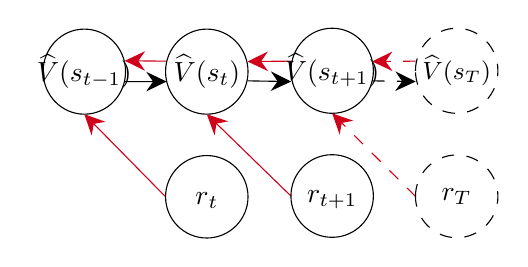
\begin{tikzpicture}[x=0.75pt,y=0.75pt,yscale=-1,xscale=1]
        
        %Straight Lines [id:da2592063600931961] 
        \draw [color={rgb, 255:red, 208; green, 2; blue, 27 }  ,draw opacity=1 ]   (282.5,135.16) -- (300.67,135.02) ;
        \draw [shift={(279.5,135.18)}, rotate = 359.55] [fill={rgb, 255:red, 208; green, 2; blue, 27 }  ,fill opacity=1 ][line width=0.08]  [draw opacity=0] (9.82,-4.72) -- (0,0) -- (9.82,4.72) -- (6.52,0) -- cycle    ;
        %Straight Lines [id:da41585806917853485] 
        \draw [color={rgb, 255:red, 208; green, 2; blue, 27 }  ,draw opacity=1 ]   (223.33,134.87) -- (240.67,135.02) ;
        \draw [shift={(220.33,134.85)}, rotate = 0.47] [fill={rgb, 255:red, 208; green, 2; blue, 27 }  ,fill opacity=1 ][line width=0.08]  [draw opacity=0] (9.82,-4.72) -- (0,0) -- (9.82,4.72) -- (6.52,0) -- cycle    ;
        %Shape: Ellipse [id:dp31493856088290983] 
        \draw   (181,140.07) .. controls (181,128.75) and (189.89,119.58) .. (200.86,119.58) .. controls (211.83,119.58) and (220.72,128.75) .. (220.72,140.07) .. controls (220.72,151.4) and (211.83,160.57) .. (200.86,160.57) .. controls (189.89,160.57) and (181,151.4) .. (181,140.07) -- cycle ;
        %Shape: Ellipse [id:dp5103941395609547] 
        \draw  [dash pattern={on 4.5pt off 4.5pt}] (360.4,139.66) .. controls (360.4,128.34) and (369.29,119.16) .. (380.26,119.16) .. controls (391.23,119.16) and (400.12,128.34) .. (400.12,139.66) .. controls (400.12,150.98) and (391.23,160.16) .. (380.26,160.16) .. controls (369.29,160.16) and (360.4,150.98) .. (360.4,139.66) -- cycle ;
        %Straight Lines [id:da30559831832260953] 
        \draw [color={rgb, 255:red, 0; green, 0; blue, 0 }  ,draw opacity=1 ]   (220.07,144.9) -- (237.5,144.86) ;
        \draw [shift={(240.5,144.85)}, rotate = 539.86] [fill={rgb, 255:red, 0; green, 0; blue, 0 }  ,fill opacity=1 ][line width=0.08]  [draw opacity=0] (9.82,-4.72) -- (0,0) -- (9.82,4.72) -- (6.52,0) -- cycle    ;
        %Shape: Ellipse [id:dp12377292733336898] 
        \draw  [color={rgb, 255:red, 0; green, 0; blue, 0 }  ,draw opacity=1 ] (240,140.07) .. controls (240,128.75) and (248.89,119.58) .. (259.86,119.58) .. controls (270.83,119.58) and (279.72,128.75) .. (279.72,140.07) .. controls (279.72,151.4) and (270.83,160.57) .. (259.86,160.57) .. controls (248.89,160.57) and (240,151.4) .. (240,140.07) -- cycle ;
        %Shape: Ellipse [id:dp9248757796917767] 
        \draw   (300.4,139.66) .. controls (300.4,128.34) and (309.29,119.16) .. (320.26,119.16) .. controls (331.23,119.16) and (340.12,128.34) .. (340.12,139.66) .. controls (340.12,150.98) and (331.23,160.16) .. (320.26,160.16) .. controls (309.29,160.16) and (300.4,150.98) .. (300.4,139.66) -- cycle ;
        %Straight Lines [id:da050274800713848156] 
        \draw [color={rgb, 255:red, 208; green, 2; blue, 27 }  ,draw opacity=1 ]   (202.96,162.71) -- (240,200.37) ;
        \draw [shift={(200.86,160.57)}, rotate = 45.48] [fill={rgb, 255:red, 208; green, 2; blue, 27 }  ,fill opacity=1 ][line width=0.08]  [draw opacity=0] (9.82,-4.72) -- (0,0) -- (9.82,4.72) -- (6.52,0) -- cycle    ;
        %Straight Lines [id:da7059353635730191] 
        \draw [color={rgb, 255:red, 208; green, 2; blue, 27 }  ,draw opacity=1 ]   (262.01,162.66) -- (300.4,200) ;
        \draw [shift={(259.86,160.57)}, rotate = 44.2] [fill={rgb, 255:red, 208; green, 2; blue, 27 }  ,fill opacity=1 ][line width=0.08]  [draw opacity=0] (9.82,-4.72) -- (0,0) -- (9.82,4.72) -- (6.52,0) -- cycle    ;
        %Straight Lines [id:da17885982011746426] 
        \draw [color={rgb, 255:red, 208; green, 2; blue, 27 }  ,draw opacity=1 ] [dash pattern={on 4.5pt off 4.5pt}]  (322.38,162.28) -- (360.4,200.16) ;
        \draw [shift={(320.26,160.16)}, rotate = 44.9] [fill={rgb, 255:red, 208; green, 2; blue, 27 }  ,fill opacity=1 ][line width=0.08]  [draw opacity=0] (9.82,-4.72) -- (0,0) -- (9.82,4.72) -- (6.52,0) -- cycle    ;
        %Shape: Ellipse [id:dp3523005799699832] 
        \draw  [dash pattern={on 4.5pt off 4.5pt}] (360.4,200.16) .. controls (360.4,189.16) and (369.29,180.23) .. (380.26,180.23) .. controls (391.23,180.23) and (400.12,189.16) .. (400.12,200.16) .. controls (400.12,211.17) and (391.23,220.09) .. (380.26,220.09) .. controls (369.29,220.09) and (360.4,211.17) .. (360.4,200.16) -- cycle ;
        %Shape: Ellipse [id:dp3509500153089894] 
        \draw   (300.4,200) .. controls (300.4,189) and (309.29,180.09) .. (320.26,180.09) .. controls (331.23,180.09) and (340.12,189) .. (340.12,200) .. controls (340.12,210.99) and (331.23,219.9) .. (320.26,219.9) .. controls (309.29,219.9) and (300.4,210.99) .. (300.4,200) -- cycle ;
        %Shape: Ellipse [id:dp17336392317383575] 
        \draw  [color={rgb, 255:red, 0; green, 0; blue, 0 }  ,draw opacity=1 ] (240,200.37) .. controls (240,189.4) and (248.89,180.5) .. (259.86,180.5) .. controls (270.83,180.5) and (279.72,189.4) .. (279.72,200.37) .. controls (279.72,211.34) and (270.83,220.23) .. (259.86,220.23) .. controls (248.89,220.23) and (240,211.34) .. (240,200.37) -- cycle ;
        %Straight Lines [id:da21459790152477998] 
        \draw [color={rgb, 255:red, 0; green, 0; blue, 0 }  ,draw opacity=1 ]   (279.5,144.52) -- (297.5,144.8) ;
        \draw [shift={(300.5,144.85)}, rotate = 180.91] [fill={rgb, 255:red, 0; green, 0; blue, 0 }  ,fill opacity=1 ][line width=0.08]  [draw opacity=0] (9.82,-4.72) -- (0,0) -- (9.82,4.72) -- (6.52,0) -- cycle    ;
        %Straight Lines [id:da8588950475203374] 
        \draw [color={rgb, 255:red, 208; green, 2; blue, 27 }  ,draw opacity=1 ] [dash pattern={on 4.5pt off 4.5pt}]  (342.5,135.16) -- (360.67,135.02) ;
        \draw [shift={(339.5,135.18)}, rotate = 359.55] [fill={rgb, 255:red, 208; green, 2; blue, 27 }  ,fill opacity=1 ][line width=0.08]  [draw opacity=0] (9.82,-4.72) -- (0,0) -- (9.82,4.72) -- (6.52,0) -- cycle    ;
        %Straight Lines [id:da9169375689094925] 
        \draw [color={rgb, 255:red, 0; green, 0; blue, 0 }  ,draw opacity=1 ] [dash pattern={on 4.5pt off 4.5pt}]  (339.5,144.52) -- (357.5,144.8) ;
        \draw [shift={(360.5,144.85)}, rotate = 180.91] [fill={rgb, 255:red, 0; green, 0; blue, 0 }  ,fill opacity=1 ][line width=0.08]  [draw opacity=0] (9.82,-4.72) -- (0,0) -- (9.82,4.72) -- (6.52,0) -- cycle    ;
        
        % Text Node
        \draw (320.26,201.59) node    {$r_{t+1}$};
        % Text Node
        \draw (200.86,140.07) node    {$\widehat{V}(s_{t-1})$};
        % Text Node
        \draw (320.26,139.66) node    {$\widehat{V}(s_{t+1})$};
        % Text Node
        \draw (380.26,139.66) node  [font=\small]  {$\widehat{V}(s_{T})$};
        % Text Node
        \draw (259.86,202) node  [color={rgb, 255:red, 208; green, 9; blue, 2 }  ,opacity=1 ]  {$\textcolor[rgb]{0,0,0}{r}\textcolor[rgb]{0,0,0}{_{t}}$};
        % Text Node
        \draw (259.86,140.07) node  [color={rgb, 255:red, 208; green, 9; blue, 2 }  ,opacity=1 ]  {$\textcolor[rgb]{0,0,0}{\widehat{V}}\textcolor[rgb]{0,0,0}{(s_{t})}$};
        % Text Node
        \draw (380.26,200.16) node    {$r_{T}$};

        \end{tikzpicture}
    \end{adjustbox}
  \end{center}
\caption[\textbf{Graphical representation of TD Learning}]{Red arrows indicate the flow of the computations for deriving $\delta$ and updating $\widehat{V}$ expressed by equations \ref{td_error} and \ref{td_update}. Black arrows instead indicate the changes of $\widehat{V}$ moving from $s$ to $s_{t+1}$. Solid circles indicate states which have already been observed while dashed ones represent future not-yet observed states.}
\label{fig: td_learning}
\end{figure}
McClure \textit{et. al.} proposed that incentive salience is represented by $V$ as defined in equation \ref{td_v} while the error signal expressed by equation \ref{td_error} represents the activity of dopaminergic neurons with the dual function of driving the attribution of incentive salience (through reward prediction error coding as specified in section \ref{incentive_salience}) and guiding the previously mentioned action selection process \cite{schultz1997neural,mcclure2003computational,o2003temporal}. However, in later work, Zhang \textit{et. al.} highlighted the fact that the model proposed by McClure \textit{et. al.} fails to take into account an important part of the original incentive salience hypothesis: the dynamic modulation produced by the individual's internal state (see section \ref{wanting}) \cite{toates1994comparing,mcclure2003computational,berridge2004motivation,zhang2009neural,tindell2009dynamic,berridge2012prediction}. Zhang \textit{et. al.} therefore proposed a modification of the original TD Learning model to include a modulatory factor $k \in [0, +\infty]$ which can enhance ($k > 1$), dampen or even revert ($k < 1$) previously learned incentive salience values
\begin{align}
    \label{zhang_td_v}
    V(s_t) = E[\tilde{r}(r_{t+1},k_{t}) + \gamma V(s_{t+1})]
\end{align}
here $\tilde{r}(.,.)$ is a function of two variables and can assume either an additive or multiplicative form \footnote{See \cite{zhang2009neural} for detailed description of the two forms and their functional differences.}. The main difference between the approaches of McClure \textit{et. al.} and Zhang \textit{et. al.} lies in the interpretation of $V$. Both authors see it as a combination of cached value (i.e. what has been learned from past experiences) and expectation over future $r$ but for McClure \textit{et. al.} all the future $r$ have the same weight while for Zhang \textit{et. al.} the state of the individual dynamically modulates the weighting of $r$. Using the notation from section \ref{incentive_salience}, we can say that the interaction $s$ between $I$ and $O$ at time $t_{+1}$ arises from the $V$ (i.e. incentive salience) generated after $s_{t}$. The mismatch between the predicted amount of reward and the actual reward received at time $t_{+1}$ generates an error signal that allows $I$ to learn about the "correct" magnitude of $V(s_{t})$ \cite{schultz2017reward} . As an example, an individual may anticipate that eating their favourite meal would be a rewarding experience but instead (for some reason) it was underwhelming. They therefore reduce the salience previously attributed to it. Importantly, $V(s_{t})$ does not just encompass the previous history of interactions between an individual and an object but also the current state of the individual themselves: the individual has learned from long experience that eating is a pleasurable activity but currently, since they are sated they do not expect much reward from doing it again in the near future.  \\
\\
In this view, motivation can be described as a mechanism that guides the interaction between individuals and objects. It controls and selects behaviours which are expected to lead to pleasurable outcomes for the individual (i.e. incentives or reward). These expectancies are the product of a learning process that can be modulated by the internal state of the individual. Therefore, from a behavioural point of view, an objects $O$ can acquire salience for an individual $I$ conditioned on its capacity to elicit rewarding experience $r$ \cite{berridge1998role,mcclure2003computational}. The amount of attributed salience is a valued representation of $O$ generated by $I$ and controls how likely and intense future interactions between the two will be. \cite{berridge1998role,mcclure2003computational}. Let $B$ represents the strength of an interaction between $I$ and $O$, $r$ a measure of how rewarding the interaction with $O$ is perceived to be and $V$ the generated attributed incentive salience.
\begin{figure}[h]
  \begin{center}
    \begin{adjustbox}{width=0.5\columnwidth}

        \tikzset{every picture/.style={line width=0.75pt}}
        
        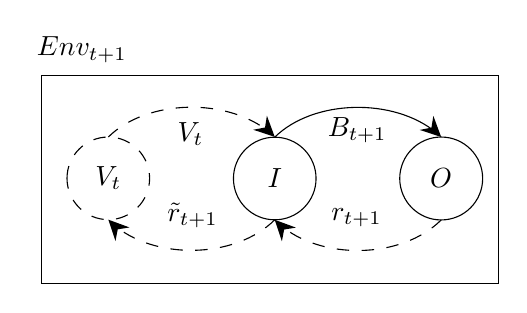
\begin{tikzpicture}[x=0.75pt,y=0.75pt,yscale=-1,xscale=1]
        
        %Shape: Circle [id:dp8739177923629333] 
        \draw   (123.48,130.05) .. controls (123.48,119.06) and (132.39,110.15) .. (143.38,110.15) .. controls (154.37,110.15) and (163.28,119.06) .. (163.28,130.05) .. controls (163.28,141.04) and (154.37,149.95) .. (143.38,149.95) .. controls (132.39,149.95) and (123.48,141.04) .. (123.48,130.05) -- cycle ;
        %Curve Lines [id:da2726669379173874] 
        \draw    (143.38,110.15) .. controls (161.99,91.83) and (200.82,90.88) .. (221.41,108.12) ;
        \draw [shift={(223.57,110.07)}, rotate = 224.02] [fill={rgb, 255:red, 0; green, 0; blue, 0 }  ][line width=0.08]  [draw opacity=0] (9.82,-4.72) -- (0,0) -- (9.82,4.72) -- (6.52,0) -- cycle    ;
        %Curve Lines [id:da4485667818478689] 
        \draw  [dash pattern={on 4.5pt off 4.5pt}]  (223.57,150.02) .. controls (204.36,169.14) and (165.2,169.5) .. (145.45,151.93) ;
        \draw [shift={(143.38,149.95)}, rotate = 405.89] [fill={rgb, 255:red, 0; green, 0; blue, 0 }  ][line width=0.08]  [draw opacity=0] (9.82,-4.72) -- (0,0) -- (9.82,4.72) -- (6.52,0) -- cycle    ;
        %Shape: Circle [id:dp8060688469385651] 
        \draw   (203.6,130.05) .. controls (203.6,119.01) and (212.54,110.07) .. (223.57,110.07) .. controls (234.6,110.07) and (243.55,119.01) .. (243.55,130.05) .. controls (243.55,141.08) and (234.6,150.02) .. (223.57,150.02) .. controls (212.54,150.02) and (203.6,141.08) .. (203.6,130.05) -- cycle ;
        %Shape: Rectangle [id:dp6054697635081123] 
        \draw   (31.2,80.5) -- (251.2,80.5) -- (251.2,180.83) -- (31.2,180.83) -- cycle ;
        %Shape: Circle [id:dp6091430023771998] 
        \draw  [dash pattern={on 4.5pt off 4.5pt}] (43.29,129.97) .. controls (43.29,118.98) and (52.2,110.07) .. (63.19,110.07) .. controls (74.18,110.07) and (83.09,118.98) .. (83.09,129.97) .. controls (83.09,140.96) and (74.18,149.87) .. (63.19,149.87) .. controls (52.2,149.87) and (43.29,140.96) .. (43.29,129.97) -- cycle ;
        %Curve Lines [id:da9876749075069771] 
        \draw  [dash pattern={on 4.5pt off 4.5pt}]  (143.38,149.95) .. controls (124.17,169.06) and (85.01,169.42) .. (65.26,151.85) ;
        \draw [shift={(63.19,149.87)}, rotate = 405.89] [fill={rgb, 255:red, 0; green, 0; blue, 0 }  ][line width=0.08]  [draw opacity=0] (9.82,-4.72) -- (0,0) -- (9.82,4.72) -- (6.52,0) -- cycle    ;
        %Curve Lines [id:da9412329086480583] 
        \draw  [dash pattern={on 4.5pt off 4.5pt}]  (63.19,110.07) .. controls (81.8,91.76) and (120.63,90.8) .. (141.21,108.05) ;
        \draw [shift={(143.38,110)}, rotate = 224.02] [fill={rgb, 255:red, 0; green, 0; blue, 0 }  ][line width=0.08]  [draw opacity=0] (9.82,-4.72) -- (0,0) -- (9.82,4.72) -- (6.52,0) -- cycle    ;
        
        % Text Node
        \draw (143.38,130.05) node  [font=\normalsize]  {$I$};
        % Text Node
        \draw (223.57,130.05) node  [font=\normalsize]  {$O$};
        % Text Node
        \draw (183.14,106.95) node  [font=\normalsize]  {$B_{t+1}$};
        % Text Node
        \draw (182.81,148.81) node  [font=\normalsize]  {$r_{t+1}$};
        % Text Node
        \draw (50.45,68.01) node  [font=\normalsize,rotate=-0.16]  {$Env_{t+1}$};
        % Text Node
        \draw (63.19,129.97) node  [font=\normalsize]  {$V_{t}$};
        % Text Node
        \draw (103.81,147.81) node  [font=\normalsize]  {$\tilde{r}_{t+1}$};
        % Text Node
        \draw (102.81,108.81) node  [font=\normalsize]  {$V_{t}$};
        \end{tikzpicture}
    \end{adjustbox}
  \end{center}
\caption[\textbf{The process of incentive salience attribution}]{Solid and dashed elements represent respectively observable (i.e. behavioural) and latent aspects of the process. The individual and the object that they interact with are indicated by $I$ and $O$. The strength of the interaction is represented by $B$. The salience that $I$ attributes to $O$ is expressed by $V$ while $r$ and $\tilde{r}$ are the experienced reward and its weighted version produced by the state of $I$. All the contextual factors influencing both the amount of $r$ perceived and the magnitude of $B$ produced are represented by $Env$. The dynamical natures of the process is expressed though the arbitrary temporal unit $t$.}
\label{fig: incs}
\end{figure}
Following Figure \ref{fig: incs}, at time $t+1$ an individual will produce an interaction with an object of strength $B$ according to the previous $V_{t}$. If we recall from section \ref{learning}, this process relies heavily on learning mechanisms making $V$ by nature dynamic and mutable. It should be noted that $B$ can be represented as a multidimensional variable defined by the instrumental behaviours conventionally used for assessing the \emph{wanting} component in animal studies (e.g. frequency, amount and duration of feeding behaviours like bites, nibbles and sniffs) \cite{berridge1998role}. During and after the interaction $I$ will experience a variable degree of reward $r_{t+1}$ that, weighted by their internal state, will then be used for updating $V_{t}$.  It is worth noting that the individual's internal state is not the only factor involved in the modulation of $r$, also the context in which $I$ and $O$ interact ($Env_{t+1}$ in Figure \ref{fig: incs}) seems to contribute to this \cite{palminteri2015contextual}. Following the idea presented in section \ref{manifold_rep_incentive_salience}, the latent state defined by $V$ could be represented as a manifold defined by the activity of those regions responsible for the attribution of incentive salience. Moreover, given the strong coupling between attributed incentive salience and behaviour \cite{berridge1998role} we would also expect the structure of this manifold to be a suitable descriptor of the behavioural aspects of attributed incentive salience.

\paragraph*{\textbf{From TD to Supervised Learning}}
\label{td_to_supervised}The approaches discussed above frame the estimation of attributed incentive salience as a reinforcement learning task. This requires the simulation of a sequence of interactions between $I$ and $O$ and the concomitant delivery of $r$  \cite{schultz1997neural,mcclure2003computational,zhang2009neural}. However, it is not always straightforward to replicate these interactions in real world scenarios, especially when dealing with human participants. The control on the internal state of $I$ and amount of $r$ delivered that McClure and Zhang assume is usually based on strict assumptions and can be achieved only in controlled experimental settings \cite{mcclure2003computational,zhang2009neural}. As an alternative solution for inferring $V$ outside the laboratory we propose to learn its manifold structure through supervised learning. Differently to what reported in the literature \cite{calhoun2019unsupervised, mccullough2021unsupervised, luxem2020identifying, pereira2020quantifying, shi2021learning} we argue that in this case the use of supervised in place of un-supervised techniques is to be preferred. Indeed, since we are dealing exclusively with behavioural data and trying to solve an inverse problem  we would like to learn a manifold structure which is not just a generic indicator of behavioural phenotype \cite{luxem2020identifying} but also obeys to specific functional constrains.\\
\\
In this approach, an experimenter gathers data on a set of interactions between $I$ and $O$ and let a learning algorithm to estimate two functions:
\begin{gather}
\label{supervised_v}
    V(s_{t}) = f^{1}(O, \tilde{r_{t}}, V(s_{t-1}); \theta^{1}) \\
    r_{t+1} = f^{2}(V(s_{t}); \theta^{2}) \nonumber
\end{gather}
here $f^{1}$ and $f^{2}$ are arbitrarily complex functions while $\theta^{1}$ and $\theta^{2}$ are parameters that the learning algorithm has to infer. The future reward that an individual expects after an interaction with an object is produced by the current level of attributed salience, which  itself is a function of the current internal state of the individual (expressed through the amount of reward just experienced) and the incentive salience previously attributed to the object. It is important to note that the two functions above need to be recursive over all $s \in S$ (see equations \ref{td_v} and \ref{zhang_td_v}) in order to provide $V(s_{t})$ with the dual purpose of caching all the past $V$ and being a suitable predictor for all the $r$. This formulation however still requires a measure of the $r$ experienced by $I$ (or more precisely its weighted version $\tilde{r}$) after interacting with $O$, which is not easily accessible. However, Thorndike's law of effect \cite{thorndike1927law} and Skinner's operant conditioning principles \cite{skinner1965science} suggest that $r$, which  like $V$ is a non observable latent variable, manifests itself through the intensity of interactions between $I$ and $O$ (i.e. $B$ in Figure \ref{fig: incs}): the frequency and amount of object-directed behaviours increase or decrease as a function of the rewards an individual expects to receive \cite{berridge2004motivation,schultz2017reward}. Since $V(s_{t})$ predicts how much $r$ an $I$ expects to receive from interacting with $O$, we should also expect the strength of their future interactions to be a function of $V(s_{t})$. This can be represented re-arranging the equations in \ref{supervised_v} in a more compact form as a chain of functions
\begin{align}
\label{supervised_b}
    B_{t+1} = f^{2}(f^{1}(O, B_{t}, V(s_{t-1}); \theta^{1});  \theta^{2})
\end{align}
To approximate the above expression, a learning algorithm would require records of behaviours generated by individuals while interacting with a diverse set of potentially rewarding objects. Here, we argue that video games are one way to obtain this type of data at scale while also achieving some level of ecological validity.

\subsection{Video Games and Telemetry}
\label{videogame_telemetries}
As we highlighted in chapter \ref{chapter_lit_review}, interacting with video games is a volitional activity driven largely by the capacity of the games to provide pleasurable experiences \cite{boyle2012engagement}. Behaviour within the game is best understood as the result of a value attribution process similar to that of secondary reward objects (see section \ref{incentive_salience}). Indeed, it appears that the play behaviour is often produced and maintained by the structural characteristics of the game (e.g. game mechanics) \cite{king2010video} which, working like conventional reinforcement mechanisms \cite{chumbley2006affect,wang2011game,phillips2013videogame,avserivskis2017computational}, produce effects similar to operant conditioning \cite{skinner1965science}. Although caution should be applied when complex activities are investigated using neuroimaging techniques, evidence suggest that the maintenance of video games playing behaviour engages the same cortico-striatal structures \cite{hoeft2008gender,mathiak2011reward,cole2012interactivity,klasen2012neural,lorenz2015video,gleich2017functional} and neurotransmitters \cite{koepp1998evidence} involved in reward processing. This, seems also supported at the behavioural level where the ammount of experienced in-game reward appears to play a role in controlling how likely is an individual to keep engaging in playing behaviour \cite{agarwal2017quitting, steyvers2019joint}. This, in conjunction with a growing literature highlighting similarities between certain video game mechanics and activities driven by secondary rewards (e.g. gambling) \cite{king2010role,drummond2018video,zendle2018video}, corroborates the idea that video games are able to elicit behavioural responses through incentive mechanics. In this view, video games with different structural characteristics could be seen as objects possessing rewarding properties that heavily depend on the individuals interacting with them (e.g. an individual's preference for a specific game mechanic). Hence, similarly to the process specified in chapter \ref{chapter_lit_review}, we can expect that through repeated interactions, an individual will experience varying degrees of reward determined by their internal state and the characteristics of the game. These interactions will produce continuous adjustments in the level of saliency attributed to playing that specific game which in turn will influence the frequency and amount of future interactions with that same game. Other than offering a context for observing the process of incentive salience attribution, video games allow us to obtain large volumes of behavioural data (similar to those mentioned in chapter \ref{chapter_lit_review}) in a naturalistic fashion. This is made possible by the widespread practice of obtaining high frequency records (i.e. telemetry\footnote{See \cite{el2016game} for a more technical description of telemetry in video games.}) of players' behaviour during the game \cite{drachen2015behavioral}. This approach, despite offering less control and rigour than conventional experimental procedures, allows us to obtain a more faithful representation of natural behaviour (similarly to field studies) while avoiding some of the limitations connected with laboratory-based studies (e.g. sampling and observer biases).
\newline
\newline
In order to use this type of behavioural data to model attributed incentive salience, a learning algorithm should possess the following properties. First, it should be scalable and noise resilient, to leverage large volumes of naturalistic data in an efficient and effective manner. Second, it should be able to approximate arbitrarily complex functions, given that the shape of the functions specified in equation \ref{td_to_supervised} is not known a-priori. And finally, it should be able to produce an approximation of $V(s_{t})$ that can be inspected in order to evaluate if its functional properties can be compared with those of attributed incentive salience. Artificial Neural Networks (ANNs) appear to satisfy these requirements.

\subsection{Artificial Neural Networks}
\label{artificial_neural_networks}
In their conventional form, ANNs can be seen as chains of nested functions (the layers of the network). These layers are vector valued (there are multiple units or neurons in each layer) and organized as directed acyclic computational graphs (information only flows forward). When the number of layers is greater than two, the prefix "deep" is usually applied \cite{bengio2017deep}. The goal of this ensemble of functions is to create a mapping between an input $x$ and a target $y$. Following the example illustrated in Figure \ref{fig: ffnn}, given the set of parameters $\Theta = \{\theta^1, \theta^2 \}$ an ANN would first infer a function $h = f(x;\theta^{1})$, mapping the input to a new representation $h$. The same representation $h$ would then become the input of a second function $\widehat{y} = f^{1}(h;\theta^{2})$ which produces an estimate of the target \cite{bengio2017deep}. In this sense, we can think of each layer as a collection of many non-linear vector to scalar functions taking the previous layer as input and generating the units for the layer that follows \cite{bengio2017deep}. By increasing the number of layers and units, ANNs can approximate an extremely large class of functions \cite{rumelhart1986learning}.
\begin{figure}
    \begin{center}
        \begin{adjustbox}{width=0.4\textwidth}
            \tikzset{every picture/.style={line width=0.75pt}} %set default line width to 0.75pt        
            
            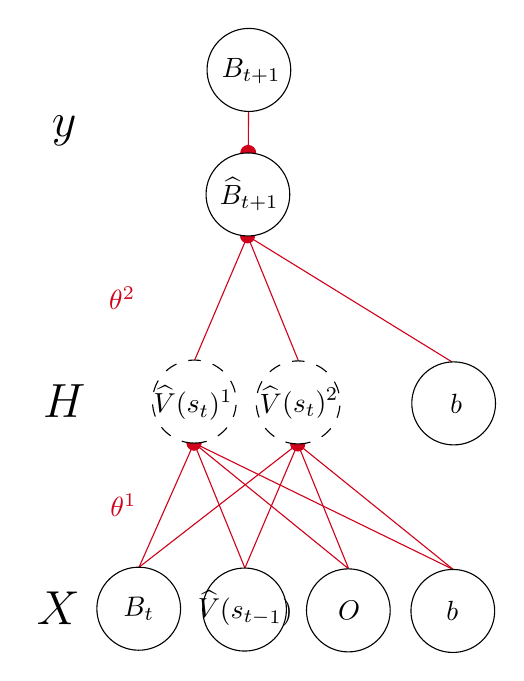
\begin{tikzpicture}[x=0.75pt,y=0.75pt,yscale=-1,xscale=1]
            %uncomment if require: \path (0,350); %set diagram left start at 0, and has height of 350
            
            %Straight Lines [id:da8866607252953388] 
            \draw [color={rgb, 255:red, 208; green, 2; blue, 27 }  ,draw opacity=1 ]   (227.88,279.44) -- (254.36,219.65) ;
            \draw [shift={(254.36,219.65)}, rotate = 293.89] [color={rgb, 255:red, 208; green, 2; blue, 27 }  ,draw opacity=1 ][fill={rgb, 255:red, 208; green, 2; blue, 27 }  ,fill opacity=1 ][line width=0.75]      (0, 0) circle [x radius= 3.02, y radius= 3.02]   ;
            %Straight Lines [id:da0731191645042184] 
            \draw [color={rgb, 255:red, 208; green, 2; blue, 27 }  ,draw opacity=1 ]   (254.68,179.65) -- (280.16,119.85) ;
            \draw [shift={(280.16,119.85)}, rotate = 293.08] [color={rgb, 255:red, 208; green, 2; blue, 27 }  ,draw opacity=1 ][fill={rgb, 255:red, 208; green, 2; blue, 27 }  ,fill opacity=1 ][line width=0.75]      (0, 0) circle [x radius= 3.02, y radius= 3.02]   ;
            %Straight Lines [id:da4826752085294559] 
            \draw [color={rgb, 255:red, 208; green, 2; blue, 27 }  ,draw opacity=1 ]   (304.68,180.05) -- (280.16,119.85) ;
            \draw [shift={(280.16,119.85)}, rotate = 247.84] [color={rgb, 255:red, 208; green, 2; blue, 27 }  ,draw opacity=1 ][fill={rgb, 255:red, 208; green, 2; blue, 27 }  ,fill opacity=1 ][line width=0.75]      (0, 0) circle [x radius= 2.01, y radius= 2.01]   ;
            %Straight Lines [id:da39539248901414714] 
            \draw [color={rgb, 255:red, 208; green, 2; blue, 27 }  ,draw opacity=1 ]   (328.88,280.25) -- (304.36,220.05) ;
            \draw [shift={(304.36,220.05)}, rotate = 247.84] [color={rgb, 255:red, 208; green, 2; blue, 27 }  ,draw opacity=1 ][fill={rgb, 255:red, 208; green, 2; blue, 27 }  ,fill opacity=1 ][line width=0.75]      (0, 0) circle [x radius= 3.02, y radius= 3.02]   ;
            %Straight Lines [id:da8990891706173756] 
            \draw [color={rgb, 255:red, 208; green, 2; blue, 27 }  ,draw opacity=1 ]   (278.88,279.85) -- (254.36,219.65) ;
            \draw [shift={(254.36,219.65)}, rotate = 247.84] [color={rgb, 255:red, 208; green, 2; blue, 27 }  ,draw opacity=1 ][fill={rgb, 255:red, 208; green, 2; blue, 27 }  ,fill opacity=1 ][line width=0.75]      (0, 0) circle [x radius= 3.02, y radius= 3.02]   ;
            %Straight Lines [id:da1147021220204143] 
            \draw [color={rgb, 255:red, 208; green, 2; blue, 27 }  ,draw opacity=1 ]   (328.88,280.25) -- (254.36,219.65) ;
            \draw [shift={(254.36,219.65)}, rotate = 219.12] [color={rgb, 255:red, 208; green, 2; blue, 27 }  ,draw opacity=1 ][fill={rgb, 255:red, 208; green, 2; blue, 27 }  ,fill opacity=1 ][line width=0.75]      (0, 0) circle [x radius= 3.02, y radius= 3.02]   ;
            %Straight Lines [id:da30405558125224674] 
            \draw [color={rgb, 255:red, 208; green, 2; blue, 27 }  ,draw opacity=1 ]   (278.88,279.85) -- (304.36,220.05) ;
            \draw [shift={(304.36,220.05)}, rotate = 293.08] [color={rgb, 255:red, 208; green, 2; blue, 27 }  ,draw opacity=1 ][fill={rgb, 255:red, 208; green, 2; blue, 27 }  ,fill opacity=1 ][line width=0.75]      (0, 0) circle [x radius= 3.02, y radius= 3.02]   ;
            %Straight Lines [id:da7841365763851936] 
            \draw [color={rgb, 255:red, 208; green, 2; blue, 27 }  ,draw opacity=1 ]   (227.88,279.44) -- (304.36,220.05) ;
            \draw [shift={(304.36,220.05)}, rotate = 322.17] [color={rgb, 255:red, 208; green, 2; blue, 27 }  ,draw opacity=1 ][fill={rgb, 255:red, 208; green, 2; blue, 27 }  ,fill opacity=1 ][line width=0.75]      (0, 0) circle [x radius= 3.02, y radius= 3.02]   ;
            %Straight Lines [id:da5618158283475858] 
            \draw [color={rgb, 255:red, 208; green, 2; blue, 27 }  ,draw opacity=1 ]   (379.21,280.52) -- (304.36,220.05) ;
            \draw [shift={(304.36,220.05)}, rotate = 218.93] [color={rgb, 255:red, 208; green, 2; blue, 27 }  ,draw opacity=1 ][fill={rgb, 255:red, 208; green, 2; blue, 27 }  ,fill opacity=1 ][line width=0.75]      (0, 0) circle [x radius= 3.02, y radius= 3.02]   ;
            %Straight Lines [id:da4509011415852858] 
            \draw [color={rgb, 255:red, 208; green, 2; blue, 27 }  ,draw opacity=1 ]   (378.61,180.51) -- (280.16,119.85) ;
            \draw [shift={(280.16,119.85)}, rotate = 211.64] [color={rgb, 255:red, 208; green, 2; blue, 27 }  ,draw opacity=1 ][fill={rgb, 255:red, 208; green, 2; blue, 27 }  ,fill opacity=1 ][line width=0.75]      (0, 0) circle [x radius= 3.02, y radius= 3.02]   ;
            %Straight Lines [id:da7242656967921071] 
            \draw [color={rgb, 255:red, 208; green, 2; blue, 27 }  ,draw opacity=1 ]   (379.21,280.52) -- (254.36,219.65) ;
            \draw [shift={(254.36,219.65)}, rotate = 205.99] [color={rgb, 255:red, 208; green, 2; blue, 27 }  ,draw opacity=1 ][fill={rgb, 255:red, 208; green, 2; blue, 27 }  ,fill opacity=1 ][line width=0.75]      (0, 0) circle [x radius= 3.02, y radius= 3.02]   ;
            %Shape: Ellipse [id:dp9097533963365589] 
            \draw  [fill={rgb, 255:red, 255; green, 255; blue, 255 }  ,fill opacity=1 ][dash pattern={on 4.5pt off 4.5pt}] (304.36,220.05) .. controls (293.22,219.96) and (284.26,210.94) .. (284.35,199.89) .. controls (284.44,188.84) and (293.54,179.96) .. (304.68,180.05) .. controls (315.82,180.14) and (324.77,189.17) .. (324.69,200.21) .. controls (324.6,211.26) and (315.5,220.14) .. (304.36,220.05) -- cycle ;
            %Shape: Ellipse [id:dp9467435778420286] 
            \draw  [fill={rgb, 255:red, 255; green, 255; blue, 255 }  ,fill opacity=1 ][dash pattern={on 4.5pt off 4.5pt}] (254.36,219.65) .. controls (243.22,219.56) and (234.27,210.53) .. (234.36,199.49) .. controls (234.44,188.44) and (243.54,179.56) .. (254.68,179.65) .. controls (265.82,179.74) and (274.78,188.77) .. (274.69,199.81) .. controls (274.6,210.86) and (265.5,219.74) .. (254.36,219.65) -- cycle ;
            %Shape: Ellipse [id:dp4514100854948462] 
            \draw  [fill={rgb, 255:red, 255; green, 255; blue, 255 }  ,fill opacity=1 ] (379.29,220.52) .. controls (368.15,220.43) and (359.2,211.4) .. (359.29,200.36) .. controls (359.37,189.31) and (368.47,180.43) .. (379.61,180.52) .. controls (390.75,180.61) and (399.71,189.64) .. (399.62,200.68) .. controls (399.53,211.73) and (390.43,220.61) .. (379.29,220.52) -- cycle ;
            %Shape: Ellipse [id:dp2836578028815524] 
            \draw  [fill={rgb, 255:red, 255; green, 255; blue, 255 }  ,fill opacity=1 ] (227.56,319.44) .. controls (216.42,319.35) and (207.46,310.32) .. (207.55,299.28) .. controls (207.64,288.23) and (216.74,279.35) .. (227.88,279.44) .. controls (239.02,279.53) and (247.97,288.56) .. (247.89,299.6) .. controls (247.8,310.65) and (238.7,319.53) .. (227.56,319.44) -- cycle ;
            %Shape: Ellipse [id:dp10987171532240936] 
            \draw  [fill={rgb, 255:red, 255; green, 255; blue, 255 }  ,fill opacity=1 ] (278.56,319.85) .. controls (267.42,319.76) and (258.46,310.73) .. (258.55,299.69) .. controls (258.64,288.64) and (267.74,279.76) .. (278.88,279.85) .. controls (290.02,279.94) and (298.97,288.96) .. (298.88,300.01) .. controls (298.79,311.06) and (289.69,319.94) .. (278.56,319.85) -- cycle ;
            %Shape: Ellipse [id:dp5734471221931936] 
            \draw  [fill={rgb, 255:red, 255; green, 255; blue, 255 }  ,fill opacity=1 ] (328.56,320.25) .. controls (317.42,320.16) and (308.46,311.13) .. (308.55,300.09) .. controls (308.64,289.04) and (317.74,280.16) .. (328.88,280.25) .. controls (340.01,280.34) and (348.97,289.37) .. (348.88,300.41) .. controls (348.79,311.46) and (339.69,320.34) .. (328.56,320.25) -- cycle ;
            %Shape: Ellipse [id:dp8405299754625457] 
            \draw  [fill={rgb, 255:red, 255; green, 255; blue, 255 }  ,fill opacity=1 ] (378.89,320.52) .. controls (367.75,320.43) and (358.79,311.4) .. (358.88,300.36) .. controls (358.97,289.31) and (368.07,280.43) .. (379.21,280.52) .. controls (390.35,280.61) and (399.3,289.64) .. (399.21,300.68) .. controls (399.13,311.73) and (390.03,320.61) .. (378.89,320.52) -- cycle ;
            %Straight Lines [id:da531681756338569] 
            \draw [color={rgb, 255:red, 208; green, 2; blue, 27 }  ,draw opacity=1 ]   (280.48,79.86) -- (280.64,59.86) ;
            \draw [shift={(280.48,79.86)}, rotate = 270.46] [color={rgb, 255:red, 208; green, 2; blue, 27 }  ,draw opacity=1 ][fill={rgb, 255:red, 208; green, 2; blue, 27 }  ,fill opacity=1 ][line width=0.75]      (0, 0) circle [x radius= 3.35, y radius= 3.35]   ;
            %Shape: Ellipse [id:dp7122318662628844] 
            \draw  [fill={rgb, 255:red, 255; green, 255; blue, 255 }  ,fill opacity=1 ] (280.64,59.86) .. controls (269.51,59.77) and (260.55,50.74) .. (260.64,39.69) .. controls (260.73,28.65) and (269.83,19.77) .. (280.97,19.86) .. controls (292.1,19.95) and (301.06,28.97) .. (300.97,40.02) .. controls (300.88,51.06) and (291.78,59.95) .. (280.64,59.86) -- cycle ;
            %Shape: Ellipse [id:dp8923679098088735] 
            \draw  [fill={rgb, 255:red, 255; green, 255; blue, 255 }  ,fill opacity=1 ] (280.16,119.85) .. controls (269.03,119.76) and (260.07,110.74) .. (260.16,99.69) .. controls (260.25,88.65) and (269.35,79.77) .. (280.48,79.86) .. controls (291.62,79.94) and (300.58,88.97) .. (300.49,100.02) .. controls (300.4,111.06) and (291.3,119.94) .. (280.16,119.85) -- cycle ;
            
            % Text Node
            \draw (279.05,299.33) node  [rotate=-0.94] [align=left] {$\displaystyle \widehat{V}(s_{t-1})$};
            % Text Node
            \draw (329.04,300.22) node  [rotate=-1.88] [align=left] {$\displaystyle O$};
            % Text Node
            \draw (378.8,300.47) node  [rotate=-359.63] [align=left] {$\displaystyle b$};
            % Text Node
            \draw (380.6,200.87) node  [rotate=-358.65] [align=left] {$\displaystyle b$};
            % Text Node
            \draw (253.92,200.36) node  [rotate=-0.88] [align=left] {$\displaystyle \widehat{V}(s_{t})^1$};
            % Text Node
            \draw (305.05,199.96) node  [rotate=-358.47] [align=left] {$\displaystyle \widehat{V}(s_{t})^2$};
            % Text Node
            \draw (280.95,99.59) node  [rotate=-359.67] [align=left] {$\displaystyle \widehat{B}_{t+1}$};
            % Text Node
            \draw (189,299.2) node  [font=\LARGE,rotate=-0.33]  {$X$};
            % Text Node
            \draw (191.8,199.22) node  [font=\LARGE,rotate=-359.71]  {$H$};
            % Text Node
            \draw (191.84,69.22) node  [font=\LARGE,rotate=-0.13]  {$y$};
            % Text Node
            \draw (220.4,249.43) node  [font=\normalsize,color={rgb, 255:red, 0; green, 0; blue, 0 }  ,opacity=1 ,rotate=-359.94]  {$\textcolor[rgb]{0.82,0.01,0.11}{\theta }\textcolor[rgb]{0.82,0.01,0.11}{^{1}}$};
            % Text Node
            \draw (219.7,149.93) node  [font=\normalsize,color={rgb, 255:red, 208; green, 2; blue, 27 }  ,opacity=1 ,rotate=-359.3]  {$\textcolor[rgb]{0.82,0.01,0.11}{\theta }\textcolor[rgb]{0.82,0.01,0.11}{^{2}}$};
            % Text Node
            \draw (227.72,299.44) node  [rotate=-358] [align=left] {$\displaystyle B_{t}$};
            % Text Node
            \draw (281.85,40.31) node  [rotate=-359.39] [align=left] {$\displaystyle B_{t+1}$};
            
            
            \end{tikzpicture}
        \end{adjustbox}
    \end{center}
\caption[\textbf{Feedforward ANN with a 2-units hidden layer}]{The figure represents how a feedforward ANN could be used for estimating $V(s_t)$ given a sequence of observed behaviors ($B$) produced while interacting with an object ($O$). Here $X$ and $H$ indicates the model's input and the inferred representation.  $y$ indicates both the target and the estimate produced by the model while $b$ is a bias term. The collection of all the red lines indicates the $\Theta$ that the ANN has to estimate while each line represents a single parameter $w$ or $b$. The circles are computational units (i.e. artificial neurons) whose outputs are given by $\phi(W_i^ \top X+ b )$. Here, $\phi$ is a non-linear function conventionally called activation, $W_i$ the weight matrix for the $i^{th}$ unit, $b$ the bias vector and $X$ the output from the previous layer.}
\label{fig: ffnn}
\end{figure}
An ANN finds the optimal values for $\Theta$ by taking forward and a backward passes through the computational graph. In the forward pass, information flows from the input $x$ to the estimate $\widehat{y}$ according to the operations specified in Figure \ref{fig: ffnn}. During the backward pass, the error between $\widehat{y}$ and the target is first computed
\begin{gather}
\label{loss}
    E =  L(y, \widehat{y})
\end{gather}
Here $L$ is a generic convex and differentiable function measuring the distance between $y$ and $\widehat{y}$. Then, the gradient of the error with respect to all the parameters is found and an update is performed taking steps of size $\alpha \in [0, 1]$ in the direction opposite to the gradient
\begin{gather}
\label{delta_rule}
    \Delta w^{j}_{i} = -\alpha\frac{\partial E}{\partial w^{j}_{i}} \\
    w^{j}_{i} \leftarrow w^{j}_{i} + \Delta w^{j}_{i} \nonumber
\end{gather}
What we illustrated here is the application of the delta rule for updating the $i^{th}$ parameter of the $j^{th}$ layer through gradient descent \cite{widrow1960adaptive}. Deep feedforward ANNs rely on a generalization of this rule (i.e. backpropagation \cite{rumelhart1986learning}) for efficiently computing the gradient for all the parameters in the network.  
\\
\\
Returning to the supervised learning problem specified in section \ref{td_to_supervised}, a feedforward ANN approximates $V(s_{t})$ by mapping the inputs of equation \ref{supervised_b} to a candidate $\widehat{V}(s_{t})$ which is then used to generate an estimate $\widehat{B}_{t+1}$. Then, during the backward pass $\widehat{V}(s_{t})$ is adjusted based on the degree of mismatch between the estimation that it produced and the real value of $B_{t+1}$. It is of interest to note that there is a certain degree of overlap between how ANNs adjust their weights and the TD update illustrated in section \ref{td_learning}. Indeed, in single-step scenarios (i.e. predicting $s_{t+1}$ based on $s_{t}$ for each $s \in S$) the parameter changes produced by the two methods are the same \cite{sutton1988learning}. The major difference lies in the delivery of the update: TD learning performs it at every step while backpropagation-based algorithms must  wait until the end of the sequence in order to collate all the observed errors in a single term \cite{sutton1988learning}.

\paragraph*{\textbf{Recurrent Neural Networks}}
\label{rnn_theory}
Despite their universal function approximation properties \cite{hornik1989multilayer}, feedforward ANNs are not suitable for the type of recursive operations expressed in paragraph \ref{td_to_supervised} \cite{bengio2017deep}. As we can see from Figure \ref{fig: ffnn_rnn}A, given a sequence of inputs and targets, a conventional feedforward ANN would be limited to learning a temporally local function of the form
\begin{gather}
\label{td_ffnn}
    B_{t+1} = f^2(f^1(O, B_{t}; \theta^{1}); \theta^{2})
\end{gather}
Even when $\Theta$ are shared across time, the estimated $\widehat{V}(s_t)$ cannot incorporate information from past $\widehat{V}(s)$ nor guarantee predictive power for the future $B$. A solution to this problem is offered by ANNs with feedback connections like Recurrent Neural Networks (RNNs). These  are a class of ANNs that are able to efficiently process long sequences of data while also relaxing the requirements of conventional feedforward ANNs for fixed length inputs \cite{bengio2017deep}. Looking at Figure \ref{fig: ffnn_rnn}B, we see that for each $t \in T$ a RNN would compute $\widehat{V}(s_t)$ using both the input $OB_{t}$ and the previously estimated representation $\widehat{V}(s_{t-1})$. This, in combination with the recursive application of $\Theta$, allows the network to learn a function over the entire temporal sequence and to provide $\widehat{V}(s_t)$ with the desirable properties mentioned in section \ref{td_to_supervised}. The structure of $\Theta$ is more complex in RNNs than in feedforward ANNs \footnote{See \cite{bengio2017deep} for a description of the parameters' structure in RNNs.} and a detailed derivation of the underlying optimization process is outside the scope of the present work. Nevertheless, it is worth singling out how the recurrent nature of the computations underlying the generation of $\widehat{V}(s_t)$  makes RNNs suitable for approximating the function specified in section \ref{td_to_supervised}. \\
\\
Following Figure \ref{fig: ffnn_rnn}B, let $\widehat{V}(s_t)$ be the representation inferred by the model at time $t$ and its associated parameters. Optimal parameter values are found through the same update rule used in feedforward ANNs
\begin{gather}
\label{bptt_1}
    \widehat{V}(s_t) \leftarrow \widehat{V}(s_t) + -\alpha \frac{\partial E}{\partial \widehat{V}(s_t)}
\end{gather}
however, since $E$ can now only be observed at the end of a temporal sequence, computing $\frac{\partial E}{\partial \widehat{V}(s_t)}$ requires us to take into account all the intermediate steps from $t$ to $T$. This is achieved applying the chain rule and propagating the error gradient backward in time \cite{bengio2017deep,lillicrap2019backpropagation}
\begin{gather}
\label{bptt_2}
    \frac{\partial E}{\partial \widehat{V}(s_t)} = 
    \frac{\partial E}{\partial \widehat{V}(s_{T})}
    \frac{\partial \widehat{V}(s_{T})}{\partial \widehat{V}(s_{T-1})}
    \dots
    \frac{\partial \widehat{V}(s_{T-n})}{\partial \widehat{V}(s_{t})}
\end{gather}
This implies that, similarly to TD update, the error flow forces $\widehat{V}(s_t)$ to retain information from $OB_t$ and $\widehat{V}(s_{t-1})$ in order to perform estimation of $B_{t+1}$ while still being useful for generating $\widehat{V}(s_{t+1})$ as we can see from Figure \ref{fig: ffnn_rnn}B. This process is made more efficient by an RNN variant called Long Short-Term Memory (LSTM) \cite{hochreiter1997long}, which, as well as improving the propagation of the error gradient, has specialized mechanisms for inferring, at each point in time, which portion of information should be kept or discarded in order to minimize $E$ \cite{hochreiter1997long,bengio2017deep}.
\begin{figure}[h]
\begin{center}
\begin{adjustbox}{width=0.5\columnwidth}
    \tikzset{every picture/.style={line width=0.75pt}} %set default line width to 0.75pt        
    
    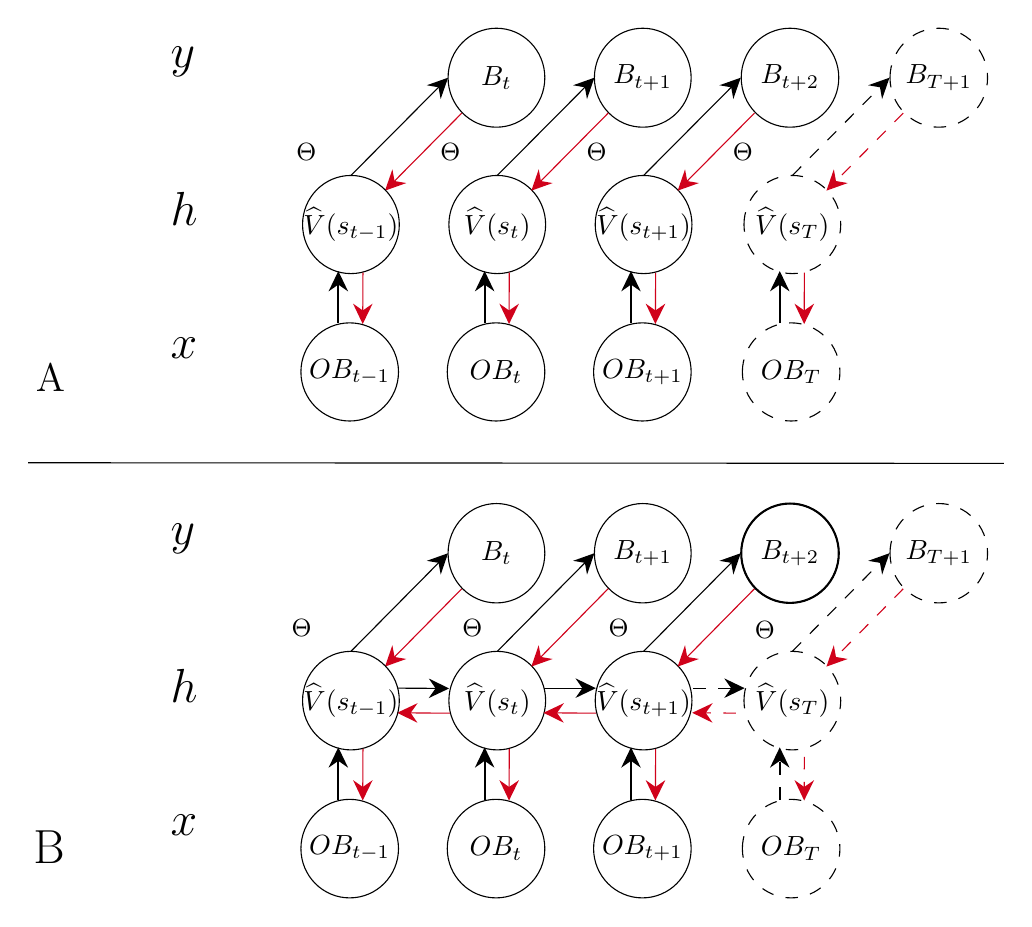
\begin{tikzpicture}[x=0.75pt,y=0.75pt,yscale=-1,xscale=1]
    %uncomment if require: \path (0,432); %set diagram left start at 0, and has height of 432
    
    %Shape: Ellipse [id:dp9152556376471453] 
    \draw   (252.87,325.26) .. controls (252.87,312.15) and (263.3,301.52) .. (276.18,301.52) .. controls (289.05,301.52) and (299.48,312.15) .. (299.48,325.26) .. controls (299.48,338.37) and (289.05,349) .. (276.18,349) .. controls (263.3,349) and (252.87,338.37) .. (252.87,325.26) -- cycle ;
    %Straight Lines [id:da0084456304461753] 
    \draw [color={rgb, 255:red, 208; green, 2; blue, 27 }  ,draw opacity=1 ]   (230.94,331.15) -- (253.32,331.31) ;
    \draw [shift={(227.94,331.12)}, rotate = 0.43] [fill={rgb, 255:red, 208; green, 2; blue, 27 }  ,fill opacity=1 ][line width=0.08]  [draw opacity=0] (9.82,-4.72) -- (0,0) -- (9.82,4.72) -- (6.52,0) -- cycle    ;
    %Shape: Ellipse [id:dp18326344407352502] 
    \draw   (181.58,396.56) .. controls (181.58,383.45) and (192.11,372.82) .. (205.08,372.82) .. controls (218.06,372.82) and (228.59,383.45) .. (228.59,396.56) .. controls (228.59,409.67) and (218.06,420.3) .. (205.08,420.3) .. controls (192.11,420.3) and (181.58,409.67) .. (181.58,396.56) -- cycle ;
    %Shape: Ellipse [id:dp4732045107682973] 
    \draw   (252.09,396.56) .. controls (252.09,383.45) and (262.61,372.82) .. (275.59,372.82) .. controls (288.57,372.82) and (299.09,383.45) .. (299.09,396.56) .. controls (299.09,409.67) and (288.57,420.3) .. (275.59,420.3) .. controls (262.61,420.3) and (252.09,409.67) .. (252.09,396.56) -- cycle ;
    %Straight Lines [id:da9106304988340169] 
    \draw    (205.67,301.52) -- (250.37,256.37) ;
    \draw [shift={(252.48,254.24)}, rotate = 494.71] [fill={rgb, 255:red, 0; green, 0; blue, 0 }  ][line width=0.08]  [draw opacity=0] (9.82,-4.72) -- (0,0) -- (9.82,4.72) -- (6.52,0) -- cycle    ;
    %Straight Lines [id:da5186602107869037] 
    \draw [color={rgb, 255:red, 208; green, 2; blue, 27 }  ,draw opacity=1 ]   (259.09,271.36) -- (224.2,306.73) ;
    \draw [shift={(222.1,308.86)}, rotate = 314.62] [fill={rgb, 255:red, 208; green, 2; blue, 27 }  ,fill opacity=1 ][line width=0.08]  [draw opacity=0] (9.82,-4.72) -- (0,0) -- (9.82,4.72) -- (6.52,0) -- cycle    ;
    %Shape: Ellipse [id:dp6434768624828036] 
    \draw   (322.59,396.56) .. controls (322.59,383.45) and (333.11,372.82) .. (346.09,372.82) .. controls (359.07,372.82) and (369.59,383.45) .. (369.59,396.56) .. controls (369.59,409.67) and (359.07,420.3) .. (346.09,420.3) .. controls (333.11,420.3) and (322.59,409.67) .. (322.59,396.56) -- cycle ;
    %Shape: Ellipse [id:dp4847846412537088] 
    \draw   (252.48,254.24) .. controls (252.48,241.02) and (262.91,230.3) .. (275.78,230.3) .. controls (288.65,230.3) and (299.09,241.02) .. (299.09,254.24) .. controls (299.09,267.46) and (288.65,278.18) .. (275.78,278.18) .. controls (262.91,278.18) and (252.48,267.46) .. (252.48,254.24) -- cycle ;
    %Shape: Ellipse [id:dp07973567399208026] 
    \draw   (322.98,254.24) .. controls (322.98,241.02) and (333.42,230.3) .. (346.29,230.3) .. controls (359.16,230.3) and (369.59,241.02) .. (369.59,254.24) .. controls (369.59,267.46) and (359.16,278.18) .. (346.29,278.18) .. controls (333.42,278.18) and (322.98,267.46) .. (322.98,254.24) -- cycle ;
    %Shape: Ellipse [id:dp05423142626898558] 
    \draw   (393.72,254.24) .. controls (393.72,241.02) and (404.24,230.3) .. (417.22,230.3) .. controls (430.2,230.3) and (440.72,241.02) .. (440.72,254.24) .. controls (440.72,267.46) and (430.2,278.18) .. (417.22,278.18) .. controls (404.24,278.18) and (393.72,267.46) .. (393.72,254.24) -- cycle ;
    %Shape: Ellipse [id:dp22782348689960996] 
    \draw   (182.37,325.26) .. controls (182.37,312.15) and (192.8,301.52) .. (205.67,301.52) .. controls (218.54,301.52) and (228.98,312.15) .. (228.98,325.26) .. controls (228.98,338.37) and (218.54,349) .. (205.67,349) .. controls (192.8,349) and (182.37,338.37) .. (182.37,325.26) -- cycle ;
    %Straight Lines [id:da8044112442211012] 
    \draw [line width=0.75]    (270.1,372.91) -- (270.1,350.76) ;
    \draw [shift={(270.1,347.76)}, rotate = 450] [fill={rgb, 255:red, 0; green, 0; blue, 0 }  ][line width=0.08]  [draw opacity=0] (9.82,-4.72) -- (0,0) -- (9.82,4.72) -- (6.52,0) -- cycle    ;
    %Straight Lines [id:da4352361095595384] 
    \draw [color={rgb, 255:red, 208; green, 2; blue, 27 }  ,draw opacity=1 ]   (281.87,370.38) -- (281.97,348.47) ;
    \draw [shift={(281.85,373.38)}, rotate = 270.27] [fill={rgb, 255:red, 208; green, 2; blue, 27 }  ,fill opacity=1 ][line width=0.08]  [draw opacity=0] (9.82,-4.72) -- (0,0) -- (9.82,4.72) -- (6.52,0) -- cycle    ;
    %Straight Lines [id:da9840961706533492] 
    \draw [color={rgb, 255:red, 0; green, 0; blue, 0 }  ,draw opacity=1 ]   (228.41,319.25) -- (249.98,319.36) ;
    \draw [shift={(252.98,319.38)}, rotate = 180.28] [fill={rgb, 255:red, 0; green, 0; blue, 0 }  ,fill opacity=1 ][line width=0.08]  [draw opacity=0] (9.82,-4.72) -- (0,0) -- (9.82,4.72) -- (6.52,0) -- cycle    ;
    %Straight Lines [id:da9105454079139469] 
    \draw [line width=0.75]    (340.61,372.91) -- (340.61,350.76) ;
    \draw [shift={(340.61,347.76)}, rotate = 450] [fill={rgb, 255:red, 0; green, 0; blue, 0 }  ][line width=0.08]  [draw opacity=0] (9.82,-4.72) -- (0,0) -- (9.82,4.72) -- (6.52,0) -- cycle    ;
    %Straight Lines [id:da2563913907740285] 
    \draw [color={rgb, 255:red, 208; green, 2; blue, 27 }  ,draw opacity=1 ]   (352.37,370.38) -- (352.48,348.47) ;
    \draw [shift={(352.36,373.38)}, rotate = 270.27] [fill={rgb, 255:red, 208; green, 2; blue, 27 }  ,fill opacity=1 ][line width=0.08]  [draw opacity=0] (9.82,-4.72) -- (0,0) -- (9.82,4.72) -- (6.52,0) -- cycle    ;
    %Shape: Ellipse [id:dp3682545800349367] 
    \draw   (323.37,325.26) .. controls (323.37,312.15) and (333.81,301.52) .. (346.68,301.52) .. controls (359.55,301.52) and (369.98,312.15) .. (369.98,325.26) .. controls (369.98,338.37) and (359.55,349) .. (346.68,349) .. controls (333.81,349) and (323.37,338.37) .. (323.37,325.26) -- cycle ;
    %Straight Lines [id:da5491729665822646] 
    \draw [line width=0.75]    (199.6,372.91) -- (199.6,350.76) ;
    \draw [shift={(199.6,347.76)}, rotate = 450] [fill={rgb, 255:red, 0; green, 0; blue, 0 }  ][line width=0.08]  [draw opacity=0] (9.82,-4.72) -- (0,0) -- (9.82,4.72) -- (6.52,0) -- cycle    ;
    %Straight Lines [id:da6906936296691885] 
    \draw [color={rgb, 255:red, 208; green, 2; blue, 27 }  ,draw opacity=1 ]   (211.37,370.38) -- (211.47,348.47) ;
    \draw [shift={(211.35,373.38)}, rotate = 270.27] [fill={rgb, 255:red, 208; green, 2; blue, 27 }  ,fill opacity=1 ][line width=0.08]  [draw opacity=0] (9.82,-4.72) -- (0,0) -- (9.82,4.72) -- (6.52,0) -- cycle    ;
    %Straight Lines [id:da8976403312606693] 
    \draw [color={rgb, 255:red, 208; green, 2; blue, 27 }  ,draw opacity=1 ]   (301.45,331.15) -- (323.82,331.31) ;
    \draw [shift={(298.45,331.12)}, rotate = 0.43] [fill={rgb, 255:red, 208; green, 2; blue, 27 }  ,fill opacity=1 ][line width=0.08]  [draw opacity=0] (9.82,-4.72) -- (0,0) -- (9.82,4.72) -- (6.52,0) -- cycle    ;
    %Straight Lines [id:da7873502214297404] 
    \draw [color={rgb, 255:red, 0; green, 0; blue, 0 }  ,draw opacity=1 ]   (298.92,319.25) -- (320.69,319.25) ;
    \draw [shift={(323.69,319.25)}, rotate = 180] [fill={rgb, 255:red, 0; green, 0; blue, 0 }  ,fill opacity=1 ][line width=0.08]  [draw opacity=0] (9.82,-4.72) -- (0,0) -- (9.82,4.72) -- (6.52,0) -- cycle    ;
    %Straight Lines [id:da38615546041268245] 
    \draw    (276.18,301.52) -- (320.87,256.37) ;
    \draw [shift={(322.98,254.24)}, rotate = 494.71] [fill={rgb, 255:red, 0; green, 0; blue, 0 }  ][line width=0.08]  [draw opacity=0] (9.82,-4.72) -- (0,0) -- (9.82,4.72) -- (6.52,0) -- cycle    ;
    %Straight Lines [id:da8727709104298054] 
    \draw [color={rgb, 255:red, 208; green, 2; blue, 27 }  ,draw opacity=1 ]   (329.6,271.36) -- (294.71,306.73) ;
    \draw [shift={(292.6,308.86)}, rotate = 314.62] [fill={rgb, 255:red, 208; green, 2; blue, 27 }  ,fill opacity=1 ][line width=0.08]  [draw opacity=0] (9.82,-4.72) -- (0,0) -- (9.82,4.72) -- (6.52,0) -- cycle    ;
    %Straight Lines [id:da025606451942667974] 
    \draw    (346.68,301.52) -- (391.37,256.37) ;
    \draw [shift={(393.48,254.24)}, rotate = 494.71] [fill={rgb, 255:red, 0; green, 0; blue, 0 }  ][line width=0.08]  [draw opacity=0] (9.82,-4.72) -- (0,0) -- (9.82,4.72) -- (6.52,0) -- cycle    ;
    %Straight Lines [id:da7157498693904918] 
    \draw [color={rgb, 255:red, 208; green, 2; blue, 27 }  ,draw opacity=1 ]   (400.1,271.36) -- (365.21,306.73) ;
    \draw [shift={(363.1,308.86)}, rotate = 314.62] [fill={rgb, 255:red, 208; green, 2; blue, 27 }  ,fill opacity=1 ][line width=0.08]  [draw opacity=0] (9.82,-4.72) -- (0,0) -- (9.82,4.72) -- (6.52,0) -- cycle    ;
    %Shape: Ellipse [id:dp1944088973906778] 
    \draw   (252.87,95.88) .. controls (252.87,82.82) and (263.3,72.23) .. (276.18,72.23) .. controls (289.05,72.23) and (299.48,82.82) .. (299.48,95.88) .. controls (299.48,108.94) and (289.05,119.52) .. (276.18,119.52) .. controls (263.3,119.52) and (252.87,108.94) .. (252.87,95.88) -- cycle ;
    %Shape: Ellipse [id:dp7540301212468546] 
    \draw   (181.58,166.89) .. controls (181.58,153.83) and (192.11,143.25) .. (205.08,143.25) .. controls (218.06,143.25) and (228.59,153.83) .. (228.59,166.89) .. controls (228.59,179.95) and (218.06,190.54) .. (205.08,190.54) .. controls (192.11,190.54) and (181.58,179.95) .. (181.58,166.89) -- cycle ;
    %Shape: Ellipse [id:dp5780436923676984] 
    \draw   (252.09,166.89) .. controls (252.09,153.83) and (262.61,143.25) .. (275.59,143.25) .. controls (288.57,143.25) and (299.09,153.83) .. (299.09,166.89) .. controls (299.09,179.95) and (288.57,190.54) .. (275.59,190.54) .. controls (262.61,190.54) and (252.09,179.95) .. (252.09,166.89) -- cycle ;
    %Straight Lines [id:da6776717368806907] 
    \draw    (205.67,72.23) -- (250.36,27.27) ;
    \draw [shift={(252.48,25.14)}, rotate = 494.83] [fill={rgb, 255:red, 0; green, 0; blue, 0 }  ][line width=0.08]  [draw opacity=0] (9.82,-4.72) -- (0,0) -- (9.82,4.72) -- (6.52,0) -- cycle    ;
    %Straight Lines [id:da030655313121066063] 
    \draw [color={rgb, 255:red, 208; green, 2; blue, 27 }  ,draw opacity=1 ]   (259.09,42.2) -- (224.21,77.42) ;
    \draw [shift={(222.1,79.55)}, rotate = 314.73] [fill={rgb, 255:red, 208; green, 2; blue, 27 }  ,fill opacity=1 ][line width=0.08]  [draw opacity=0] (9.82,-4.72) -- (0,0) -- (9.82,4.72) -- (6.52,0) -- cycle    ;
    %Shape: Ellipse [id:dp9167477381870462] 
    \draw   (322.59,166.89) .. controls (322.59,153.83) and (333.11,143.25) .. (346.09,143.25) .. controls (359.07,143.25) and (369.59,153.83) .. (369.59,166.89) .. controls (369.59,179.95) and (359.07,190.54) .. (346.09,190.54) .. controls (333.11,190.54) and (322.59,179.95) .. (322.59,166.89) -- cycle ;
    %Shape: Ellipse [id:dp28076940126490224] 
    \draw   (252.48,25.14) .. controls (252.48,11.97) and (262.91,1.3) .. (275.78,1.3) .. controls (288.65,1.3) and (299.09,11.97) .. (299.09,25.14) .. controls (299.09,38.31) and (288.65,48.98) .. (275.78,48.98) .. controls (262.91,48.98) and (252.48,38.31) .. (252.48,25.14) -- cycle ;
    %Shape: Ellipse [id:dp018136489069107253] 
    \draw   (322.98,25.14) .. controls (322.98,11.97) and (333.42,1.3) .. (346.29,1.3) .. controls (359.16,1.3) and (369.59,11.97) .. (369.59,25.14) .. controls (369.59,38.31) and (359.16,48.98) .. (346.29,48.98) .. controls (333.42,48.98) and (322.98,38.31) .. (322.98,25.14) -- cycle ;
    %Shape: Ellipse [id:dp43337791741971476] 
    \draw   (393.72,25.14) .. controls (393.72,11.97) and (404.24,1.3) .. (417.22,1.3) .. controls (430.2,1.3) and (440.72,11.97) .. (440.72,25.14) .. controls (440.72,38.31) and (430.2,48.98) .. (417.22,48.98) .. controls (404.24,48.98) and (393.72,38.31) .. (393.72,25.14) -- cycle ;
    %Shape: Ellipse [id:dp27462372888763276] 
    \draw   (182.37,95.88) .. controls (182.37,82.82) and (192.8,72.23) .. (205.67,72.23) .. controls (218.54,72.23) and (228.98,82.82) .. (228.98,95.88) .. controls (228.98,108.94) and (218.54,119.52) .. (205.67,119.52) .. controls (192.8,119.52) and (182.37,108.94) .. (182.37,95.88) -- cycle ;
    %Straight Lines [id:da29813692702208516] 
    \draw [line width=0.75]    (270.1,143.33) -- (270.1,121.29) ;
    \draw [shift={(270.1,118.29)}, rotate = 450] [fill={rgb, 255:red, 0; green, 0; blue, 0 }  ][line width=0.08]  [draw opacity=0] (9.82,-4.72) -- (0,0) -- (9.82,4.72) -- (6.52,0) -- cycle    ;
    %Straight Lines [id:da3349478757051123] 
    \draw [color={rgb, 255:red, 208; green, 2; blue, 27 }  ,draw opacity=1 ]   (281.87,140.81) -- (281.97,118.99) ;
    \draw [shift={(281.85,143.81)}, rotate = 270.27] [fill={rgb, 255:red, 208; green, 2; blue, 27 }  ,fill opacity=1 ][line width=0.08]  [draw opacity=0] (9.82,-4.72) -- (0,0) -- (9.82,4.72) -- (6.52,0) -- cycle    ;
    %Straight Lines [id:da9602295578636938] 
    \draw [line width=0.75]    (340.61,143.33) -- (340.61,121.29) ;
    \draw [shift={(340.61,118.29)}, rotate = 450] [fill={rgb, 255:red, 0; green, 0; blue, 0 }  ][line width=0.08]  [draw opacity=0] (9.82,-4.72) -- (0,0) -- (9.82,4.72) -- (6.52,0) -- cycle    ;
    %Straight Lines [id:da63886615565973] 
    \draw [color={rgb, 255:red, 208; green, 2; blue, 27 }  ,draw opacity=1 ]   (352.37,140.81) -- (352.48,118.99) ;
    \draw [shift={(352.36,143.81)}, rotate = 270.27] [fill={rgb, 255:red, 208; green, 2; blue, 27 }  ,fill opacity=1 ][line width=0.08]  [draw opacity=0] (9.82,-4.72) -- (0,0) -- (9.82,4.72) -- (6.52,0) -- cycle    ;
    %Shape: Ellipse [id:dp8361207322156409] 
    \draw   (323.37,95.88) .. controls (323.37,82.82) and (333.81,72.23) .. (346.68,72.23) .. controls (359.55,72.23) and (369.98,82.82) .. (369.98,95.88) .. controls (369.98,108.94) and (359.55,119.52) .. (346.68,119.52) .. controls (333.81,119.52) and (323.37,108.94) .. (323.37,95.88) -- cycle ;
    %Straight Lines [id:da4551016346165171] 
    \draw [line width=0.75]    (199.6,143.33) -- (199.6,121.29) ;
    \draw [shift={(199.6,118.29)}, rotate = 450] [fill={rgb, 255:red, 0; green, 0; blue, 0 }  ][line width=0.08]  [draw opacity=0] (9.82,-4.72) -- (0,0) -- (9.82,4.72) -- (6.52,0) -- cycle    ;
    %Straight Lines [id:da561902479346039] 
    \draw [color={rgb, 255:red, 208; green, 2; blue, 27 }  ,draw opacity=1 ]   (211.37,140.81) -- (211.47,118.99) ;
    \draw [shift={(211.35,143.81)}, rotate = 270.27] [fill={rgb, 255:red, 208; green, 2; blue, 27 }  ,fill opacity=1 ][line width=0.08]  [draw opacity=0] (9.82,-4.72) -- (0,0) -- (9.82,4.72) -- (6.52,0) -- cycle    ;
    %Straight Lines [id:da8478794915247372] 
    \draw    (276.18,72.23) -- (320.87,27.27) ;
    \draw [shift={(322.98,25.14)}, rotate = 494.83] [fill={rgb, 255:red, 0; green, 0; blue, 0 }  ][line width=0.08]  [draw opacity=0] (9.82,-4.72) -- (0,0) -- (9.82,4.72) -- (6.52,0) -- cycle    ;
    %Straight Lines [id:da27798944049873586] 
    \draw [color={rgb, 255:red, 208; green, 2; blue, 27 }  ,draw opacity=1 ]   (329.6,42.2) -- (294.71,77.42) ;
    \draw [shift={(292.6,79.55)}, rotate = 314.73] [fill={rgb, 255:red, 208; green, 2; blue, 27 }  ,fill opacity=1 ][line width=0.08]  [draw opacity=0] (9.82,-4.72) -- (0,0) -- (9.82,4.72) -- (6.52,0) -- cycle    ;
    %Straight Lines [id:da24137509475938523] 
    \draw    (346.68,72.23) -- (391.37,27.27) ;
    \draw [shift={(393.48,25.14)}, rotate = 494.83] [fill={rgb, 255:red, 0; green, 0; blue, 0 }  ][line width=0.08]  [draw opacity=0] (9.82,-4.72) -- (0,0) -- (9.82,4.72) -- (6.52,0) -- cycle    ;
    %Straight Lines [id:da5361482602236827] 
    \draw [color={rgb, 255:red, 208; green, 2; blue, 27 }  ,draw opacity=1 ]   (400.1,42.2) -- (365.21,77.42) ;
    \draw [shift={(363.1,79.55)}, rotate = 314.73] [fill={rgb, 255:red, 208; green, 2; blue, 27 }  ,fill opacity=1 ][line width=0.08]  [draw opacity=0] (9.82,-4.72) -- (0,0) -- (9.82,4.72) -- (6.52,0) -- cycle    ;
    %Shape: Ellipse [id:dp9428082939545759] 
    \draw  [dash pattern={on 4.5pt off 4.5pt}] (394.27,166.89) .. controls (394.27,153.83) and (404.79,143.25) .. (417.77,143.25) .. controls (430.75,143.25) and (441.27,153.83) .. (441.27,166.89) .. controls (441.27,179.95) and (430.75,190.54) .. (417.77,190.54) .. controls (404.79,190.54) and (394.27,179.95) .. (394.27,166.89) -- cycle ;
    %Shape: Ellipse [id:dp12638273249032017] 
    \draw  [dash pattern={on 4.5pt off 4.5pt}] (465.4,25.14) .. controls (465.4,11.97) and (475.92,1.3) .. (488.9,1.3) .. controls (501.88,1.3) and (512.4,11.97) .. (512.4,25.14) .. controls (512.4,38.31) and (501.88,48.98) .. (488.9,48.98) .. controls (475.92,48.98) and (465.4,38.31) .. (465.4,25.14) -- cycle ;
    %Shape: Ellipse [id:dp8917959348395956] 
    \draw  [dash pattern={on 4.5pt off 4.5pt}] (395.05,95.88) .. controls (395.05,82.82) and (405.49,72.23) .. (418.36,72.23) .. controls (431.23,72.23) and (441.66,82.82) .. (441.66,95.88) .. controls (441.66,108.94) and (431.23,119.52) .. (418.36,119.52) .. controls (405.49,119.52) and (395.05,108.94) .. (395.05,95.88) -- cycle ;
    %Straight Lines [id:da6091521843857648] 
    \draw  [dash pattern={on 4.5pt off 4.5pt}]  (418.36,72.23) -- (463.05,27.27) ;
    \draw [shift={(465.16,25.14)}, rotate = 494.83] [fill={rgb, 255:red, 0; green, 0; blue, 0 }  ][line width=0.08]  [draw opacity=0] (9.82,-4.72) -- (0,0) -- (9.82,4.72) -- (6.52,0) -- cycle    ;
    %Straight Lines [id:da18105258004250324] 
    \draw [color={rgb, 255:red, 208; green, 2; blue, 27 }  ,draw opacity=1 ] [dash pattern={on 4.5pt off 4.5pt}]  (471.78,42.2) -- (436.89,77.42) ;
    \draw [shift={(434.78,79.55)}, rotate = 314.73] [fill={rgb, 255:red, 208; green, 2; blue, 27 }  ,fill opacity=1 ][line width=0.08]  [draw opacity=0] (9.82,-4.72) -- (0,0) -- (9.82,4.72) -- (6.52,0) -- cycle    ;
    %Straight Lines [id:da6760788428742098] 
    \draw [line width=0.75]    (412.29,143.33) -- (412.29,121.29) ;
    \draw [shift={(412.29,118.29)}, rotate = 450] [fill={rgb, 255:red, 0; green, 0; blue, 0 }  ][line width=0.08]  [draw opacity=0] (9.82,-4.72) -- (0,0) -- (9.82,4.72) -- (6.52,0) -- cycle    ;
    %Straight Lines [id:da7825592771106329] 
    \draw [color={rgb, 255:red, 208; green, 2; blue, 27 }  ,draw opacity=1 ]   (424.05,140.81) -- (424.15,118.99) ;
    \draw [shift={(424.04,143.81)}, rotate = 270.27] [fill={rgb, 255:red, 208; green, 2; blue, 27 }  ,fill opacity=1 ][line width=0.08]  [draw opacity=0] (9.82,-4.72) -- (0,0) -- (9.82,4.72) -- (6.52,0) -- cycle    ;
    %Shape: Ellipse [id:dp44556831775872074] 
    \draw  [line width=0.75]  (393.72,254.24) .. controls (393.72,241.02) and (404.24,230.3) .. (417.22,230.3) .. controls (430.2,230.3) and (440.72,241.02) .. (440.72,254.24) .. controls (440.72,267.46) and (430.2,278.18) .. (417.22,278.18) .. controls (404.24,278.18) and (393.72,267.46) .. (393.72,254.24) -- cycle ;
    %Shape: Ellipse [id:dp001475416847050881] 
    \draw  [dash pattern={on 4.5pt off 4.5pt}] (394.27,396.56) .. controls (394.27,383.45) and (404.79,372.82) .. (417.77,372.82) .. controls (430.75,372.82) and (441.27,383.45) .. (441.27,396.56) .. controls (441.27,409.67) and (430.75,420.3) .. (417.77,420.3) .. controls (404.79,420.3) and (394.27,409.67) .. (394.27,396.56) -- cycle ;
    %Shape: Ellipse [id:dp6004502309758961] 
    \draw  [dash pattern={on 4.5pt off 4.5pt}] (465.4,254.24) .. controls (465.4,241.02) and (475.92,230.3) .. (488.9,230.3) .. controls (501.88,230.3) and (512.4,241.02) .. (512.4,254.24) .. controls (512.4,267.46) and (501.88,278.18) .. (488.9,278.18) .. controls (475.92,278.18) and (465.4,267.46) .. (465.4,254.24) -- cycle ;
    %Shape: Ellipse [id:dp9012578897389621] 
    \draw  [dash pattern={on 4.5pt off 4.5pt}] (395.05,325.26) .. controls (395.05,312.15) and (405.49,301.52) .. (418.36,301.52) .. controls (431.23,301.52) and (441.66,312.15) .. (441.66,325.26) .. controls (441.66,338.37) and (431.23,349) .. (418.36,349) .. controls (405.49,349) and (395.05,338.37) .. (395.05,325.26) -- cycle ;
    %Straight Lines [id:da8776948176349402] 
    \draw  [dash pattern={on 4.5pt off 4.5pt}]  (418.36,301.52) -- (463.05,256.37) ;
    \draw [shift={(465.16,254.24)}, rotate = 494.71] [fill={rgb, 255:red, 0; green, 0; blue, 0 }  ][line width=0.08]  [draw opacity=0] (9.82,-4.72) -- (0,0) -- (9.82,4.72) -- (6.52,0) -- cycle    ;
    %Straight Lines [id:da11237121474720091] 
    \draw [color={rgb, 255:red, 208; green, 2; blue, 27 }  ,draw opacity=1 ] [dash pattern={on 4.5pt off 4.5pt}]  (471.78,271.36) -- (436.89,306.73) ;
    \draw [shift={(434.78,308.86)}, rotate = 314.62] [fill={rgb, 255:red, 208; green, 2; blue, 27 }  ,fill opacity=1 ][line width=0.08]  [draw opacity=0] (9.82,-4.72) -- (0,0) -- (9.82,4.72) -- (6.52,0) -- cycle    ;
    %Straight Lines [id:da12172698001213589] 
    \draw [line width=0.75]  [dash pattern={on 4.5pt off 4.5pt}]  (412.29,372.91) -- (412.29,350.76) ;
    \draw [shift={(412.29,347.76)}, rotate = 450] [fill={rgb, 255:red, 0; green, 0; blue, 0 }  ][line width=0.08]  [draw opacity=0] (9.82,-4.72) -- (0,0) -- (9.82,4.72) -- (6.52,0) -- cycle    ;
    %Straight Lines [id:da6444397198631048] 
    \draw [color={rgb, 255:red, 208; green, 2; blue, 27 }  ,draw opacity=1 ] [dash pattern={on 4.5pt off 4.5pt}]  (424.05,370.38) -- (424.15,348.47) ;
    \draw [shift={(424.04,373.38)}, rotate = 270.27] [fill={rgb, 255:red, 208; green, 2; blue, 27 }  ,fill opacity=1 ][line width=0.08]  [draw opacity=0] (9.82,-4.72) -- (0,0) -- (9.82,4.72) -- (6.52,0) -- cycle    ;
    %Straight Lines [id:da11944678601617786] 
    \draw [color={rgb, 255:red, 208; green, 2; blue, 27 }  ,draw opacity=1 ] [dash pattern={on 4.5pt off 4.5pt}]  (373.12,331.15) -- (395.5,331.31) ;
    \draw [shift={(370.12,331.12)}, rotate = 0.43] [fill={rgb, 255:red, 208; green, 2; blue, 27 }  ,fill opacity=1 ][line width=0.08]  [draw opacity=0] (9.82,-4.72) -- (0,0) -- (9.82,4.72) -- (6.52,0) -- cycle    ;
    %Straight Lines [id:da6070445313661826] 
    \draw [color={rgb, 255:red, 0; green, 0; blue, 0 }  ,draw opacity=1 ] [dash pattern={on 4.5pt off 4.5pt}]  (370.59,319.25) -- (392.36,319.25) ;
    \draw [shift={(395.36,319.25)}, rotate = 180] [fill={rgb, 255:red, 0; green, 0; blue, 0 }  ,fill opacity=1 ][line width=0.08]  [draw opacity=0] (9.82,-4.72) -- (0,0) -- (9.82,4.72) -- (6.52,0) -- cycle    ;
    %Straight Lines [id:da8091605227382529] 
    \draw    (50.2,210.65) -- (520.2,210.95) ;
    
    % Text Node
    \draw (51.39,386.85) node [anchor=north west][inner sep=0.75pt]   [align=left] {{\LARGE B}};
    % Text Node
    \draw (205.08,396.56) node    {$OB_{t-1}$};
    % Text Node
    \draw (205.67,325.26) node    {$\widehat{V}(s_{t-1})$};
    % Text Node
    \draw (275.59,396.56) node    {$OB_{t}$};
    % Text Node
    \draw (276.18,325.26) node    {$\widehat{V}(s_t)$};
    % Text Node
    \draw (275.78,254.24) node    {$B_{t}$};
    % Text Node
    \draw (346.09,396.56) node  [font=\normalsize]  {$OB_{t+1}$};
    % Text Node
    \draw (346.68,325.26) node    {$\widehat{V}(s_{t+1})$};
    % Text Node
    \draw (346.29,254.24) node    {$B_{t+1}$};
    % Text Node
    \draw (417.22,254.24) node    {$B_{t+2}$};
    % Text Node
    \draw (181.86,290.07) node  [font=\small]  {$\Theta$};
    % Text Node
    \draw (264.11,290.07) node  [font=\small]  {$\Theta$};
    % Text Node
    \draw (334.61,290.07) node  [font=\small]  {$\Theta$};
    % Text Node
    \draw (205.08,166.89) node    {$OB_{t-1}$};
    % Text Node
    \draw (205.67,95.88) node    {$\widehat{V}(s_{t-1})$};
    % Text Node
    \draw (275.59,166.89) node    {$OB_{t}$};
    % Text Node
    \draw (276.18,95.88) node    {$\widehat{V}(s_{t})$};
    % Text Node
    \draw (275.78,25.14) node    {$B_{t}$};
    % Text Node
    \draw (346.09,166.89) node    {$OB_{t+1}$};
    % Text Node
    \draw (346.68,95.88) node    {$\widehat{V}(s_{t+1})$};
    % Text Node
    \draw (346.29,25.14) node    {$B_{t+1}$};
    % Text Node
    \draw (417.22,25.14) node    {$B_{t+2}$};
    % Text Node
    \draw (184.21,60.83) node  [font=\small]  {$\Theta $};
    % Text Node
    \draw (417.77,166.89) node    {$OB_{T}$};
    % Text Node
    \draw (418.36,95.88) node    {$\widehat{V}(s_{T})$};
    % Text Node
    \draw (488.9,25.14) node    {$B_{T+1}$};
    % Text Node
    \draw (52.57,162.08) node [anchor=north west][inner sep=0.75pt]   [align=left] {{\Large A}};
    % Text Node
    \draw (417.77,396.56) node    {$OB_{T}$};
    % Text Node
    \draw (418.36,325.26) node    {$\widehat{V}(s_{T})$};
    % Text Node
    \draw (488.9,254.24) node    {$B_{T+1}$};
    % Text Node
    \draw (405.12,291.26) node  [font=\small]  {$\Theta$};
    % Text Node
    \draw (253.54,60.83) node  [font=\small]  {$\Theta$};
    % Text Node
    \draw (324.04,60.83) node  [font=\small]  {$\Theta$};
    % Text Node
    \draw (394.54,60.83) node  [font=\small]  {$\Theta$};
    % Text Node
    \draw (117.57,9.08) node [anchor=north west][inner sep=0.75pt]  [font=\LARGE] [align=left] {$\displaystyle y$};
    % Text Node
    \draw (117.57,79.08) node [anchor=north west][inner sep=0.75pt]  [font=\LARGE] [align=left] {$\displaystyle h$};
    % Text Node
    \draw (117.57,149.08) node [anchor=north west][inner sep=0.75pt]  [font=\LARGE] [align=left] {$\displaystyle x$};
    % Text Node
    \draw (117.57,239.08) node [anchor=north west][inner sep=0.75pt]  [font=\LARGE] [align=left] {$\displaystyle y$};
    % Text Node
    \draw (117.57,309.08) node [anchor=north west][inner sep=0.75pt]  [font=\LARGE] [align=left] {$\displaystyle h$};
    % Text Node
    \draw (117.57,379.08) node [anchor=north west][inner sep=0.75pt]  [font=\LARGE] [align=left] {$\displaystyle x$};

    \end{tikzpicture}
\end{adjustbox}
\end{center}

\caption[\textbf{Differences in single-step prediction between feed-forward and recurrent neural networks}]{ Adapted from \cite{bengio2017deep,lillicrap2019backpropagation}, the figure represents how feedforward and recurrent ANNs could be used for estimating $V(s_t)$. Here $OB=\{OB_{t}: t \in T\}$ indicates the series of inputs of length $T$  that the network receives while the target is the lead 1 version of the $B$ portion of the same series. The series $\widehat{V}=\{\widehat{V}(s_{t}): t \in T\}$ correspond to the representations generated combining the input with the parameters $\Theta$ learned by the network in order to approximate the target. Circles indicate computational blocks similar to those present in figure \ref{fig: ffnn}. Black and red arrows are respectively the direction of the computations and the flow of the error gradient.}
\label{fig: ffnn_rnn}
\end{figure}

\subsection{Artificial Neural Networks for Manifold Learning}
\label{manifold_learning}
As mentioned in the previous sections, ANNs are tasked to create latent representations (e.g. $V(s_{t})$) which are not explicitly defined by their input or target but are nevertheless functional for connecting the two \cite{rumelhart1986learning,bengio2017deep,lillicrap2020backpropagation}. This is based on the hypothesis that the relationship between the input and the target can be expressed in terms of variations in coordinates on a manifold \cite{bengio2017deep}. In the lower dimensional space of this manifold, the input is re-organized to improve estimation and elements which are similar to each other tend to appear close together \cite{bengio2017deep}. In this view, during optimization, each layer of an ANN attempts to place its input on a manifold that is useful for the layer that follows. This process continues until the last layer. Here the inputs are organized in such way that it makes easier for the network to produce good predictions of the target \cite{bengio2017deep}. Moving along this final manifold allows one to reach inputs with different characteristics leading to variations in the predictions produced by the model. We hypothesize that the amount of attributed incentive salience (i.e. $V(s_{t})$) can be modeled as a manifold on which the history of individual-object interactions is placed in order to best predict the intensity of all future interactions. This relates to the concept of motivation as a vector presented in sections \ref{motivation}: the representation $V(s_{t})$ estimated by an ANN can be thought of as a vector in an $h$ dimensional space, where $h$ is the number of units of the layer producing the representation, indicating the amount of attributed incentive salience after observing $t$ interactions. As we can see, differently from completely un-supervised approaches this approach forces the learned manifold to obey to specific representational and predictive functionalities that are shared with the construct of attributed incentive salience. Given the potentially large number of layers in an ANN, locating this representation and most importantly ensuring that it is a suitable approximation of $V(s_{t})$ are potential issues. A possible solution is to impose a form of architectural constraint on the optimization process through multi-task learning. Multi-task learning closely resemble multivariate analysis, it  works on the assumption that a common latent factor underlying a set of targets exists and it can be constrained in a single representation used by the ANN for producing multiple predictions \cite{bengio2017deep}. An example of this process is shown in figure \ref{fig: multi_task}. As mentioned in section \ref{incentive_salience}, the amount of attributed incentive salience $V(s_t)$ that an individual $I$ assigns to an object $O$ should be a latent factor that indicates how intense future interactions with that object will be. Therefore, if a layer in an ANN is forced to produce a single representation which is then used to estimate multiple behavioural indicators of the intensity of these interactions, this should provide a sensible approximation of the amount of attributed incentive salience. 
\begin{figure}[h]
  \begin{center}
    \begin{adjustbox}{width=0.4\columnwidth}
        \tikzset{every picture/.style={line width=0.75pt}} %set default line width to 0.75pt        
        
        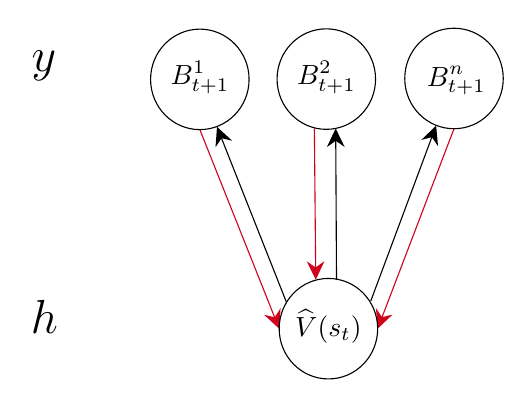
\begin{tikzpicture}[x=0.75pt,y=0.75pt,yscale=-1,xscale=1]
        %uncomment if require: \path (0,300); %set diagram left start at 0, and has height of 300
        
        %Straight Lines [id:da4267952151606098] 
        \draw    (319.82,122) -- (320.2,191.88) ;
        \draw [shift={(319.8,119)}, rotate = 89.69] [fill={rgb, 255:red, 0; green, 0; blue, 0 }  ][line width=0.08]  [draw opacity=0] (8.93,-4.29) -- (0,0) -- (8.93,4.29) -- (5.93,0) -- cycle    ;
        %Straight Lines [id:da6989378371909234] 
        \draw [color={rgb, 255:red, 208; green, 2; blue, 27 }  ,draw opacity=1 ]   (310.17,188.88) -- (309.53,119) ;
        \draw [shift={(310.2,191.88)}, rotate = 269.48] [fill={rgb, 255:red, 208; green, 2; blue, 27 }  ,fill opacity=1 ][line width=0.08]  [draw opacity=0] (8.93,-4.29) -- (0,0) -- (8.93,4.29) -- (5.93,0) -- cycle    ;
        %Shape: Ellipse [id:dp8707618719305075] 
        \draw   (353.08,94.91) .. controls (353.08,81.53) and (363.7,70.7) .. (376.81,70.7) .. controls (389.91,70.7) and (400.53,81.53) .. (400.53,94.91) .. controls (400.53,108.28) and (389.91,119.12) .. (376.81,119.12) .. controls (363.7,119.12) and (353.08,108.28) .. (353.08,94.91) -- cycle ;
        %Straight Lines [id:da13933094112344846] 
        \draw [color={rgb, 255:red, 208; green, 2; blue, 27 }  ,draw opacity=1 ]   (341.1,212.65) -- (376.81,119.12) ;
        \draw [shift={(340.03,215.46)}, rotate = 290.89] [fill={rgb, 255:red, 208; green, 2; blue, 27 }  ,fill opacity=1 ][line width=0.08]  [draw opacity=0] (8.93,-4.29) -- (0,0) -- (8.93,4.29) -- (5.93,0) -- cycle    ;
        %Shape: Ellipse [id:dp9097319337144372] 
        \draw   (291.56,95.2) .. controls (291.56,81.82) and (302.18,70.99) .. (315.29,70.99) .. controls (328.39,70.99) and (339.01,81.82) .. (339.01,95.2) .. controls (339.01,108.57) and (328.39,119.41) .. (315.29,119.41) .. controls (302.18,119.41) and (291.56,108.57) .. (291.56,95.2) -- cycle ;
        %Straight Lines [id:da3769355222150532] 
        \draw [color={rgb, 255:red, 208; green, 2; blue, 27 }  ,draw opacity=1 ]   (291.47,212.67) -- (254.35,119.55) ;
        \draw [shift={(292.58,215.46)}, rotate = 248.27] [fill={rgb, 255:red, 208; green, 2; blue, 27 }  ,fill opacity=1 ][line width=0.08]  [draw opacity=0] (8.93,-4.29) -- (0,0) -- (8.93,4.29) -- (5.93,0) -- cycle    ;
        %Straight Lines [id:da1253267073766362] 
        \draw [color={rgb, 255:red, 0; green, 0; blue, 0 }  ,draw opacity=1 ]   (263.71,120.96) -- (296.02,202.56) ;
        \draw [shift={(262.61,118.17)}, rotate = 68.4] [fill={rgb, 255:red, 0; green, 0; blue, 0 }  ,fill opacity=1 ][line width=0.08]  [draw opacity=0] (8.93,-4.29) -- (0,0) -- (8.93,4.29) -- (5.93,0) -- cycle    ;
        %Shape: Ellipse [id:dp7350394708339132] 
        \draw   (292.58,215.46) .. controls (292.58,202.09) and (303.2,191.25) .. (316.3,191.25) .. controls (329.41,191.25) and (340.03,202.09) .. (340.03,215.46) .. controls (340.03,228.83) and (329.41,239.67) .. (316.3,239.67) .. controls (303.2,239.67) and (292.58,228.83) .. (292.58,215.46) -- cycle ;
        %Shape: Ellipse [id:dp34753658855295044] 
        \draw   (230.62,95.34) .. controls (230.62,81.97) and (241.24,71.13) .. (254.35,71.13) .. controls (267.45,71.13) and (278.07,81.97) .. (278.07,95.34) .. controls (278.07,108.71) and (267.45,119.55) .. (254.35,119.55) .. controls (241.24,119.55) and (230.62,108.71) .. (230.62,95.34) -- cycle ;
        %Straight Lines [id:da6916637423351373] 
        \draw [color={rgb, 255:red, 0; green, 0; blue, 0 }  ,draw opacity=1 ]   (367.15,120.44) -- (336.7,202.13) ;
        \draw [shift={(368.2,117.63)}, rotate = 110.44] [fill={rgb, 255:red, 0; green, 0; blue, 0 }  ,fill opacity=1 ][line width=0.08]  [draw opacity=0] (8.93,-4.29) -- (0,0) -- (8.93,4.29) -- (5.93,0) -- cycle    ;
        
        % Text Node
        \draw (316.33,214.5) node   [align=left] {$\displaystyle \widehat{V}( s_{t})$};
        % Text Node
        \draw (254.43,94.4) node   [align=left] {$\displaystyle B^{1}_{t+1}$};
        % Text Node
        \draw (315.37,94.25) node   [align=left] {$\displaystyle B^{2}_{t+1}$};
        % Text Node
        \draw (377.91,95.99) node   [align=left] {$\displaystyle B^{n}_{t+1}$};
        % Text Node
        \draw (171.67,200.4) node [anchor=north west][inner sep=0.75pt]  [font=\LARGE]  {$h$};
        % Text Node
        \draw (172,80.4) node [anchor=north west][inner sep=0.75pt]  [font=\LARGE]  {$y$};
        
        \end{tikzpicture}
    \end{adjustbox}
\end{center}
\caption[\textbf{Multi-task learning}]{Adapted from \cite{bengio2017deep}. The figure represents how multi-task learning could be used in an ANN to force the the latent representation $h$ to be a sensible approximation of $V(s_t)$. Here $\widehat{V}(s_t)$ indicates the representation generated by a recurrent layer at time $t$ while $B_{t+1}=\{B^n_{t+1}: n \in N\}$ are $N$ targets quantifying the strength of the next interaction (in terms of frequency and amount of behaviour)  between $I$ and $O$. Black and red arrows are respectively the direction of the computations and the flow of the error gradient. Circles indicate computational blocks similar to those in figures \ref{fig: ffnn} and \ref{fig: ffnn_rnn}.}
\label{fig: multi_task}
\end{figure}

\subsection{Modelling the contribution of Game Events and Environment Indicators}
\label{modelling_env_and_game_elements}
As we mentioned in chapter \ref{chapter_lit_review}, the current ammount of attributed incentive salience is in part conditioned by the characteristics of the game while its behavioural manifestation can be affected by the environment surrounding the individual. These two factors are not taken into consideration in the modelling framework we just proposed, indeed we assume them to be absorbed, to a certain extent, by the behavioural indicator $B$. If the game characteristics are not able to provide sufficient rewarding experiences or some environmental factors act as an impediment, we can expect to observe less intense and frequent interactions between $I$ and $O$. However in this setting it would be hard to disentangle which factors contributed to the reduction in observed behaviour: was it due to a long-running decline in the level of attributed incentive salience or to an unfavourable conjunction of in-game and out-game events? In this view introducing historical information about the interaction than an individual had with particular characterisitcs of the game object and the environmental context in which they occurred should not just improve the prediction of $\widehat{B}_{t+1}$ but also the estimation of $\widehat{V}(s_t)$. Of course introducing and modelling an extra set of predictors in an ANN is relatively straightforward and increasing the number of available parameters should help incorporating the additional information, however this would make the interpretation of the derived latent representation even more challenging. A possible solution to this problem is to modify the architecture of the ANN in order to integrate the addtional information in a similar way to what Generalized Additive Model (GAM) would do \cite{hastie2017generalized}. Solving the problem of predicting $B_{t+1}$ within a GAM framework for a single game object could have the following formulation:
\begin{gather}
\label{gam}
    \widehat{B}_{t+1} = \beta + f^{B}(B_{t:t-n};\theta^{B}) + f^{G}(G_{t:t-n};\theta^{G}) + f^{Env}(Env_{t:t-n};\theta^{Env})
\end{gather}
here $\beta$ is a generic intercept while $B_{t:t-n}$, $G_{t:t-n}$ and $Env_{t:t-n}$ are temporal series of behavioural metrics, game events and environment indicators up to time $t$. The corresponding functions $f^{B}$, $f^{G}$ and $f^{Env}$ are usually linear or non linear (e.g. splines) additive models. The framework offered by GAM is a good compromise between complexity and explainability as it allows to consider many predictors while enforcing a structural form that makes the function associated to each of them directly interpretable \cite{hastie2017generalized}. In a work by Agarwal et al. \cite{agarwal2021neural} the authors extended the GAM framework to ANN (Neural Addtive Models, NAM), the general idea behind this is to substitute each function expressed in equation \ref{gam} with an appropriated ANN and to derive the prediction of the model as a linear combination of them. The additive nature of NAM, despite posing a constrain on how each function gets integrated with the others, makes it possible to know exactly how each function contribute to the final prediction \cite{hastie2017generalized,agarwal2017quitting}. In our setting we are less interested in retrieving the exact functional form associated to any of the three sources of information (i.e. behaviour, game characteristics and environment) and more in being able to generate separable representations for each one of them. In this view, combining the functional form of equation \ref{gam} with the ideas presented in this chapter we could formulate the estimation of $V(s_t)$ as a non-linear combination of separate functions (all parametrized by ANNs) and subsequently use this for predicting $B_{t+1}$
\begin{gather}
\label{nam}
    \widehat{B_t} = f^{B}(B_{t:t-n}, O;\theta^{B}) \\
    \widehat{G_t} = f^{G}(G_{t:t-n}, O;\theta^{G}) \\ 
    \widehat{Env_t} = f^{Env}(Env_{t:t-n}, O;\theta^{Env}) \\
    \widehat{V}(s_t) = f^{V}(B_t, G_t, Env_t; \theta^{V})
\end{gather}
here $\widehat{B_t}$, $\widehat{G_t}$, $\widehat{Env_t}$ and $\widehat{V}(s_t)$ are representation generated by the respective functions $f$. Each function can be though as being parametrized by a recurrent ANN as specified in section \ref{rnn_theory}. The final representation $\widehat{V}(s_t)$ would then be used for solving the same type of multi-task learning problem presented in section \ref{manifold_learning}. A graphic representation for this can be found in figure \ref{fig: nam_multi_task}.
\begin{figure}
    \begin{center}
        \begin{adjustbox}{width=0.4\textwidth}

            \tikzset{every picture/.style={line width=0.75pt}} %set default line width to 0.75pt        
            
            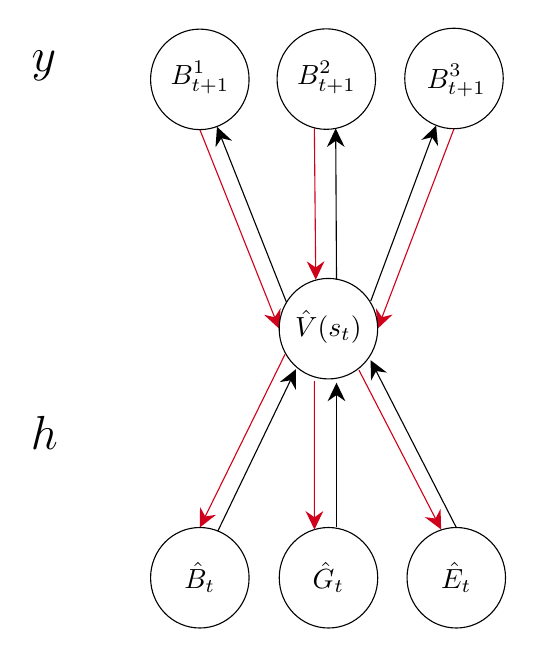
\begin{tikzpicture}[x=0.75pt,y=0.75pt,yscale=-1,xscale=1]
            %uncomment if require: \path (0,488); %set diagram left start at 0, and has height of 488
            
            %Straight Lines [id:da4267952151606098] 
            \draw    (319.82,122) -- (320.2,191.88) ;
            \draw [shift={(319.8,119)}, rotate = 89.69] [fill={rgb, 255:red, 0; green, 0; blue, 0 }  ][line width=0.08]  [draw opacity=0] (8.93,-4.29) -- (0,0) -- (8.93,4.29) -- (5.93,0) -- cycle    ;
            %Straight Lines [id:da6989378371909234] 
            \draw [color={rgb, 255:red, 208; green, 2; blue, 27 }  ,draw opacity=1 ]   (310.17,188.88) -- (309.53,119) ;
            \draw [shift={(310.2,191.88)}, rotate = 269.48] [fill={rgb, 255:red, 208; green, 2; blue, 27 }  ,fill opacity=1 ][line width=0.08]  [draw opacity=0] (8.93,-4.29) -- (0,0) -- (8.93,4.29) -- (5.93,0) -- cycle    ;
            %Shape: Ellipse [id:dp8707618719305075] 
            \draw   (353.08,94.91) .. controls (353.08,81.53) and (363.7,70.7) .. (376.81,70.7) .. controls (389.91,70.7) and (400.53,81.53) .. (400.53,94.91) .. controls (400.53,108.28) and (389.91,119.12) .. (376.81,119.12) .. controls (363.7,119.12) and (353.08,108.28) .. (353.08,94.91) -- cycle ;
            %Straight Lines [id:da13933094112344846] 
            \draw [color={rgb, 255:red, 208; green, 2; blue, 27 }  ,draw opacity=1 ]   (341.1,212.65) -- (376.81,119.12) ;
            \draw [shift={(340.03,215.46)}, rotate = 290.89] [fill={rgb, 255:red, 208; green, 2; blue, 27 }  ,fill opacity=1 ][line width=0.08]  [draw opacity=0] (8.93,-4.29) -- (0,0) -- (8.93,4.29) -- (5.93,0) -- cycle    ;
            %Shape: Ellipse [id:dp9097319337144372] 
            \draw   (291.56,95.2) .. controls (291.56,81.82) and (302.18,70.99) .. (315.29,70.99) .. controls (328.39,70.99) and (339.01,81.82) .. (339.01,95.2) .. controls (339.01,108.57) and (328.39,119.41) .. (315.29,119.41) .. controls (302.18,119.41) and (291.56,108.57) .. (291.56,95.2) -- cycle ;
            %Straight Lines [id:da3769355222150532] 
            \draw [color={rgb, 255:red, 208; green, 2; blue, 27 }  ,draw opacity=1 ]   (291.47,212.67) -- (254.35,119.55) ;
            \draw [shift={(292.58,215.46)}, rotate = 248.27] [fill={rgb, 255:red, 208; green, 2; blue, 27 }  ,fill opacity=1 ][line width=0.08]  [draw opacity=0] (8.93,-4.29) -- (0,0) -- (8.93,4.29) -- (5.93,0) -- cycle    ;
            %Straight Lines [id:da1253267073766362] 
            \draw [color={rgb, 255:red, 0; green, 0; blue, 0 }  ,draw opacity=1 ]   (263.71,120.96) -- (296.02,202.56) ;
            \draw [shift={(262.61,118.17)}, rotate = 68.4] [fill={rgb, 255:red, 0; green, 0; blue, 0 }  ,fill opacity=1 ][line width=0.08]  [draw opacity=0] (8.93,-4.29) -- (0,0) -- (8.93,4.29) -- (5.93,0) -- cycle    ;
            %Shape: Ellipse [id:dp7350394708339132] 
            \draw   (292.58,215.46) .. controls (292.58,202.09) and (303.2,191.25) .. (316.3,191.25) .. controls (329.41,191.25) and (340.03,202.09) .. (340.03,215.46) .. controls (340.03,228.83) and (329.41,239.67) .. (316.3,239.67) .. controls (303.2,239.67) and (292.58,228.83) .. (292.58,215.46) -- cycle ;
            %Shape: Ellipse [id:dp34753658855295044] 
            \draw   (230.62,95.34) .. controls (230.62,81.97) and (241.24,71.13) .. (254.35,71.13) .. controls (267.45,71.13) and (278.07,81.97) .. (278.07,95.34) .. controls (278.07,108.71) and (267.45,119.55) .. (254.35,119.55) .. controls (241.24,119.55) and (230.62,108.71) .. (230.62,95.34) -- cycle ;
            %Straight Lines [id:da6916637423351373] 
            \draw [color={rgb, 255:red, 0; green, 0; blue, 0 }  ,draw opacity=1 ]   (367.15,120.44) -- (336.7,202.13) ;
            \draw [shift={(368.2,117.63)}, rotate = 110.44] [fill={rgb, 255:red, 0; green, 0; blue, 0 }  ,fill opacity=1 ][line width=0.08]  [draw opacity=0] (8.93,-4.29) -- (0,0) -- (8.93,4.29) -- (5.93,0) -- cycle    ;
            %Shape: Ellipse [id:dp360084071411103] 
            \draw   (230.62,335.46) .. controls (230.62,322.09) and (241.24,311.25) .. (254.35,311.25) .. controls (267.45,311.25) and (278.07,322.09) .. (278.07,335.46) .. controls (278.07,348.83) and (267.45,359.67) .. (254.35,359.67) .. controls (241.24,359.67) and (230.62,348.83) .. (230.62,335.46) -- cycle ;
            %Shape: Ellipse [id:dp6910252330291001] 
            \draw   (292.61,335.46) .. controls (292.61,322.09) and (303.23,311.25) .. (316.33,311.25) .. controls (329.44,311.25) and (340.06,322.09) .. (340.06,335.46) .. controls (340.06,348.83) and (329.44,359.67) .. (316.33,359.67) .. controls (303.23,359.67) and (292.61,348.83) .. (292.61,335.46) -- cycle ;
            %Shape: Ellipse [id:dp08711921105296772] 
            \draw   (354.18,335.46) .. controls (354.18,322.09) and (364.8,311.25) .. (377.91,311.25) .. controls (391.01,311.25) and (401.63,322.09) .. (401.63,335.46) .. controls (401.63,348.83) and (391.01,359.67) .. (377.91,359.67) .. controls (364.8,359.67) and (354.18,348.83) .. (354.18,335.46) -- cycle ;
            %Straight Lines [id:da1085527921907381] 
            \draw [color={rgb, 255:red, 208; green, 2; blue, 27 }  ,draw opacity=1 ]   (255.67,308.55) -- (295.4,227.8) ;
            \draw [shift={(254.35,311.25)}, rotate = 296.2] [fill={rgb, 255:red, 208; green, 2; blue, 27 }  ,fill opacity=1 ][line width=0.08]  [draw opacity=0] (8.93,-4.29) -- (0,0) -- (8.93,4.29) -- (5.93,0) -- cycle    ;
            %Straight Lines [id:da2379350098727664] 
            \draw [color={rgb, 255:red, 208; green, 2; blue, 27 }  ,draw opacity=1 ]   (309.56,309.25) -- (309.53,240.67) ;
            \draw [shift={(309.56,312.25)}, rotate = 269.98] [fill={rgb, 255:red, 208; green, 2; blue, 27 }  ,fill opacity=1 ][line width=0.08]  [draw opacity=0] (8.93,-4.29) -- (0,0) -- (8.93,4.29) -- (5.93,0) -- cycle    ;
            %Straight Lines [id:da04155200209198706] 
            \draw [color={rgb, 255:red, 0; green, 0; blue, 0 }  ,draw opacity=1 ]   (320.2,244.5) -- (320.2,311) ;
            \draw [shift={(320.2,241.5)}, rotate = 90] [fill={rgb, 255:red, 0; green, 0; blue, 0 }  ,fill opacity=1 ][line width=0.08]  [draw opacity=0] (8.93,-4.29) -- (0,0) -- (8.93,4.29) -- (5.93,0) -- cycle    ;
            %Straight Lines [id:da5357018140104348] 
            \draw [color={rgb, 255:red, 0; green, 0; blue, 0 }  ,draw opacity=1 ]   (299.3,237.7) -- (263,313) ;
            \draw [shift={(300.6,235)}, rotate = 115.74] [fill={rgb, 255:red, 0; green, 0; blue, 0 }  ,fill opacity=1 ][line width=0.08]  [draw opacity=0] (8.93,-4.29) -- (0,0) -- (8.93,4.29) -- (5.93,0) -- cycle    ;
            %Straight Lines [id:da1804092882370092] 
            \draw [color={rgb, 255:red, 208; green, 2; blue, 27 }  ,draw opacity=1 ]   (369.23,309.53) -- (331,235.4) ;
            \draw [shift={(370.6,312.2)}, rotate = 242.72] [fill={rgb, 255:red, 208; green, 2; blue, 27 }  ,fill opacity=1 ][line width=0.08]  [draw opacity=0] (8.93,-4.29) -- (0,0) -- (8.93,4.29) -- (5.93,0) -- cycle    ;
            %Straight Lines [id:da17854416312427956] 
            \draw [color={rgb, 255:red, 0; green, 0; blue, 0 }  ,draw opacity=1 ]   (337.97,233.27) -- (377.91,311.25) ;
            \draw [shift={(336.6,230.6)}, rotate = 62.88] [fill={rgb, 255:red, 0; green, 0; blue, 0 }  ,fill opacity=1 ][line width=0.08]  [draw opacity=0] (8.93,-4.29) -- (0,0) -- (8.93,4.29) -- (5.93,0) -- cycle    ;
            
            % Text Node
            \draw (316.33,214.5) node   [align=left] {$\displaystyle \hat{V}( s_{t})$};
            % Text Node
            \draw (254.43,94.4) node   [align=left] {$\displaystyle B_{t+1}^{1}$};
            % Text Node
            \draw (315.37,94.25) node   [align=left] {$\displaystyle B_{t+1}^{2}$};
            % Text Node
            \draw (377.91,95.99) node   [align=left] {$\displaystyle B_{t+1}^{3}$};
            % Text Node
            \draw (171.67,256.4) node [anchor=north west][inner sep=0.75pt]  [font=\LARGE]  {$h$};
            % Text Node
            \draw (172,80.4) node [anchor=north west][inner sep=0.75pt]  [font=\LARGE]  {$y$};
            % Text Node
            \draw (254.35,335.46) node   [align=left] {$\displaystyle \hat{B}_{t}$};
            % Text Node
            \draw (316.33,335.46) node   [align=left] {$\displaystyle \hat{G}_{t}$};
            % Text Node
            \draw (377.91,335.46) node   [align=left] {$\displaystyle \hat{E}_{t}$};
            \end{tikzpicture}
        \end{adjustbox}
    \end{center}
\caption{\textbf{Multi-task learning with factorization}. Adapted from \cite{bengio2017deep}. The figure represents how multi-task learning could be extended for distinctly modelling the contribution of different factors in the estimation of $\widehat{V}(s_t)$. Here $\widehat{B_t}$, $\widehat{G_t}$ and $\widehat{E_t}$ indicate the representations generated by 3 distinct recurrent layers taking as input: behavioural, game-events and environmental indicators. The three representations are then parsed by a subsequent recurrent layer producing $\widehat{V}(s_t)$. Similarly to figure \ref{fig: multi_task}, $B_{t+1}=\{B^n_{t+1}: n \in N\}$ are $N$ targets quantifying the strength of the next interaction (in terms of frequency and amount of behaviour)  between $I$ and $O$. Black and red arrows are respectively the direction of the computations and the flow of the error gradient. Circles indicate computational blocks similar to those in figures \ref{fig: ffnn} and \ref{fig: ffnn_rnn}.}
\label{fig: fact_multi_task}
\end{figure}

\section{Discussion}
In this chapter we introduced the idea that latent states, like attributed incentive salience, despite being encoded by high-dimensional signals (e.g. patterns of brain or behavioural activities), can be effectively approximated by a lower dimensional manifold \cite{gallego2017neural, derdikman2011manifold, nieh2021geometry, bromberg2010coding, seung2000manifold, ganmor2015thesaurus, stopfer2003intensity}. We then specified how in the literature the modelling and estimation of attributed incentive salience was carried out through reinforcement learning (i.e. TD learning) \cite{mcclure2003computational,zhang2009neural}. This approach allows to specify the dynamics underlying the process of saliency attribution and offers a direct interpretation of the estimated representations. However, its application in complex naturalistic scenarios can be challenging. Leveraging the knowledge presented in chapter \ref{chapter_lit_review} in combination with insights derived by previous computational model of attributed incentive salience \cite{mcclure2003computational,zhang2009neural} we proposed to approximate the ammount of attributed incentive salience through supervised learning. Due to their reliance on reward mechanics and the ability to provide large volumes of ecologically sound data we thought videogames to be the optimal test bed for our methodology. For this purpose we designed an ANN able to incorporate information about the state of the individual, the environment surrounding them and their interaction with the game. We argued that ANNs with recurrent operations would be well suited for the task as they generate latent representations through dynamical mechanisms that are similar to those of TD learning \cite{barto2004reinforcement}. We also stressed the necessity to learn a single model able to simultaneously incorporate information across multiple videogames in order to obtain representations that obey to the same functional constrains of motivation that we specified in chapter \ref{chapter_lit_review}: namely the ability to simultaneously describe the propensity towards multiple rewarding objects. In the next chapter we will proceeded at illustrating the implementation of the computational model presented in this chapter and the experimental validation of its underlying assumptions.

\chapter{Model Implementation and Testing}
\label{chapter_implementation_testing}
\section{Introduction}
\label{implementation_testing_introduction}

In this chapter we will present the results of the implementation and validation process used for developing the predictive model described in chapter \ref{chapter_theory_modelling}. Indeed, fundamental to our approach for approximating the latent motivational state of an individual is to have a model able to reliably predict the intensity of future behaviour (i.e. future engagement in a videogame context) given the history of interactions between an individual and a potential rewarding object (i.e. a videogame). To achieve this, we adopted a variation of bottom-up iterative model building \cite{gelman2020bayesian} in which first the simplest version of a model is designed, built and evaluated and then, based on performance and addition theoretical assumptions, a new improved version of the same model is proposed. At each stage of the process we evaluate the new version of the model against alternative approaches in order to test for hypotheses stated in the model design stage. Each section of this chapter corresponds to a different version of the model and will have the following structure. In \textbf{Model Design} we state the task the model is trying to solve, the design of such model and the theoretical assumptions that informed the design. In \textbf{Data} we describe the dataset used for evaluating the performance of our model along with any data-related processing. In \textbf{Model Comparison} we outline the alternative approaches against which the current model is compared and the various procedures and statistical analyses employed. In \textbf{Results} we report the outcomes of the model comparison procedure with particular focus on the assessment of the predictive accuracy. In \textbf{Model Criticism} we discuss what presented in the results section,in light of the theoretical assumptions used when designing the model, and highlight potential improvements to be carried out in the subsequent stage of the model building process. Despite the \textbf{Model Comparison} stage differed slightly between the various stages of the model building process, a common experimental pipeline was adopted. We can see a graphical representation of the latter in Figure \ref{fig: pipeline_eval}
\begin{figure}[h]
  \centering
  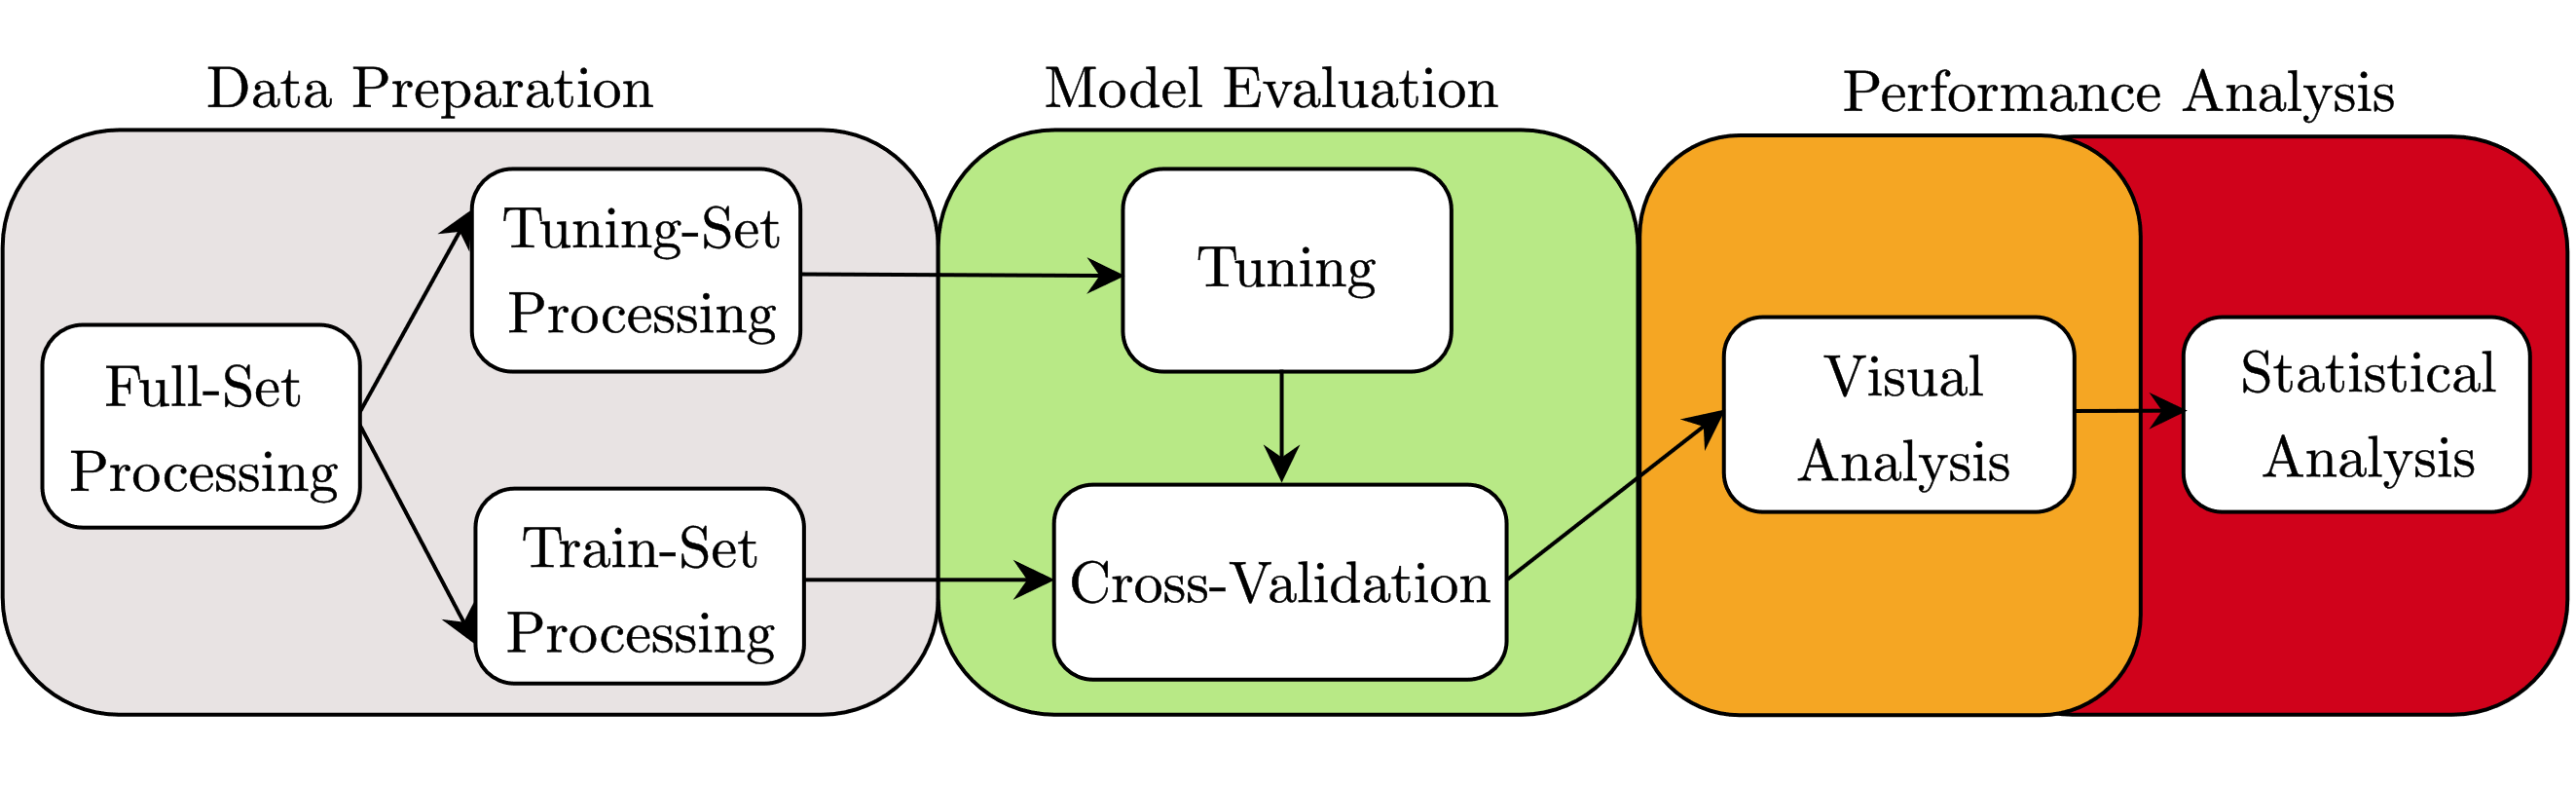
\includegraphics[width=\textwidth]{images/chapter_3/pipeline_eval.png}
    \caption[\textbf{Model implementation experimental pipeline}]{Arrows indicate the flow of the pipeline. Big coloured blocks are major pipeline steps, white rectangles indicate sub-tasks within each step.}
    \label{fig: pipeline_eval}
\end{figure}
\section{Joint Prediction of Long Term Behavioural Intensity}
\label{model_architecture_1}
In the first iteration of our model building process we focused on implementing and testing some of the core theoretical assumptions presented in chapter \ref{chapter_theory_modelling}, namely the importance of modelling temporal and non-linear dynamics in the interactions between an individual and a videogame. The experimental task used for this purpose aimed at predicting the long term intensity of interactions between an individual and a videogame given a set of behavioural metrics recorded during an initial observation period. Here, the observation period is defined as a small sequence of initial interactions between an individual and a videogame. In this specific context, we used churn and survival time as behavioural proxies for the expected intensity of future interactions. We briefly introduced these two concepts in section \ref{engagement_prediction}. More formally we can say that given a sequence of interactions with associated behavioural intensity $B_{t_1 : T}$, survival time is the amount of expected future playing activity at a given point $t_n$ \cite{ perianez2016churn, demediuk2018player, bertens2017games, kim2017churn, viljanen2018playtime}
\begin{equation}
\label{eq_survival}
    survival = \sum_{t_n}^{T}B_t
\end{equation}
while churn is the probability of observing a terminal event $C$ (usually formulated as a prolonged period of inactivity from the individual) after a given point $t_n$ \cite{hadiji2014predicting,runge2014churn, drachen2016rapid,milovsevic2017early, kim2017churn}.
\begin{equation}
\label{eq_churn}
    churn = \sum_{t_n}^{T}C_n = 1
\end{equation}
here the interactions going from $t_1: t_n$ define our observation period. It has to be noted that this task can be viewed as a special case of the more general formulation presented in section \ref{td_to_supervised}, precisely 
\begin{equation}
\label{rnn_1_exp}
   \mathbb{E}[B_{t_n : T}] = \mathbb{E}[B_{t_n : T}]
\end{equation}


and correspond to predicting extinction and future ammount of sustained engagement after observing a handful of interactions following the point of engagement (according to O'Brien et al. \cite{o2008user} framework presented in section \ref{eng_reward_motivation}). Given this experimental context, the hypotheses that we wanted to evaluate in order to support our modelling intuitions were the following:
\begin{enumerate}
    \item Leveraging all the information present in the observation period is required for achieving higher predictive power.
    \item Approaches able to account for non-linear interactions in the considered behavioural metrics can outperform simpler additive models.
    \item The ability to model the type of sequential dynamics presented in section \ref{td_to_supervised} can have a positive effect on the predictive performance.
    \item It is possible to have a single model jointly predict the considered metrics of long term behavioural intensity without any loss of predictive accuracy.
    \item It is possible to have a single model performing the predictive task simultaneously across a wide range of games.
\end{enumerate}

\subsection{Model Design}
\label{model_design_1}
The first iteration of our ANN architecture, loosely inspired by the winning entry in \cite{lee2018game}, aimed to jointly predict survival time and churn probability across a set of 6 different game contexts. This architecture, the `Bifurcating Model' (BM), is illustrated in Fig. \ref{fig: rnn_1}. 
\begin{figure}[ht]
\begin{center}
\begin{adjustbox}{width=0.7\textwidth}



\tikzset{every picture/.style={line width=0.75pt}} %set default line width to 0.75pt        

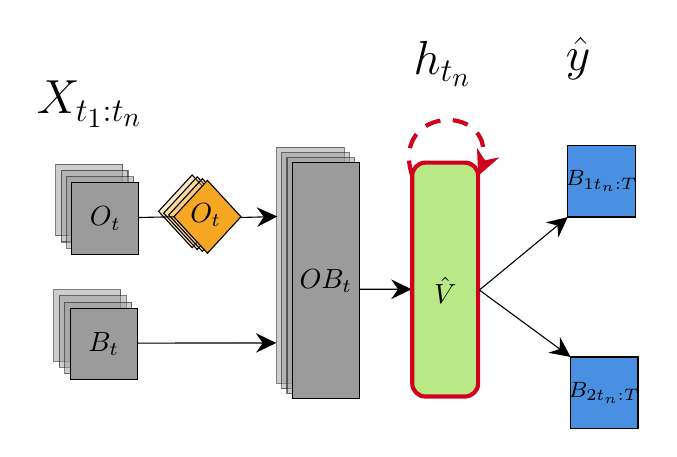
\begin{tikzpicture}[x=0.75pt,y=0.75pt,yscale=-1,xscale=1]
%uncomment if require: \path (0,300); %set diagram left start at 0, and has height of 300

%Shape: Diamond [id:dp06877884521197963] 
\draw  [fill={rgb, 255:red, 245; green, 166; blue, 35 }  ,fill opacity=0.25 ] (263.6,117.28) -- (279.77,134.81) -- (263.6,152.33) -- (247.43,134.81) -- cycle ;
%Shape: Diamond [id:dp5019197402707816] 
\draw  [fill={rgb, 255:red, 245; green, 166; blue, 35 }  ,fill opacity=0.25 ] (266.05,118.16) -- (282.22,135.68) -- (266.05,153.2) -- (249.89,135.68) -- cycle ;
%Shape: Diamond [id:dp6628494024847519] 
\draw  [fill={rgb, 255:red, 245; green, 166; blue, 35 }  ,fill opacity=0.25 ] (268.51,119.04) -- (284.68,136.56) -- (268.51,154.08) -- (252.34,136.56) -- cycle ;
%Shape: Rectangle [id:dp8304682723722553] 
\draw  [color={rgb, 255:red, 0; green, 0; blue, 0 }  ,draw opacity=0.5 ][fill={rgb, 255:red, 155; green, 155; blue, 155 }  ,fill opacity=0.5 ] (304.41,104.01) -- (336.92,104.01) -- (336.92,217.74) -- (304.41,217.74) -- cycle ;
%Shape: Rectangle [id:dp33657106031779216] 
\draw  [color={rgb, 255:red, 0; green, 0; blue, 0 }  ,draw opacity=0.5 ][fill={rgb, 255:red, 155; green, 155; blue, 155 }  ,fill opacity=0.5 ] (306.86,106.47) -- (339.38,106.47) -- (339.38,220.2) -- (306.86,220.2) -- cycle ;
%Shape: Rectangle [id:dp6698304713342962] 
\draw  [color={rgb, 255:red, 0; green, 0; blue, 0 }  ,draw opacity=0.5 ][fill={rgb, 255:red, 155; green, 155; blue, 155 }  ,fill opacity=0.5 ] (309.32,108.93) -- (341.84,108.93) -- (341.84,222.66) -- (309.32,222.66) -- cycle ;
%Shape: Diamond [id:dp7704333366065277] 
\draw  [fill={rgb, 255:red, 245; green, 166; blue, 35 }  ,fill opacity=1 ] (270.97,119.91) -- (287.13,137.43) -- (270.97,154.96) -- (254.8,137.43) -- cycle ;
%Straight Lines [id:da34159449213041837] 
\draw    (286.94,137.77) -- (301.65,137.38) ;
\draw [shift={(304.65,137.3)}, rotate = 178.49] [fill={rgb, 255:red, 0; green, 0; blue, 0 }  ][line width=0.08]  [draw opacity=0] (9.82,-4.72) -- (0,0) -- (9.82,4.72) -- (6.52,0) -- cycle    ;
%Straight Lines [id:da8208338090000002] 
\draw [fill={rgb, 255:red, 155; green, 155; blue, 155 }  ,fill opacity=1 ]   (215.09,198.3) -- (301.13,198.22) ;
\draw [shift={(304.13,198.22)}, rotate = 179.95] [fill={rgb, 255:red, 0; green, 0; blue, 0 }  ][line width=0.08]  [draw opacity=0] (9.82,-4.72) -- (0,0) -- (9.82,4.72) -- (6.52,0) -- cycle    ;
%Straight Lines [id:da7791621502079311] 
\draw [fill={rgb, 255:red, 155; green, 155; blue, 155 }  ,fill opacity=1 ]   (336.42,172.36) -- (366.33,172.35) ;
\draw [shift={(369.33,172.35)}, rotate = 179.97] [fill={rgb, 255:red, 0; green, 0; blue, 0 }  ][line width=0.08]  [draw opacity=0] (9.82,-4.72) -- (0,0) -- (9.82,4.72) -- (6.52,0) -- cycle    ;
%Shape: Rectangle [id:dp3847312278870677] 
\draw  [color={rgb, 255:red, 0; green, 0; blue, 0 }  ,draw opacity=0.5 ][fill={rgb, 255:red, 155; green, 155; blue, 155 }  ,fill opacity=0.5 ] (197.01,172.53) -- (229.26,172.53) -- (229.26,207.05) -- (197.01,207.05) -- cycle ;
%Shape: Rectangle [id:dp5169374919332619] 
\draw  [color={rgb, 255:red, 0; green, 0; blue, 0 }  ,draw opacity=0.5 ][fill={rgb, 255:red, 155; green, 155; blue, 155 }  ,fill opacity=0.5 ] (199.63,175.51) -- (231.88,175.51) -- (231.88,210.03) -- (199.63,210.03) -- cycle ;
%Shape: Rectangle [id:dp7025889851900418] 
\draw  [color={rgb, 255:red, 0; green, 0; blue, 0 }  ,draw opacity=0.5 ][fill={rgb, 255:red, 155; green, 155; blue, 155 }  ,fill opacity=0.5 ] (202.27,178.56) -- (234.53,178.56) -- (234.53,213.08) -- (202.27,213.08) -- cycle ;
%Shape: Rectangle [id:dp34989838660273853] 
\draw  [fill={rgb, 255:red, 155; green, 155; blue, 155 }  ,fill opacity=1 ] (204.86,181.5) -- (237.11,181.5) -- (237.11,216.02) -- (204.86,216.02) -- cycle ;
%Shape: Rectangle [id:dp10413248734443492] 
\draw  [fill={rgb, 255:red, 155; green, 155; blue, 155 }  ,fill opacity=1 ] (311.77,111.39) -- (344.29,111.39) -- (344.29,225.12) -- (311.77,225.12) -- cycle ;
%Shape: Rectangle [id:dp5251277777045114] 
\draw  [color={rgb, 255:red, 0; green, 0; blue, 0 }  ,draw opacity=0.5 ][fill={rgb, 255:red, 155; green, 155; blue, 155 }  ,fill opacity=0.5 ] (197.83,112.08) -- (230.08,112.08) -- (230.08,146.6) -- (197.83,146.6) -- cycle ;
%Shape: Rectangle [id:dp04395321919357453] 
\draw  [color={rgb, 255:red, 0; green, 0; blue, 0 }  ,draw opacity=0.5 ][fill={rgb, 255:red, 155; green, 155; blue, 155 }  ,fill opacity=0.5 ] (200.45,115.06) -- (232.7,115.06) -- (232.7,149.58) -- (200.45,149.58) -- cycle ;
%Shape: Rectangle [id:dp5987068943888822] 
\draw  [color={rgb, 255:red, 0; green, 0; blue, 0 }  ,draw opacity=0.5 ][fill={rgb, 255:red, 155; green, 155; blue, 155 }  ,fill opacity=0.5 ] (203.09,118.11) -- (235.35,118.11) -- (235.35,152.63) -- (203.09,152.63) -- cycle ;
%Shape: Rectangle [id:dp34752966033388544] 
\draw  [fill={rgb, 255:red, 155; green, 155; blue, 155 }  ,fill opacity=1 ] (205.68,121.05) -- (237.93,121.05) -- (237.93,155.57) -- (205.68,155.57) -- cycle ;
%Straight Lines [id:da167964927096784] 
\draw    (237.82,137.77) -- (254.8,137.43) ;
%Rounded Rect [id:dp23035038317630208] 
\draw  [color={rgb, 255:red, 208; green, 2; blue, 27 }  ,draw opacity=1 ][fill={rgb, 255:red, 184; green, 233; blue, 134 }  ,fill opacity=1 ][line width=1.5]  (369.64,117.69) .. controls (369.64,114.18) and (372.48,111.34) .. (375.99,111.34) -- (395.05,111.34) .. controls (398.56,111.34) and (401.4,114.18) .. (401.4,117.69) -- (401.4,217.68) .. controls (401.4,221.19) and (398.56,224.03) .. (395.05,224.03) -- (375.99,224.03) .. controls (372.48,224.03) and (369.64,221.19) .. (369.64,217.68) -- cycle ;
%Curve Lines [id:da1309582955199332] 
\draw [color={rgb, 255:red, 208; green, 2; blue, 27 }  ,draw opacity=1 ][line width=1.5]  [dash pattern={on 5.63pt off 4.5pt}]  (369.64,117.69) .. controls (358.28,83.07) and (412.82,81.85) .. (402.76,114.05) ;
\draw [shift={(401.4,117.69)}, rotate = 293.32] [fill={rgb, 255:red, 208; green, 2; blue, 27 }  ,fill opacity=1 ][line width=0.08]  [draw opacity=0] (12.23,-5.88) -- (0,0) -- (12.23,5.88) -- (8.12,0) -- cycle    ;
%Shape: Rectangle [id:dp505523013710797] 
\draw  [fill={rgb, 255:red, 74; green, 144; blue, 226 }  ,fill opacity=1 ] (444.61,103.03) -- (477.11,103.03) -- (477.11,137.53) -- (444.61,137.53) -- cycle ;
%Shape: Rectangle [id:dp241922601816576] 
\draw  [fill={rgb, 255:red, 74; green, 144; blue, 226 }  ,fill opacity=1 ] (445.94,204.96) -- (478.44,204.96) -- (478.44,239.46) -- (445.94,239.46) -- cycle ;
%Straight Lines [id:da6479510532261308] 
\draw    (402,172.73) -- (442.3,139.44) ;
\draw [shift={(444.61,137.53)}, rotate = 140.44] [fill={rgb, 255:red, 0; green, 0; blue, 0 }  ][line width=0.08]  [draw opacity=0] (9.82,-4.72) -- (0,0) -- (9.82,4.72) -- (6.52,0) -- cycle    ;
%Straight Lines [id:da5488291959914686] 
\draw    (402,172.73) -- (443.52,203.18) ;
\draw [shift={(445.94,204.96)}, rotate = 216.26] [fill={rgb, 255:red, 0; green, 0; blue, 0 }  ][line width=0.08]  [draw opacity=0] (9.82,-4.72) -- (0,0) -- (9.82,4.72) -- (6.52,0) -- cycle    ;

% Text Node
\draw (220.99,198.76) node  [font=\normalsize]  {$B_{t}$};
% Text Node
\draw (385.52,172.8) node  [font=\normalsize]  {$\hat{V}$};
% Text Node
\draw (270.15,136.56) node  [font=\normalsize]  {$O_{t}$};
% Text Node
\draw (214.34,83.25) node  [font=\LARGE]  {$X_{t_{1} :t_{n}}$};
% Text Node
\draw (328.03,168.25) node  [font=\normalsize]  {$OB_{t}$};
% Text Node
\draw (221.81,138.31) node  [font=\normalsize]  {$O_{t}$};
% Text Node
\draw (384.34,63.6) node  [font=\LARGE]  {$h_{t_{n}}$};
% Text Node
\draw (460.86,120.28) node  [font=\footnotesize]  {$B_{1t_n:T}$};
% Text Node
\draw (462.19,222.21) node  [font=\footnotesize]  {$B_{2t_n:T}$};
% Text Node
\draw (449.54,61) node  [font=\LARGE]  {$\hat{y}$};

\end{tikzpicture}

\end{adjustbox}
\end{center}
\caption[\textbf{The bifurcating model (BM) architecture}]{Blue, orange and green shapes represent respectively feedforward, embedding and LSTM operations. Gray shapes indicate operations with no learnable parameters, such as tensor instantiation and concatenation. Stacked, transparent colouring indicates tensors with a sequential structure. Straight and curved arrows refer to the presence of feed-forward or recurrent information flow. The red highlight shows the portion of the model we hypothesize is inferring an approximation of attributed incentive salience.}
\label{fig: rnn_1}
\end{figure}
The model receives as input a set of variable length multivariate time series composed of 5 metrics described in section \ref{data_1}, resulting in an $B \in \mathbb{R}^{N \times T \times 5}$ tensor where $N$ is the number of time series and $T$ is the length of the longest series. All the series shorter then $T$ are made of the same length by adding a padding value $pad=9999$ at the end (this value will never appear in the dataset). An additional set of univariate time series of shape $O \in \mathbb{N}^{N \times 1 \times 1}$ is used for indicating to which game context the behavioural metrics belongs to.  It has to be noted that these series contain numerical encoding of the game context (e.g. $jc3 \mapsto 1$, $lis \mapsto 2$ etc.) in order to be able to represent the associated information through a so called embedding operation (see Appendix \ref{embedding_operation}). Given the input series, the operation will generate an $O^* \in \mathbb{R}^{N \times T \times h}$  tensor with $h$ being the number of hidden units chosen for the embedding. This can be thought as a form of over-parametrization that allows each single context to have a non-sparse representation and to be projected into a multi-dimensional space where the relationships between elements become meaningful (e.g. game contexts which are similar to each other in respect to the objectives will be located closer to each other in the embedding space). This, other than allowing each context to carry more information, provides a general representation that grows richer and richer the more categories are included into it. Obviously this would require to re-fit the model whenever a new unseen context is added as this approach does not support out-of-sample generalizability. It is important to highlight that this embedding operation is fundamental to the construction of a global model as outlined in section \ref{manifold_learning}. Indeed, it allows to appropriately associate parameters to all the game contexts taken in consideration and to include them in a single model. Next, the raw behavioural input and the embedded game context vector are concatenated along the temporal dimension producing a single $OB \in \mathbb{R}^{N \times T \times h + 5}$ tensor and a masking operation is applied. This operation allows the model to skip computations whenever the $pad$ value is encountered \cite{chollet2015keras}. These newly obtained features are then modelled across time using a recurrent neural network (RNN) with Long Short-Term Memory (LSTM) operations (see Appendix \ref{lstm_operation}). In this specific setting the RNN is of type many-to-one \cite{bengio2017deep} therefore producing an $H \in \mathbb{R}^{N \times h}$ matrix (with $h$ being the number of hidden units chosen for the recurrent operation). As we already highlighted in section \ref{td_to_supervised} the use of an RNN in this context is of pivotal importance for modelling the sequential dynamics underlying the process of incentive salience attribution. Indeed, if we think of the representation generated by the RNN in terms of expectation
\begin{equation}
\label{rnn_1_exp}
   \mathbb{E}[B_{t_n : T}] = f(h_{t_n}; \theta)
\end{equation}
what the LSTM operation allows us to do is to estimate $h_{t_n}$ as the result of a process with memory where the intensity of previous interactions with a specific game determines the expected intensity of all future interactions. The final step of this architecture uses the latent representation generated by the RNN for producing predictions for survival time and churn. This is accomplished by means of multi-task learning with two ANNs with fully connected operation (see Appendix \ref{fnn_operation}) receiving the matrix generated by the RNN as input and producing the predictions for the relative behavioural targets in the form of a vector of shape $\hat{y} \in \mathbb{R}^{N}$. The model used $ReLU$ as activation function (see Appendix \ref{relu}) for the hidden units whereas the link functions used for generating churn and survival time predictions were the $identity$ (see Appendix \ref{identity}) and $sigmoid$ (see Appendix \ref{sigmoid}) functions. We applied two regularization techniques after each fully connected operation, namely: batch normalization \cite{ioffe2015batch} and dropout \cite{srivastava2014dropout} (see Appendix \ref{dropout} and \ref{batch_norm}).

\paragraph*{Competing Models}
\label{competing_models_1}
In order to test the hypotheses mentioned in section \ref{model_architecture_1} we implemented a series of competing models for disjoint estimation of survival time and churn probability. Furthermore, we decided to include a baseline model (MM) which generates predictions based on the average of the targets in the training set. The presence of a baseline which doesn't require any form of parameters estimation provides a sanity check on the overall quality of the models and complexity of the problem at hands (e.g. if a  predictive task is trivial to solve we expect a relatively satisfactory level of accuracy even by a naive baseline model). The competing models were chosen according to two main criteria: the ability to capture linear and non-linear interactions between features and most importantly the capability to fit large data-sets (e.g. matrix of dimension $x \in \mathbb{R}^{\approx10^6\times10^2}$). According to this criteria we opted for linear regression with ElasticNet regularization (see appendix \ref{enet_reg}) (EN) \cite{zou2005regularization}, logistic regression (LR) and two Multi-Layer Perceptrons using  $id$ (MLPr) and $sigma$ (MLPc) as link functions. Multi-Layer Perceptrons are ANNs using the type of feedforward operation described in Appendix \ref{fnn_operation}. We felt that given the similarities between linear models and ANNs, which can be seen as a stacked version of the former but with more `expressive power', the chosen algorithms constituted a natural progression in the modelling approach. 

\subsection{Data}
\label{data_1}
In order to evaluate the performance of the different models in the experimental predictive task, we needed to acquire records of interactions between individuals and potentially rewarding objects in naturalistic contexts. As mentioned in section \ref{videogame_telemetries}, video games are particularly suited for this purpose given their learning-dependent reinforcing properties and the large amount of longitudinal data streams that they can generate. For this reason we gathered data from six different games published by our partner company, \textit{Square Enix Ltd}. Focusing on maintaining heterogeneity in genre and platform, we considered the following titles: \emph{Hitman Go} (hmg), \emph{Hitman Sniper} (hms), \emph{Just Cause 3} (jc3), \emph{Just Cause 4} (jc4), \emph{Life is Strange} (lis), and \emph{Life is Strange: Before the Storm} (lisbf). A general description of each of these titles can be found in Table \ref{game_description_31}. Due to the diversity in their in-game mechanics, each of these games was considered as an "object" with different reinforcing properties (see section \ref{videogame_telemetries}). This allowed us to mimic a situation where a single model had access to data coming from a heterogeneous set of potentially rewarding entities (similarly to what we described in section \ref{motivation_hist}). Data were gathered from any user playing between the game's release and February 2019, allowing us to adopt more robust sampling strategies which for each game utilizes the breadth of virtually the entire user-base. To rule out possible `faulty' but not `naturally abnormal' data, we restricted the data cleaning process to a single filter applied at query time to ignore users having at least one of the considered metric over the game population's \nth{99} percentile. This allowed us to make little assumptions on the distribution of the data as well as providing a convenient stress test for eventual future applications.

\begin{table}[h] 
\centering
\caption{\textbf{Data-set Description}. For each game we retrieved 80,000 Churners and 80,000 Non-Churners randomly sampled from all the available users.}
\label{gamesdescription}
\begin{tabularx}{\textwidth}{@{}lrrrrrrX@{}}
\toprule

\multirow{2}{*}{\textbf{Game}} & \multicolumn{2}{l}{\textbf{Survival Time (Mins})} & \multirow{2}{*}{\textbf{Churners}} & \multirow{2}{*}{\textbf{Non Churners}} & \multicolumn{2}{l}{\textbf{Observation Period}} & \multirow{2}{*}{\textbf{Type}} \\ \cmidrule(lr){2-3} \cmidrule(lr){6-7}
                      & \textbf{Min}                  & \textbf{Max}                  &                           &                               & \textbf{Min}                & \textbf{Max}               &                                \\ \midrule
hmg                        & 11 & 260    & 80,000 & 80,000  & 1  & 7  & Mobile Strategy                       \\
hms                        & 2 & 454     & 80,000 & 80,000  & 1  & 15 & Mobile Shooting Gallery                \\
jc3                        & 32 & 12,695 & 80,000 & 80,000  & 1  & 20 & Console Action Open World             \\
jc4                        & 7 & 1,135   & 80,000 & 80,000  & 1  & 9  & Console Action Open World           \\
lis                        & 5 & 704     & 80,000 & 80,000  & 1  & 6  & Console Graphic Adventure \\
libf                       & 14 & 1,214  & 80,000 & 80,000  & 1  & 10 &  Console Graphic Adventure \\ \bottomrule
\end{tabularx}
\end{table}

\paragraph*{Defining the Observation Period}
Because we were interested in predicting survival time and churn probability based only on a restricted number of early individual-game interactions it was important to define a cut-off for what would be considered an "early sequence of interactions" (the so called observation period (OP)). Choosing the length for the OP was not a trivial task as there is little indication in the literature about optimal cut-off values. Hence, we decided to visually inspect the data a-priori and extend rules proposed in \cite{drachen2016rapid, milovsevic2017early} to take into account natural inter-individual differences. Therefore, we defined the cut-off as:

\begin{equation}
\label{cutoffop}
    \text{cutoff} = 
    \Biggl\lceil
        \dfrac
            {min(T, completion_t)}
            {3}
    \Biggr\rceil
\end{equation}

Where $T$ is the total number of game play sessions and $completion_t$ is the number of game play sessions before the user completed the game for the first time. In this way we take the first $\frac{1}{3}$ of all played sessions for players who churned and the first $\frac{1}{3}$ of played sessions before a non-churning player completed the game for the first time. We apply this cut off to the ordered list of all recorded play sessions for a specific user. We decided to use game sessions as the temporal dimension, rather than total minutes played, since we believed it better adjusted for each user's "pace" (i.e. not all the users have the possibility to play at the same frequency). Since the length of the OP has a naturally different distribution between the churning and non-churning population, we stratified our sampling technique to maintain a similar ratio of OP lengths among churners and non churners. This becomes particularly relevant when employing models that leverage the entire sequence of interactions where the length of the OP could leak information about the considered targets (e.g. churn is on average associated with a small number of interactions). Summarizing, if an individual had 9 total sessions recorded, we considered the first 3 for making predictions on what happened from the $4^{th}$ to the $9^{th}$ session. 

\paragraph*{Defining the Behavioural Metrics and Targets}
\label{behavioural_metric_targets_1}
We considered a set of 5 metrics, easily generalizable across games and comparable with metrics employed in other behavioural studies of incentive salience attribution \cite{berridge1998role,mcclure2003computational,zhang2009neural}, and retrieved them temporally  (i.e. over each game session during the OP), see Table \ref{metricsdescription_1} for a description. Additionally, we acquired a single context feature specifying the game context from where the metrics were originated. For determining the targets for our survival and churn estimation tasks, we leveraged existing literature on churn prediction \cite{drachen2016rapid, milovsevic2017early, lee2018game, perianez2016churn, runge2014churn, kim2017churn, hadiji2014predicting, xie2015predicting} and survival analysis \cite{viljanen2018playtime, demediuk2018player, lee2018game, bertens2017games}, extending existing rules to accommodate the need to define churn and survival time in single player games with a defined life cycle (i.e. non Games-as-a-Service GaaS). Indeed, while GaaS can only rely on inactivity periods for determining churn, titles with a defined life cycle (e.g. single player games) can utilize a defined end-game period as a hard cut-off for distinguishing between churners and non-churners: users finishing a game are not churners even if they stop playing afterwards. In this view, we took advantage of having access to the complete session history for all users to create a churn definition which was robust to the variance in play patterns across games by taking into account all the recorded inter-session distances. The criteria we adopted for defining a user as churner were both: 

\begin{enumerate}
    \item Not completing the game
    \item Being inactive for a period equal or greater to:
        \begin{equation}
            \label{inactivityrule}
            \text{inactivity} = 
            mean(\mathbf{x}) + 2.5 \cdot std(\mathbf{x})
        \end{equation}
\end{enumerate}

For better adjusting for inter-individual differences, we could have applied formula \ref{inactivityrule} to each user individually but this could have created accuracy issue for individuals with very few recorded sessions. Therefore, we opted for a conservative but more robust approach applying inactivity ($\mathbf{x}$) $\forall \mathbf{x} \in X$ where $X$ is the collection of all the considered games and $\mathbf{x}$ is the vector of inter-sessions distances in minutes for a specific game. The use of formula \ref{inactivityrule} allowed us to estimate an inactivity period which was not arbitrarily chosen but statistically defined as "extraordinary long" in accordance with characteristics of play patterns in a particular game. For defining the survival time, we simply computed the total amount of play time in minutes for a user minus the amount of play time during the OP.

\begin{table}[H] \centering
\caption[Description of Selected Telemetries]{Description of selected telemeteries}
\label{metricsdescription_1}
  \begin{tabularx}{\textwidth}{@{}lX@{}}
    \toprule
    \textbf{Metric}      & \textbf{Description}          \\ \midrule
    {Absence}    & Temporal distance between sessions (hours)  \\
    {Session Time}     & Overall session duration (minutes)       \\ 
    {Session Activity}    & Count of user initiated gameplay-related actions. E.g. "Attack an enemy" is considered a valid action while "Being attacked by an enemy" is not.\\
    {Session Diversity}      & Number of distinct gameplay-related actions  \\ 
    {N°Sessions}    & Number of played sessions.\\ 
    {Context}    &  Game context identifier.  \\
    \bottomrule
  \end{tabularx}
\end{table}

\paragraph*{Data Preparation}
\label{data_preparation_1}
We adopted specific data preparation for testing the various hypotheses specified in section \ref{model_architecture_1}. We first generated a dataset collapsing the original data over the temporal dimension retrieving mean and standard deviation of each considered metric and adding a one-hot encoded (see Appendix \ref{one_hot_encode_operation} version of the game context indicator. Then we generated a second data-frame maintaining the original temporal structure and numerically encoding the game context indicators. As we mentioned before, different users had OP of different lengths so we applied the $pad$ value to each metric column in the data-set so to have each sequence of considered sessions to the length of the longest sequence in the data-set. For each experiment we created a tuning and test subsets (i.e. 20 and 80 \% of the original data-set) via stratified shuffle split \cite{scikit-learn}, employing the first for hyper-parameters tuning and the second for model evaluation. Each time a model was fit on the considered dataset, we re-scaled each metric separately for each game in an outliers-robust way:
\begin{equation}
\label{robustscaler}
    \text{RobustRescale}=
        \dfrac
            {\mathbf{x} - Q_2(\mathbf{x})}
            {Q_3(\mathbf{x}) - Q_1(\mathbf{x})}
\end{equation}
where $\mathbf{x}$ is the feature vector to be re-scaled and $Q_n$ is the $n^{th}$ quartile. 

\subsection{Model Tuning and Comparison}
\label{tuning_comparison_1}
For all the considered models we first, determined the best hyper-parameters via simple grid search 10-fold stratified cross validation \cite{scikit-learn} on the tuning set. At each iteration of the 10-fold stratified cross validation a small sub-set of the fold used for fitting the model (i.e. 10\%) was set aside and used to evaluate model convergence and eventually trigger an early-stopping policy (so to avoid over-fitting). For all the models convergence was determined by the loss not improving for at least 3 consecutive epochs. The models were trained though mini-batch stochastic gradient descent (using a batch size of 256) using the Adaptive Moment Estimation (ADAM) optimizer \cite{kingma2014adam} with learning rate adjusted through a cyclical policy \cite{smith2017cyclical, chollet2015keras}. We used Mean Squared Error (MSE) and Binary Cross Entropy (BCE) respectively (see Appendix \ref{mse} and \ref{bce}) as objective functions for the disjoint models (i.e. linear models and MLPs). Differently from the other models the objective function for the the BM model was given by the unweighted sum of the losses associated with the two branching ANNs, namely BCE for the churn prediction task and the Symmetric Mean Absolute Percentage Error (SMAPE) (see Appendix \ref{smape}) for the survival prediction task. The SMAPE is bounded between 0 and 100 and can be interpreted as percentage deviation from the target with lower values indicating better model fit. The choice of SMAPE was motivated by the fact that its scale invariance allowed better comparisons of results across game contexts. For EN the best hyper-parameters were $\lambda = 0.1$ and $alpha=0.5$ for the regularization term regularization. For LR a $\lambda = 0.01$ for the lasso regularization was found to yield the best results. Both MLPr and MLPc employed an Ridge regularization with $\lambda=0.01$ and utilized a 3 layers architecture with 200, 100 and 50 hidden units. The BM architecture used an embedding with 40 hidden units, an LSTM RNN with 100 hidden units and two fully connected ANNs with 300 hidden units each. The best dropout rate was found to be $p=0.1$ meaning that at each forward pass 1 in ten units for the fully connected ANNs were set to 0. Once the best hyper-parameters were found, each model was evaluated on the the test by fitting it on 90\% of the set and performing out-of-sample prediction for the remaining 10\%. All the disjoint models were tested on both the collapsed and unfolded datasets while the BM model only on the last one. This is because the BM model was specifically designed for performing predictions using data in a time series format. Moreover, following the intuition from \cite{gal2016dropout}, the BM model supported Montecarlo dropout: a method for approximating Bayesian inference and producing posterior distribution of the model's predictions. This was achieved by querying the model 50 times at prediction time and retaining all the produced values. When computing the performance metrics we then used the mean of the estimated values, since they roughly followed a normal distribution. For the churn prediction task the chosen metric was the macro-averaged F1 score (see Appendix \ref{F1}) (i.e. employing the unweighted mean of precision and recall for both classes) while for the survival time prediction task the chosen metric was the SMAPE. The code for tuning and evaluating the models was written in Python 3.6, with the algorithms provided by the library scikit-learn \cite{scikit-learn} and  Keras (with Tensorflow as a back-end) \cite{chollet2015keras}.

\subsection{Results}
\label{results_1}
We will first present results for each disjoint model as well as for the baseline model. Next we will illustrate in detail the performance of the BM model both in terms of its raw accuracy and its capability to include uncertainty in its predictions. Note that for all reported SMAPE results the smaller the better as it represents the error between the prediction and ground truth. Conversely, for F1 the larger the better since it measures the discriminate power of the models on a classification task. The probability threshold employed for discriminating between classes was set to $p=0.5$. We want to highlight that, given our chosen model evaluation strategy, all the results presented here report the expected value (i.e. the mean) of a scoring metric over a single hold-out test hence conventional sample-based statistical analysis are not feasible. However, in order to quantify the uncertainty in the computed evaluation metrics we reported the standard error of the mean along with the expected value. For example in the case of SMAPE we can see from the formula in Appendix \ref{smape} that the metric computes the empirical mean over the Symmetric Percentage Error (SAPE), in order to obtain a measure of uncertainty of this estimate is sufficient to compute $SE_{SAPE} = \frac{\sigma_{SAPE}}{N}$ with $\sigma_{SAPE}$ being the standard deviation of the SAPE computed over the entire test set $N$. Moreover in order to gather a general sense of global performance, in Figure \ref{model_comp_coll_31} for each model we visualized the expected performance collapsing on game context.
\begin{figure*}[h]
\centering
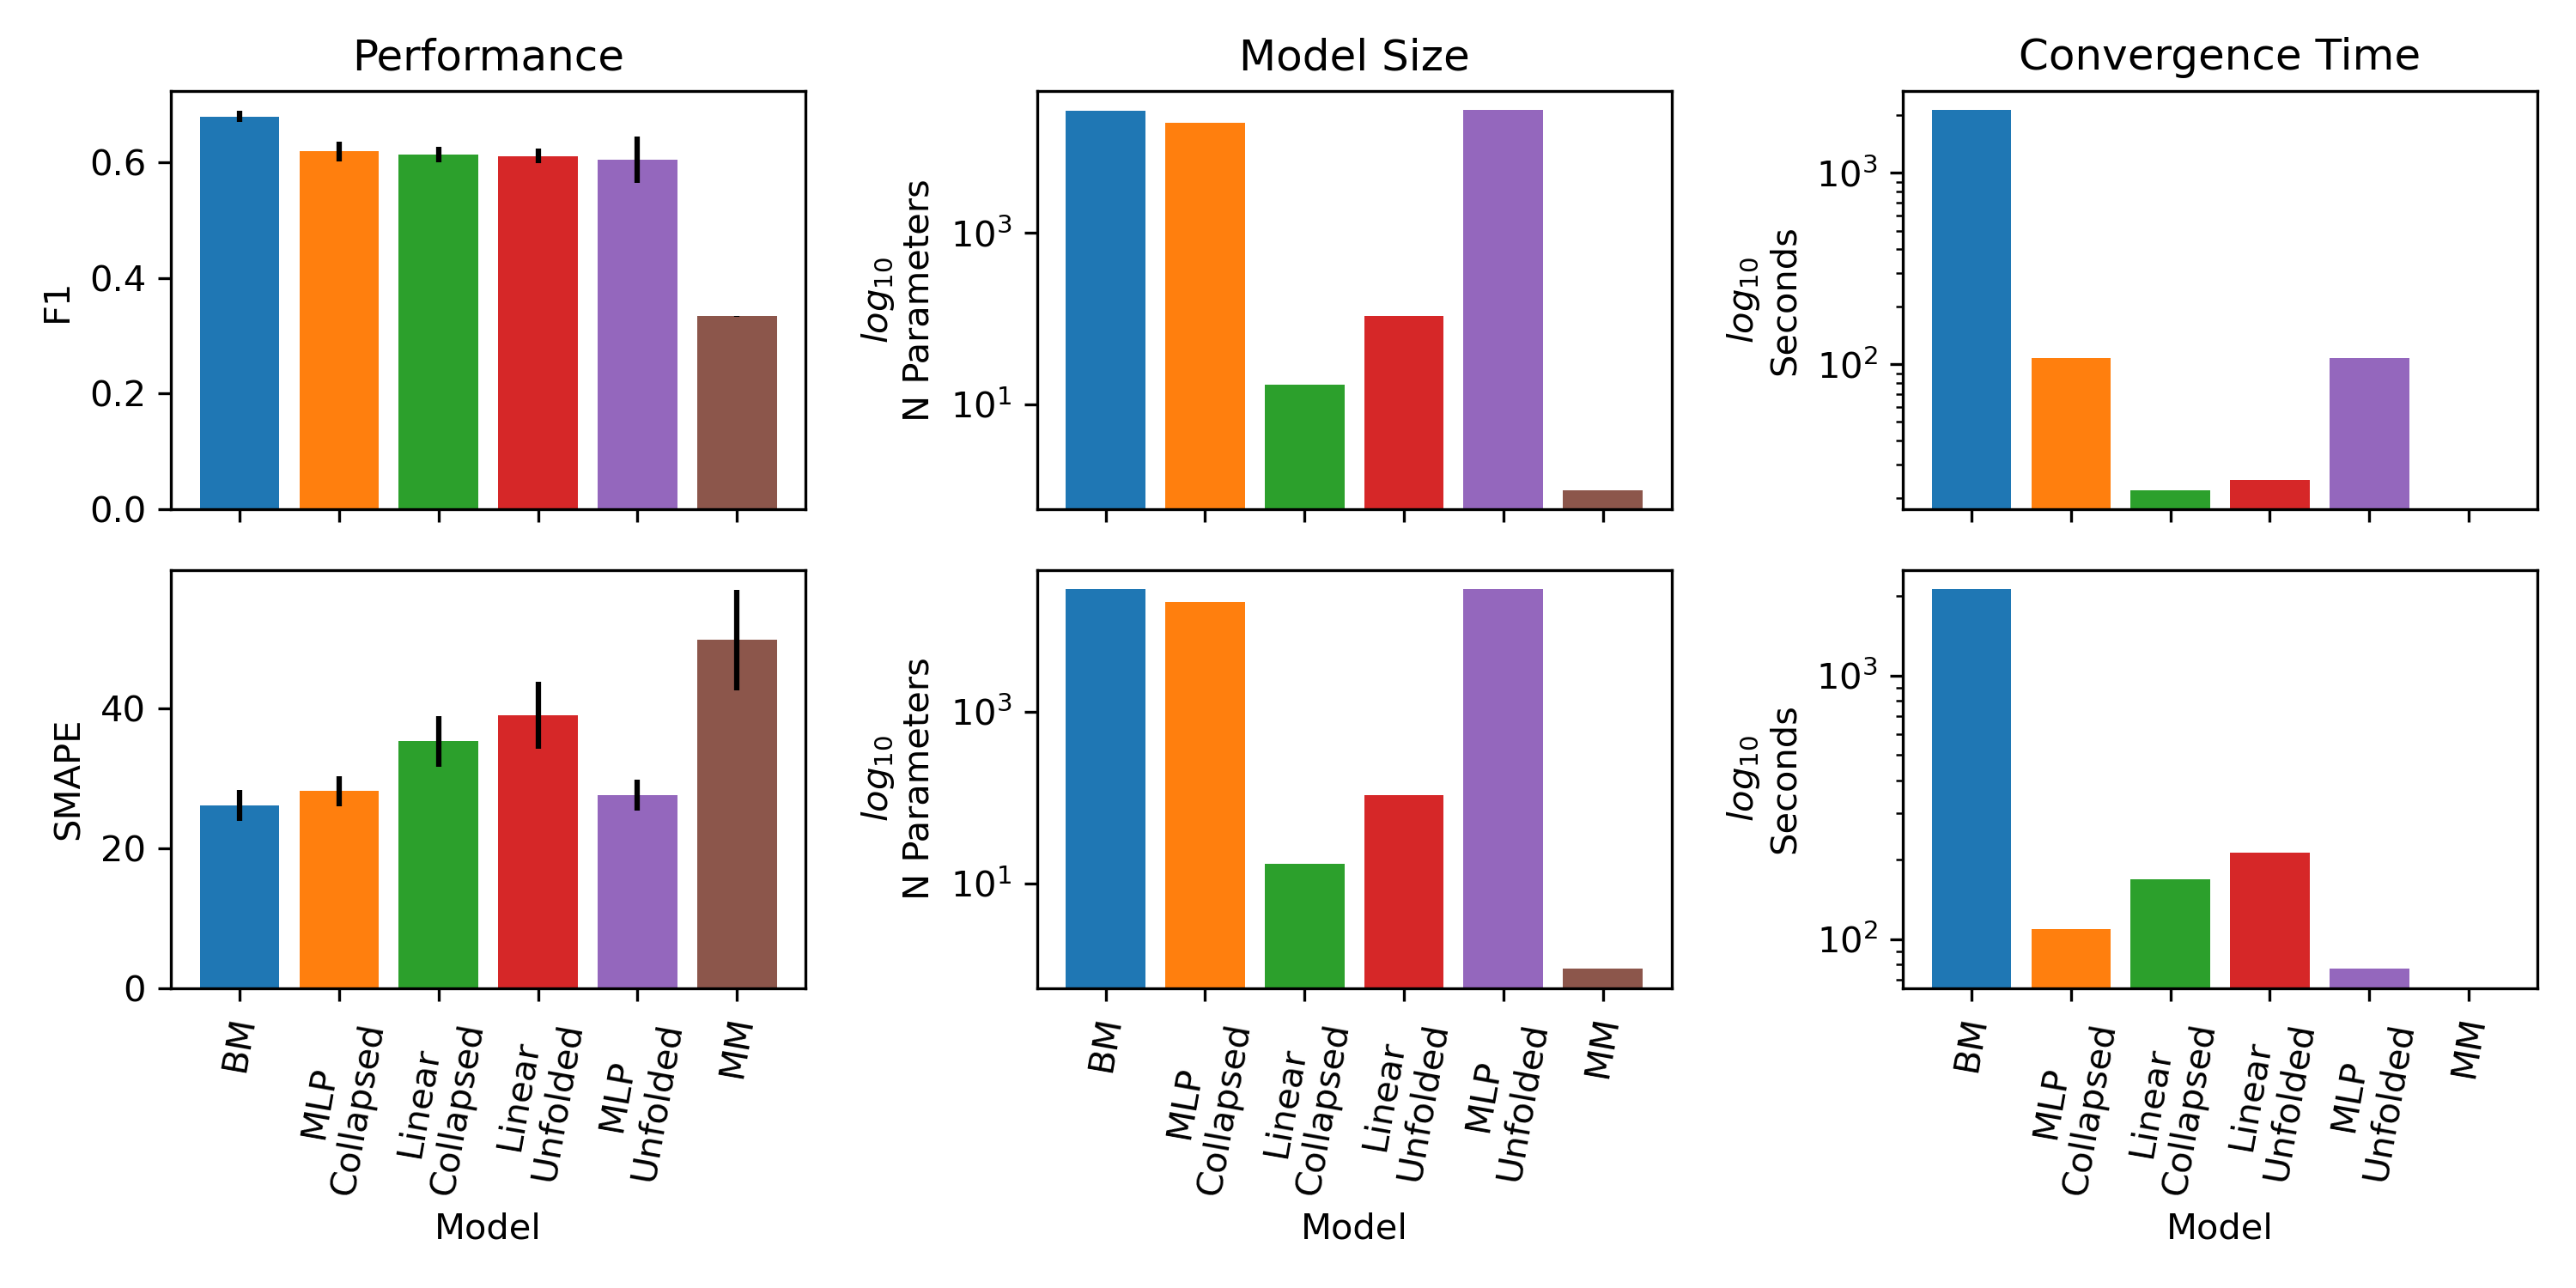
\includegraphics[width=.8\textwidth]{images/chapter_3/global_31.png}
\caption[\textbf{Aggregated comparison of models' performance}]{The BM architecture outperformed all competing ones on both target using however more parameters and computation time. Bar-plots in the first column show the average performance across the 6 game contexts along with estimated standard errors of the mean. The bar-plots on the second and third columns express the number of parameters and the convergence time for each model.}
\label{model_comp_coll_31} 
\end{figure*}
\begin{table}[h]\centering
\caption{\textbf{Performance Baseline Mean Model}}
\label{baseperformance}
\resizebox{0.5\textwidth}{!}{
\begin{tabular}{@{}llrr@{}}
\toprule
\textbf{Game}  &\textbf{Model}                 & \textbf{SMAPE}      & \textbf{F1}       \\ \midrule
\textbf{hmg}   &\multirow{2}{*}{}               & $0.767 \pm 0.001$   & $0.500 \pm 0.003$ \\
\textbf{hms}   &                                & $0.581 \pm 0.001$   & $0.507 \pm 0.003$ \\
\textbf{jc3}   &\multirow{2}{*}{\textbf{MM}}    & $0.632 \pm 0.003$   & $0.499 \pm 0.004$ \\
\textbf{jc4}   &                                & $0.366 \pm 0.002$   & $0.499 \pm 0.001$ \\
\textbf{lis}   &\multirow{2}{*}{\textit{}}      & $0.404 \pm 0.001$   & $0.500 \pm 0.003$ \\
\textbf{lisbf} &                                & $0.244 \pm 0.002$   & $0.500 \pm 0.005$ \\ \bottomrule
\end{tabular}
}
\end{table}
The results from the predictive task carried out using the collapsed dataset, Table \ref{collapsedperformance}, showed how all the 4 models strongly outperformed the MM baseline, Table \ref{baseperformance}, in all games, while also achieving an overall satisfying performance. Moreover we noticed how MLPr and MLPc markedly outperformed EN and LR in both churn probability and survival time prediction across all games.  
\begin{table}[h] \centering
\caption{\textbf{Performance Collapsed Format}}
\label{collapsedperformance}
\resizebox{0.5\textwidth}{!}{
\begin{tabular}{@{}llrlr@{}}
\toprule
\textbf{Game}  &\textbf{Model}                & \textbf{SMAPE}       &\textbf{Model}                & \textbf{F1}       \\ \midrule
\textbf{hmg}   &\multirow{2}{*}{}             & $51.3 \pm 4.3$    &\multirow{2}{*}{}             & $0.591 \pm 0.004$ \\
\textbf{hms}   &                              & $33.1 \pm 2.0$    &                              & $0.624 \pm 0.004$ \\
\textbf{jc3}   &\multirow{2}{*}{\textbf{EN}}  & $42.3 \pm 0.8$    &\multirow{2}{*}{\textbf{LR}}  & $0.601 \pm 0.004$ \\
\textbf{jc4}   &                              & $35.1 \pm 0.6$    &                              & $0.663 \pm 0.002$ \\
\textbf{lis}   &\multirow{2}{*}{}             & $28.7 \pm 0.4$    &\multirow{2}{*}{}             & $0.626 \pm 0.003$ \\
\textbf{lisbf} &                              & $23.9 \pm 0.3$    &                              & $0.591 \pm 0.003$ \\ \midrule

\textbf{hmg}   &\multirow{2}{*}{}             & $30.4 \pm 0.8$    &\multirow{2}{*}{}             & $0.660 \pm 0.006$ \\
\textbf{hms}   &                              & $24.1 \pm 0.7$    &                              & $0.670 \pm 0.006$ \\
\textbf{jc3}   &\multirow{2}{*}{\textbf{MLPr}}& $36.0 \pm 0.3$    &\multirow{2}{*}{\textbf{MLPc}}& $0.654 \pm 0.004$ \\
\textbf{jc4}   &                              & $33.4 \pm 0.2$    &                              & $0.678 \pm 0.004$ \\
\textbf{lis}   &\multirow{2}{*}{\textit{}}    & $25.6 \pm 0.3$    &\multirow{2}{*}{\textit{}}    & $0.664 \pm 0.003$ \\
\textbf{lisbf} &                              & $21.9 \pm 0.2$    &                              & $0.622 \pm 0.003$ \\ \bottomrule
\end{tabular}
}
\end{table}
Looking at the same modelling approaches on the unfolded version of the same dataset we can observed a similar pattern of results, see Table \ref{unfoldedperformance}, regarding baseline and inter-models comparisons. However, it was clear that using unfolded, temporal data lead to only small improvements over the aggregated data. This might be explained by the fact that the chosen modelling approaches are not explicitly designed for taking temporal structure into account, for example they have no explicit mechanics for temporal modelling such as those provided by a LSTM.
\begin{table}[h] \centering
\caption{\textbf{Performance Unfolded Format}}
\label{unfoldedperformance}
\resizebox{0.5\textwidth}{!}{
\begin{tabular}{@{}llrlr@{}}
\toprule
\textbf{Game}  &\textbf{Model}                 & \textbf{SMAPE}  &\textbf{Model}               & \textbf{F1}       \\ \midrule
\textbf{hmg}   &\multirow{2}{*}{}             & $54.5 \pm 2.4$ &\multirow{2}{*}{}             & $0.612 \pm 0.004$ \\
\textbf{hms}   &                              & $55.0 \pm 2.0$ &                              & $0.626 \pm 0.004$ \\
\textbf{jc3}   &\multirow{2}{*}{\textbf{EN}}  & $38.4 \pm 0.3$ &\multirow{2}{*}{\textbf{LR}}  & $0.607 \pm 0.003$ \\
\textbf{jc4}   &                              & $34.9 \pm 0.2$ &                              & $0.660 \pm 0.003$ \\
\textbf{lis}   &\multirow{2}{*}{}             & $30.2 \pm 0.1$ &\multirow{2}{*}{}             & $0.641 \pm 0.004$ \\
\textbf{lisbf} &                              & $23.5 \pm 0.2$ &                              & $0.578 \pm 0.003$ \\ \midrule
\textbf{hmg}   &\multirow{2}{*}{}             & $29.3 \pm 0.4$ &\multirow{2}{*}{}             & $0.683 \pm 0.005$ \\
\textbf{hms}   &                              & $22.6 \pm 0.4$ &                              & $0.682 \pm 0.004$ \\
\textbf{jc3}   &\multirow{2}{*}{\textbf{MLPr}}& $36.0 \pm 0.3$ &\multirow{2}{*}{\textbf{MLPc}}& $0.643 \pm 0.004$ \\
\textbf{jc4}   &                              & $33.1 \pm 0.2$ &                              & $0.681 \pm 0.003$ \\
\textbf{lis}   &\multirow{2}{*}{\textit{}}    & $25.6 \pm 0.2$ &\multirow{2}{*}{\textit{}}    & $0.673 \pm 0.005$ \\
\textbf{lisbf} &                              & $21.8 \pm 0.1$ &                              & $0.627 \pm 0.003$ \\ \bottomrule
\end{tabular}
}
\end{table}
Indeed, when evaluating the performance of the BM, Table \ref{bifurcatingperformance}, on the unfolded data we can see how the model achieves consistent improvements in both churn probability and survival time prediction in all game contexts compared to the previous best model (MLPr and MLPc). From a visual inspection of Figure \ref{perfsurv} 
\begin{figure}[h]
  \centering
  \includegraphics[width=8.5cm]{images/chapter_3/performance_survival_31.pdf}
  \caption[\textbf{Performance of the BM on survival task}]{The scatter plot shows the relationship between the survival time prediction provided by the BM and the ground truth values. Since the relationship is evaluated on the $log$ of both variables, due to the presence extreme outliers in the ground truth, this acts as mostly as a qualitative complement to the more reliable SMAPE measure.}
  \label{perfsurv}
\end{figure}
we can see the presence of a positive linear relationship between estimated and ground truth survival time (indicative of accordance between the two), with a roughly even distribution of error along the entire range of values. In Table \ref{confusionmatrix} \begin{table}[h] \centering
\caption[\textbf{Performance of the BM on churn task}]{Here the diagonal shows the \% of correct predictions for each label across all games.}
\label{confusionmatrix}
\begin{tabular}{llcc}
\toprule
 & & \multicolumn{2}{c}{\textbf{Prediction}} \\ \cmidrule(lr){3-4}
 & & \parbox[c]{1.5cm}{Churner} & \parbox[c]{1.5cm}{Non-Churner} \\ \midrule
\multirow{2}{*}{\rotatebox{90}{\parbox[c]{1.5cm}{\textbf{Ground  Truth}}}} 
&\multirow{2}{*}{Churner}  & \cellcolor{DarkOliveGreen3!69}   &  \cellcolor{DarkOliveGreen3!31}   \\ 
&&\multirow{-2}{*}{\cellcolor{DarkOliveGreen3!69}0.69}& \multirow{-2}{*}{\cellcolor{DarkOliveGreen3!31}0.31}\\
&\multirow{2}{*}{Non-Churner}  &  \cellcolor{DarkOliveGreen3!33}   &  \cellcolor{DarkOliveGreen3!66}   \\ 
&  &  \multirow{-2}{*}{\cellcolor{DarkOliveGreen3!33} 0.33} & \multirow{-2}{*}{\cellcolor{DarkOliveGreen3!66} 0.66}\\
\bottomrule
\end{tabular}
\end{table} 
we can observe how the model performance is evenly split across the two classes highlighting similar levels of precision and recall. Finally, observing the density plots in Figure \ref{fig:densurv} and \ref{fig:denchurn}
\begin{figure}[h]
  \centering
  \subfloat[Survival Predictions]{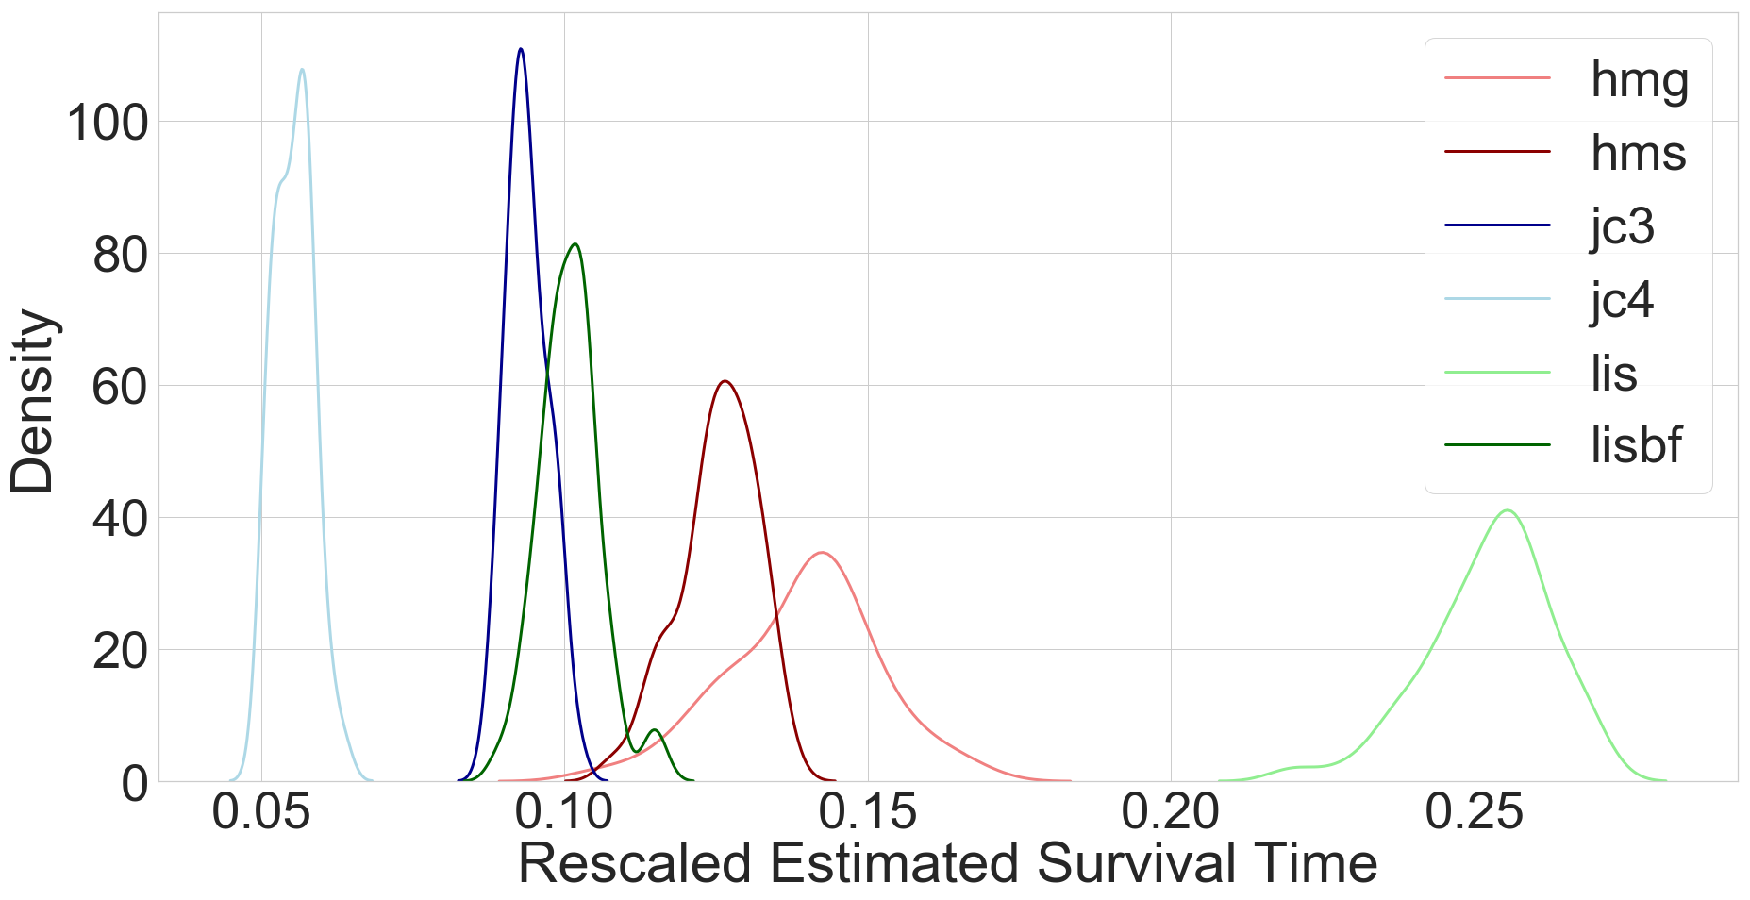
\includegraphics[ width=8.5cm]{images/chapter_3/survival_density_31.pdf}\label{fig:densurv}}
  \hfill
  \subfloat[Churn Probability Predictions]{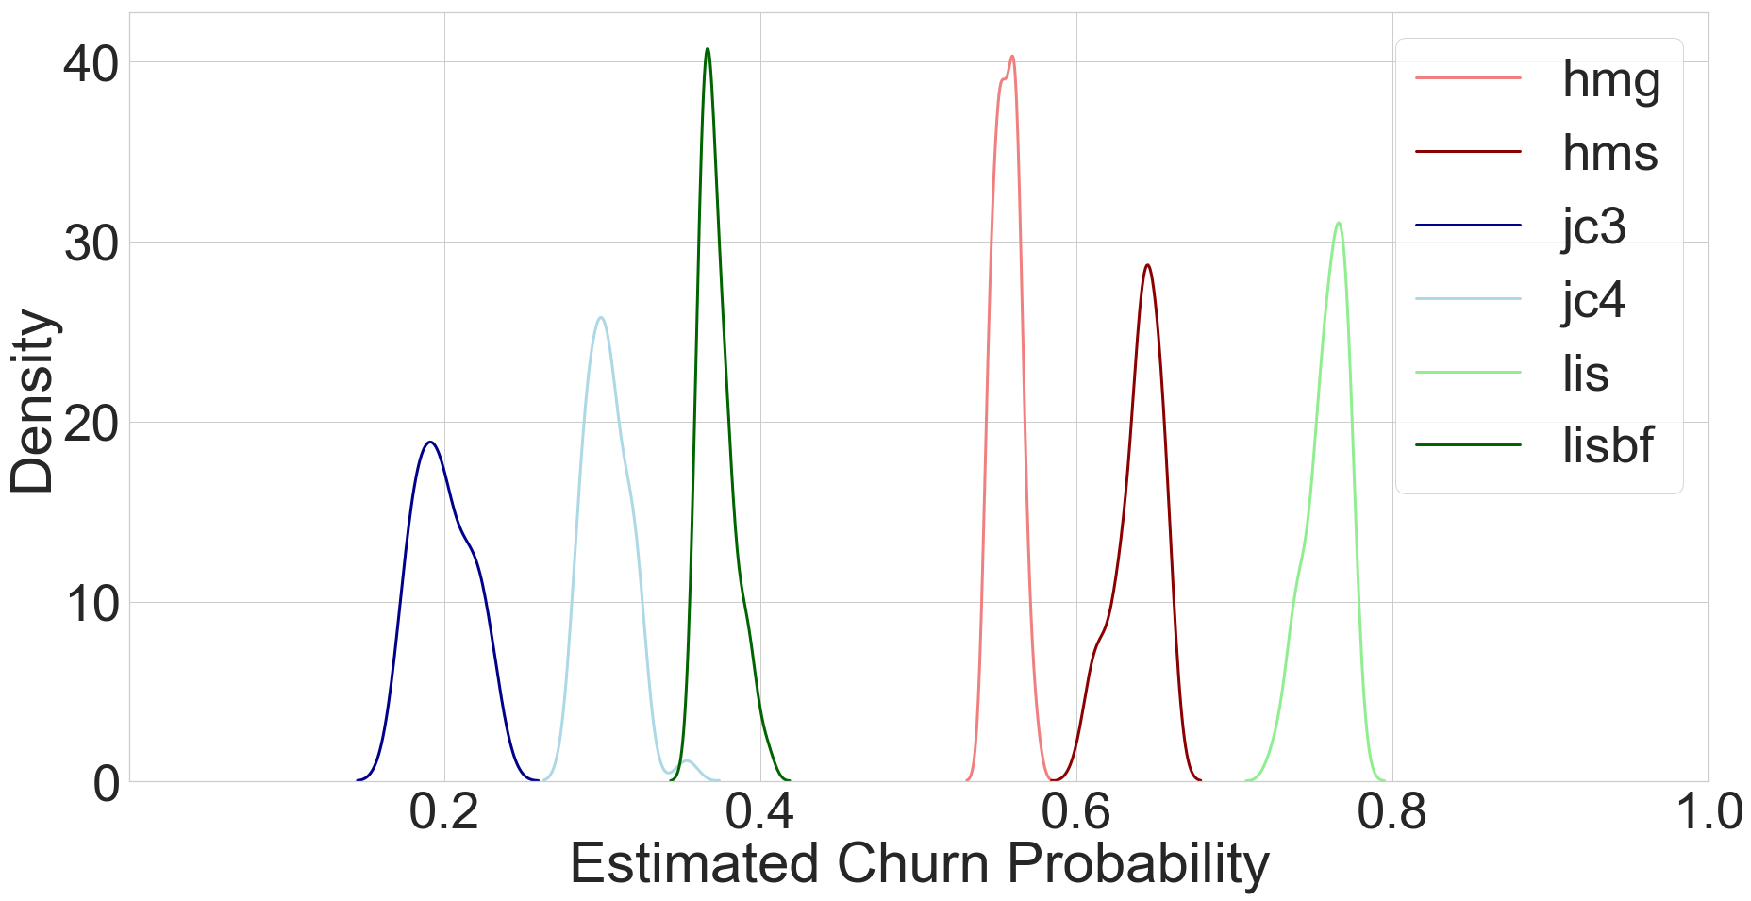
\includegraphics[ width=8.5cm]{images/chapter_3/churn_density_31.pdf}\label{fig:denchurn}}
  \caption[\textbf{Distribution of the BM predictions for six random users, one for each game}]{For better comparison the survival estimates are re-scaled game-wise in the range 0 to 1. The highest density point in the distribution represents the most probable predicted value (i.e. the actual prediction),  while the area under the curve instead can be seen as measure of uncertainty (i.e. how confident is the model in its prediction).}
  \label{distestimations}
\end{figure}
we can see how the model was able to encode different levels of uncertainty in the predicted values through different levels of posterior variance.
\begin{table}[h] \centering
\caption{\textbf{Performance Bifurcating Model}}
\label{bifurcatingperformance}
\resizebox{0.5\textwidth}{!}{
\begin{tabular}{@{}llrr@{}}
\toprule
\textbf{Game}  &\textbf{Models}               & \textbf{SMAPE}      & \textbf{F1}       \\ \midrule
\textbf{hmg}   &\multirow{2}{*}{}             & $27.5 \pm 0.1$   & $0.693 \pm 0.002$ \\
\textbf{hms}   &                              & $20.0 \pm 0.1$   & $0.701 \pm 0.003$ \\
\textbf{jc3}   &\multirow{2}{*}{\textbf{BM}}  & $34.4 \pm 0.3$   & $0.671 \pm 0.005$ \\
\textbf{jc4}   &                              & $32.5 \pm 0.2$   & $0.685 \pm 0.002$ \\
\textbf{lis}   &\multirow{2}{*}{}             & $24.6 \pm 0.2$   & $0.688 \pm 0.003$ \\
\textbf{lisbf} &                              & $20.8 \pm 0.1$   & $0.645 \pm 0.003$ \\ \bottomrule
\end{tabular}
}
\end{table}

\subsection{Model Criticism}
\label{model_criticims_1}
The different level of performance achieved by the baseline model highlighted how different game context proved to be a more challenging ground (e.g. $jc4$ and $lisbf$) than others with respect to the predictive task. Although we did not perform an exhaustive test for evaluating if disjoint models (i.e. models fitted separately to each game context) would outperform our joint modelling approach, we noticed how each parametric model (which all adopt a joint modelling approach) outperformed the baseline(which adopts a disjoint modelling approach) while maintaining a similar performance distribution across game contexts. By looking at the performance of the various parametric models we saw how  the use of models able to capture non-linear interactions between features provided substantial improvements in predicting measures of future behavioural intensity. We also showed that considering the entire history of individual-game interactions provided a consistent but small edge over metrics representations which are collapsed over time. However, this improvement appeared to be markedly more pronounced and consistent when the predictive task was carried out by non-linear models able to take the dynamical nature of the data into account (e.g. the proposed BM architecture). Finally, by looking more in details at the performance of the the BM highlighted how the proposed methodology generalizes well when trying to predict survival time and churn probability as well as successfully incorporating measures of uncertainty in its estimations. In summary, the BM architecture designed following the theoretical principles outlined in chapter \ref{chapter_theory_modelling} showed improved predictive accuracy when compared to alternatives with comparable computational expressiveness (i.e. the MLP architectures). That said, it is evident that the architecture doesn't come fully equipped with all the constrains outlined in chapter \ref{chapter_theory_modelling}
which are necessary for obtaining a good approximation of the type of construct (i.e. attributed incentive salience) presented in the works of McClure et al. \cite{mcclure2003computational} and Zhang et al. \cite{zhang2009neural}. First of all the BM architecture aims at predicting the cumulative expected ammount of future behaviour at an arbitrary early point in time $t \ll T$ (the OP defined in section \ref{model_design_1}) . This implies that, despite the latent representation generated at time $t$ possesses similar predictive powers to attributed incentive salience, these are not on the same time scale and most importantly are not defined for all the $t \in T$. Second despite churn probability and survival time can be considered good approximations of future behavioural intensity, they surely do not fully capture the complexity of the phenomenon. Moreover, these two metrics can be considered of second order (i.e. they are derived from raw quantifiers of behaviour intensity) and artificially created for serving specific concrete applications in the context of engagement quantification. Since the aim of this thesis is to estimate motivation related latent states (from which, as we said in chapter \ref{chapter_lit_review}, the behavioural manifestation of engagement can be directly derived) the next iteration in our model building process focused on modifying the BM architecture in order to make its functional form closer to the specifications highlighted in chapter \ref{chapter_theory_modelling}.

\section{Dynamic Prediction of Future Behavioural Intensity}
\label{model_architecture_2}
In the second iteration of our model building process we focused on improving and expanding the BM architecture in order to increase its flexibility and ability to incorporate the functional constrains specified in chapter \ref{chapter_theory_modelling}. Two major constrains were introduced:
\begin{enumerate}
    \item The new architecture had to jointly predict 5 behavioural metrics. These, differently from churn and survival time, were first order indicator of future behavioural intensity similar to those find in the behavioural neuroscience literature \cite{schultz1997neural,mcclure2003computational,berridge2004motivation,zhang2009neural}
    \item We moved the predictive task from a "static" (i.e. predicting a long-term target after observing a fixed sequence of individual-game interaction) to a "dynamic" one (i.e. performing prediction after each new interaction is observed).
\end{enumerate}
In line with these constrains the experimental task used in this second stage of the model building process aimed at predicting the behavioural intensity of the next interaction between an individual and a videogame after observing an arbitrary number of interactions. More formally, given a sequence of interactions with associated behavioural intensity $B_{t_1 : T}$, the target of the model at any given point in time $t_n$ became
\begin{equation}
\label{joint_target_eq}
   B_{t_{n+1}} = \{B^1_{t_{n+1}}, B^2_{t_{n+1}}, B^3_{t_{n+1}}, B^4_{t_{n+1}}, B^5_{t_{n+1}}\}
\end{equation}
with $\{B^1_{t_{n+1}}, B^2_{t_{n+1}}, B^3_{t_{n+1}}, B^4_{t_{n+1}}, B^5_{t_{n+1}}\}$ being the lead-1 version of the behavioural inputs provided to the model (more details are provided in sections \ref{model_design_2} and \ref{data_2}. This new task is now in line with the formulation presented in section \ref{td_to_supervised} and correspond to predicting the behavioural manifestations of all the phases of the engagement process model \cite{o2008user}, however in a dynamic fashion. The major aim of this second experimental task was to validate the results obtained during the evaluation of the BM architecture while submitting to model constrains that were consistent with the theoretical framework presented in chapter \ref{chapter_lit_review} and \ref{chapter_theory_modelling}. In this view, the hypotheses that we wanted to validate were tightly connected with those presented in section \ref{model_architecture_1}, and had the following form:
\begin{enumerate}
    \item Approaches able to account for non-linear interactions in the considered behavioural metrics can outperform simpler additive models.
    \item The ability to model the type of sequential dynamics presented in section \ref{td_to_supervised} can have a positive effect on the predictive performance.
    \item It is possible to have a single model jointly multiple first-order metrics of behavioural intensity without any substantial loss in accuracy
    \item It is possible to have a single model performing the predictive task simultaneously across a wide range of games.
\end{enumerate}

\subsection{Model Design}
\label{model_design_2}
The second iteration of our ANN architecture was a direct descendant of the BM architecture and aimed to jointly predict a set of 5 behavioural metrics all indicative of the intensity of interactions between an individual and a videogame. Despite being markedly different, the RNN architecture shares similarities with technique used in the neuroscience literature for inferring latent states able to predict observable behaviours \cite{calhoun2019unsupervised}. For example Calhoun et al. used a combination of Hidden Markov Model (HMM) and Generalized Linear Model (GLM) for analyzing the natural behaviour of flies \cite{calhoun2019unsupervised}. Similarly to our proposed architecture, the HMM-GLM approach first infer a latent representation of the observed behaviour though a dynamical model (i.e. HMM) and then uses the same representation for performing predictions using a set of non-linear additive model (i.e. GLM). Our architecture, that we call recurrent (RNN) for simplicity, illustrated in Figure \ref{fig: rnn_2}
\begin{figure}[ht]
\begin{center}
\begin{adjustbox}{width=0.5\textwidth}

   \tikzset{every picture/.style={line width=0.75pt}} %set default line width to 0.75pt        

    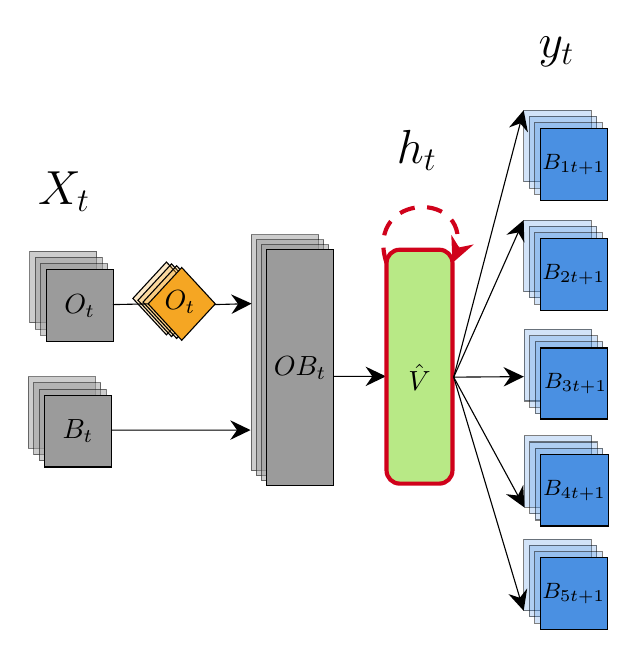
\begin{tikzpicture}[x=0.75pt,y=0.75pt,yscale=-1,xscale=1]
    %uncomment if require: \path (0,354); %set diagram left start at 0, and has height of 354
    
    %Shape: Diamond [id:dp7904557337929367] 
    \draw  [fill={rgb, 255:red, 245; green, 166; blue, 35 }  ,fill opacity=0.25 ] (251.6,119.28) -- (267.77,136.81) -- (251.6,154.33) -- (235.43,136.81) -- cycle ;
    %Shape: Diamond [id:dp44140375398321585] 
    \draw  [fill={rgb, 255:red, 245; green, 166; blue, 35 }  ,fill opacity=0.25 ] (254.05,120.16) -- (270.22,137.68) -- (254.05,155.2) -- (237.89,137.68) -- cycle ;
    %Shape: Diamond [id:dp3808148721846334] 
    \draw  [fill={rgb, 255:red, 245; green, 166; blue, 35 }  ,fill opacity=0.25 ] (256.51,121.04) -- (272.68,138.56) -- (256.51,156.08) -- (240.34,138.56) -- cycle ;
    %Shape: Rectangle [id:dp6212572558437682] 
    \draw  [color={rgb, 255:red, 0; green, 0; blue, 0 }  ,draw opacity=0.5 ][fill={rgb, 255:red, 155; green, 155; blue, 155 }  ,fill opacity=0.5 ] (292.41,106.01) -- (324.92,106.01) -- (324.92,219.74) -- (292.41,219.74) -- cycle ;
    %Shape: Rectangle [id:dp04308865519441296] 
    \draw  [color={rgb, 255:red, 0; green, 0; blue, 0 }  ,draw opacity=0.5 ][fill={rgb, 255:red, 155; green, 155; blue, 155 }  ,fill opacity=0.5 ] (294.86,108.47) -- (327.38,108.47) -- (327.38,222.2) -- (294.86,222.2) -- cycle ;
    %Shape: Rectangle [id:dp692301238884502] 
    \draw  [color={rgb, 255:red, 0; green, 0; blue, 0 }  ,draw opacity=0.5 ][fill={rgb, 255:red, 155; green, 155; blue, 155 }  ,fill opacity=0.5 ] (297.32,110.93) -- (329.84,110.93) -- (329.84,224.66) -- (297.32,224.66) -- cycle ;
    %Shape: Diamond [id:dp3746200743423901] 
    \draw  [fill={rgb, 255:red, 245; green, 166; blue, 35 }  ,fill opacity=1 ] (258.97,121.91) -- (275.13,139.43) -- (258.97,156.96) -- (242.8,139.43) -- cycle ;
    %Straight Lines [id:da9537882301539488] 
    \draw    (274.94,139.77) -- (289.65,139.38) ;
    \draw [shift={(292.65,139.3)}, rotate = 178.49] [fill={rgb, 255:red, 0; green, 0; blue, 0 }  ][line width=0.08]  [draw opacity=0] (9.82,-4.72) -- (0,0) -- (9.82,4.72) -- (6.52,0) -- cycle    ;
    %Straight Lines [id:da45479882207763933] 
    \draw [fill={rgb, 255:red, 155; green, 155; blue, 155 }  ,fill opacity=1 ]   (203.09,200.3) -- (289.13,200.22) ;
    \draw [shift={(292.13,200.22)}, rotate = 179.95] [fill={rgb, 255:red, 0; green, 0; blue, 0 }  ][line width=0.08]  [draw opacity=0] (9.82,-4.72) -- (0,0) -- (9.82,4.72) -- (6.52,0) -- cycle    ;
    %Straight Lines [id:da9952506139878592] 
    \draw [fill={rgb, 255:red, 155; green, 155; blue, 155 }  ,fill opacity=1 ]   (324.42,174.36) -- (354.33,174.35) ;
    \draw [shift={(357.33,174.35)}, rotate = 179.97] [fill={rgb, 255:red, 0; green, 0; blue, 0 }  ][line width=0.08]  [draw opacity=0] (9.82,-4.72) -- (0,0) -- (9.82,4.72) -- (6.52,0) -- cycle    ;
    %Shape: Rectangle [id:dp5105796971723443] 
    \draw  [color={rgb, 255:red, 0; green, 0; blue, 0 }  ,draw opacity=0.5 ][fill={rgb, 255:red, 155; green, 155; blue, 155 }  ,fill opacity=0.5 ] (185.01,174.53) -- (217.26,174.53) -- (217.26,209.05) -- (185.01,209.05) -- cycle ;
    %Shape: Rectangle [id:dp2595806858227925] 
    \draw  [color={rgb, 255:red, 0; green, 0; blue, 0 }  ,draw opacity=0.5 ][fill={rgb, 255:red, 155; green, 155; blue, 155 }  ,fill opacity=0.5 ] (187.63,177.51) -- (219.88,177.51) -- (219.88,212.03) -- (187.63,212.03) -- cycle ;
    %Shape: Rectangle [id:dp8277252726471348] 
    \draw  [color={rgb, 255:red, 0; green, 0; blue, 0 }  ,draw opacity=0.5 ][fill={rgb, 255:red, 155; green, 155; blue, 155 }  ,fill opacity=0.5 ] (190.27,180.56) -- (222.53,180.56) -- (222.53,215.08) -- (190.27,215.08) -- cycle ;
    %Shape: Rectangle [id:dp4311381435790056] 
    \draw  [fill={rgb, 255:red, 155; green, 155; blue, 155 }  ,fill opacity=1 ] (192.86,183.5) -- (225.11,183.5) -- (225.11,218.02) -- (192.86,218.02) -- cycle ;
    %Shape: Rectangle [id:dp5047118561624738] 
    \draw  [fill={rgb, 255:red, 155; green, 155; blue, 155 }  ,fill opacity=1 ] (299.77,113.39) -- (332.29,113.39) -- (332.29,227.12) -- (299.77,227.12) -- cycle ;
    %Shape: Rectangle [id:dp21573647855268596] 
    \draw  [color={rgb, 255:red, 0; green, 0; blue, 0 }  ,draw opacity=0.5 ][fill={rgb, 255:red, 155; green, 155; blue, 155 }  ,fill opacity=0.5 ] (185.83,114.08) -- (218.08,114.08) -- (218.08,148.6) -- (185.83,148.6) -- cycle ;
    %Shape: Rectangle [id:dp8439578107486148] 
    \draw  [color={rgb, 255:red, 0; green, 0; blue, 0 }  ,draw opacity=0.5 ][fill={rgb, 255:red, 155; green, 155; blue, 155 }  ,fill opacity=0.5 ] (188.45,117.06) -- (220.7,117.06) -- (220.7,151.58) -- (188.45,151.58) -- cycle ;
    %Shape: Rectangle [id:dp3660318943838672] 
    \draw  [color={rgb, 255:red, 0; green, 0; blue, 0 }  ,draw opacity=0.5 ][fill={rgb, 255:red, 155; green, 155; blue, 155 }  ,fill opacity=0.5 ] (191.09,120.11) -- (223.35,120.11) -- (223.35,154.63) -- (191.09,154.63) -- cycle ;
    %Shape: Rectangle [id:dp7778058544321894] 
    \draw  [fill={rgb, 255:red, 155; green, 155; blue, 155 }  ,fill opacity=1 ] (193.68,123.05) -- (225.93,123.05) -- (225.93,157.57) -- (193.68,157.57) -- cycle ;
    %Straight Lines [id:da7015539931476137] 
    \draw    (225.82,139.77) -- (242.8,139.43) ;
    %Rounded Rect [id:dp4473399888202214] 
    \draw  [color={rgb, 255:red, 208; green, 2; blue, 27 }  ,draw opacity=1 ][fill={rgb, 255:red, 184; green, 233; blue, 134 }  ,fill opacity=1 ][line width=1.5]  (357.64,119.69) .. controls (357.64,116.18) and (360.48,113.34) .. (363.99,113.34) -- (383.05,113.34) .. controls (386.56,113.34) and (389.4,116.18) .. (389.4,119.69) -- (389.4,219.68) .. controls (389.4,223.19) and (386.56,226.03) .. (383.05,226.03) -- (363.99,226.03) .. controls (360.48,226.03) and (357.64,223.19) .. (357.64,219.68) -- cycle ;
    %Curve Lines [id:da30430836514862303] 
    \draw [color={rgb, 255:red, 208; green, 2; blue, 27 }  ,draw opacity=1 ][line width=1.5]  [dash pattern={on 5.63pt off 4.5pt}]  (357.64,119.69) .. controls (346.28,85.07) and (400.82,83.85) .. (390.76,116.05) ;
    \draw [shift={(389.4,119.69)}, rotate = 293.32] [fill={rgb, 255:red, 208; green, 2; blue, 27 }  ,fill opacity=1 ][line width=0.08]  [draw opacity=0] (12.23,-5.88) -- (0,0) -- (12.23,5.88) -- (8.12,0) -- cycle    ;
    %Shape: Rectangle [id:dp9161667828288995] 
    \draw  [color={rgb, 255:red, 0; green, 0; blue, 0 }  ,draw opacity=0.5 ][fill={rgb, 255:red, 74; green, 144; blue, 226 }  ,fill opacity=0.25 ] (423.7,99.06) -- (456.2,99.06) -- (456.2,133.57) -- (423.7,133.57) -- cycle ;
    %Shape: Rectangle [id:dp20889912329934768] 
    \draw  [color={rgb, 255:red, 0; green, 0; blue, 0 }  ,draw opacity=0.5 ][fill={rgb, 255:red, 74; green, 144; blue, 226 }  ,fill opacity=0.25 ] (426.34,102.04) -- (458.84,102.04) -- (458.84,136.54) -- (426.34,136.54) -- cycle ;
    %Shape: Rectangle [id:dp2816776467625347] 
    \draw  [color={rgb, 255:red, 0; green, 0; blue, 0 }  ,draw opacity=0.5 ][fill={rgb, 255:red, 74; green, 144; blue, 226 }  ,fill opacity=0.25 ] (429,105.09) -- (461.51,105.09) -- (461.51,139.6) -- (429,139.6) -- cycle ;
    %Shape: Rectangle [id:dp42330781005921503] 
    \draw  [fill={rgb, 255:red, 74; green, 144; blue, 226 }  ,fill opacity=1 ] (431.61,108.03) -- (464.11,108.03) -- (464.11,142.53) -- (431.61,142.53) -- cycle ;
    %Shape: Rectangle [id:dp687693866282439] 
    \draw  [color={rgb, 255:red, 0; green, 0; blue, 0 }  ,draw opacity=0.5 ][fill={rgb, 255:red, 74; green, 144; blue, 226 }  ,fill opacity=0.25 ] (424.03,151.72) -- (456.53,151.72) -- (456.53,186.23) -- (424.03,186.23) -- cycle ;
    %Shape: Rectangle [id:dp48312027278133507] 
    \draw  [color={rgb, 255:red, 0; green, 0; blue, 0 }  ,draw opacity=0.5 ][fill={rgb, 255:red, 74; green, 144; blue, 226 }  ,fill opacity=0.25 ] (426.67,154.7) -- (459.17,154.7) -- (459.17,189.21) -- (426.67,189.21) -- cycle ;
    %Shape: Rectangle [id:dp5685283982245644] 
    \draw  [color={rgb, 255:red, 0; green, 0; blue, 0 }  ,draw opacity=0.5 ][fill={rgb, 255:red, 74; green, 144; blue, 226 }  ,fill opacity=0.25 ] (429.33,157.76) -- (461.84,157.76) -- (461.84,192.26) -- (429.33,192.26) -- cycle ;
    %Shape: Rectangle [id:dp3612684141121718] 
    \draw  [fill={rgb, 255:red, 74; green, 144; blue, 226 }  ,fill opacity=1 ] (431.95,160.69) -- (464.17,160.69) -- (464.17,194.89) -- (431.95,194.89) -- cycle ;
    %Shape: Rectangle [id:dp17418879327554693] 
    \draw  [color={rgb, 255:red, 0; green, 0; blue, 0 }  ,draw opacity=0.5 ][fill={rgb, 255:red, 74; green, 144; blue, 226 }  ,fill opacity=0.25 ] (423.7,252.78) -- (456.2,252.78) -- (456.2,287.29) -- (423.7,287.29) -- cycle ;
    %Shape: Rectangle [id:dp6752714184560265] 
    \draw  [color={rgb, 255:red, 0; green, 0; blue, 0 }  ,draw opacity=0.5 ][fill={rgb, 255:red, 74; green, 144; blue, 226 }  ,fill opacity=0.25 ] (426.34,255.76) -- (458.84,255.76) -- (458.84,290.26) -- (426.34,290.26) -- cycle ;
    %Shape: Rectangle [id:dp9983191940012098] 
    \draw  [color={rgb, 255:red, 0; green, 0; blue, 0 }  ,draw opacity=0.5 ][fill={rgb, 255:red, 74; green, 144; blue, 226 }  ,fill opacity=0.25 ] (429,258.81) -- (461.51,258.81) -- (461.51,293.32) -- (429,293.32) -- cycle ;
    %Shape: Rectangle [id:dp11003700320217247] 
    \draw  [fill={rgb, 255:red, 74; green, 144; blue, 226 }  ,fill opacity=1 ] (431.61,261.75) -- (464.11,261.75) -- (464.11,296.25) -- (431.61,296.25) -- cycle ;
    %Shape: Rectangle [id:dp7367493878137299] 
    \draw  [color={rgb, 255:red, 0; green, 0; blue, 0 }  ,draw opacity=0.5 ][fill={rgb, 255:red, 74; green, 144; blue, 226 }  ,fill opacity=0.25 ] (424.03,202.99) -- (456.53,202.99) -- (456.53,237.5) -- (424.03,237.5) -- cycle ;
    %Shape: Rectangle [id:dp8983348276713422] 
    \draw  [color={rgb, 255:red, 0; green, 0; blue, 0 }  ,draw opacity=0.5 ][fill={rgb, 255:red, 74; green, 144; blue, 226 }  ,fill opacity=0.25 ] (426.67,205.97) -- (459.17,205.97) -- (459.17,240.47) -- (426.67,240.47) -- cycle ;
    %Shape: Rectangle [id:dp09933660328753013] 
    \draw  [color={rgb, 255:red, 0; green, 0; blue, 0 }  ,draw opacity=0.5 ][fill={rgb, 255:red, 74; green, 144; blue, 226 }  ,fill opacity=0.25 ] (429.33,209.02) -- (461.84,209.02) -- (461.84,243.53) -- (429.33,243.53) -- cycle ;
    %Shape: Rectangle [id:dp9943795167198757] 
    \draw  [fill={rgb, 255:red, 74; green, 144; blue, 226 }  ,fill opacity=1 ] (431.94,211.96) -- (464.44,211.96) -- (464.44,246.46) -- (431.94,246.46) -- cycle ;
    %Shape: Rectangle [id:dp058820430549127] 
    \draw  [color={rgb, 255:red, 0; green, 0; blue, 0 }  ,draw opacity=0.5 ][fill={rgb, 255:red, 74; green, 144; blue, 226 }  ,fill opacity=0.25 ] (423.7,46.14) -- (456.2,46.14) -- (456.2,80.65) -- (423.7,80.65) -- cycle ;
    %Shape: Rectangle [id:dp9593581977954196] 
    \draw  [color={rgb, 255:red, 0; green, 0; blue, 0 }  ,draw opacity=0.5 ][fill={rgb, 255:red, 74; green, 144; blue, 226 }  ,fill opacity=0.25 ] (426.34,49.12) -- (458.84,49.12) -- (458.84,83.63) -- (426.34,83.63) -- cycle ;
    %Shape: Rectangle [id:dp4362593009406618] 
    \draw  [color={rgb, 255:red, 0; green, 0; blue, 0 }  ,draw opacity=0.5 ][fill={rgb, 255:red, 74; green, 144; blue, 226 }  ,fill opacity=0.25 ] (429,52.17) -- (461.51,52.17) -- (461.51,86.68) -- (429,86.68) -- cycle ;
    %Shape: Rectangle [id:dp7619519997532663] 
    \draw  [fill={rgb, 255:red, 74; green, 144; blue, 226 }  ,fill opacity=1 ] (431.61,55.11) -- (464.11,55.11) -- (464.11,89.62) -- (431.61,89.62) -- cycle ;
    %Straight Lines [id:da545267197618029] 
    \draw    (390,174.73) -- (422.94,49.05) ;
    \draw [shift={(423.7,46.14)}, rotate = 104.68] [fill={rgb, 255:red, 0; green, 0; blue, 0 }  ][line width=0.08]  [draw opacity=0] (9.82,-4.72) -- (0,0) -- (9.82,4.72) -- (6.52,0) -- cycle    ;
    %Straight Lines [id:da9271821433537066] 
    \draw    (390,174.73) -- (422.48,101.8) ;
    \draw [shift={(423.7,99.06)}, rotate = 114] [fill={rgb, 255:red, 0; green, 0; blue, 0 }  ][line width=0.08]  [draw opacity=0] (9.82,-4.72) -- (0,0) -- (9.82,4.72) -- (6.52,0) -- cycle    ;
    %Straight Lines [id:da6232303168074279] 
    \draw    (390,174.73) -- (420.8,174.5) ;
    \draw [shift={(423.8,174.48)}, rotate = 179.57] [fill={rgb, 255:red, 0; green, 0; blue, 0 }  ][line width=0.08]  [draw opacity=0] (9.82,-4.72) -- (0,0) -- (9.82,4.72) -- (6.52,0) -- cycle    ;
    %Straight Lines [id:da1424758683168187] 
    \draw    (390,174.73) -- (422.6,234.86) ;
    \draw [shift={(424.03,237.5)}, rotate = 241.54] [fill={rgb, 255:red, 0; green, 0; blue, 0 }  ][line width=0.08]  [draw opacity=0] (9.82,-4.72) -- (0,0) -- (9.82,4.72) -- (6.52,0) -- cycle    ;
    %Straight Lines [id:da40105840572004403] 
    \draw    (390,174.73) -- (422.84,284.41) ;
    \draw [shift={(423.7,287.29)}, rotate = 253.33] [fill={rgb, 255:red, 0; green, 0; blue, 0 }  ][line width=0.08]  [draw opacity=0] (9.82,-4.72) -- (0,0) -- (9.82,4.72) -- (6.52,0) -- cycle    ;
    
    % Text Node
    \draw (208.99,200.76) node  [font=\normalsize]  {$B_{t}$};
    % Text Node
    \draw (373.52,174.8) node  [font=\normalsize]  {$\hat{V}$};
    % Text Node
    \draw (258.15,138.56) node  [font=\normalsize]  {$O_{t}$};
    % Text Node
    \draw (202.34,85.25) node  [font=\LARGE]  {$X_{t}$};
    % Text Node
    \draw (316.03,170.25) node  [font=\normalsize]  {$OB_{t}$};
    % Text Node
    \draw (209.81,140.31) node  [font=\normalsize]  {$O_{t}$};
    % Text Node
    \draw (372.34,65.6) node  [font=\LARGE]  {$h_{t}$};
    % Text Node
    \draw (447.86,125.28) node  [font=\footnotesize]  {$B_{2t+1}$};
    % Text Node
    \draw (448.74,177.94) node  [font=\footnotesize]  {$B_{3t+1}$};
    % Text Node
    \draw (448.19,229.21) node  [font=\footnotesize]  {$B_{4t+1}$};
    % Text Node
    \draw (447.86,279) node  [font=\footnotesize]  {$B_{5t+1}$};
    % Text Node
    \draw (439.54,18) node  [font=\LARGE]  {$y_{t}$};
    % Text Node
    \draw (447.86,72.36) node  [font=\footnotesize]  {$B_{1t+1}$};
    
    
    \end{tikzpicture}


\end{adjustbox}
\end{center}
\caption[\textbf{The recurrent architecture}]{Blue, orange and green shapes represent respectively feedforward, embedding and LSTM operations. Gray shapes indicate operations with no learnable parameters, such as tensor instantiation and concatenation. Stacked, transparent colouring indicates tensors with a sequential structure. Straight and curved arrows refer to the presence of feed-forward or recurrent information flow. The red highlight shows the portion of the model we hypothesize is inferring an approximation of attributed incentive salience.}
\label{fig: rnn_2}
\end{figure}
extend the work of Calhoun et al. by removing the additive and markovian assumptions and by dropping the requirement for a fixed number of hidden states. The model receives the same input of the architecture described in section \ref{model_design_2} with the major difference that no padding was required. Indeed we decided to exploit the ability of RNN to flexibly fit variable-length time series and opted for a data generator approach \footnote{See \cite{chollet2015keras,tensorflow2015-whitepaper} for implementation details.}, feeding data to the models in random batches with constant length within a batch. The type of operations performed by the architecture were identical to those presented in section \ref{model_design_1} although with 2 major differences. First, the RNN component of the architecture was now of type many-to-many therefore producing an $H \in \mathbb{R}^{N \times T \times h}$ tensor constituting the sequence of hidden states produced by the LSTM operation after observing each element of the input time series\cite{bengio2017deep}. Second, the final step of the architecture now exploits the temporal nature of the latent representation generated by the RNN for predicting not just a single value but a sequence of values, namely the lead-1 version of the input time series. This was again achieved by means of multi-task learning with five ANNs with fully connected operations. In order to apply the fully connected operations to a sequence of latent states we distributed their computations across time \footnote{See \cite{chollet2015keras} for implementation details} (see Appendix \ref{time_distributed}) so that each ANN could produce a tensor of shape $\hat{y} \in \mathbb{R}^{N \times T \times 1}$. We want to highlight that the model now fully reflect the formulation presented in section \ref{td_to_supervised}, indeed if again we look at the representations generated by the LSTM in terms of target expectation
\begin{gather}
\label{rnn_1_exp}
   h_t = f^1(O, B_{t}, h_{t-1}; \theta^1)  \\ \nonumber
   \mathbb{E}[B_{t+1}] = f^2(h_t; \theta^2) \\ \nonumber    
\end{gather}
we can can see how at each point in time the generated representation $h_t$ is mostly indicative of the behavioural intensity a time $t+1$ but it also needs to retain some predictive power for all the subsequent time steps. The model used a combination of $ReLU$, $ELU$ and $LReLU$ (see Appendix \ref{elu} and \ref{lelu}) as activations functions for the hidden units (more details on their selection are specified in \ref{tuning_comparison_2} whereas the link function used for generating the prediction was always the $identity$ function. As a regularization strategy we decided to drop the use of batch normalization, as it proved challenging to adopt with a multivariate time-series target, and introduces a variant of dropout (i.e. One Dimensional Spatial Dropout see Appendix \ref{spatial_dropout}) more suitable for time series data and applied it after each layer in the architecture.

\paragraph{Competing Models}
\label{competing_models_2}
As in the previous stage of the model building process a series of competing models were implemented for testing our hypotheses. First, we decided to improve our baseline by establishing two reasonable single-parameter models. The first is a Lag 1 model producing predictions according to the following rule:
\begin{equation}
   \begin{gathered}  
     B_{t+1} = B_{t}
     \label{lag_1}
  \end{gathered}
\end{equation}
here $t$ represent a single game session in a sequence of $T$ observed interactions while $B$ are the same behavioural metrics the RNN model recives as input (they are thoroughly described in section \ref{data_2}). The second is a Median model computing the expectation of each of the 5 targets according to the formula:
\begin{equation}
  \begin{gathered}  
    \overline{B_{t+1}} = \frac
      {\sum_{i=1}^{t+1} wB_{i}}
      {\sum_{i=1}^{t+1} w }\\
    B_{t+1} = median(\overline{B_{t+1}}) 
    \label{median}
  \end{gathered}
\end{equation}
here $\overline{B_{t+1}}$ is an exponentially weighted average of all the $B_t$ up to $t+1$ observed when fitting the model. This is computed separately for every individual in the dataset and the median value of each of the 5 targets is used a a constant prediction. These apparently naive models provide a surprisingly robust prediction baseline for time series that are not white noise \cite{hyndman2018forecasting} other than having a nice interpretation in terms of behavioural momentum \cite{nevin2000behavioral}: in conditions of high experienced reward the behaviour of an individual tends to be consistent over time (i.e. resistant to change). Similarly to the model used in the assessment of the BM architecture, a multi-task linear model with Elastic-Net regularization (ENet) \cite{zou2005regularization} was used to evaluate the performance of simple additive models. While for testing the effect of non linearity, a multi-task Multilayer Perceptron (MLP) was employed. Both model used an embedding operation for encoding information from the game context but the ENet model had the number of hidden units fixed to 1 an relied on an $identity$ activation function. This was done for avoiding to introduce non-linearity in the ENet model. Figure \ref{fig: mlp_2} show the architecture used for both the ENet and MLP models. We can see that differently from the models used in section \ref{model_architecture_1} the only difference with RNN architecture lies in the use of time distributed fully connected operations instead of those provided by the LSTM. 
\begin{figure}[ht]
\begin{center}
\begin{adjustbox}{width=0.7\textwidth}

\tikzset{every picture/.style={line width=0.75pt}} %set default line width to 0.75pt        

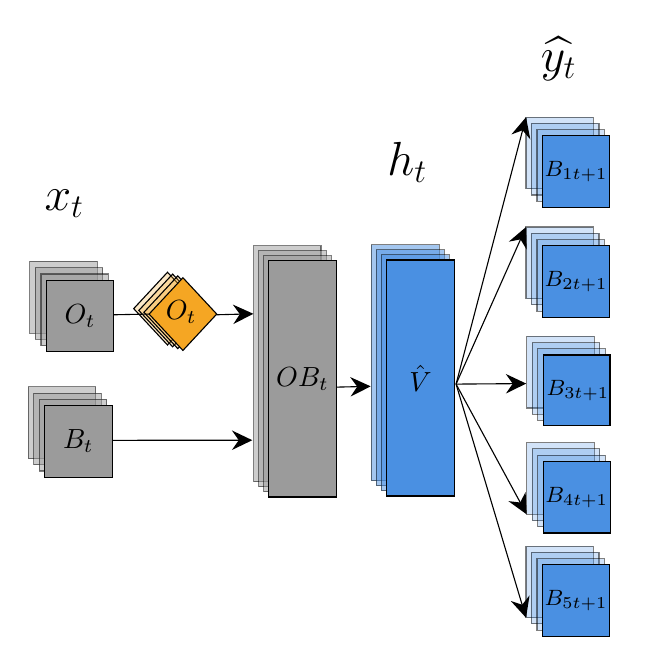
\begin{tikzpicture}[x=0.75pt,y=0.75pt,yscale=-1,xscale=1]
%uncomment if require: \path (0,331); %set diagram left start at 0, and has height of 331

%Shape: Diamond [id:dp8512741780313259] 
\draw  [fill={rgb, 255:red, 245; green, 166; blue, 35 }  ,fill opacity=0.25 ] (257.97,138.57) -- (274.27,156.09) -- (257.97,173.6) -- (241.68,156.09) -- cycle ;
%Shape: Diamond [id:dp44131568061643844] 
\draw  [fill={rgb, 255:red, 245; green, 166; blue, 35 }  ,fill opacity=0.25 ] (260.45,139.45) -- (276.74,156.96) -- (260.45,174.48) -- (244.15,156.96) -- cycle ;
%Shape: Diamond [id:dp9944377463655836] 
\draw  [fill={rgb, 255:red, 245; green, 166; blue, 35 }  ,fill opacity=0.25 ] (262.92,140.32) -- (279.22,157.84) -- (262.92,175.35) -- (246.63,157.84) -- cycle ;
%Shape: Rectangle [id:dp3605470636117536] 
\draw  [color={rgb, 255:red, 0; green, 0; blue, 0 }  ,draw opacity=0.5 ][fill={rgb, 255:red, 74; green, 144; blue, 226 }  ,fill opacity=0.5 ] (356.1,125.3) -- (388.87,125.3) -- (388.87,239) -- (356.1,239) -- cycle ;
%Shape: Rectangle [id:dp7194333726509892] 
\draw  [color={rgb, 255:red, 0; green, 0; blue, 0 }  ,draw opacity=0.5 ][fill={rgb, 255:red, 74; green, 144; blue, 226 }  ,fill opacity=0.5 ] (358.57,127.76) -- (391.34,127.76) -- (391.34,241.46) -- (358.57,241.46) -- cycle ;
%Shape: Rectangle [id:dp3276084138933598] 
\draw  [color={rgb, 255:red, 0; green, 0; blue, 0 }  ,draw opacity=0.5 ][fill={rgb, 255:red, 74; green, 144; blue, 226 }  ,fill opacity=0.5 ] (361.05,130.22) -- (393.82,130.22) -- (393.82,243.92) -- (361.05,243.92) -- cycle ;
%Shape: Diamond [id:dp6965315978812838] 
\draw  [fill={rgb, 255:red, 245; green, 166; blue, 35 }  ,fill opacity=1 ] (265.4,141.2) -- (281.69,158.71) -- (265.4,176.23) -- (249.1,158.71) -- cycle ;
%Straight Lines [id:da5408632178702979] 
\draw    (281.5,159.05) -- (296.35,158.66) ;
\draw [shift={(299.35,158.58)}, rotate = 178.5] [fill={rgb, 255:red, 0; green, 0; blue, 0 }  ][line width=0.08]  [draw opacity=0] (9.82,-4.72) -- (0,0) -- (9.82,4.72) -- (6.52,0) -- cycle    ;
%Straight Lines [id:da38550305545794683] 
\draw [fill={rgb, 255:red, 155; green, 155; blue, 155 }  ,fill opacity=1 ]   (209.09,219.56) -- (295.82,219.48) ;
\draw [shift={(298.82,219.48)}, rotate = 179.95] [fill={rgb, 255:red, 0; green, 0; blue, 0 }  ][line width=0.08]  [draw opacity=0] (9.82,-4.72) -- (0,0) -- (9.82,4.72) -- (6.52,0) -- cycle    ;
%Shape: Rectangle [id:dp8586026364143547] 
\draw  [color={rgb, 255:red, 0; green, 0; blue, 0 }  ,draw opacity=0.5 ][fill={rgb, 255:red, 74; green, 144; blue, 226 }  ,fill opacity=0.25 ] (430.7,116.78) -- (463.2,116.78) -- (463.2,151.29) -- (430.7,151.29) -- cycle ;
%Shape: Rectangle [id:dp5271658440371366] 
\draw  [color={rgb, 255:red, 0; green, 0; blue, 0 }  ,draw opacity=0.5 ][fill={rgb, 255:red, 74; green, 144; blue, 226 }  ,fill opacity=0.25 ] (433.34,119.76) -- (465.84,119.76) -- (465.84,154.27) -- (433.34,154.27) -- cycle ;
%Shape: Rectangle [id:dp6121896210605144] 
\draw  [color={rgb, 255:red, 0; green, 0; blue, 0 }  ,draw opacity=0.5 ][fill={rgb, 255:red, 74; green, 144; blue, 226 }  ,fill opacity=0.25 ] (436,122.81) -- (468.51,122.81) -- (468.51,157.32) -- (436,157.32) -- cycle ;
%Shape: Rectangle [id:dp2571940122217342] 
\draw  [fill={rgb, 255:red, 74; green, 144; blue, 226 }  ,fill opacity=1 ] (438.61,125.75) -- (471.11,125.75) -- (471.11,160.25) -- (438.61,160.25) -- cycle ;
%Shape: Rectangle [id:dp04921858860159267] 
\draw  [color={rgb, 255:red, 0; green, 0; blue, 0 }  ,draw opacity=0.5 ][fill={rgb, 255:red, 74; green, 144; blue, 226 }  ,fill opacity=0.25 ] (431.03,169.45) -- (463.53,169.45) -- (463.53,203.95) -- (431.03,203.95) -- cycle ;
%Shape: Rectangle [id:dp5512084563866699] 
\draw  [color={rgb, 255:red, 0; green, 0; blue, 0 }  ,draw opacity=0.5 ][fill={rgb, 255:red, 74; green, 144; blue, 226 }  ,fill opacity=0.25 ] (433.67,172.43) -- (466.17,172.43) -- (466.17,206.93) -- (433.67,206.93) -- cycle ;
%Shape: Rectangle [id:dp948946889597384] 
\draw  [color={rgb, 255:red, 0; green, 0; blue, 0 }  ,draw opacity=0.5 ][fill={rgb, 255:red, 74; green, 144; blue, 226 }  ,fill opacity=0.25 ] (436.33,175.48) -- (468.84,175.48) -- (468.84,209.98) -- (436.33,209.98) -- cycle ;
%Shape: Rectangle [id:dp7446725750615967] 
\draw  [fill={rgb, 255:red, 74; green, 144; blue, 226 }  ,fill opacity=1 ] (438.95,178.41) -- (471.17,178.41) -- (471.17,212.61) -- (438.95,212.61) -- cycle ;
%Shape: Rectangle [id:dp2953756097578333] 
\draw  [color={rgb, 255:red, 0; green, 0; blue, 0 }  ,draw opacity=0.5 ][fill={rgb, 255:red, 74; green, 144; blue, 226 }  ,fill opacity=0.25 ] (430.7,270.5) -- (463.2,270.5) -- (463.2,305.01) -- (430.7,305.01) -- cycle ;
%Shape: Rectangle [id:dp8190984811103563] 
\draw  [color={rgb, 255:red, 0; green, 0; blue, 0 }  ,draw opacity=0.5 ][fill={rgb, 255:red, 74; green, 144; blue, 226 }  ,fill opacity=0.25 ] (433.34,273.48) -- (465.84,273.48) -- (465.84,307.99) -- (433.34,307.99) -- cycle ;
%Shape: Rectangle [id:dp1989563986467071] 
\draw  [color={rgb, 255:red, 0; green, 0; blue, 0 }  ,draw opacity=0.5 ][fill={rgb, 255:red, 74; green, 144; blue, 226 }  ,fill opacity=0.25 ] (436,276.53) -- (468.51,276.53) -- (468.51,311.04) -- (436,311.04) -- cycle ;
%Shape: Rectangle [id:dp1924397511107222] 
\draw  [fill={rgb, 255:red, 74; green, 144; blue, 226 }  ,fill opacity=1 ] (438.61,279.47) -- (471.11,279.47) -- (471.11,313.98) -- (438.61,313.98) -- cycle ;
%Shape: Rectangle [id:dp8187051960536611] 
\draw  [color={rgb, 255:red, 0; green, 0; blue, 0 }  ,draw opacity=0.5 ][fill={rgb, 255:red, 74; green, 144; blue, 226 }  ,fill opacity=0.25 ] (431.03,220.71) -- (463.53,220.71) -- (463.53,255.22) -- (431.03,255.22) -- cycle ;
%Shape: Rectangle [id:dp6023578581008111] 
\draw  [color={rgb, 255:red, 0; green, 0; blue, 0 }  ,draw opacity=0.5 ][fill={rgb, 255:red, 74; green, 144; blue, 226 }  ,fill opacity=0.25 ] (433.67,223.69) -- (466.17,223.69) -- (466.17,258.2) -- (433.67,258.2) -- cycle ;
%Shape: Rectangle [id:dp8798703561171738] 
\draw  [color={rgb, 255:red, 0; green, 0; blue, 0 }  ,draw opacity=0.5 ][fill={rgb, 255:red, 74; green, 144; blue, 226 }  ,fill opacity=0.25 ] (436.33,226.74) -- (468.84,226.74) -- (468.84,261.25) -- (436.33,261.25) -- cycle ;
%Shape: Rectangle [id:dp3283044450373016] 
\draw  [fill={rgb, 255:red, 74; green, 144; blue, 226 }  ,fill opacity=1 ] (438.94,229.68) -- (471.44,229.68) -- (471.44,264.19) -- (438.94,264.19) -- cycle ;
%Shape: Rectangle [id:dp15154204076473643] 
\draw  [color={rgb, 255:red, 0; green, 0; blue, 0 }  ,draw opacity=0.5 ][fill={rgb, 255:red, 155; green, 155; blue, 155 }  ,fill opacity=0.5 ] (190.87,193.8) -- (223.37,193.8) -- (223.37,228.31) -- (190.87,228.31) -- cycle ;
%Shape: Rectangle [id:dp9182207029607203] 
\draw  [color={rgb, 255:red, 0; green, 0; blue, 0 }  ,draw opacity=0.5 ][fill={rgb, 255:red, 155; green, 155; blue, 155 }  ,fill opacity=0.5 ] (193.51,196.78) -- (226.01,196.78) -- (226.01,231.28) -- (193.51,231.28) -- cycle ;
%Shape: Rectangle [id:dp7698171692832448] 
\draw  [color={rgb, 255:red, 0; green, 0; blue, 0 }  ,draw opacity=0.5 ][fill={rgb, 255:red, 155; green, 155; blue, 155 }  ,fill opacity=0.5 ] (196.17,199.83) -- (228.68,199.83) -- (228.68,234.34) -- (196.17,234.34) -- cycle ;
%Shape: Rectangle [id:dp3865383455450443] 
\draw  [fill={rgb, 255:red, 155; green, 155; blue, 155 }  ,fill opacity=1 ] (198.78,202.77) -- (231.28,202.77) -- (231.28,237.27) -- (198.78,237.27) -- cycle ;
%Shape: Rectangle [id:dp23172130161456372] 
\draw  [fill={rgb, 255:red, 74; green, 144; blue, 226 }  ,fill opacity=1 ] (363.52,132.67) -- (396.29,132.67) -- (396.29,246.37) -- (363.52,246.37) -- cycle ;
%Shape: Rectangle [id:dp18125329077839125] 
\draw  [color={rgb, 255:red, 0; green, 0; blue, 0 }  ,draw opacity=0.5 ][fill={rgb, 255:red, 74; green, 144; blue, 226 }  ,fill opacity=0.25 ] (430.7,63.87) -- (463.2,63.87) -- (463.2,98.37) -- (430.7,98.37) -- cycle ;
%Shape: Rectangle [id:dp3729389269249752] 
\draw  [color={rgb, 255:red, 0; green, 0; blue, 0 }  ,draw opacity=0.5 ][fill={rgb, 255:red, 74; green, 144; blue, 226 }  ,fill opacity=0.25 ] (433.34,66.84) -- (465.84,66.84) -- (465.84,101.35) -- (433.34,101.35) -- cycle ;
%Shape: Rectangle [id:dp8889532693849542] 
\draw  [color={rgb, 255:red, 0; green, 0; blue, 0 }  ,draw opacity=0.5 ][fill={rgb, 255:red, 74; green, 144; blue, 226 }  ,fill opacity=0.25 ] (436,69.9) -- (468.51,69.9) -- (468.51,104.4) -- (436,104.4) -- cycle ;
%Shape: Rectangle [id:dp22768677359456946] 
\draw  [fill={rgb, 255:red, 74; green, 144; blue, 226 }  ,fill opacity=1 ] (438.61,72.83) -- (471.11,72.83) -- (471.11,107.34) -- (438.61,107.34) -- cycle ;
%Straight Lines [id:da6521632540749734] 
\draw    (397,192.45) -- (429.94,66.77) ;
\draw [shift={(430.7,63.87)}, rotate = 104.68] [fill={rgb, 255:red, 0; green, 0; blue, 0 }  ][line width=0.08]  [draw opacity=0] (9.82,-4.72) -- (0,0) -- (9.82,4.72) -- (6.52,0) -- cycle    ;
%Straight Lines [id:da4098284445759105] 
\draw    (397,192.45) -- (429.48,119.52) ;
\draw [shift={(430.7,116.78)}, rotate = 114] [fill={rgb, 255:red, 0; green, 0; blue, 0 }  ][line width=0.08]  [draw opacity=0] (9.82,-4.72) -- (0,0) -- (9.82,4.72) -- (6.52,0) -- cycle    ;
%Straight Lines [id:da6632019398295455] 
\draw    (397,192.45) -- (427.8,192.22) ;
\draw [shift={(430.8,192.2)}, rotate = 179.57] [fill={rgb, 255:red, 0; green, 0; blue, 0 }  ][line width=0.08]  [draw opacity=0] (9.82,-4.72) -- (0,0) -- (9.82,4.72) -- (6.52,0) -- cycle    ;
%Straight Lines [id:da3742350341861914] 
\draw    (397,192.45) -- (429.6,252.58) ;
\draw [shift={(431.03,255.22)}, rotate = 241.54] [fill={rgb, 255:red, 0; green, 0; blue, 0 }  ][line width=0.08]  [draw opacity=0] (9.82,-4.72) -- (0,0) -- (9.82,4.72) -- (6.52,0) -- cycle    ;
%Straight Lines [id:da8736791937763184] 
\draw    (397,192.45) -- (429.84,302.14) ;
\draw [shift={(430.7,305.01)}, rotate = 253.33] [fill={rgb, 255:red, 0; green, 0; blue, 0 }  ][line width=0.08]  [draw opacity=0] (9.82,-4.72) -- (0,0) -- (9.82,4.72) -- (6.52,0) -- cycle    ;
%Shape: Rectangle [id:dp20286680685222525] 
\draw  [color={rgb, 255:red, 0; green, 0; blue, 0 }  ,draw opacity=0.5 ][fill={rgb, 255:red, 155; green, 155; blue, 155 }  ,fill opacity=0.5 ] (191.69,133.37) -- (224.2,133.37) -- (224.2,167.88) -- (191.69,167.88) -- cycle ;
%Shape: Rectangle [id:dp3612691236911778] 
\draw  [color={rgb, 255:red, 0; green, 0; blue, 0 }  ,draw opacity=0.5 ][fill={rgb, 255:red, 155; green, 155; blue, 155 }  ,fill opacity=0.5 ] (194.33,136.35) -- (226.84,136.35) -- (226.84,170.85) -- (194.33,170.85) -- cycle ;
%Shape: Rectangle [id:dp27994822217022974] 
\draw  [color={rgb, 255:red, 0; green, 0; blue, 0 }  ,draw opacity=0.5 ][fill={rgb, 255:red, 155; green, 155; blue, 155 }  ,fill opacity=0.5 ] (197,139.4) -- (229.5,139.4) -- (229.5,173.91) -- (197,173.91) -- cycle ;
%Shape: Rectangle [id:dp8551279256791401] 
\draw  [fill={rgb, 255:red, 155; green, 155; blue, 155 }  ,fill opacity=1 ] (199.6,142.34) -- (232.11,142.34) -- (232.11,176.84) -- (199.6,176.84) -- cycle ;
%Straight Lines [id:da9406188534668796] 
\draw    (232,159.05) -- (249.1,158.71) ;
%Shape: Rectangle [id:dp7419370874435655] 
\draw  [color={rgb, 255:red, 0; green, 0; blue, 0 }  ,draw opacity=0.5 ][fill={rgb, 255:red, 155; green, 155; blue, 155 }  ,fill opacity=0.5 ] (299.41,125.73) -- (331.92,125.73) -- (331.92,239.47) -- (299.41,239.47) -- cycle ;
%Shape: Rectangle [id:dp5764885214996254] 
\draw  [color={rgb, 255:red, 0; green, 0; blue, 0 }  ,draw opacity=0.5 ][fill={rgb, 255:red, 155; green, 155; blue, 155 }  ,fill opacity=0.5 ] (301.86,128.19) -- (334.38,128.19) -- (334.38,241.93) -- (301.86,241.93) -- cycle ;
%Shape: Rectangle [id:dp2742309190946596] 
\draw  [color={rgb, 255:red, 0; green, 0; blue, 0 }  ,draw opacity=0.5 ][fill={rgb, 255:red, 155; green, 155; blue, 155 }  ,fill opacity=0.5 ] (304.32,130.65) -- (336.84,130.65) -- (336.84,244.38) -- (304.32,244.38) -- cycle ;
%Straight Lines [id:da9649197155823988] 
\draw [fill={rgb, 255:red, 155; green, 155; blue, 155 }  ,fill opacity=1 ]   (331.42,194.09) -- (352.87,193.6) ;
\draw [shift={(355.87,193.53)}, rotate = 178.7] [fill={rgb, 255:red, 0; green, 0; blue, 0 }  ][line width=0.08]  [draw opacity=0] (9.82,-4.72) -- (0,0) -- (9.82,4.72) -- (6.52,0) -- cycle    ;
%Shape: Rectangle [id:dp877224255393874] 
\draw  [fill={rgb, 255:red, 155; green, 155; blue, 155 }  ,fill opacity=1 ] (306.77,133.11) -- (339.29,133.11) -- (339.29,246.84) -- (306.77,246.84) -- cycle ;

% Text Node
\draw (454.86,143) node  [font=\footnotesize]  {$B_{2t+1}$};
% Text Node
\draw (455.74,195.67) node  [font=\footnotesize]  {$B_{3t+1}$};
% Text Node
\draw (455.19,246.93) node  [font=\footnotesize]  {$B_{4t+1}$};
% Text Node
\draw (454.86,296.72) node  [font=\footnotesize]  {$B_{5t+1}$};
% Text Node
\draw (215.03,220.02) node  [font=\normalsize]  {$B_{t}$};
% Text Node
\draw (264.57,157.84) node  [font=\normalsize]  {$O_{t}$};
% Text Node
\draw (446.54,35.73) node  [font=\LARGE]  {$\widehat{y_{t}}$};
% Text Node
\draw (208.33,105.54) node  [font=\LARGE]  {$x_{t}$};
% Text Node
\draw (379.91,189.52) node  [font=\normalsize]  {$\hat{V}$};
% Text Node
\draw (454.86,90.09) node  [font=\footnotesize]  {$B_{1t+1}$};
% Text Node
\draw (215.86,159.59) node  [font=\normalsize]  {$O_{t}$};
% Text Node
\draw (323.03,189.98) node  [font=\normalsize]  {$OB_{t}$};
% Text Node
\draw (373.54,85.73) node  [font=\LARGE]  {$h_{t}$};


\end{tikzpicture}

\end{adjustbox}
\end{center}
\caption[\textbf{The time distributed multi-layer perceptron architecture}]{Blue and orange shapes represent respectively feedforward and embedding operations. Gray shapes indicate operations with no learnable parameters, such as tensor instantiation and concatenation. Stacked, transparent colouring indicates tensors with a sequential structure. Straight arrows refer to the presence of feed-forward information flow. All the feedforward operations are time distributed.}
\label{fig: mlp_2}
\end{figure}

\subsection{Data}
\label{data_2}
In this iteration of the model building processes we decided to expand and improve the dataset used for evaluating the perfromance in the predictive task. We again used gameplay data from the same six video games published by our partner company, \textit{Square Enix Ltd.} however this time we increased the number of considered individuals by almost 3-fold. The resulting dataset contained entries from 3,209,336 individuals, evenly distributed across the six games, and randomly sampled from all users who played the games between their respective release date and January 2020. All data were obtained and processed in compliance with the European Union's General Data Protection Regulation \cite{EUdataregulations2018}. 
\paragraph*{Defining the Behavioural Metrics and Targets}
In order to represent the behavioural manifestation of state transition dynamics (i.e. changes in the level of attributed salience during sequences of interactions between a user and a videogame), for each individual we retrieved a set of six different types telemetry over variable-length sequences of game sessions. A game session was defined from the moment an individual started the game software until it was closed. We retrieved all sessions produced by an individual from the moment the data they generated first appeared in the game's servers. Since our modelling approach required to predict, in a supervised manner, the intensity of future playing behaviour given the history of previous interactions, we only considered users with two or more observed game sessions. The reason for this is two fold: sequences of length one do not entail any temporal structure and do not allow to generate a supervised target. The telemetry (see Table \ref{metricsdescription_2}) were almost the same of those used in the validation of the BM architecture with the only exemption of the metric "Activity Diversity" which was replace by "Active Time". This was motivated by the fact that we couldn't find any reference in the literature indicating that "Activity Diversity" was a suitable descriptor of behavioural intensity. 
\begin{table}[H] \centering
\caption{\textbf{Description of Selected Telemetries}}
\label{metricsdescription_2}
  \begin{tabularx}{\textwidth}{@{}lX@{}}
    \toprule
    \textbf{Metric}      & \textbf{Description}          \\ \midrule
    {Absence}    & Temporal distance between sessions (hours)  \\
    {Session Time}     & Overall session duration (minutes)       \\ 
    {Active Time}      & Percentage of Session Time actively playing  \\ 
    {Session Activity}    & Count of user initiated gameplay-related actions. E.g.\\ 
                & "Attack an enemy" is considered a valid\\ 
                & action while "Being attacked by an enemy" is not.\\
    {N°Sessions}    & Number of played sessions.\\ 
    {Object}    &  Game object identifier.  \\
    \bottomrule
  \end{tabularx}
\end{table}
We want to highlight that the high dispersion values (Inter Quartile Range  or IQR), reported for some of the telemetry are due to the extreme skewness in the distribution of the data. This is caused both by the nature of the phenomenon they describe (e.g. Absence is a classic case of time-to-event measure) and by their typical behaviour in the context of videogames \cite{bauckhage2012players}. The final dataset was composed of 6 columns and 28,155,199 rows. A table of descriptive statistics can be found in \ref{game_description_32}.
\begin{table*}[h]
\centering
\caption{Descriptive Statistics of Considered Metrics and Games}
\label{game_description}
  \resizebox{0.8\textwidth}{!}{
  \begin{tabular}{cccccccc}
  \toprule
  \multirow{2}{*}{\textbf{Game}} &
   \multirow{2}{*}{\textbf{\begin{tabular}[c]{@{}c@{}}Sample \\ Size\end{tabular}}} &
   \textbf{\begin{tabular}[c]{@{}c@{}}Number \\ of \\ Sessions\end{tabular}} &
   \textbf{\begin{tabular}[c]{@{}c@{}}Absence \\ (minutes)\end{tabular}} &
   \textbf{\begin{tabular}[c]{@{}c@{}}Session \\ Time\\ (minutes)\end{tabular}} &
   \textbf{\begin{tabular}[c]{@{}c@{}}Active \\ Time\\ (\% Session Time)\end{tabular}} &
   \textbf{\begin{tabular}[c]{@{}c@{}}Session \\ Activity\end{tabular}} &
   \multirow{2}{*}{\textbf{\begin{tabular}[c]{@{}c@{}}Game \\ Description\end{tabular}}} \\ \midrule
   &
    &
   \multicolumn{5}{c}{\textbf{\begin{tabular}[c]{@{}c@{}}(Median $\pm$ IQR)\end{tabular}}} &
    \\ \midrule
  \textbf{hmg} &
   501,649 &
   \begin{tabular}[c]{@{}c@{}}3 $\pm$ 3\end{tabular} &
   \begin{tabular}[c]{@{}c@{}}84$\pm$ 2,169\end{tabular} &
   \begin{tabular}[c]{@{}c@{}}22 $\pm$ 22 \end{tabular} &
   \begin{tabular}[c]{@{}c@{}}64 $\pm$  42 \end{tabular} &
   \begin{tabular}[c]{@{}c@{}}25 $\pm$  31\end{tabular} &
   \begin{tabular}[c]{@{}c@{}}Mobile\\ Strategy\end{tabular} \\
  \textbf{hms} &
   504,504 &
   \begin{tabular}[c]{@{}c@{}}8 $\pm$ 9\end{tabular} &
   \begin{tabular}[c]{@{}c@{}}24 $\pm$ 198\end{tabular} &
   \begin{tabular}[c]{@{}c@{}}28 $\pm$ 8\end{tabular} &
   \begin{tabular}[c]{@{}c@{}}42 $\pm$ 35\end{tabular} &
   \begin{tabular}[c]{@{}c@{}}6 $\pm$ 8 \end{tabular} &
   \begin{tabular}[c]{@{}c@{}}Mobile\\ Shooting Gallery\end{tabular} \\
  \textbf{jc3} &
   540,000 &
   \begin{tabular}[c]{@{}c@{}}7 $\pm$ 8\end{tabular} &
   \begin{tabular}[c]{@{}c@{}}64 $\pm$ 488\end{tabular} &
   \begin{tabular}[c]{@{}c@{}}162 $\pm$ 23\end{tabular} &
   \begin{tabular}[c]{@{}c@{}}60 $\pm$ 55\end{tabular} &
   \begin{tabular}[c]{@{}c@{}}19 $\pm$ 23\end{tabular} &
   \begin{tabular}[c]{@{}c@{}}Console\\ Action Open World\end{tabular} \\
  \textbf{jc4} &
   571,501 &
   \begin{tabular}[c]{@{}c@{}}5 $\pm$ 6 \end{tabular} &
   \begin{tabular}[c]{@{}c@{}}64 $\pm$ 406\end{tabular} &
   \begin{tabular}[c]{@{}c@{}}133 $\pm$ 64\end{tabular} &
   \begin{tabular}[c]{@{}c@{}}43 $\pm$ 46\end{tabular} &
   \begin{tabular}[c]{@{}c@{}}46 $\pm$ 64\end{tabular} &
   \begin{tabular}[c]{@{}c@{}}Console\\ Action Open World\end{tabular} \\
  \textbf{lis} &
   533,364 &
   \begin{tabular}[c]{@{}c@{}}4 $\pm$ 4\end{tabular} &
   \begin{tabular}[c]{@{}c@{}}143  $\pm$ 3,004\end{tabular} &
   \begin{tabular}[c]{@{}c@{}}96 $\pm$ 50\end{tabular} &
   \begin{tabular}[c]{@{}c@{}}48 $\pm$ 44\end{tabular} &
   \begin{tabular}[c]{@{}c@{}}40 $\pm$ 50\end{tabular} &
   \begin{tabular}[c]{@{}c@{}}Console\\ Graphic Adventure\end{tabular} \\
  \textbf{lisbf} &
   517,782 &
   \begin{tabular}[c]{@{}c@{}}4 $\pm$ 5\end{tabular} &
   \begin{tabular}[c]{@{}c@{}}71 $\pm$ 1,162\end{tabular} &
   \begin{tabular}[c]{@{}c@{}}102 $\pm$ 32\end{tabular} &
   \begin{tabular}[c]{@{}c@{}}79 $\pm$ 20\end{tabular} &
   \begin{tabular}[c]{@{}c@{}}23 $\pm$ 32\end{tabular} &
   \begin{tabular}[c]{@{}c@{}}Console\\ Graphic Adventure\end{tabular} \\ \bottomrule
  \end{tabular}
  }
\end{table*}
\paragraph*{Data Preparation} When querying the data from the game servers, we excluded from the random sampling procedure individuals having at least one of the considered behavioural metrics over the game population's \nth{99} percentile. This allowed us to eliminate potentially faulty data which are often present when dealing with telemetry. At this point data were re-arranged in a format suitable for time series modelling and randomly split into a tuning (i.e. 10 \%) and validation set (i.e. 90 \%). As we mentioned in section \ref{model_architecture_2}, when fitting each model we adopted a data generator approach, this was done by batching both datasets in a series of multidimensional arrays of shape $(N \times T \times 5)$ (with $T$ being the number of available game sessions within a batch and $N$ the number of individuals inside said batch) and saving them on a local machine. When fitting or performing predictions a generator would then pass the batches in random order to the model allowing it to parse time series with different lengths between batches. For the sake of clarity we report an example of how the data from a single game session are generated and how they are parsed by the models.\\
\\
\textit{
"A user decides, 36 hours after the release of game X, to enter the game world for the first time. This is when a session starts and actual playing behaviour can be observed. During this session they engage in various activities leading to 20 non-unique and user-initiated actions (e.g. being attacked by a non-playable character is not counted as a valid action). After roughly 60 minutes spent playing, the user exits the game world and the session ends. Of this session, 80\% of time has been spent actively playing, the remaining 20\% has seen the game on pause or the user away from the console (i.e. idle time). After 48 hours the user logs into the game world again and a new session starts"}\\
\\
What we described here would correspond to a single time step $t_{1}$ in a sequence of $T$ total interactions (i.e. sessions) between a user and the specific game context X. The models will parse this session as a vector of length 4 with values 36, 20, 60, 80 and 20 along with another vector of length 1 containing the numerical index for the game. When all the sessions are observed the models will receive as inputs sequences of length $T$ of the same vectors. The behavioural metrics were min-max scaled according to the formula
\begin{equation}
  \begin{gathered} 
  \label{min_max}
        MinMax(x) =\frac{x - \min(x)} {\max(x) - \min(x)} 
  \end{gathered}
\end{equation}
where $x$ is the input vector to be scaled, while the categorical input (i.e. game object) was encoded ordinally.

\subsection{Model Tuning and Comparison}
\label{tuning_comparison_2}
Learning from the shortcoming of our previous model testing and in line with the increased complexity of considered architectures, we decided to improve our approach to hype-parameter searching and model comparison. The reason behind a more exhaustive, effective and efficient selection of hyper-parameters was motivated not just by perfromance concerns (i.e. the accuracy of ANNs can be substantially influenced by the choice of hyperparameters) but also by methodological ones. Indeed, architectural choices in ANNs can be characterized by an elevated number of degrees of freedom some of which would need to be factored out in order to perform a fair comparison between models. For example, when comparing our RNN architecture against linear or MLP one, we wanted to be able to attribute differences in performance to the introduction of non-linear and sequential operations rather than to the number of layers, hidden units or choice of activation functions. Indeed, these factors can influence the number of free parameters and expressive power of an ANN. Manually picking their optimal value is often a challenging combinatorial problem that can lead to unexpected outcomes if left to the subjective choice of the experimenter. In this view, the first step in our model comparison phase aimed to control for the contribution of hyper-parameters in the performance of the parametric models (especially for MLP and RNN) using an algorithmic approach. This was done using the Keras Tuner implementation \cite{omalley2019kerastuner} of the Hyperband algorithm \cite{li2017hyperband}. Hyperband is an optimized version of random search that achieves faster convergence through adaptive resources allocation and early termination of training. It can lead to better or equivalent results to other optimization algorithms but in a fraction of the time \cite{li2017hyperband}. When initializing the tuning step we allowed each model to grow as much as the others (except for E-Net, which,  due to the fact that it is a linear model, is naturally constrained to a fixed number of parameters) so that any observed difference in number of parameters was related to characteristics of the model architecture. The tuning step was conducted running one full iteration of Hyperband with a budget of 40 epochs \footnote{See  \cite{li2017hyperband,hyperwebs} for a detailed description of the Hyperband technique.} on the tuning set. To trigger early stopping for a specific configuration of hyperparameters, we monitored the decrease in loss over a 20\% random sample of the tuning set (we call this the validation tuning set) and we terminated training when the loss reduced by less than $\delta = 1\mathrm{e}{-4}$ for 10 consecutive epochs. Once the best set of hyperparameters was found we proceeded to fit all the models specified in section \ref{competing_models_2} on the validation set using a 10-fold Cross Validation Strategy. This  divided the validation set in 10 equally sized folds and iteratively used 9 of them for training and 1 for testing. In order to take into account the contributions of time, game and target, the performance of each model was given by computing the Symmetric Mean Percentage Error (SMAPE) \cite{zhu2017deep} for each combination of the aforementioned dimensions (e.g. SMAPE of Session Time at $t1$ for the game object hmg). Each model was trained for a maximum of 200 epochs and interrupted using the same early stopping strategy mentioned above (i.e. absence of $\delta$ reduction in loss on a 20\% hold-out for 10 consecutive epochs). The models were trained with stochastic gradient descent using the Adaptive Moment Estimation (Adam) \cite{kingma2014adam} algorithm. We decided to drop the use of a scheduling approach for specifying the optimizer learning rate as it empirically showed to not provide any substantial improvement. Instead we kept default values provided by the implementation provided by the Keras library \cite{chollet2015keras}. The optimizer was minimizing the SMAPE between the targets and the predictions generated by the model. The choice of SMAPE was dictated by the fact that the targets were expressed on largely different scales (i.e. coming from different games and expressed on different units of measure see Table \ref{metricsdescription_2}) and therefore required a loss function measuring relative distance from the target. To evaluate model perfromance we used a combination of visual inspection and inferential statistics. First, we visualized the variations in SMAPE for each combination of of target and model by collapsing the scoring metric over different dimensions (e.g. time and game context). Second, to evaluate the overall performance, we first summed the SMAPE relative to each target in a single global performance indicator: this is the loss function that each model attempts to minimize during training. We then divided the total by 5 (i.e. the total number of targets) in order to express the metric in its original scale (i.e. 0 to 100). This was then regressed using a Linear Mixed-effects Model (LMM) with game object and time as random effects and model type as fixed effect (treatment coded with the RNN architecture as reference). Subsequently, for a more thorough investigation of model performance we conducted the same regression analysis separately on each target. Both regression analyses were followed by post-hoc comparisons (i.e. t-tests with Bonferroni correction) for testing the following pairwise hypotheses on the estimated coefficients: Lag 1 $<$ Median $<$ ENet $<$ MLP. A similar type of analysis was conducted within a Bayesian framework in order to more reliably assess the perfromance of our models. No substantial discrepancies with the frequentist analyses could be found, hence details and additional results are provided in Appendix \ref{dynamic_prediction_ancillary_perf}. All statistical analyses were conducted using the python library statsmodels \cite{seabold2010statsmodels}.  All the models, except for Median, were implemented using Tensorflow's high level API "Keras" \cite{tensorflow2015-whitepaper,chollet2015keras}. The Median model was implemented using the libraries for scientific computing Pandas and Numpy \cite{reback2020pandas,harris2020array}.

\subsection{Results}
\label{results_2}
Inspecting the perfromance of the RNN architecture over the time dimension, Figure \ref{model_comp_coll_game_32}, we can see how the model not only outperformed competing approaches for most of the considered targets (only for the metric Future Absence the perfromance is comparable to the MLP architecture) but it did so over all the considered time horizons. Additionally we can see how in general the performance improved the more historical information were available to the model. A similar effect can also be observed for the MLP architecture but to a much lesser extent.
\begin{figure}[h]
\centering
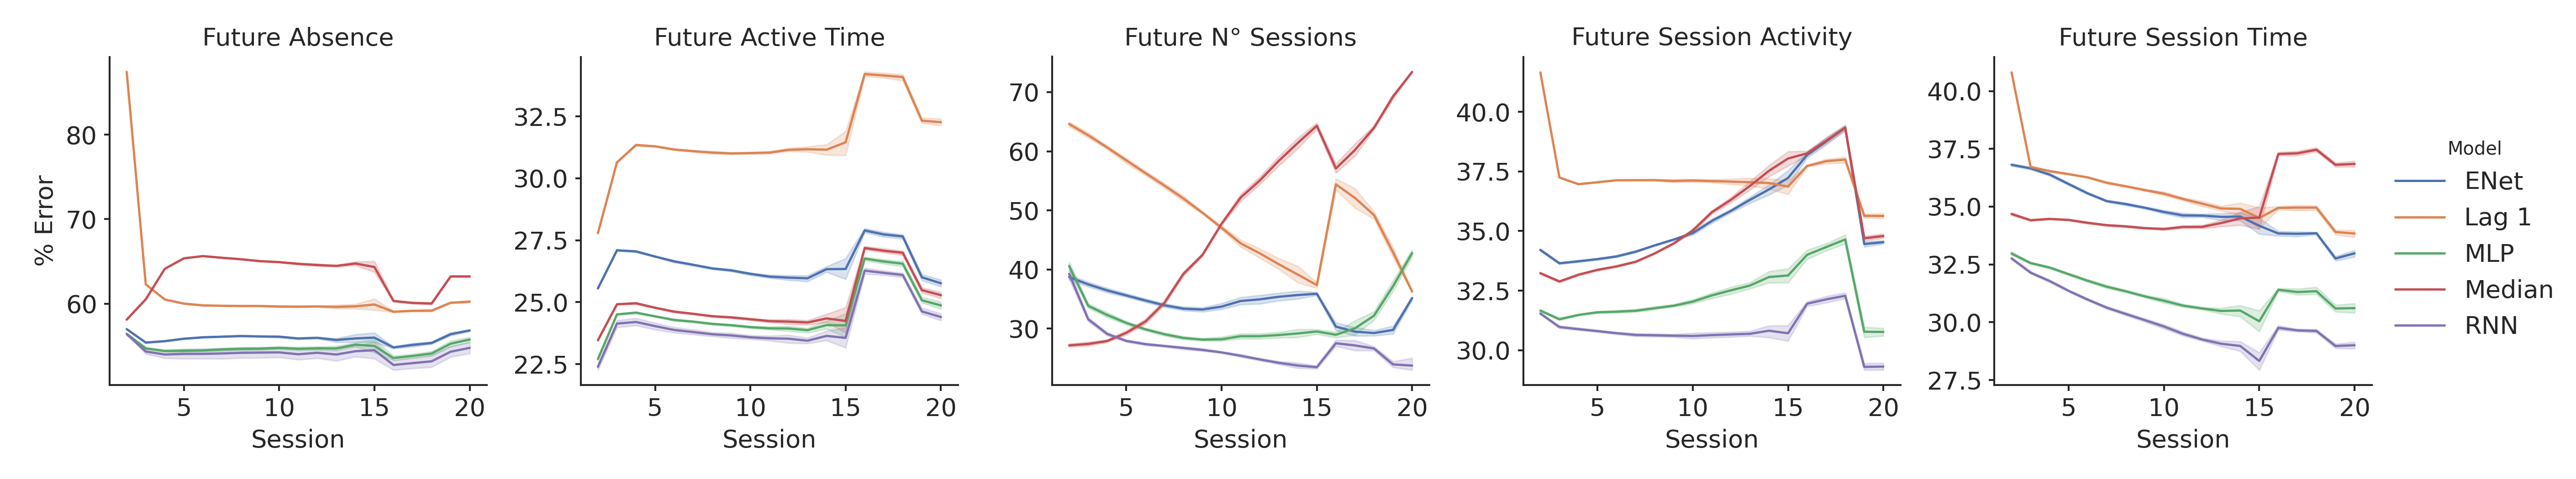
\includegraphics[width=\textwidth]{images/chapter_3/models_comparison_collapsed_game_32.png}
\caption[\textbf{Model comparison collapsing over game context}]{ Overall, our approach (RNN) outperforms all the competing approaches at every time horizon. Each column represent the perfromance of the considered models on a specific target. Solid lines indicate the expected \% error over time for a specific combination of target and model. Dashed areas indicate the standard error of the mean.}
\label{model_comp_coll_game_32}
\end{figure}
Similar conclusions can be drawn from inspecting the perfromance over the game-context dimension, Figure \ref{model_comp_coll_time_32}, where the RNN achieved the lowest error rate in almost every game context-target combination. In the few occasions in which this was not the case the perfromance was at least comparable with that of the MLP architecture (although always better when looking at the expected performance).
\begin{figure}[h]
\centering
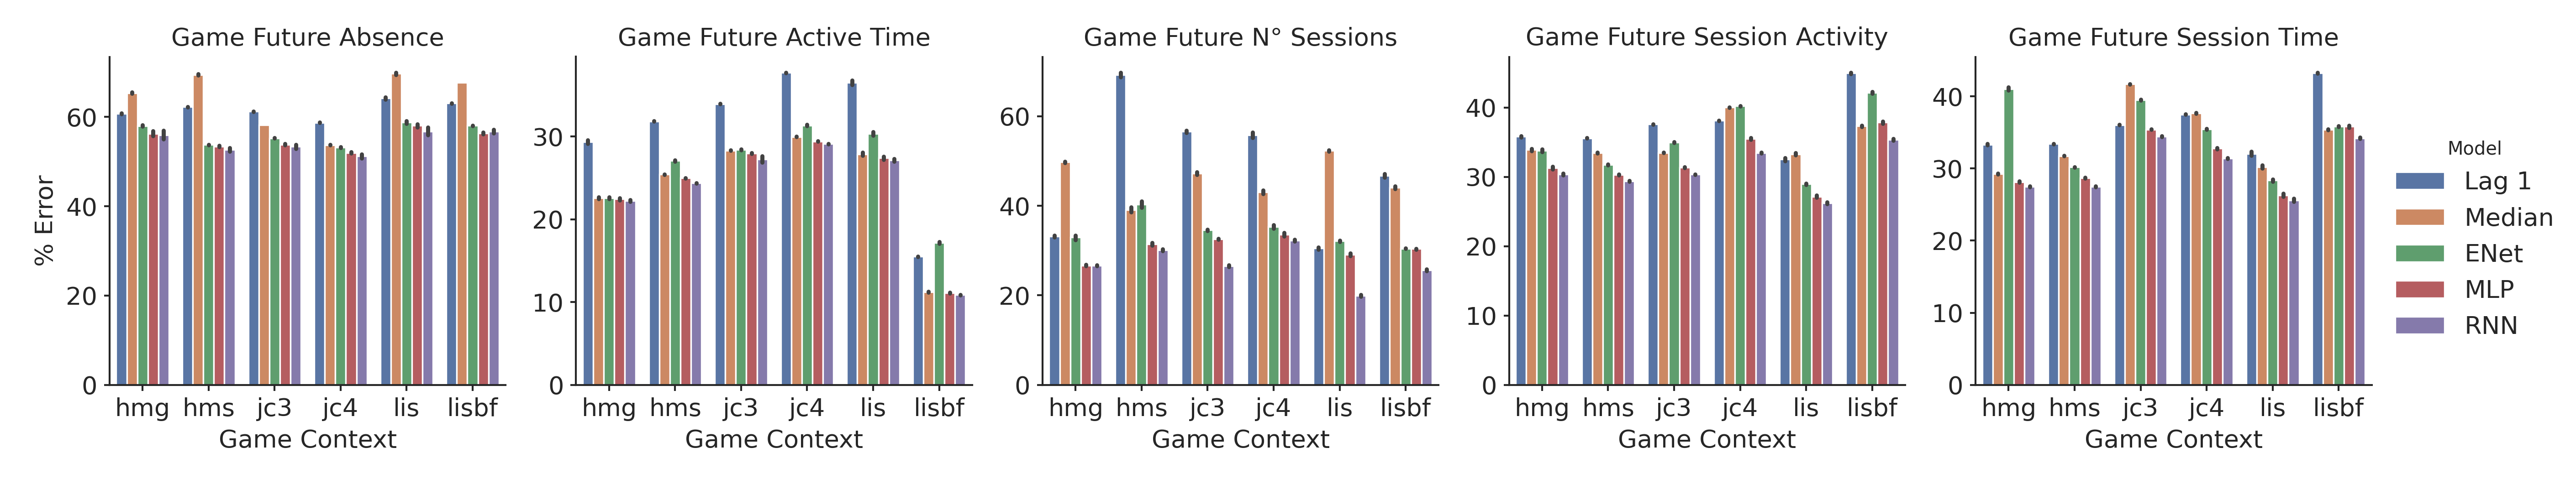
\includegraphics[width=\textwidth]{images/chapter_3/models_comparison_collapsed_time_32.png}
\caption[\textbf{Model comparison collapsing over time}]{ Overall, our approach (RNN) outperforms all the competing approaches in most of the target-game context combinations. Each column represent the perfromance of the considered models on a specific target. Bars indicate the expected \% error for a specific combination of game context, target and model. Black vertical lines indicate the standard error of the mean.}
\label{model_comp_coll_time_32} 
\end{figure}
These results remain almost unchanged even wen considering the interaction between game context and time (see Figure \ref{model_comp_non_coll_32}).
\begin{figure}[h]
\centering
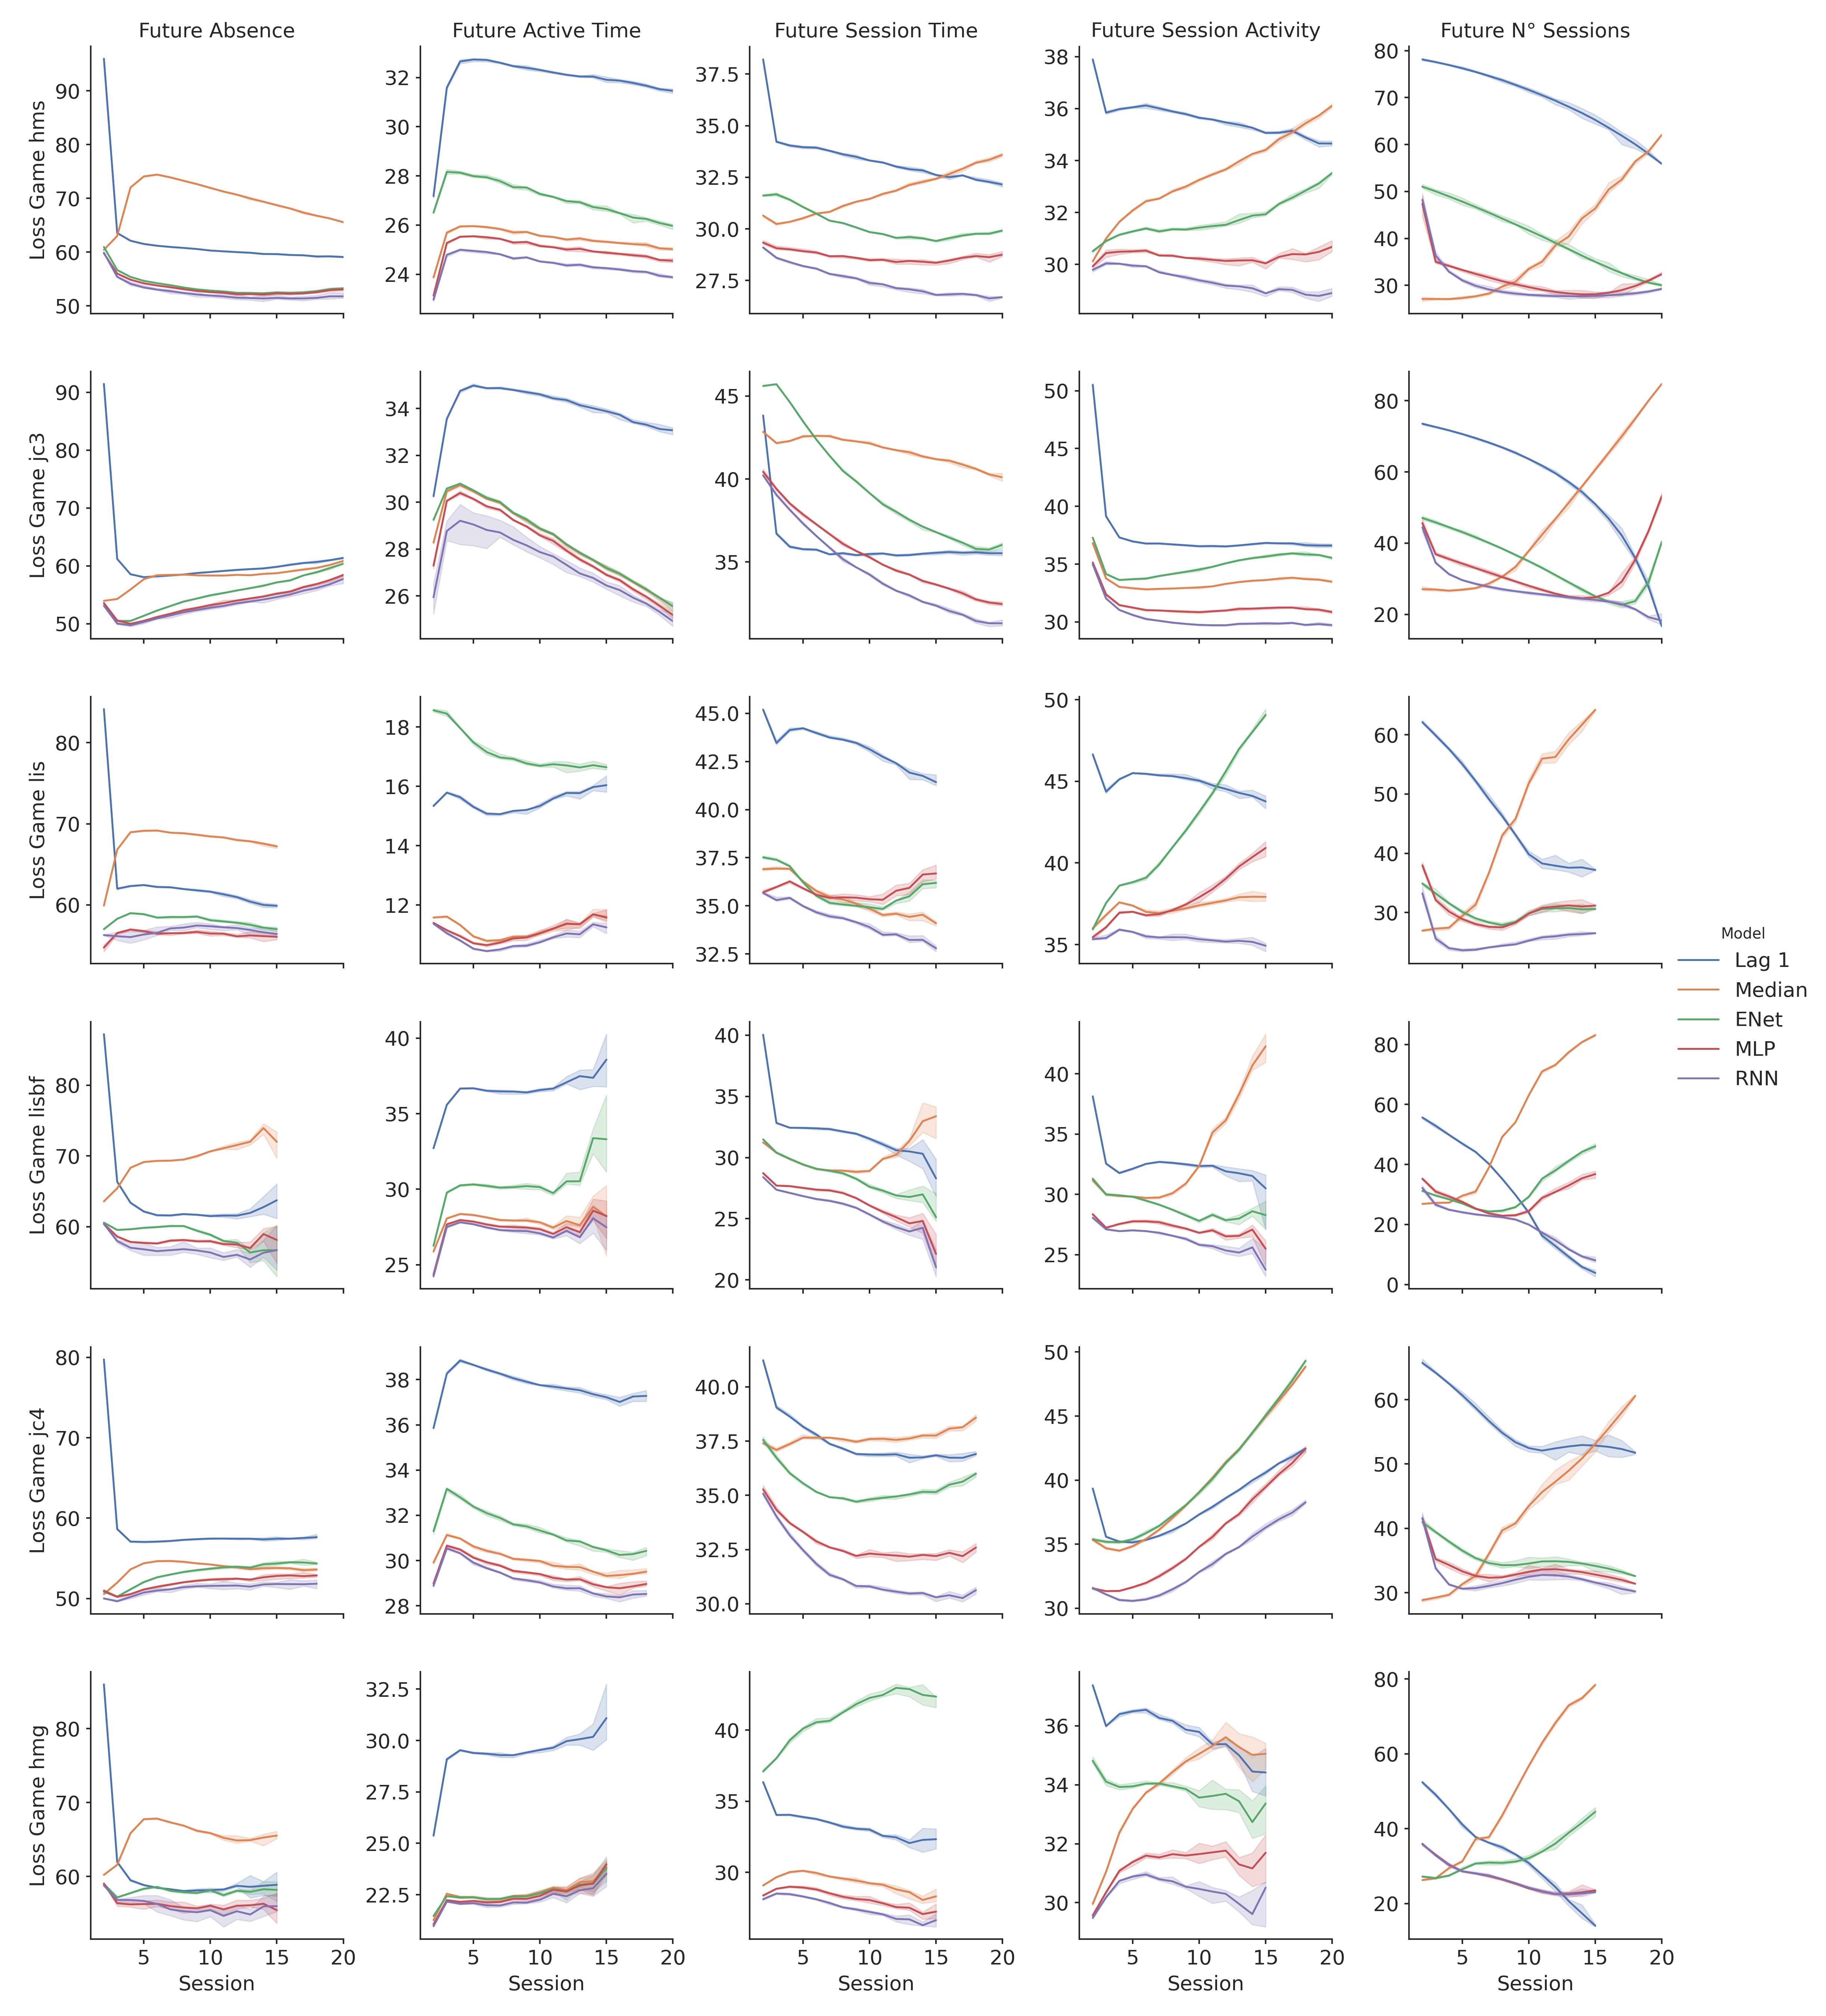
\includegraphics[height=0.5\textheight,keepaspectratio]{images/chapter_3/models_comparison_non_collapsed_32.png}
\caption[\textbf{Model comparison without collapsing}]{ Overall, our approach (RNN) outperforms all the competing approaches in most of the target-game context combinations and temporal horizons. Each column represents the perfromance of the considered models on a specific target while each row reports the perfromance on a specific game context. Solid lines indicate the expected \% error over time for a specific combination of target and model. Dashed areas indicate the standard error of the mean.}
\label{model_comp_non_coll_32} 
\end{figure}
At the level of global performance the RNN model markedly outperformed all competing approaches as clearly shown in Figure \ref{model_comp_coll_32}. This can be also seen in the results of the regression (see Table \ref{collapsed_lmm_32}) and  \textit{post hoc} analysis (see Table \ref{collapsed_post_hoc_32}). From the \textit{post hoc} analysis we can also observe how all the pairwise hypotheses presented in paragraph \ref{tuning_comparison_2} are confirmed. Here model performance is given by the sum of all the losses produced by the five targets and therefore provides a general indicator of model fit where lower values indicate a better performance overall.
\begin{figure}[h]
\centering
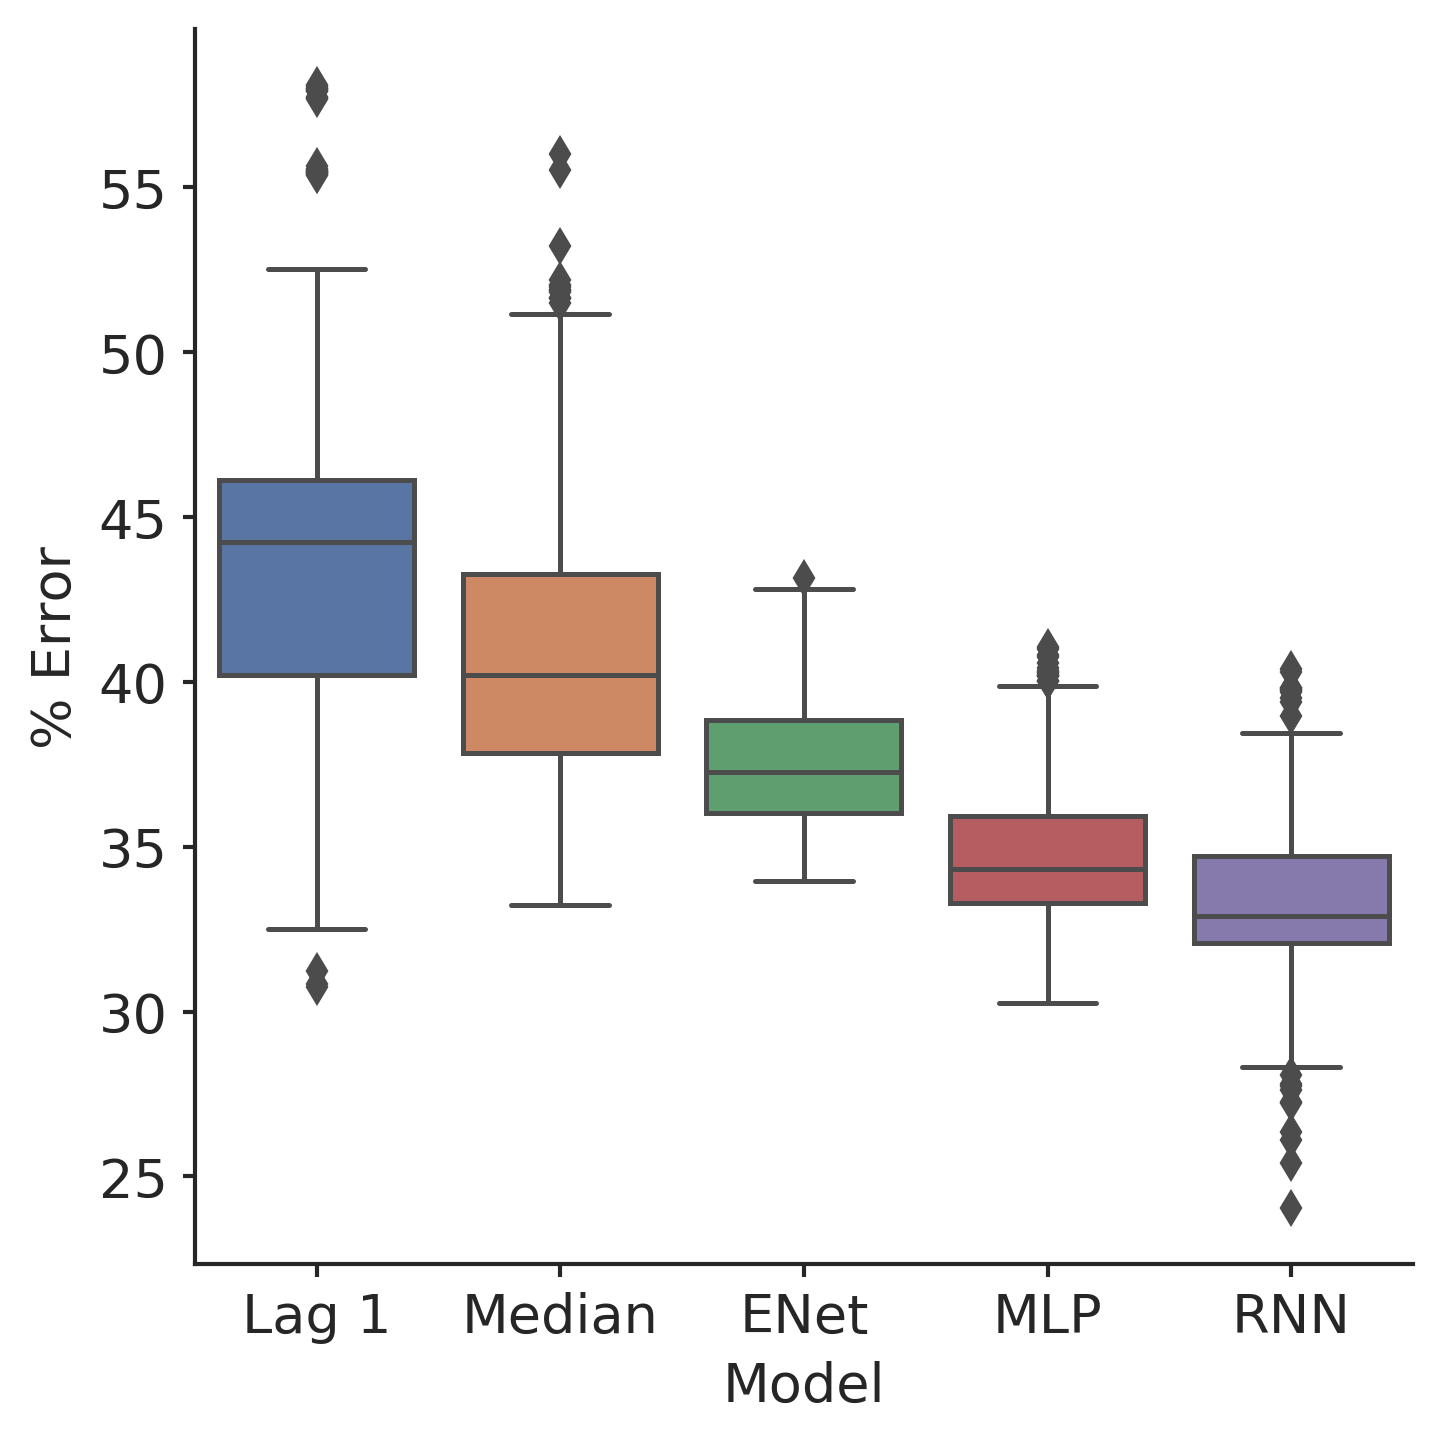
\includegraphics[width=.5\columnwidth]{images/chapter_3/performance_collapsed_32.png}
\caption[\textbf{Aggregated comparison of model performance}]{ Overall, our approach (RNN) outperforms all the competing approaches. Box-plots show the 10-fold cross-validation performance expressed as the total percentage of error (i.e. SMAPE) of each model over the five targets.}
\label{model_comp_coll_32} 
\end{figure}
\begin{table}[h]
\centering
\caption{Results of LMM on Collapsed Targets (Sum)}
\label{collapsed_target_lmm}
\resizebox{0.5\textwidth}{!}{
\begin{tabular}{ccccc}
\hline
\textbf{Model}           & \textbf{$\beta$} & \textbf{Z} & \textbf{p} & \textbf{95\% C.I.} \\ \hline
\multicolumn{5}{c}{\textbf{Collapsed Targets (Sum)}}                                                 \\ \hline
\textbf{Intercept (RNN)} & 33.129                & 41.799     & \textless .01   & 31.575 - 34.682      \\
\textbf{Lag 1}           & 10.010                 & 80.023     & \textless .01   & 9.765 - 10.255        \\
\textbf{Median}          & 7.482                 & 59.813     & \textless .01   & 7.237 - 7.727        \\
\textbf{ENet}            & 4.189                 & 33.491     & \textless .01   & 3.944 - 4.435        \\
\textbf{MLP}             & 1.411                 & 11.280     & \textless .01   & 1.166 - 1.656        \\ \hline
\end{tabular}
}
\end{table}
\begin{table}[h]
\centering
\caption{LMM Post-Hoc on Collapsed Targets (Sum)}
\label{collapsed_target_lmm_post_hoc}
\begin{tabular}{ccccc}
\hline
\textbf{Contrast}           & \textbf{$\beta_1$ - $\beta_2$} & \textbf{Z} & \textbf{p} & \textbf{95\% C.I.} \\ \hline
\multicolumn{5}{c}{\textbf{Collapsed Targets (Sum)}}                                                 \\ \hline
\textbf{Lag 1 - Median} & 2.528                & 20.210     & \textless .01   & 2.283 - 2.773      \\
\textbf{Median - ENet}          & 3.292                 & 26.322     & \textless .01   & 3.048 - 3.538        \\
\textbf{ENet - MLP}          & 2.778                 & 22.211     & \textless .01   & 2.533 - 3.024        \\ \hline
\end{tabular}
\end{table}
The superiority of the RNN model can still be observed when comparing the models on each target separately. However, the size of the effect varies depending on the target (see Table \ref{exploded_lmm_32}). The same trend is also present in the \textit{post hoc} analysis (see Table \ref{exploded_post_hoc_32}) where we observe only a partial confirmation of the pairwise hypotheses. The ENet model is outperformed by the Median baseline for three targets, namely Future Active Time, Session Time and Session Activity. All the coefficients in the regression analyses and the differences in the \textit{post hoc} analyses are non-standardized and can be interpreted as absolute changes in percentage error (i.e. SMAPE). In order to make these values more easily interpretable, we can use the information Table \ref{game_description_32}. For example, knowing that the median Session Time for the jc3 object is 162 minutes we can derive that when the RNN model achieves a SMAPE of 30\% in predicting Future Session Time, this equates on average to an absolute error of $1.62 \times 30 \sim 48$ minutes. All the p-values in the \textit{post hoc} analyses are Bonferroni corrected for multiple comparisons. The results of the statistical analyses suggest positive additive effects of non-linearity and recurrency on model performance both at the level of global and target-specific performance. This effect is more pronounced for certain targets (e.g. Future Session Time, Future N° Sessions) than for others (e.g. Future Absence, Future Active Time). Moreover, looking at Figure \ref{model_comp_exp_32} it appears that RNN improved on MLP (i.e. the second best model) using roughly half the parameters and per-epoch computation time. 
\begin{table}[h]
\centering
\caption{Results of LMM on Non-Collapsed Targets}
\label{exploded_target_lmm}
\begin{tabular}{ccccc}
\hline
\textbf{Model}  & \textbf{$\beta$} & \textbf{Z} & \textbf{p} & \textbf{95\% C.I.}                  \\ \hline
\multicolumn{5}{c}{\textbf{Future Absence}}                                                                         \\ \hline
\textbf{Intercept (RNN)} & 54.46                & 144.316     & \textless .01   & 53.72 - 55.20                     \\
\textbf{Lag 1}           & 7.40                & 40.509     & \textless .01   & 7.04 - 7.76                     \\
\textbf{Median}          & 9.47                & 51.814     & \textless .01   & 9.11 - 9.83                     \\
\textbf{ENet}            & 1.71                & 9.353     & \textless .01   & 1.35 - 2.06                     \\
\textbf{MLP}             & .53                & 2.915     & \textless .01   & .175 - .891                       \\ \hline
\multicolumn{5}{c}{\textbf{Future Active Time}}                                                                     \\ \hline
\textbf{Intercept (RNN)} & 23.36                & 20.019      & \textless .01  & 21.78 - 24.93                     \\
\textbf{Lag 1}           & 7.32               & 119.028    & \textless .01  & 7.2 - 7.44                     \\
\textbf{Median}          & .77                & 12.515     & \textless .01  & .649 - .891                     \\
\textbf{ENet}            & 2.55                & 41.551     & \textless .01  & 2.43 - 2.67                     \\
\textbf{MLP}             & .41                & 6.739      & \textless .01  & .294 - .535                     \\ \hline
\multicolumn{5}{c}{\textbf{Future Session Time}}                                                                     \\ \hline
\textbf{Intercept (RNN)} & 30.02                & 63.663     & \textless .01  & 29.1 - 30.95                     \\
\textbf{Lag 1}            & 5.62                & 49.158     & \textless .01  & 5.39 - 5.83                     \\
\textbf{Median}          & 4.45                & 38.957     & \textless .01  & 4.23 - 4.67                     \\
\textbf{ENet}            & 4.81                & 42.098     & \textless .01  & 4.59 - 5.03                     \\
\textbf{MLP}             & 1.08                & 9.529      & \textless .01  & .86 - 1.31                     \\ \hline
\multicolumn{5}{c}{\textbf{Future Session Activity}}                                                                 \\ \hline
\textbf{Intercept (RNN)} & 31.04                & 70.241     & \textless .01  & \multicolumn{1}{l}{30.17 - 31.9} \\
\textbf{Lag 1}            & 6.52                & 61.025     & \textless .01  & \multicolumn{1}{l}{6.31 - 6.73} \\
\textbf{Median}          & 4.37                & 40.879     & \textless .01  & \multicolumn{1}{l}{4.16 - 4.58} \\
\textbf{ENet}            & 4.42                & 41.319     & \textless .01  & \multicolumn{1}{l}{4.21 - 4.63} \\
\textbf{MLP}             & 1.36                & 12.762     & \textless .01  & \multicolumn{1}{l}{1.15 - 1.57} \\ \hline
\multicolumn{5}{c}{\textbf{Future N° Sessions}}                                                                      \\ \hline
\textbf{Intercept (RNN)} & 26.77                & 7.445     & \textless .01  & 19.72 - 33.81                     \\
\textbf{Lag 1}            & 23.17                & 44.430     & \textless .01  & 22.15 - 24.19                     \\
\textbf{Median}          &  18.34              & 35.166     & \textless .01  & 17.31 - 19.36                     \\
\textbf{ENet}            & 7.44                & 14.277     & \textless .01  & 6.42 - 8.46                     \\
\textbf{MLP}             & 3.65                & 7.005      & \textless .01  & 2.63 - 4.67                       \\ \hline
\end{tabular}
\end{table}
\begin{table}[h]
\centering
\caption{LMM Post-Hoc on Non-Collapsed Targets}
\label{exploded_target_lmm_post_hoc}
\begin{tabular}{ccccc}
\hline
\textbf{Contrast}  & \textbf{$\beta_1$-$\beta_2$} & \textbf{Z} & \textbf{p} & \textbf{95\% C.I.}                  \\ \hline
\multicolumn{5}{c}{\textbf{Future Absence}}                                                                         \\ \hline
\textbf{Lag 1 - Median} & -2.06                & -11.305     & \textless .01   & -2.42 - -1.70                     \\
\textbf{Median - ENet}           & 7.76                & 42.461     & \textless .01   & 7.40 - 8.12                     \\
\textbf{ENet - MLP}          & 1.17                & 6.438     & \textless .01   & .81 - 1.535                    \\ \hline
\multicolumn{5}{c}{\textbf{Future Active Time}}                                                                     \\ \hline
\textbf{Lag 1 - Median} & 6.55                & 106.513      & \textless .01  & 6.433 - 6.67                     \\
\textbf{Median - ENet}           & -1.78                & -29.037    & \textless .01  & -1.9 - -1.66                     \\
\textbf{ENet - MLP}          & 2.14                & 34.812     & \textless .01  & 2.02 - 2.26                     \\\hline
\multicolumn{5}{c}{\textbf{Future Session Time}}                                                                     \\ \hline
\textbf{Lag 1 - Median} & 1.16                & 10.201     & \textless .01  & .94 - 1.39                     \\
\textbf{Median - ENet}            & -.35                & -3.141     & \textless .01  & -.58 - -.13                     \\
\textbf{ENet - MLP}          & 3.72                & 32.579     & \textless .01  & 3.5 - 3.95                     \\ \hline
\multicolumn{5}{c}{\textbf{Future Session Activity}}                                                                 \\ \hline
\textbf{Lag 1 - Median} & 2.15                & 20.146     & \textless .01  & \multicolumn{1}{l}{1.94 - 2.36} \\
\textbf{Median - ENet}            & -.04                & -.441     &  1.  & \multicolumn{1}{l}{-.257 - .163} \\
\textbf{ENet - MLP}          & 3.05                & 28.558     & \textless .01  & \multicolumn{1}{l}{2.84 - 3.26} \\ \hline
\multicolumn{5}{c}{\textbf{Future N° Sessions}}                                                                      \\ \hline
\textbf{Lag 1 - Median} & 4.83                & 9.264     & \textless .01  & 3.8 - 5.85                     \\
\textbf{Median - ENet}            & 10.89                & 20.889     & \textless .01  & 9.87 - 11.91                     \\
\textbf{ENet - MLP}          & 3.79                & 7.272     & \textless .01  & 2.77 - 4.81                     \\\hline
\end{tabular}
\end{table}
\begin{figure*}[h]
\centering
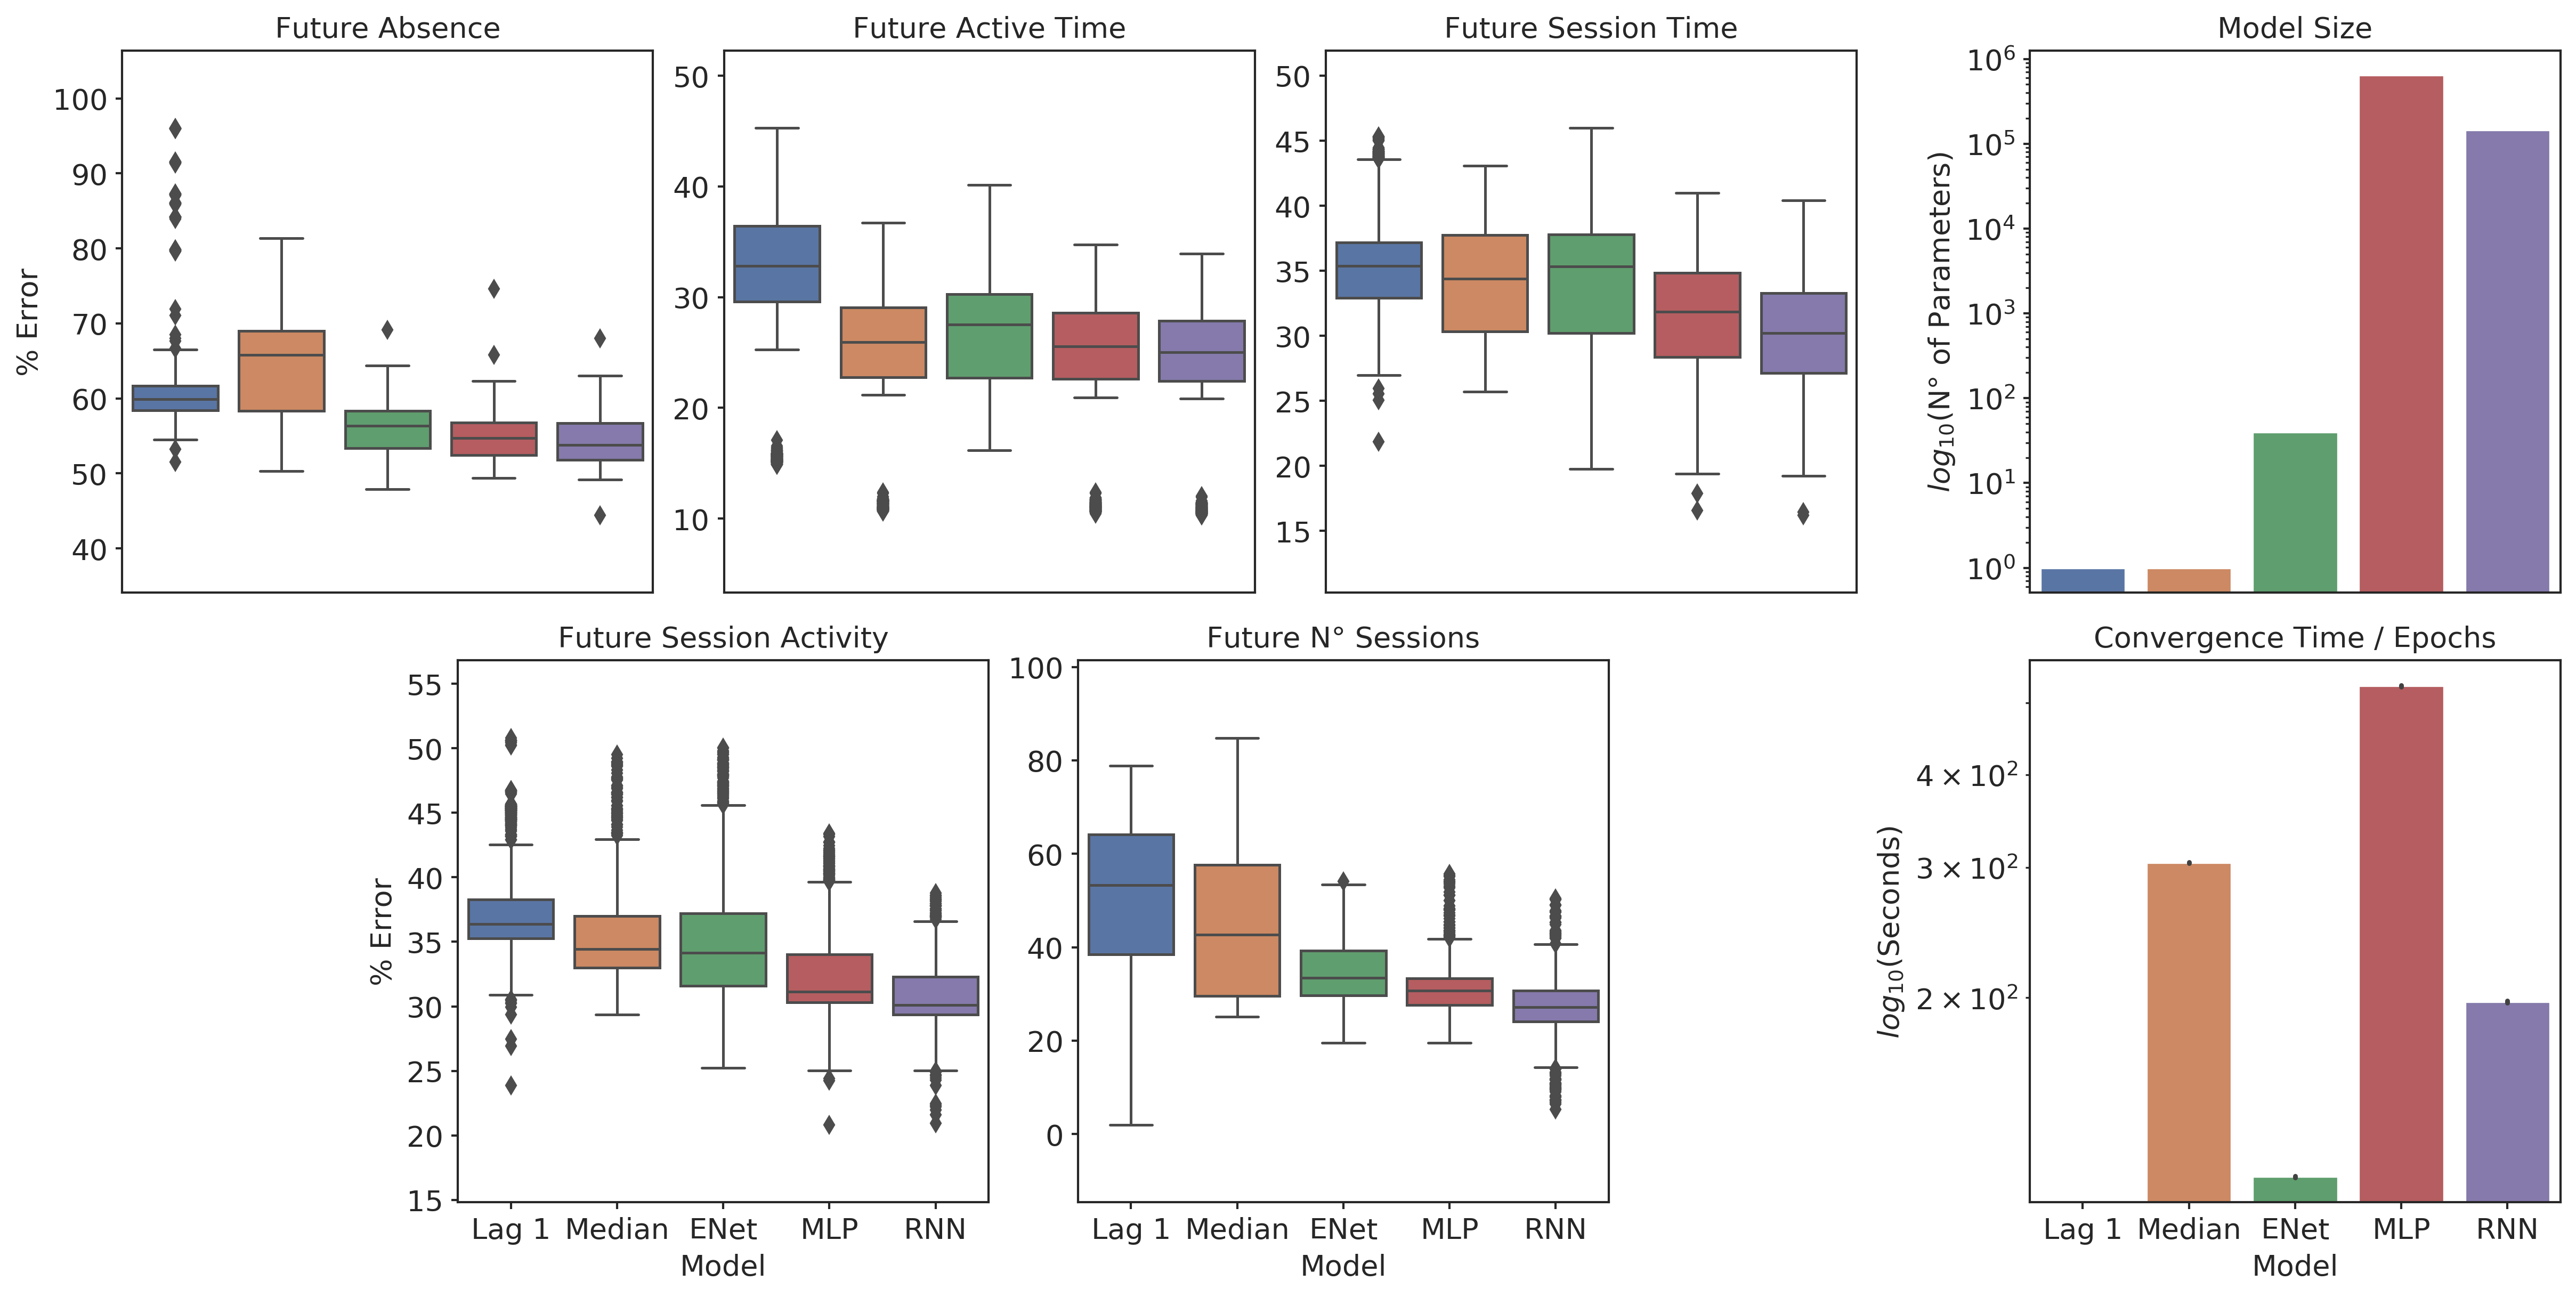
\includegraphics[width=.8\textwidth]{images/chapter_3/performance_exploded_32.png}
\caption[\textbf{Dis-aggregated comparison of models' performance}]{Our approach (RNN) outperformed all competing ones on each target. It consistently used fewer parameters and had shorter computation time than the second best performing model. Box-plots show the 10-fold cross-validation performance expressed as percentage of error (i.e. SMAPE) of each model for the five targets. The bar-plot on the top row indicates the number of free parameters for each model while the bar plot on the bottom row shows the average time for each training epoch. Both bar-plots are $log_{10}$ scaled.}
\label{model_comp_exp_32} 
\end{figure*}

\subsection{Model Criticism}
\label{model_criticims_2}
Similarly to what presented in section \ref{results_1} we were able to observe different level of perfromance for the baseline models in different game contexts, suggesting once again an heterogeneity in the level of challenge for the predictive task. A similar level of heterogeneity was also found among the considered behavioural targets (e.g. Future Absence appeared to be a much harder target to predict than Future N° of Sessions) and temporal horizons (e.g. predictions made at an early or late stage showed to be more or less challenging depending on the considered target, game context and model architecture). By looking at the performance of the various parametric models we were able to replicate our initial findings, suggesting the importance of modelling non-linear dynamics when predicting measures of future behavioural intensity. When a model provided better perfromance than a competing one it did so among all the considered game contexts and behavioural targets, again confirming that the adopted global multi-task learning approach did not cause any degradation in predictive accuracy. In summary, improving the BM model and modifying its architecture in order to better incorporate the theoretical constrains outlined in chapter \ref{chapter_theory_modelling} did not substantially change any of the findings reported in the first iteration of the model building process. That said, despite the RNN architecture was now able to generate representations compatible with the computational frameworks presented by McClure et al. \cite{mcclure2003computational} and Zhang et al. \cite{zhang2009neural} it was still not taking into account factors that might be relevant for reliably estimating the level of attributed incentive salience. Indeed, as we mentioned in chapter \ref{chapter_lit_review}, we know that this type of latent state, and its associated dynamics, are modulated by the internal condition of the individual \cite{zhang2009neural}, by the characteristics of the rewarding object (a specific videogame in this case) with which the individual is interacting and by the environment in which the interaction is occurring \cite{palminteri2015contextual}. These factors, were only partially and indirectly captured by the RNN architecture as they require more granular information (i.e. in-game and environmental information) and with a higher temporal resolution (i.e. within rather than between game sessions). As a consequence we can see how the RNN architecture, despite outperforming competing ones, still achieves a relatively high error rate in predicting some of the considered behavioural targets (e.g. future Absence). A possible solution in this case would be to incorporate information about the environment in which the observed behaviour occurred (e.g. time and location of a specific game session) and about the characteristics of the rewarding objects (i.e. the so called videogame structural characteristics that we mentioned in chapter \ref{chapter_lit_review}). As well as improving the predictive performance of the model, these new type of information should also increase the quality of the generated representation and consequently allow for a better approximation of the level of attributed incentive salience. The next iteration of the model building process will aim at modifying the RNN architecture in order to incorporate the type of environmental and game-specific information that we just mentioned.

\section{Dynamic Prediction of Future Behavioural Intensity with Environmental and Game Covariates}
\label{model_architecture_3}
\lorem

\subsection{Model Design}
\label{model_design_3}
\lorem
\begin{figure}[ht]
\begin{center}
\begin{adjustbox}{width=0.7\textwidth}
    \tikzset{every picture/.style={line width=0.75pt}} %set default line width to 0.75pt        
    
    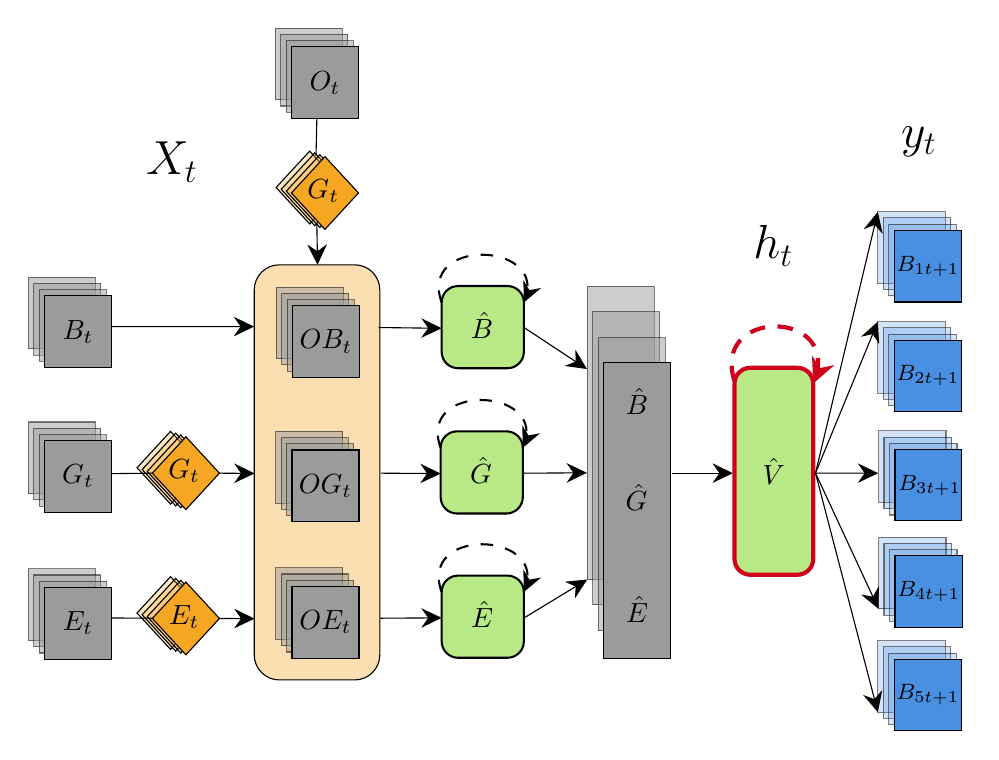
\begin{tikzpicture}[x=0.75pt,y=0.75pt,yscale=-1,xscale=1]
    %uncomment if require: \path (0,411); %set diagram left start at 0, and has height of 411
    
    %Rounded Rect [id:dp15650356150345013] 
    \draw  [fill={rgb, 255:red, 245; green, 166; blue, 35 }  ,fill opacity=0.36 ] (219.9,142.15) .. controls (219.9,135.47) and (225.32,130.05) .. (232,130.05) -- (268.3,130.05) .. controls (274.98,130.05) and (280.4,135.47) .. (280.4,142.15) -- (280.4,317.95) .. controls (280.4,324.63) and (274.98,330.05) .. (268.3,330.05) -- (232,330.05) .. controls (225.32,330.05) and (219.9,324.63) .. (219.9,317.95) -- cycle ;
    %Straight Lines [id:da409284418173784] 
    \draw    (250.06,109.76) -- (250.35,127.05) ;
    \draw [shift={(250.4,130.05)}, rotate = 269.03] [fill={rgb, 255:red, 0; green, 0; blue, 0 }  ][line width=0.08]  [draw opacity=0] (9.82,-4.72) -- (0,0) -- (9.82,4.72) -- (6.52,0) -- cycle    ;
    %Shape: Rectangle [id:dp7034345660290355] 
    \draw  [color={rgb, 255:red, 0; green, 0; blue, 0 }  ,draw opacity=0.5 ][fill={rgb, 255:red, 155; green, 155; blue, 155 }  ,fill opacity=0.5 ] (111.01,276.53) -- (143.26,276.53) -- (143.26,311.05) -- (111.01,311.05) -- cycle ;
    %Shape: Rectangle [id:dp22118233628007533] 
    \draw  [color={rgb, 255:red, 0; green, 0; blue, 0 }  ,draw opacity=0.5 ][fill={rgb, 255:red, 155; green, 155; blue, 155 }  ,fill opacity=0.5 ] (113.63,279.51) -- (145.88,279.51) -- (145.88,314.03) -- (113.63,314.03) -- cycle ;
    %Shape: Rectangle [id:dp24867768000931467] 
    \draw  [color={rgb, 255:red, 0; green, 0; blue, 0 }  ,draw opacity=0.5 ][fill={rgb, 255:red, 155; green, 155; blue, 155 }  ,fill opacity=0.5 ] (116.27,282.56) -- (148.53,282.56) -- (148.53,317.08) -- (116.27,317.08) -- cycle ;
    %Shape: Rectangle [id:dp124905579804508] 
    \draw  [fill={rgb, 255:red, 155; green, 155; blue, 155 }  ,fill opacity=1 ] (118.86,285.5) -- (151.11,285.5) -- (151.11,320.02) -- (118.86,320.02) -- cycle ;
    %Straight Lines [id:da8537240673366849] 
    \draw    (250.06,59.86) -- (249.67,77.43) ;
    %Rounded Rect [id:dp9724403504665806] 
    \draw  [color={rgb, 255:red, 208; green, 2; blue, 27 }  ,draw opacity=1 ][fill={rgb, 255:red, 184; green, 233; blue, 134 }  ,fill opacity=1 ][line width=1.5]  (451.3,187.25) .. controls (451.3,183.06) and (454.7,179.67) .. (458.88,179.67) -- (481.62,179.67) .. controls (485.81,179.67) and (489.2,183.06) .. (489.2,187.25) -- (489.2,271.79) .. controls (489.2,275.97) and (485.81,279.37) .. (481.62,279.37) -- (458.88,279.37) .. controls (454.7,279.37) and (451.3,275.97) .. (451.3,271.79) -- cycle ;
    %Curve Lines [id:da6973720397061056] 
    \draw [color={rgb, 255:red, 208; green, 2; blue, 27 }  ,draw opacity=1 ][line width=1.5]  [dash pattern={on 5.63pt off 4.5pt}]  (451.3,186.02) .. controls (439.95,151.4) and (500.2,151.33) .. (490.53,183.61) ;
    \draw [shift={(489.2,187.25)}, rotate = 293.32] [fill={rgb, 255:red, 208; green, 2; blue, 27 }  ,fill opacity=1 ][line width=0.08]  [draw opacity=0] (12.23,-5.88) -- (0,0) -- (12.23,5.88) -- (8.12,0) -- cycle    ;
    %Shape: Rectangle [id:dp1958055080757597] 
    \draw  [color={rgb, 255:red, 0; green, 0; blue, 0 }  ,draw opacity=0.5 ][fill={rgb, 255:red, 74; green, 144; blue, 226 }  ,fill opacity=0.25 ] (520.36,157.39) -- (552.87,157.39) -- (552.87,191.9) -- (520.36,191.9) -- cycle ;
    %Shape: Rectangle [id:dp20825701586292622] 
    \draw  [color={rgb, 255:red, 0; green, 0; blue, 0 }  ,draw opacity=0.5 ][fill={rgb, 255:red, 74; green, 144; blue, 226 }  ,fill opacity=0.25 ] (523,160.37) -- (555.51,160.37) -- (555.51,194.88) -- (523,194.88) -- cycle ;
    %Shape: Rectangle [id:dp6709034910590727] 
    \draw  [color={rgb, 255:red, 0; green, 0; blue, 0 }  ,draw opacity=0.5 ][fill={rgb, 255:red, 74; green, 144; blue, 226 }  ,fill opacity=0.25 ] (525.67,163.42) -- (558.17,163.42) -- (558.17,197.93) -- (525.67,197.93) -- cycle ;
    %Shape: Rectangle [id:dp943426610209301] 
    \draw  [fill={rgb, 255:red, 74; green, 144; blue, 226 }  ,fill opacity=1 ] (528.28,166.36) -- (560.78,166.36) -- (560.78,200.87) -- (528.28,200.87) -- cycle ;
    %Shape: Rectangle [id:dp9270730461824767] 
    \draw  [color={rgb, 255:red, 0; green, 0; blue, 0 }  ,draw opacity=0.5 ][fill={rgb, 255:red, 74; green, 144; blue, 226 }  ,fill opacity=0.25 ] (520.69,210.06) -- (553.2,210.06) -- (553.2,244.56) -- (520.69,244.56) -- cycle ;
    %Shape: Rectangle [id:dp9671567967621458] 
    \draw  [color={rgb, 255:red, 0; green, 0; blue, 0 }  ,draw opacity=0.5 ][fill={rgb, 255:red, 74; green, 144; blue, 226 }  ,fill opacity=0.25 ] (523.33,213.04) -- (555.84,213.04) -- (555.84,247.54) -- (523.33,247.54) -- cycle ;
    %Shape: Rectangle [id:dp6567850092606636] 
    \draw  [color={rgb, 255:red, 0; green, 0; blue, 0 }  ,draw opacity=0.5 ][fill={rgb, 255:red, 74; green, 144; blue, 226 }  ,fill opacity=0.25 ] (526,216.09) -- (558.5,216.09) -- (558.5,250.6) -- (526,250.6) -- cycle ;
    %Shape: Rectangle [id:dp9307909660529495] 
    \draw  [fill={rgb, 255:red, 74; green, 144; blue, 226 }  ,fill opacity=1 ] (528.62,219.02) -- (560.84,219.02) -- (560.84,253.22) -- (528.62,253.22) -- cycle ;
    %Shape: Rectangle [id:dp2956426995252315] 
    \draw  [color={rgb, 255:red, 0; green, 0; blue, 0 }  ,draw opacity=0.5 ][fill={rgb, 255:red, 74; green, 144; blue, 226 }  ,fill opacity=0.25 ] (520.36,311.11) -- (552.87,311.11) -- (552.87,345.62) -- (520.36,345.62) -- cycle ;
    %Shape: Rectangle [id:dp9676718309145981] 
    \draw  [color={rgb, 255:red, 0; green, 0; blue, 0 }  ,draw opacity=0.5 ][fill={rgb, 255:red, 74; green, 144; blue, 226 }  ,fill opacity=0.25 ] (523,314.09) -- (555.51,314.09) -- (555.51,348.6) -- (523,348.6) -- cycle ;
    %Shape: Rectangle [id:dp3802447939611997] 
    \draw  [color={rgb, 255:red, 0; green, 0; blue, 0 }  ,draw opacity=0.5 ][fill={rgb, 255:red, 74; green, 144; blue, 226 }  ,fill opacity=0.25 ] (525.67,317.14) -- (558.17,317.14) -- (558.17,351.65) -- (525.67,351.65) -- cycle ;
    %Shape: Rectangle [id:dp2655409211543931] 
    \draw  [fill={rgb, 255:red, 74; green, 144; blue, 226 }  ,fill opacity=1 ] (528.28,320.08) -- (560.78,320.08) -- (560.78,354.59) -- (528.28,354.59) -- cycle ;
    %Shape: Rectangle [id:dp4040153422296009] 
    \draw  [color={rgb, 255:red, 0; green, 0; blue, 0 }  ,draw opacity=0.5 ][fill={rgb, 255:red, 74; green, 144; blue, 226 }  ,fill opacity=0.25 ] (520.69,261.32) -- (553.2,261.32) -- (553.2,295.83) -- (520.69,295.83) -- cycle ;
    %Shape: Rectangle [id:dp7066102537923638] 
    \draw  [color={rgb, 255:red, 0; green, 0; blue, 0 }  ,draw opacity=0.5 ][fill={rgb, 255:red, 74; green, 144; blue, 226 }  ,fill opacity=0.25 ] (523.33,264.3) -- (555.84,264.3) -- (555.84,298.81) -- (523.33,298.81) -- cycle ;
    %Shape: Rectangle [id:dp46050637304135866] 
    \draw  [color={rgb, 255:red, 0; green, 0; blue, 0 }  ,draw opacity=0.5 ][fill={rgb, 255:red, 74; green, 144; blue, 226 }  ,fill opacity=0.25 ] (526,267.35) -- (558.5,267.35) -- (558.5,301.86) -- (526,301.86) -- cycle ;
    %Shape: Rectangle [id:dp2033829273595421] 
    \draw  [fill={rgb, 255:red, 74; green, 144; blue, 226 }  ,fill opacity=1 ] (528.61,270.29) -- (561.11,270.29) -- (561.11,304.8) -- (528.61,304.8) -- cycle ;
    %Shape: Rectangle [id:dp19424752965877823] 
    \draw  [color={rgb, 255:red, 0; green, 0; blue, 0 }  ,draw opacity=0.5 ][fill={rgb, 255:red, 74; green, 144; blue, 226 }  ,fill opacity=0.25 ] (520.36,104.48) -- (552.87,104.48) -- (552.87,138.98) -- (520.36,138.98) -- cycle ;
    %Shape: Rectangle [id:dp6987771152166413] 
    \draw  [color={rgb, 255:red, 0; green, 0; blue, 0 }  ,draw opacity=0.5 ][fill={rgb, 255:red, 74; green, 144; blue, 226 }  ,fill opacity=0.25 ] (523,107.46) -- (555.51,107.46) -- (555.51,141.96) -- (523,141.96) -- cycle ;
    %Shape: Rectangle [id:dp12765942569283661] 
    \draw  [color={rgb, 255:red, 0; green, 0; blue, 0 }  ,draw opacity=0.5 ][fill={rgb, 255:red, 74; green, 144; blue, 226 }  ,fill opacity=0.25 ] (525.67,110.51) -- (558.17,110.51) -- (558.17,145.01) -- (525.67,145.01) -- cycle ;
    %Shape: Rectangle [id:dp16248810139444148] 
    \draw  [fill={rgb, 255:red, 74; green, 144; blue, 226 }  ,fill opacity=1 ] (528.28,113.44) -- (560.78,113.44) -- (560.78,147.95) -- (528.28,147.95) -- cycle ;
    %Shape: Rectangle [id:dp7988673729176894] 
    \draw  [color={rgb, 255:red, 0; green, 0; blue, 0 }  ,draw opacity=0.5 ][fill={rgb, 255:red, 155; green, 155; blue, 155 }  ,fill opacity=0.5 ] (111.01,205.77) -- (143.26,205.77) -- (143.26,240.29) -- (111.01,240.29) -- cycle ;
    %Shape: Rectangle [id:dp9623129937085917] 
    \draw  [color={rgb, 255:red, 0; green, 0; blue, 0 }  ,draw opacity=0.5 ][fill={rgb, 255:red, 155; green, 155; blue, 155 }  ,fill opacity=0.5 ] (113.63,208.75) -- (145.88,208.75) -- (145.88,243.27) -- (113.63,243.27) -- cycle ;
    %Shape: Rectangle [id:dp429379441325212] 
    \draw  [color={rgb, 255:red, 0; green, 0; blue, 0 }  ,draw opacity=0.5 ][fill={rgb, 255:red, 155; green, 155; blue, 155 }  ,fill opacity=0.5 ] (116.27,211.8) -- (148.53,211.8) -- (148.53,246.32) -- (116.27,246.32) -- cycle ;
    %Shape: Rectangle [id:dp9493890675957639] 
    \draw  [fill={rgb, 255:red, 155; green, 155; blue, 155 }  ,fill opacity=1 ] (118.86,214.74) -- (151.11,214.74) -- (151.11,249.26) -- (118.86,249.26) -- cycle ;
    %Straight Lines [id:da0399560958706785] 
    \draw [fill={rgb, 255:red, 155; green, 155; blue, 155 }  ,fill opacity=1 ]   (150.09,159.83) -- (216.85,159.8) ;
    \draw [shift={(219.85,159.8)}, rotate = 179.98] [fill={rgb, 255:red, 0; green, 0; blue, 0 }  ][line width=0.08]  [draw opacity=0] (9.82,-4.72) -- (0,0) -- (9.82,4.72) -- (6.52,0) -- cycle    ;
    %Shape: Rectangle [id:dp3393145890474042] 
    \draw  [color={rgb, 255:red, 0; green, 0; blue, 0 }  ,draw opacity=0.5 ][fill={rgb, 255:red, 155; green, 155; blue, 155 }  ,fill opacity=0.5 ] (111.01,136.06) -- (143.26,136.06) -- (143.26,170.57) -- (111.01,170.57) -- cycle ;
    %Shape: Rectangle [id:dp27631704382885136] 
    \draw  [color={rgb, 255:red, 0; green, 0; blue, 0 }  ,draw opacity=0.5 ][fill={rgb, 255:red, 155; green, 155; blue, 155 }  ,fill opacity=0.5 ] (113.63,139.04) -- (145.88,139.04) -- (145.88,173.55) -- (113.63,173.55) -- cycle ;
    %Shape: Rectangle [id:dp8553441662393909] 
    \draw  [color={rgb, 255:red, 0; green, 0; blue, 0 }  ,draw opacity=0.5 ][fill={rgb, 255:red, 155; green, 155; blue, 155 }  ,fill opacity=0.5 ] (116.27,142.09) -- (148.53,142.09) -- (148.53,176.61) -- (116.27,176.61) -- cycle ;
    %Shape: Rectangle [id:dp4571491350911555] 
    \draw  [fill={rgb, 255:red, 155; green, 155; blue, 155 }  ,fill opacity=1 ] (118.86,145.03) -- (151.11,145.03) -- (151.11,179.54) -- (118.86,179.54) -- cycle ;
    %Shape: Diamond [id:dp42134346339770745] 
    \draw  [fill={rgb, 255:red, 245; green, 166; blue, 35 }  ,fill opacity=0.25 ] (179.6,210.28) -- (195.77,227.81) -- (179.6,245.33) -- (163.43,227.81) -- cycle ;
    %Shape: Diamond [id:dp8160874162123375] 
    \draw  [fill={rgb, 255:red, 245; green, 166; blue, 35 }  ,fill opacity=0.25 ] (182.05,211.16) -- (198.22,228.68) -- (182.05,246.2) -- (165.89,228.68) -- cycle ;
    %Shape: Diamond [id:dp05986250472128074] 
    \draw  [fill={rgb, 255:red, 245; green, 166; blue, 35 }  ,fill opacity=0.25 ] (184.51,212.04) -- (200.68,229.56) -- (184.51,247.08) -- (168.34,229.56) -- cycle ;
    %Shape: Diamond [id:dp6831575900746938] 
    \draw  [fill={rgb, 255:red, 245; green, 166; blue, 35 }  ,fill opacity=1 ] (186.97,212.91) -- (203.13,230.43) -- (186.97,247.96) -- (170.8,230.43) -- cycle ;
    %Straight Lines [id:da3169233008507637] 
    \draw    (151.46,230.66) -- (170.8,230.43) ;
    %Shape: Diamond [id:dp08100159339963764] 
    \draw  [fill={rgb, 255:red, 245; green, 166; blue, 35 }  ,fill opacity=0.25 ] (179.6,280.28) -- (195.77,297.81) -- (179.6,315.33) -- (163.43,297.81) -- cycle ;
    %Shape: Diamond [id:dp6545409040088919] 
    \draw  [fill={rgb, 255:red, 245; green, 166; blue, 35 }  ,fill opacity=0.25 ] (182.05,281.16) -- (198.22,298.68) -- (182.05,316.2) -- (165.89,298.68) -- cycle ;
    %Shape: Diamond [id:dp22008618792927115] 
    \draw  [fill={rgb, 255:red, 245; green, 166; blue, 35 }  ,fill opacity=0.25 ] (184.51,282.04) -- (200.68,299.56) -- (184.51,317.08) -- (168.34,299.56) -- cycle ;
    %Shape: Diamond [id:dp6216162169932065] 
    \draw  [fill={rgb, 255:red, 245; green, 166; blue, 35 }  ,fill opacity=1 ] (186.97,282.91) -- (203.13,300.43) -- (186.97,317.96) -- (170.8,300.43) -- cycle ;
    %Straight Lines [id:da6348314705630924] 
    \draw    (203.13,300.43) -- (217.07,300.51) ;
    \draw [shift={(220.07,300.53)}, rotate = 180.32] [fill={rgb, 255:red, 0; green, 0; blue, 0 }  ][line width=0.08]  [draw opacity=0] (9.82,-4.72) -- (0,0) -- (9.82,4.72) -- (6.52,0) -- cycle    ;
    %Straight Lines [id:da29443986089740126] 
    \draw    (150.89,300.2) -- (170.89,300.31) ;
    %Straight Lines [id:da7037674707293678] 
    \draw [fill={rgb, 255:red, 155; green, 155; blue, 155 }  ,fill opacity=1 ]   (279.77,160.26) -- (307.2,160.6) ;
    \draw [shift={(310.2,160.63)}, rotate = 180.71] [fill={rgb, 255:red, 0; green, 0; blue, 0 }  ][line width=0.08]  [draw opacity=0] (9.82,-4.72) -- (0,0) -- (9.82,4.72) -- (6.52,0) -- cycle    ;
    %Rounded Rect [id:dp05798817292021641] 
    \draw  [color={rgb, 255:red, 0; green, 0; blue, 0 }  ,draw opacity=1 ][fill={rgb, 255:red, 184; green, 233; blue, 134 }  ,fill opacity=1 ][line width=0.75]  (310.2,148.19) .. controls (310.2,143.81) and (313.75,140.27) .. (318.12,140.27) -- (341.88,140.27) .. controls (346.25,140.27) and (349.8,143.81) .. (349.8,148.19) -- (349.8,171.95) .. controls (349.8,176.32) and (346.25,179.87) .. (341.88,179.87) -- (318.12,179.87) .. controls (313.75,179.87) and (310.2,176.32) .. (310.2,171.95) -- cycle ;
    %Curve Lines [id:da04021743223527896] 
    \draw [color={rgb, 255:red, 0; green, 0; blue, 0 }  ,draw opacity=1 ][line width=0.75]  [dash pattern={on 4.5pt off 4.5pt}]  (310.2,148.19) .. controls (298.92,117.06) and (359.25,118.81) .. (350.79,145.63) ;
    \draw [shift={(349.8,148.19)}, rotate = 294.37] [fill={rgb, 255:red, 0; green, 0; blue, 0 }  ,fill opacity=1 ][line width=0.08]  [draw opacity=0] (9.82,-4.72) -- (0,0) -- (9.82,4.72) -- (6.52,0) -- cycle    ;
    %Straight Lines [id:da04725287763752273] 
    \draw [fill={rgb, 255:red, 155; green, 155; blue, 155 }  ,fill opacity=1 ]   (350.2,160.45) -- (377.7,178.6) ;
    \draw [shift={(380.2,180.25)}, rotate = 213.42] [fill={rgb, 255:red, 0; green, 0; blue, 0 }  ][line width=0.08]  [draw opacity=0] (9.82,-4.72) -- (0,0) -- (9.82,4.72) -- (6.52,0) -- cycle    ;
    %Straight Lines [id:da6945773359077246] 
    \draw    (203.13,230.43) -- (217.07,230.54) ;
    \draw [shift={(220.07,230.56)}, rotate = 180.44] [fill={rgb, 255:red, 0; green, 0; blue, 0 }  ][line width=0.08]  [draw opacity=0] (9.82,-4.72) -- (0,0) -- (9.82,4.72) -- (6.52,0) -- cycle    ;
    %Straight Lines [id:da6273046628189572] 
    \draw [fill={rgb, 255:red, 155; green, 155; blue, 155 }  ,fill opacity=1 ]   (280.91,230.43) -- (306.7,230.61) ;
    \draw [shift={(309.7,230.63)}, rotate = 180.41] [fill={rgb, 255:red, 0; green, 0; blue, 0 }  ][line width=0.08]  [draw opacity=0] (9.82,-4.72) -- (0,0) -- (9.82,4.72) -- (6.52,0) -- cycle    ;
    %Rounded Rect [id:dp7958241287205053] 
    \draw  [color={rgb, 255:red, 0; green, 0; blue, 0 }  ,draw opacity=1 ][fill={rgb, 255:red, 184; green, 233; blue, 134 }  ,fill opacity=1 ][line width=0.75]  (309.7,218.19) .. controls (309.7,213.81) and (313.25,210.27) .. (317.62,210.27) -- (341.38,210.27) .. controls (345.75,210.27) and (349.3,213.81) .. (349.3,218.19) -- (349.3,241.95) .. controls (349.3,246.32) and (345.75,249.87) .. (341.38,249.87) -- (317.62,249.87) .. controls (313.25,249.87) and (309.7,246.32) .. (309.7,241.95) -- cycle ;
    %Curve Lines [id:da19079237969225638] 
    \draw [color={rgb, 255:red, 0; green, 0; blue, 0 }  ,draw opacity=1 ][line width=0.75]  [dash pattern={on 4.5pt off 4.5pt}]  (309.7,218.19) .. controls (298.42,187.06) and (358.75,188.81) .. (350.29,215.63) ;
    \draw [shift={(349.3,218.19)}, rotate = 294.37] [fill={rgb, 255:red, 0; green, 0; blue, 0 }  ,fill opacity=1 ][line width=0.08]  [draw opacity=0] (9.82,-4.72) -- (0,0) -- (9.82,4.72) -- (6.52,0) -- cycle    ;
    %Straight Lines [id:da5724582303552335] 
    \draw [fill={rgb, 255:red, 155; green, 155; blue, 155 }  ,fill opacity=1 ]   (280.63,300.31) -- (307.2,300.15) ;
    \draw [shift={(310.2,300.13)}, rotate = 179.65] [fill={rgb, 255:red, 0; green, 0; blue, 0 }  ][line width=0.08]  [draw opacity=0] (9.82,-4.72) -- (0,0) -- (9.82,4.72) -- (6.52,0) -- cycle    ;
    %Rounded Rect [id:dp6456487678445413] 
    \draw  [color={rgb, 255:red, 0; green, 0; blue, 0 }  ,draw opacity=1 ][fill={rgb, 255:red, 184; green, 233; blue, 134 }  ,fill opacity=1 ][line width=0.75]  (310.2,287.69) .. controls (310.2,283.31) and (313.75,279.77) .. (318.12,279.77) -- (341.88,279.77) .. controls (346.25,279.77) and (349.8,283.31) .. (349.8,287.69) -- (349.8,311.45) .. controls (349.8,315.82) and (346.25,319.37) .. (341.88,319.37) -- (318.12,319.37) .. controls (313.75,319.37) and (310.2,315.82) .. (310.2,311.45) -- cycle ;
    %Curve Lines [id:da6374705672660576] 
    \draw [color={rgb, 255:red, 0; green, 0; blue, 0 }  ,draw opacity=1 ][line width=0.75]  [dash pattern={on 4.5pt off 4.5pt}]  (310.2,287.69) .. controls (298.92,256.56) and (359.25,258.31) .. (350.79,285.13) ;
    \draw [shift={(349.8,287.69)}, rotate = 294.37] [fill={rgb, 255:red, 0; green, 0; blue, 0 }  ,fill opacity=1 ][line width=0.08]  [draw opacity=0] (9.82,-4.72) -- (0,0) -- (9.82,4.72) -- (6.52,0) -- cycle    ;
    %Shape: Rectangle [id:dp53907172122875] 
    \draw  [color={rgb, 255:red, 0; green, 0; blue, 0 }  ,draw opacity=0.5 ][fill={rgb, 255:red, 155; green, 155; blue, 155 }  ,fill opacity=0.5 ] (230.01,16.06) -- (262.26,16.06) -- (262.26,50.57) -- (230.01,50.57) -- cycle ;
    %Shape: Rectangle [id:dp009192212091793661] 
    \draw  [color={rgb, 255:red, 0; green, 0; blue, 0 }  ,draw opacity=0.5 ][fill={rgb, 255:red, 155; green, 155; blue, 155 }  ,fill opacity=0.5 ] (232.63,19.04) -- (264.88,19.04) -- (264.88,53.55) -- (232.63,53.55) -- cycle ;
    %Shape: Rectangle [id:dp10982806096562447] 
    \draw  [color={rgb, 255:red, 0; green, 0; blue, 0 }  ,draw opacity=0.5 ][fill={rgb, 255:red, 155; green, 155; blue, 155 }  ,fill opacity=0.5 ] (235.27,22.09) -- (267.53,22.09) -- (267.53,56.61) -- (235.27,56.61) -- cycle ;
    %Shape: Rectangle [id:dp024787601372134982] 
    \draw  [fill={rgb, 255:red, 155; green, 155; blue, 155 }  ,fill opacity=1 ] (237.86,25.03) -- (270.11,25.03) -- (270.11,59.54) -- (237.86,59.54) -- cycle ;
    %Shape: Rectangle [id:dp9022114030928725] 
    \draw  [color={rgb, 255:red, 0; green, 0; blue, 0 }  ,draw opacity=0.5 ][fill={rgb, 255:red, 155; green, 155; blue, 155 }  ,fill opacity=0.5 ] (380.34,140.45) -- (412.6,140.45) -- (412.6,281.66) -- (380.34,281.66) -- cycle ;
    %Shape: Rectangle [id:dp9877830883323443] 
    \draw  [color={rgb, 255:red, 0; green, 0; blue, 0 }  ,draw opacity=0.5 ][fill={rgb, 255:red, 155; green, 155; blue, 155 }  ,fill opacity=0.5 ] (382.96,152.64) -- (415.22,152.64) -- (415.22,293.84) -- (382.96,293.84) -- cycle ;
    %Shape: Rectangle [id:dp8814167498359042] 
    \draw  [color={rgb, 255:red, 0; green, 0; blue, 0 }  ,draw opacity=0.5 ][fill={rgb, 255:red, 155; green, 155; blue, 155 }  ,fill opacity=0.5 ] (385.61,165.13) -- (417.86,165.13) -- (417.86,306.34) -- (385.61,306.34) -- cycle ;
    %Shape: Rectangle [id:dp5289911737134959] 
    \draw  [fill={rgb, 255:red, 155; green, 155; blue, 155 }  ,fill opacity=1 ] (388.19,177.14) -- (420.45,177.14) -- (420.45,319.53) -- (388.19,319.53) -- cycle ;
    %Shape: Rectangle [id:dp8149328215662492] 
    \draw  [color={rgb, 255:red, 0; green, 0; blue, 0 }  ,draw opacity=0.5 ][fill={rgb, 255:red, 155; green, 155; blue, 155 }  ,fill opacity=0.5 ] (230.51,140.77) -- (262.76,140.77) -- (262.76,175.29) -- (230.51,175.29) -- cycle ;
    %Shape: Rectangle [id:dp45921305478843055] 
    \draw  [color={rgb, 255:red, 0; green, 0; blue, 0 }  ,draw opacity=0.5 ][fill={rgb, 255:red, 155; green, 155; blue, 155 }  ,fill opacity=0.5 ] (233.13,143.75) -- (265.38,143.75) -- (265.38,178.27) -- (233.13,178.27) -- cycle ;
    %Shape: Rectangle [id:dp6228279530655318] 
    \draw  [color={rgb, 255:red, 0; green, 0; blue, 0 }  ,draw opacity=0.5 ][fill={rgb, 255:red, 155; green, 155; blue, 155 }  ,fill opacity=0.5 ] (235.77,146.8) -- (268.03,146.8) -- (268.03,181.32) -- (235.77,181.32) -- cycle ;
    %Shape: Rectangle [id:dp3598797805540589] 
    \draw  [fill={rgb, 255:red, 155; green, 155; blue, 155 }  ,fill opacity=1 ] (238.36,149.74) -- (270.61,149.74) -- (270.61,184.26) -- (238.36,184.26) -- cycle ;
    %Shape: Rectangle [id:dp9661891091990619] 
    \draw  [color={rgb, 255:red, 0; green, 0; blue, 0 }  ,draw opacity=0.5 ][fill={rgb, 255:red, 155; green, 155; blue, 155 }  ,fill opacity=0.5 ] (230.26,210.32) -- (262.51,210.32) -- (262.51,244.84) -- (230.26,244.84) -- cycle ;
    %Shape: Rectangle [id:dp690231151268716] 
    \draw  [color={rgb, 255:red, 0; green, 0; blue, 0 }  ,draw opacity=0.5 ][fill={rgb, 255:red, 155; green, 155; blue, 155 }  ,fill opacity=0.5 ] (232.88,213.3) -- (265.13,213.3) -- (265.13,247.82) -- (232.88,247.82) -- cycle ;
    %Shape: Rectangle [id:dp48804619093484347] 
    \draw  [color={rgb, 255:red, 0; green, 0; blue, 0 }  ,draw opacity=0.5 ][fill={rgb, 255:red, 155; green, 155; blue, 155 }  ,fill opacity=0.5 ] (235.52,216.35) -- (267.78,216.35) -- (267.78,250.87) -- (235.52,250.87) -- cycle ;
    %Shape: Rectangle [id:dp22992925838286216] 
    \draw  [fill={rgb, 255:red, 155; green, 155; blue, 155 }  ,fill opacity=1 ] (238.11,219.29) -- (270.36,219.29) -- (270.36,253.81) -- (238.11,253.81) -- cycle ;
    %Shape: Rectangle [id:dp29039742489844134] 
    \draw  [color={rgb, 255:red, 0; green, 0; blue, 0 }  ,draw opacity=0.5 ][fill={rgb, 255:red, 155; green, 155; blue, 155 }  ,fill opacity=0.5 ] (230.26,276.02) -- (262.51,276.02) -- (262.51,310.54) -- (230.26,310.54) -- cycle ;
    %Shape: Rectangle [id:dp42091335353816794] 
    \draw  [color={rgb, 255:red, 0; green, 0; blue, 0 }  ,draw opacity=0.5 ][fill={rgb, 255:red, 155; green, 155; blue, 155 }  ,fill opacity=0.5 ] (232.88,279) -- (265.13,279) -- (265.13,313.52) -- (232.88,313.52) -- cycle ;
    %Shape: Rectangle [id:dp9855473947081604] 
    \draw  [color={rgb, 255:red, 0; green, 0; blue, 0 }  ,draw opacity=0.5 ][fill={rgb, 255:red, 155; green, 155; blue, 155 }  ,fill opacity=0.5 ] (235.52,282.05) -- (267.78,282.05) -- (267.78,316.57) -- (235.52,316.57) -- cycle ;
    %Shape: Rectangle [id:dp434232717458334] 
    \draw  [fill={rgb, 255:red, 155; green, 155; blue, 155 }  ,fill opacity=1 ] (238.11,284.99) -- (270.36,284.99) -- (270.36,319.51) -- (238.11,319.51) -- cycle ;
    %Shape: Diamond [id:dp30872576312410427] 
    \draw  [fill={rgb, 255:red, 245; green, 166; blue, 35 }  ,fill opacity=0.25 ] (246.6,75.28) -- (262.77,92.81) -- (246.6,110.33) -- (230.43,92.81) -- cycle ;
    %Shape: Diamond [id:dp6849972388912634] 
    \draw  [fill={rgb, 255:red, 245; green, 166; blue, 35 }  ,fill opacity=0.25 ] (249.05,76.16) -- (265.22,93.68) -- (249.05,111.2) -- (232.89,93.68) -- cycle ;
    %Shape: Diamond [id:dp857485897511279] 
    \draw  [fill={rgb, 255:red, 245; green, 166; blue, 35 }  ,fill opacity=0.25 ] (251.51,77.04) -- (267.68,94.56) -- (251.51,112.08) -- (235.34,94.56) -- cycle ;
    %Shape: Diamond [id:dp49326046176048577] 
    \draw  [fill={rgb, 255:red, 245; green, 166; blue, 35 }  ,fill opacity=1 ] (253.97,77.91) -- (270.13,95.43) -- (253.97,112.96) -- (237.8,95.43) -- cycle ;
    %Straight Lines [id:da9533396825264671] 
    \draw [fill={rgb, 255:red, 155; green, 155; blue, 155 }  ,fill opacity=1 ]   (349.2,230.45) -- (377.2,230.27) ;
    \draw [shift={(380.2,230.25)}, rotate = 179.63] [fill={rgb, 255:red, 0; green, 0; blue, 0 }  ][line width=0.08]  [draw opacity=0] (9.82,-4.72) -- (0,0) -- (9.82,4.72) -- (6.52,0) -- cycle    ;
    %Straight Lines [id:da46693829157920863] 
    \draw [fill={rgb, 255:red, 155; green, 155; blue, 155 }  ,fill opacity=1 ]   (350.4,299.88) -- (377.78,283.22) ;
    \draw [shift={(380.34,281.66)}, rotate = 148.68] [fill={rgb, 255:red, 0; green, 0; blue, 0 }  ][line width=0.08]  [draw opacity=0] (9.82,-4.72) -- (0,0) -- (9.82,4.72) -- (6.52,0) -- cycle    ;
    %Straight Lines [id:da9477168442608538] 
    \draw [fill={rgb, 255:red, 155; green, 155; blue, 155 }  ,fill opacity=1 ]   (421.09,230.43) -- (447.51,230.43) ;
    \draw [shift={(450.51,230.43)}, rotate = 180] [fill={rgb, 255:red, 0; green, 0; blue, 0 }  ][line width=0.08]  [draw opacity=0] (9.82,-4.72) -- (0,0) -- (9.82,4.72) -- (6.52,0) -- cycle    ;
    %Straight Lines [id:da17588566125157779] 
    \draw [fill={rgb, 255:red, 155; green, 155; blue, 155 }  ,fill opacity=1 ]   (490.32,230.39) -- (517.51,230.42) ;
    \draw [shift={(520.51,230.43)}, rotate = 180.08] [fill={rgb, 255:red, 0; green, 0; blue, 0 }  ][line width=0.08]  [draw opacity=0] (9.82,-4.72) -- (0,0) -- (9.82,4.72) -- (6.52,0) -- cycle    ;
    %Straight Lines [id:da990575471229112] 
    \draw [fill={rgb, 255:red, 155; green, 155; blue, 155 }  ,fill opacity=1 ]   (490.32,230.39) -- (519.43,293.11) ;
    \draw [shift={(520.69,295.83)}, rotate = 245.1] [fill={rgb, 255:red, 0; green, 0; blue, 0 }  ][line width=0.08]  [draw opacity=0] (9.82,-4.72) -- (0,0) -- (9.82,4.72) -- (6.52,0) -- cycle    ;
    %Straight Lines [id:da11726542356327818] 
    \draw [fill={rgb, 255:red, 155; green, 155; blue, 155 }  ,fill opacity=1 ]   (490.32,230.39) -- (519.61,342.72) ;
    \draw [shift={(520.36,345.62)}, rotate = 255.39] [fill={rgb, 255:red, 0; green, 0; blue, 0 }  ][line width=0.08]  [draw opacity=0] (9.82,-4.72) -- (0,0) -- (9.82,4.72) -- (6.52,0) -- cycle    ;
    %Straight Lines [id:da6006783627611112] 
    \draw [fill={rgb, 255:red, 155; green, 155; blue, 155 }  ,fill opacity=1 ]   (490.32,230.39) -- (519.22,160.17) ;
    \draw [shift={(520.36,157.39)}, rotate = 112.37] [fill={rgb, 255:red, 0; green, 0; blue, 0 }  ][line width=0.08]  [draw opacity=0] (9.82,-4.72) -- (0,0) -- (9.82,4.72) -- (6.52,0) -- cycle    ;
    %Straight Lines [id:da16067428057688105] 
    \draw [fill={rgb, 255:red, 155; green, 155; blue, 155 }  ,fill opacity=1 ]   (490.32,230.39) -- (519.67,107.4) ;
    \draw [shift={(520.36,104.48)}, rotate = 103.42] [fill={rgb, 255:red, 0; green, 0; blue, 0 }  ][line width=0.08]  [draw opacity=0] (9.82,-4.72) -- (0,0) -- (9.82,4.72) -- (6.52,0) -- cycle    ;
    
    % Text Node
    \draw (134.99,302.76) node  [font=\normalsize]  {$E_{t}$};
    % Text Node
    \draw (470.25,229.52) node  [font=\normalsize]  {$\hat{V}$};
    % Text Node
    \draw (180.34,80.58) node  [font=\LARGE]  {$X_{t}$};
    % Text Node
    \draw (470.01,120.94) node  [font=\LARGE]  {$h_{t}$};
    % Text Node
    \draw (544.53,183.61) node  [font=\footnotesize]  {$B_{2t+1}$};
    % Text Node
    \draw (545.41,236.28) node  [font=\footnotesize]  {$B_{3t+1}$};
    % Text Node
    \draw (544.86,287.54) node  [font=\footnotesize]  {$B_{4t+1}$};
    % Text Node
    \draw (544.53,337.33) node  [font=\footnotesize]  {$B_{5t+1}$};
    % Text Node
    \draw (540.21,70.84) node  [font=\LARGE]  {$y_{t}$};
    % Text Node
    \draw (544.53,130.7) node  [font=\footnotesize]  {$B_{1t+1}$};
    % Text Node
    \draw (134.99,232) node  [font=\normalsize]  {$G_{t}$};
    % Text Node
    \draw (134.99,162.29) node  [font=\normalsize]  {$B_{t}$};
    % Text Node
    \draw (186.15,229.56) node  [font=\normalsize]  {$G_{t}$};
    % Text Node
    \draw (186.15,299.56) node  [font=\normalsize]  {$E_{t}$};
    % Text Node
    \draw (329.68,159.11) node  [font=\normalsize]  {$\hat{B}$};
    % Text Node
    \draw (329.18,229.11) node  [font=\normalsize]  {$\hat{G}$};
    % Text Node
    \draw (329.68,298.61) node  [font=\normalsize]  {$\hat{E}$};
    % Text Node
    \draw (253.99,42.29) node  [font=\normalsize]  {$O_{t}$};
    % Text Node
    \draw (254.49,167) node  [font=\normalsize]  {$OB_{t}$};
    % Text Node
    \draw (254.24,236.55) node  [font=\normalsize]  {$OG_{t}$};
    % Text Node
    \draw (254.24,302.25) node  [font=\normalsize]  {$OE_{t}$};
    % Text Node
    \draw (253.15,94.56) node  [font=\normalsize]  {$G_{t}$};
    % Text Node
    \draw (404.35,195.78) node  [font=\normalsize]  {$\hat{B}$};
    % Text Node
    \draw (404.07,242.06) node  [font=\normalsize]  {$\hat{G}$};
    % Text Node
    \draw (404.35,296.11) node  [font=\normalsize]  {$\hat{E}$};
    \end{tikzpicture}

\end{adjustbox}
\end{center}
\caption[\textbf{Environment-Event Recurrent Architecture}]{Blue, orange and green shapes represent respectively feedforward, embedding and LSTM layers. Embedding layers are a type of feedforward layers specifically designed for dealing with categorical inputs \cite{chollet2015keras}. Gray shapes indicate operations with no learnable parameters, such as tensor instantiation and concatenation. The orange transparent shape indicate the concatenation of a single embedding with multiple tensors. Stacked, transparent colouring indicates arrays with a sequential structure. Straight and curved arrows refer to the presence of feed-forward or recurrent information flow. The red highlight shows the portion of the model we hypothesize is inferring an approximation of attributed incentive salience.}
\label{fig: rnn_env_even}
\end{figure}
\begin{figure}[ht]
\begin{center}
\begin{adjustbox}{width=0.7\textwidth}

    \tikzset{every picture/.style={line width=0.75pt}} %set default line width to 0.75pt        
    
    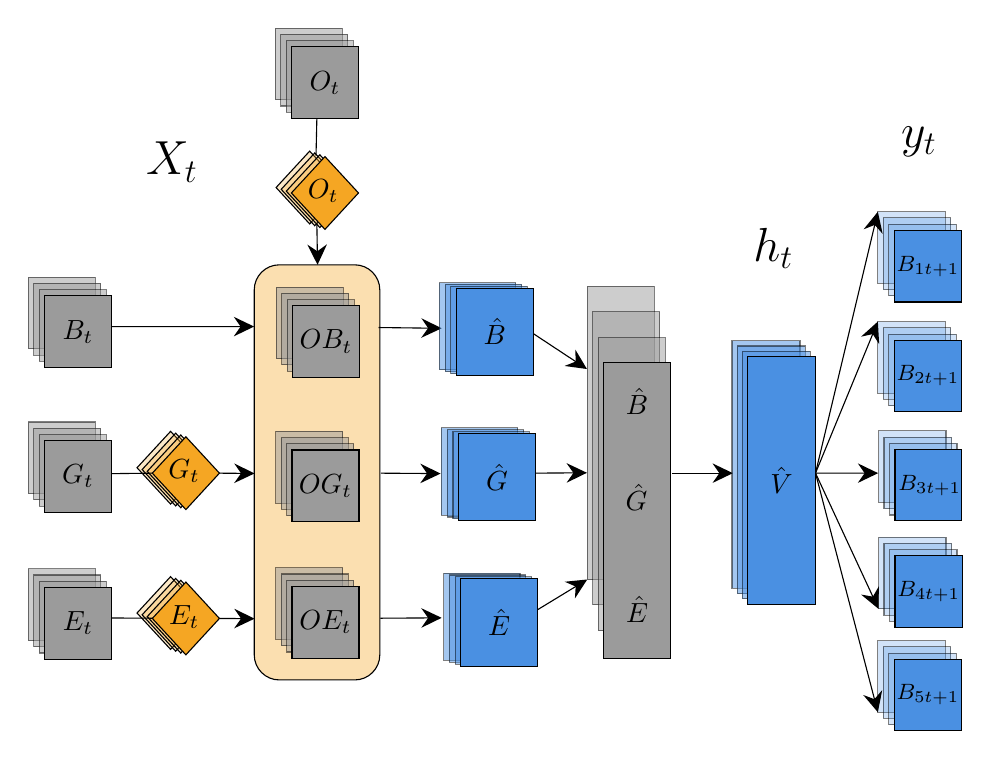
\begin{tikzpicture}[x=0.75pt,y=0.75pt,yscale=-1,xscale=1]
    %uncomment if require: \path (0,1033); %set diagram left start at 0, and has height of 1033
    
    %Rounded Rect [id:dp15650356150345013] 
    \draw  [fill={rgb, 255:red, 245; green, 166; blue, 35 }  ,fill opacity=0.36 ] (219.9,142.15) .. controls (219.9,135.47) and (225.32,130.05) .. (232,130.05) -- (268.3,130.05) .. controls (274.98,130.05) and (280.4,135.47) .. (280.4,142.15) -- (280.4,317.95) .. controls (280.4,324.63) and (274.98,330.05) .. (268.3,330.05) -- (232,330.05) .. controls (225.32,330.05) and (219.9,324.63) .. (219.9,317.95) -- cycle ;
    %Straight Lines [id:da409284418173784] 
    \draw    (250.06,109.76) -- (250.35,127.05) ;
    \draw [shift={(250.4,130.05)}, rotate = 269.03] [fill={rgb, 255:red, 0; green, 0; blue, 0 }  ][line width=0.08]  [draw opacity=0] (9.82,-4.72) -- (0,0) -- (9.82,4.72) -- (6.52,0) -- cycle    ;
    %Shape: Rectangle [id:dp7034345660290355] 
    \draw  [color={rgb, 255:red, 0; green, 0; blue, 0 }  ,draw opacity=0.5 ][fill={rgb, 255:red, 155; green, 155; blue, 155 }  ,fill opacity=0.5 ] (111.01,276.53) -- (143.26,276.53) -- (143.26,311.05) -- (111.01,311.05) -- cycle ;
    %Shape: Rectangle [id:dp22118233628007533] 
    \draw  [color={rgb, 255:red, 0; green, 0; blue, 0 }  ,draw opacity=0.5 ][fill={rgb, 255:red, 155; green, 155; blue, 155 }  ,fill opacity=0.5 ] (113.63,279.51) -- (145.88,279.51) -- (145.88,314.03) -- (113.63,314.03) -- cycle ;
    %Shape: Rectangle [id:dp24867768000931467] 
    \draw  [color={rgb, 255:red, 0; green, 0; blue, 0 }  ,draw opacity=0.5 ][fill={rgb, 255:red, 155; green, 155; blue, 155 }  ,fill opacity=0.5 ] (116.27,282.56) -- (148.53,282.56) -- (148.53,317.08) -- (116.27,317.08) -- cycle ;
    %Shape: Rectangle [id:dp124905579804508] 
    \draw  [fill={rgb, 255:red, 155; green, 155; blue, 155 }  ,fill opacity=1 ] (118.86,285.5) -- (151.11,285.5) -- (151.11,320.02) -- (118.86,320.02) -- cycle ;
    %Straight Lines [id:da8537240673366849] 
    \draw    (250.06,59.86) -- (249.67,77.43) ;
    %Shape: Rectangle [id:dp1958055080757597] 
    \draw  [color={rgb, 255:red, 0; green, 0; blue, 0 }  ,draw opacity=0.5 ][fill={rgb, 255:red, 74; green, 144; blue, 226 }  ,fill opacity=0.25 ] (520.36,157.39) -- (552.87,157.39) -- (552.87,191.9) -- (520.36,191.9) -- cycle ;
    %Shape: Rectangle [id:dp20825701586292622] 
    \draw  [color={rgb, 255:red, 0; green, 0; blue, 0 }  ,draw opacity=0.5 ][fill={rgb, 255:red, 74; green, 144; blue, 226 }  ,fill opacity=0.25 ] (523,160.37) -- (555.51,160.37) -- (555.51,194.88) -- (523,194.88) -- cycle ;
    %Shape: Rectangle [id:dp6709034910590727] 
    \draw  [color={rgb, 255:red, 0; green, 0; blue, 0 }  ,draw opacity=0.5 ][fill={rgb, 255:red, 74; green, 144; blue, 226 }  ,fill opacity=0.25 ] (525.67,163.42) -- (558.17,163.42) -- (558.17,197.93) -- (525.67,197.93) -- cycle ;
    %Shape: Rectangle [id:dp943426610209301] 
    \draw  [fill={rgb, 255:red, 74; green, 144; blue, 226 }  ,fill opacity=1 ] (528.28,166.36) -- (560.78,166.36) -- (560.78,200.87) -- (528.28,200.87) -- cycle ;
    %Shape: Rectangle [id:dp9270730461824767] 
    \draw  [color={rgb, 255:red, 0; green, 0; blue, 0 }  ,draw opacity=0.5 ][fill={rgb, 255:red, 74; green, 144; blue, 226 }  ,fill opacity=0.25 ] (520.69,210.06) -- (553.2,210.06) -- (553.2,244.56) -- (520.69,244.56) -- cycle ;
    %Shape: Rectangle [id:dp9671567967621458] 
    \draw  [color={rgb, 255:red, 0; green, 0; blue, 0 }  ,draw opacity=0.5 ][fill={rgb, 255:red, 74; green, 144; blue, 226 }  ,fill opacity=0.25 ] (523.33,213.04) -- (555.84,213.04) -- (555.84,247.54) -- (523.33,247.54) -- cycle ;
    %Shape: Rectangle [id:dp6567850092606636] 
    \draw  [color={rgb, 255:red, 0; green, 0; blue, 0 }  ,draw opacity=0.5 ][fill={rgb, 255:red, 74; green, 144; blue, 226 }  ,fill opacity=0.25 ] (526,216.09) -- (558.5,216.09) -- (558.5,250.6) -- (526,250.6) -- cycle ;
    %Shape: Rectangle [id:dp9307909660529495] 
    \draw  [fill={rgb, 255:red, 74; green, 144; blue, 226 }  ,fill opacity=1 ] (528.62,219.02) -- (560.84,219.02) -- (560.84,253.22) -- (528.62,253.22) -- cycle ;
    %Shape: Rectangle [id:dp2956426995252315] 
    \draw  [color={rgb, 255:red, 0; green, 0; blue, 0 }  ,draw opacity=0.5 ][fill={rgb, 255:red, 74; green, 144; blue, 226 }  ,fill opacity=0.25 ] (520.36,311.11) -- (552.87,311.11) -- (552.87,345.62) -- (520.36,345.62) -- cycle ;
    %Shape: Rectangle [id:dp9676718309145981] 
    \draw  [color={rgb, 255:red, 0; green, 0; blue, 0 }  ,draw opacity=0.5 ][fill={rgb, 255:red, 74; green, 144; blue, 226 }  ,fill opacity=0.25 ] (523,314.09) -- (555.51,314.09) -- (555.51,348.6) -- (523,348.6) -- cycle ;
    %Shape: Rectangle [id:dp3802447939611997] 
    \draw  [color={rgb, 255:red, 0; green, 0; blue, 0 }  ,draw opacity=0.5 ][fill={rgb, 255:red, 74; green, 144; blue, 226 }  ,fill opacity=0.25 ] (525.67,317.14) -- (558.17,317.14) -- (558.17,351.65) -- (525.67,351.65) -- cycle ;
    %Shape: Rectangle [id:dp2655409211543931] 
    \draw  [fill={rgb, 255:red, 74; green, 144; blue, 226 }  ,fill opacity=1 ] (528.28,320.08) -- (560.78,320.08) -- (560.78,354.59) -- (528.28,354.59) -- cycle ;
    %Shape: Rectangle [id:dp4040153422296009] 
    \draw  [color={rgb, 255:red, 0; green, 0; blue, 0 }  ,draw opacity=0.5 ][fill={rgb, 255:red, 74; green, 144; blue, 226 }  ,fill opacity=0.25 ] (520.69,261.32) -- (553.2,261.32) -- (553.2,295.83) -- (520.69,295.83) -- cycle ;
    %Shape: Rectangle [id:dp7066102537923638] 
    \draw  [color={rgb, 255:red, 0; green, 0; blue, 0 }  ,draw opacity=0.5 ][fill={rgb, 255:red, 74; green, 144; blue, 226 }  ,fill opacity=0.25 ] (523.33,264.3) -- (555.84,264.3) -- (555.84,298.81) -- (523.33,298.81) -- cycle ;
    %Shape: Rectangle [id:dp46050637304135866] 
    \draw  [color={rgb, 255:red, 0; green, 0; blue, 0 }  ,draw opacity=0.5 ][fill={rgb, 255:red, 74; green, 144; blue, 226 }  ,fill opacity=0.25 ] (526,267.35) -- (558.5,267.35) -- (558.5,301.86) -- (526,301.86) -- cycle ;
    %Shape: Rectangle [id:dp2033829273595421] 
    \draw  [fill={rgb, 255:red, 74; green, 144; blue, 226 }  ,fill opacity=1 ] (528.61,270.29) -- (561.11,270.29) -- (561.11,304.8) -- (528.61,304.8) -- cycle ;
    %Shape: Rectangle [id:dp19424752965877823] 
    \draw  [color={rgb, 255:red, 0; green, 0; blue, 0 }  ,draw opacity=0.5 ][fill={rgb, 255:red, 74; green, 144; blue, 226 }  ,fill opacity=0.25 ] (520.36,104.48) -- (552.87,104.48) -- (552.87,138.98) -- (520.36,138.98) -- cycle ;
    %Shape: Rectangle [id:dp6987771152166413] 
    \draw  [color={rgb, 255:red, 0; green, 0; blue, 0 }  ,draw opacity=0.5 ][fill={rgb, 255:red, 74; green, 144; blue, 226 }  ,fill opacity=0.25 ] (523,107.46) -- (555.51,107.46) -- (555.51,141.96) -- (523,141.96) -- cycle ;
    %Shape: Rectangle [id:dp12765942569283661] 
    \draw  [color={rgb, 255:red, 0; green, 0; blue, 0 }  ,draw opacity=0.5 ][fill={rgb, 255:red, 74; green, 144; blue, 226 }  ,fill opacity=0.25 ] (525.67,110.51) -- (558.17,110.51) -- (558.17,145.01) -- (525.67,145.01) -- cycle ;
    %Shape: Rectangle [id:dp16248810139444148] 
    \draw  [fill={rgb, 255:red, 74; green, 144; blue, 226 }  ,fill opacity=1 ] (528.28,113.44) -- (560.78,113.44) -- (560.78,147.95) -- (528.28,147.95) -- cycle ;
    %Shape: Rectangle [id:dp7988673729176894] 
    \draw  [color={rgb, 255:red, 0; green, 0; blue, 0 }  ,draw opacity=0.5 ][fill={rgb, 255:red, 155; green, 155; blue, 155 }  ,fill opacity=0.5 ] (111.01,205.77) -- (143.26,205.77) -- (143.26,240.29) -- (111.01,240.29) -- cycle ;
    %Shape: Rectangle [id:dp9623129937085917] 
    \draw  [color={rgb, 255:red, 0; green, 0; blue, 0 }  ,draw opacity=0.5 ][fill={rgb, 255:red, 155; green, 155; blue, 155 }  ,fill opacity=0.5 ] (113.63,208.75) -- (145.88,208.75) -- (145.88,243.27) -- (113.63,243.27) -- cycle ;
    %Shape: Rectangle [id:dp429379441325212] 
    \draw  [color={rgb, 255:red, 0; green, 0; blue, 0 }  ,draw opacity=0.5 ][fill={rgb, 255:red, 155; green, 155; blue, 155 }  ,fill opacity=0.5 ] (116.27,211.8) -- (148.53,211.8) -- (148.53,246.32) -- (116.27,246.32) -- cycle ;
    %Shape: Rectangle [id:dp9493890675957639] 
    \draw  [fill={rgb, 255:red, 155; green, 155; blue, 155 }  ,fill opacity=1 ] (118.86,214.74) -- (151.11,214.74) -- (151.11,249.26) -- (118.86,249.26) -- cycle ;
    %Straight Lines [id:da0399560958706785] 
    \draw [fill={rgb, 255:red, 155; green, 155; blue, 155 }  ,fill opacity=1 ]   (150.09,159.83) -- (216.85,159.8) ;
    \draw [shift={(219.85,159.8)}, rotate = 179.98] [fill={rgb, 255:red, 0; green, 0; blue, 0 }  ][line width=0.08]  [draw opacity=0] (9.82,-4.72) -- (0,0) -- (9.82,4.72) -- (6.52,0) -- cycle    ;
    %Shape: Rectangle [id:dp3393145890474042] 
    \draw  [color={rgb, 255:red, 0; green, 0; blue, 0 }  ,draw opacity=0.5 ][fill={rgb, 255:red, 155; green, 155; blue, 155 }  ,fill opacity=0.5 ] (111.01,136.06) -- (143.26,136.06) -- (143.26,170.57) -- (111.01,170.57) -- cycle ;
    %Shape: Rectangle [id:dp27631704382885136] 
    \draw  [color={rgb, 255:red, 0; green, 0; blue, 0 }  ,draw opacity=0.5 ][fill={rgb, 255:red, 155; green, 155; blue, 155 }  ,fill opacity=0.5 ] (113.63,139.04) -- (145.88,139.04) -- (145.88,173.55) -- (113.63,173.55) -- cycle ;
    %Shape: Rectangle [id:dp8553441662393909] 
    \draw  [color={rgb, 255:red, 0; green, 0; blue, 0 }  ,draw opacity=0.5 ][fill={rgb, 255:red, 155; green, 155; blue, 155 }  ,fill opacity=0.5 ] (116.27,142.09) -- (148.53,142.09) -- (148.53,176.61) -- (116.27,176.61) -- cycle ;
    %Shape: Rectangle [id:dp4571491350911555] 
    \draw  [fill={rgb, 255:red, 155; green, 155; blue, 155 }  ,fill opacity=1 ] (118.86,145.03) -- (151.11,145.03) -- (151.11,179.54) -- (118.86,179.54) -- cycle ;
    %Shape: Diamond [id:dp42134346339770745] 
    \draw  [fill={rgb, 255:red, 245; green, 166; blue, 35 }  ,fill opacity=0.25 ] (179.6,210.28) -- (195.77,227.81) -- (179.6,245.33) -- (163.43,227.81) -- cycle ;
    %Shape: Diamond [id:dp8160874162123375] 
    \draw  [fill={rgb, 255:red, 245; green, 166; blue, 35 }  ,fill opacity=0.25 ] (182.05,211.16) -- (198.22,228.68) -- (182.05,246.2) -- (165.89,228.68) -- cycle ;
    %Shape: Diamond [id:dp05986250472128074] 
    \draw  [fill={rgb, 255:red, 245; green, 166; blue, 35 }  ,fill opacity=0.25 ] (184.51,212.04) -- (200.68,229.56) -- (184.51,247.08) -- (168.34,229.56) -- cycle ;
    %Shape: Diamond [id:dp6831575900746938] 
    \draw  [fill={rgb, 255:red, 245; green, 166; blue, 35 }  ,fill opacity=1 ] (186.97,212.91) -- (203.13,230.43) -- (186.97,247.96) -- (170.8,230.43) -- cycle ;
    %Straight Lines [id:da3169233008507637] 
    \draw    (151.46,230.66) -- (170.8,230.43) ;
    %Shape: Diamond [id:dp08100159339963764] 
    \draw  [fill={rgb, 255:red, 245; green, 166; blue, 35 }  ,fill opacity=0.25 ] (179.6,280.28) -- (195.77,297.81) -- (179.6,315.33) -- (163.43,297.81) -- cycle ;
    %Shape: Diamond [id:dp6545409040088919] 
    \draw  [fill={rgb, 255:red, 245; green, 166; blue, 35 }  ,fill opacity=0.25 ] (182.05,281.16) -- (198.22,298.68) -- (182.05,316.2) -- (165.89,298.68) -- cycle ;
    %Shape: Diamond [id:dp22008618792927115] 
    \draw  [fill={rgb, 255:red, 245; green, 166; blue, 35 }  ,fill opacity=0.25 ] (184.51,282.04) -- (200.68,299.56) -- (184.51,317.08) -- (168.34,299.56) -- cycle ;
    %Shape: Diamond [id:dp6216162169932065] 
    \draw  [fill={rgb, 255:red, 245; green, 166; blue, 35 }  ,fill opacity=1 ] (186.97,282.91) -- (203.13,300.43) -- (186.97,317.96) -- (170.8,300.43) -- cycle ;
    %Straight Lines [id:da6348314705630924] 
    \draw    (203.13,300.43) -- (217.07,300.51) ;
    \draw [shift={(220.07,300.53)}, rotate = 180.32] [fill={rgb, 255:red, 0; green, 0; blue, 0 }  ][line width=0.08]  [draw opacity=0] (9.82,-4.72) -- (0,0) -- (9.82,4.72) -- (6.52,0) -- cycle    ;
    %Straight Lines [id:da29443986089740126] 
    \draw    (150.89,300.2) -- (170.89,300.31) ;
    %Straight Lines [id:da7037674707293678] 
    \draw [fill={rgb, 255:red, 155; green, 155; blue, 155 }  ,fill opacity=1 ]   (279.77,160.26) -- (307.2,160.6) ;
    \draw [shift={(310.2,160.63)}, rotate = 180.71] [fill={rgb, 255:red, 0; green, 0; blue, 0 }  ][line width=0.08]  [draw opacity=0] (9.82,-4.72) -- (0,0) -- (9.82,4.72) -- (6.52,0) -- cycle    ;
    %Straight Lines [id:da04725287763752273] 
    \draw [fill={rgb, 255:red, 155; green, 155; blue, 155 }  ,fill opacity=1 ]   (350.2,160.45) -- (377.7,178.6) ;
    \draw [shift={(380.2,180.25)}, rotate = 213.42] [fill={rgb, 255:red, 0; green, 0; blue, 0 }  ][line width=0.08]  [draw opacity=0] (9.82,-4.72) -- (0,0) -- (9.82,4.72) -- (6.52,0) -- cycle    ;
    %Straight Lines [id:da6945773359077246] 
    \draw    (203.13,230.43) -- (217.07,230.54) ;
    \draw [shift={(220.07,230.56)}, rotate = 180.44] [fill={rgb, 255:red, 0; green, 0; blue, 0 }  ][line width=0.08]  [draw opacity=0] (9.82,-4.72) -- (0,0) -- (9.82,4.72) -- (6.52,0) -- cycle    ;
    %Straight Lines [id:da6273046628189572] 
    \draw [fill={rgb, 255:red, 155; green, 155; blue, 155 }  ,fill opacity=1 ]   (280.91,230.43) -- (306.7,230.61) ;
    \draw [shift={(309.7,230.63)}, rotate = 180.41] [fill={rgb, 255:red, 0; green, 0; blue, 0 }  ][line width=0.08]  [draw opacity=0] (9.82,-4.72) -- (0,0) -- (9.82,4.72) -- (6.52,0) -- cycle    ;
    %Straight Lines [id:da5724582303552335] 
    \draw [fill={rgb, 255:red, 155; green, 155; blue, 155 }  ,fill opacity=1 ]   (280.63,300.31) -- (307.2,300.15) ;
    \draw [shift={(310.2,300.13)}, rotate = 179.65] [fill={rgb, 255:red, 0; green, 0; blue, 0 }  ][line width=0.08]  [draw opacity=0] (9.82,-4.72) -- (0,0) -- (9.82,4.72) -- (6.52,0) -- cycle    ;
    %Shape: Rectangle [id:dp53907172122875] 
    \draw  [color={rgb, 255:red, 0; green, 0; blue, 0 }  ,draw opacity=0.5 ][fill={rgb, 255:red, 155; green, 155; blue, 155 }  ,fill opacity=0.5 ] (230.01,16.06) -- (262.26,16.06) -- (262.26,50.57) -- (230.01,50.57) -- cycle ;
    %Shape: Rectangle [id:dp009192212091793661] 
    \draw  [color={rgb, 255:red, 0; green, 0; blue, 0 }  ,draw opacity=0.5 ][fill={rgb, 255:red, 155; green, 155; blue, 155 }  ,fill opacity=0.5 ] (232.63,19.04) -- (264.88,19.04) -- (264.88,53.55) -- (232.63,53.55) -- cycle ;
    %Shape: Rectangle [id:dp10982806096562447] 
    \draw  [color={rgb, 255:red, 0; green, 0; blue, 0 }  ,draw opacity=0.5 ][fill={rgb, 255:red, 155; green, 155; blue, 155 }  ,fill opacity=0.5 ] (235.27,22.09) -- (267.53,22.09) -- (267.53,56.61) -- (235.27,56.61) -- cycle ;
    %Shape: Rectangle [id:dp024787601372134982] 
    \draw  [fill={rgb, 255:red, 155; green, 155; blue, 155 }  ,fill opacity=1 ] (237.86,25.03) -- (270.11,25.03) -- (270.11,59.54) -- (237.86,59.54) -- cycle ;
    %Shape: Rectangle [id:dp9022114030928725] 
    \draw  [color={rgb, 255:red, 0; green, 0; blue, 0 }  ,draw opacity=0.5 ][fill={rgb, 255:red, 155; green, 155; blue, 155 }  ,fill opacity=0.5 ] (380.34,140.45) -- (412.6,140.45) -- (412.6,281.66) -- (380.34,281.66) -- cycle ;
    %Shape: Rectangle [id:dp9877830883323443] 
    \draw  [color={rgb, 255:red, 0; green, 0; blue, 0 }  ,draw opacity=0.5 ][fill={rgb, 255:red, 155; green, 155; blue, 155 }  ,fill opacity=0.5 ] (382.96,152.64) -- (415.22,152.64) -- (415.22,293.84) -- (382.96,293.84) -- cycle ;
    %Shape: Rectangle [id:dp8814167498359042] 
    \draw  [color={rgb, 255:red, 0; green, 0; blue, 0 }  ,draw opacity=0.5 ][fill={rgb, 255:red, 155; green, 155; blue, 155 }  ,fill opacity=0.5 ] (385.61,165.13) -- (417.86,165.13) -- (417.86,306.34) -- (385.61,306.34) -- cycle ;
    %Shape: Rectangle [id:dp5289911737134959] 
    \draw  [fill={rgb, 255:red, 155; green, 155; blue, 155 }  ,fill opacity=1 ] (388.19,177.14) -- (420.45,177.14) -- (420.45,319.53) -- (388.19,319.53) -- cycle ;
    %Shape: Rectangle [id:dp8149328215662492] 
    \draw  [color={rgb, 255:red, 0; green, 0; blue, 0 }  ,draw opacity=0.5 ][fill={rgb, 255:red, 155; green, 155; blue, 155 }  ,fill opacity=0.5 ] (230.51,140.77) -- (262.76,140.77) -- (262.76,175.29) -- (230.51,175.29) -- cycle ;
    %Shape: Rectangle [id:dp45921305478843055] 
    \draw  [color={rgb, 255:red, 0; green, 0; blue, 0 }  ,draw opacity=0.5 ][fill={rgb, 255:red, 155; green, 155; blue, 155 }  ,fill opacity=0.5 ] (233.13,143.75) -- (265.38,143.75) -- (265.38,178.27) -- (233.13,178.27) -- cycle ;
    %Shape: Rectangle [id:dp6228279530655318] 
    \draw  [color={rgb, 255:red, 0; green, 0; blue, 0 }  ,draw opacity=0.5 ][fill={rgb, 255:red, 155; green, 155; blue, 155 }  ,fill opacity=0.5 ] (235.77,146.8) -- (268.03,146.8) -- (268.03,181.32) -- (235.77,181.32) -- cycle ;
    %Shape: Rectangle [id:dp3598797805540589] 
    \draw  [fill={rgb, 255:red, 155; green, 155; blue, 155 }  ,fill opacity=1 ] (238.36,149.74) -- (270.61,149.74) -- (270.61,184.26) -- (238.36,184.26) -- cycle ;
    %Shape: Rectangle [id:dp9661891091990619] 
    \draw  [color={rgb, 255:red, 0; green, 0; blue, 0 }  ,draw opacity=0.5 ][fill={rgb, 255:red, 155; green, 155; blue, 155 }  ,fill opacity=0.5 ] (230.26,210.32) -- (262.51,210.32) -- (262.51,244.84) -- (230.26,244.84) -- cycle ;
    %Shape: Rectangle [id:dp690231151268716] 
    \draw  [color={rgb, 255:red, 0; green, 0; blue, 0 }  ,draw opacity=0.5 ][fill={rgb, 255:red, 155; green, 155; blue, 155 }  ,fill opacity=0.5 ] (232.88,213.3) -- (265.13,213.3) -- (265.13,247.82) -- (232.88,247.82) -- cycle ;
    %Shape: Rectangle [id:dp48804619093484347] 
    \draw  [color={rgb, 255:red, 0; green, 0; blue, 0 }  ,draw opacity=0.5 ][fill={rgb, 255:red, 155; green, 155; blue, 155 }  ,fill opacity=0.5 ] (235.52,216.35) -- (267.78,216.35) -- (267.78,250.87) -- (235.52,250.87) -- cycle ;
    %Shape: Rectangle [id:dp22992925838286216] 
    \draw  [fill={rgb, 255:red, 155; green, 155; blue, 155 }  ,fill opacity=1 ] (238.11,219.29) -- (270.36,219.29) -- (270.36,253.81) -- (238.11,253.81) -- cycle ;
    %Shape: Rectangle [id:dp29039742489844134] 
    \draw  [color={rgb, 255:red, 0; green, 0; blue, 0 }  ,draw opacity=0.5 ][fill={rgb, 255:red, 155; green, 155; blue, 155 }  ,fill opacity=0.5 ] (230.26,276.02) -- (262.51,276.02) -- (262.51,310.54) -- (230.26,310.54) -- cycle ;
    %Shape: Rectangle [id:dp42091335353816794] 
    \draw  [color={rgb, 255:red, 0; green, 0; blue, 0 }  ,draw opacity=0.5 ][fill={rgb, 255:red, 155; green, 155; blue, 155 }  ,fill opacity=0.5 ] (232.88,279) -- (265.13,279) -- (265.13,313.52) -- (232.88,313.52) -- cycle ;
    %Shape: Rectangle [id:dp9855473947081604] 
    \draw  [color={rgb, 255:red, 0; green, 0; blue, 0 }  ,draw opacity=0.5 ][fill={rgb, 255:red, 155; green, 155; blue, 155 }  ,fill opacity=0.5 ] (235.52,282.05) -- (267.78,282.05) -- (267.78,316.57) -- (235.52,316.57) -- cycle ;
    %Shape: Rectangle [id:dp434232717458334] 
    \draw  [fill={rgb, 255:red, 155; green, 155; blue, 155 }  ,fill opacity=1 ] (238.11,284.99) -- (270.36,284.99) -- (270.36,319.51) -- (238.11,319.51) -- cycle ;
    %Shape: Diamond [id:dp30872576312410427] 
    \draw  [fill={rgb, 255:red, 245; green, 166; blue, 35 }  ,fill opacity=0.25 ] (246.6,75.28) -- (262.77,92.81) -- (246.6,110.33) -- (230.43,92.81) -- cycle ;
    %Shape: Diamond [id:dp6849972388912634] 
    \draw  [fill={rgb, 255:red, 245; green, 166; blue, 35 }  ,fill opacity=0.25 ] (249.05,76.16) -- (265.22,93.68) -- (249.05,111.2) -- (232.89,93.68) -- cycle ;
    %Shape: Diamond [id:dp857485897511279] 
    \draw  [fill={rgb, 255:red, 245; green, 166; blue, 35 }  ,fill opacity=0.25 ] (251.51,77.04) -- (267.68,94.56) -- (251.51,112.08) -- (235.34,94.56) -- cycle ;
    %Shape: Diamond [id:dp49326046176048577] 
    \draw  [fill={rgb, 255:red, 245; green, 166; blue, 35 }  ,fill opacity=1 ] (253.97,77.91) -- (270.13,95.43) -- (253.97,112.96) -- (237.8,95.43) -- cycle ;
    %Straight Lines [id:da9533396825264671] 
    \draw [fill={rgb, 255:red, 155; green, 155; blue, 155 }  ,fill opacity=1 ]   (349.2,230.45) -- (377.2,230.27) ;
    \draw [shift={(380.2,230.25)}, rotate = 179.63] [fill={rgb, 255:red, 0; green, 0; blue, 0 }  ][line width=0.08]  [draw opacity=0] (9.82,-4.72) -- (0,0) -- (9.82,4.72) -- (6.52,0) -- cycle    ;
    %Straight Lines [id:da46693829157920863] 
    \draw [fill={rgb, 255:red, 155; green, 155; blue, 155 }  ,fill opacity=1 ]   (350.4,299.88) -- (377.78,283.22) ;
    \draw [shift={(380.34,281.66)}, rotate = 148.68] [fill={rgb, 255:red, 0; green, 0; blue, 0 }  ][line width=0.08]  [draw opacity=0] (9.82,-4.72) -- (0,0) -- (9.82,4.72) -- (6.52,0) -- cycle    ;
    %Straight Lines [id:da9477168442608538] 
    \draw [fill={rgb, 255:red, 155; green, 155; blue, 155 }  ,fill opacity=1 ]   (421.09,230.43) -- (447.51,230.43) ;
    \draw [shift={(450.51,230.43)}, rotate = 180] [fill={rgb, 255:red, 0; green, 0; blue, 0 }  ][line width=0.08]  [draw opacity=0] (9.82,-4.72) -- (0,0) -- (9.82,4.72) -- (6.52,0) -- cycle    ;
    %Straight Lines [id:da17588566125157779] 
    \draw [fill={rgb, 255:red, 155; green, 155; blue, 155 }  ,fill opacity=1 ]   (490.32,230.39) -- (517.51,230.42) ;
    \draw [shift={(520.51,230.43)}, rotate = 180.08] [fill={rgb, 255:red, 0; green, 0; blue, 0 }  ][line width=0.08]  [draw opacity=0] (9.82,-4.72) -- (0,0) -- (9.82,4.72) -- (6.52,0) -- cycle    ;
    %Straight Lines [id:da990575471229112] 
    \draw [fill={rgb, 255:red, 155; green, 155; blue, 155 }  ,fill opacity=1 ]   (490.32,230.39) -- (519.43,293.11) ;
    \draw [shift={(520.69,295.83)}, rotate = 245.1] [fill={rgb, 255:red, 0; green, 0; blue, 0 }  ][line width=0.08]  [draw opacity=0] (9.82,-4.72) -- (0,0) -- (9.82,4.72) -- (6.52,0) -- cycle    ;
    %Straight Lines [id:da11726542356327818] 
    \draw [fill={rgb, 255:red, 155; green, 155; blue, 155 }  ,fill opacity=1 ]   (490.32,230.39) -- (519.61,342.72) ;
    \draw [shift={(520.36,345.62)}, rotate = 255.39] [fill={rgb, 255:red, 0; green, 0; blue, 0 }  ][line width=0.08]  [draw opacity=0] (9.82,-4.72) -- (0,0) -- (9.82,4.72) -- (6.52,0) -- cycle    ;
    %Straight Lines [id:da6006783627611112] 
    \draw [fill={rgb, 255:red, 155; green, 155; blue, 155 }  ,fill opacity=1 ]   (490.32,230.39) -- (519.22,160.17) ;
    \draw [shift={(520.36,157.39)}, rotate = 112.37] [fill={rgb, 255:red, 0; green, 0; blue, 0 }  ][line width=0.08]  [draw opacity=0] (9.82,-4.72) -- (0,0) -- (9.82,4.72) -- (6.52,0) -- cycle    ;
    %Straight Lines [id:da16067428057688105] 
    \draw [fill={rgb, 255:red, 155; green, 155; blue, 155 }  ,fill opacity=1 ]   (490.32,230.39) -- (519.67,107.4) ;
    \draw [shift={(520.36,104.48)}, rotate = 103.42] [fill={rgb, 255:red, 0; green, 0; blue, 0 }  ][line width=0.08]  [draw opacity=0] (9.82,-4.72) -- (0,0) -- (9.82,4.72) -- (6.52,0) -- cycle    ;
    %Shape: Rectangle [id:dp04777231109494484] 
    \draw  [color={rgb, 255:red, 0; green, 0; blue, 0 }  ,draw opacity=0.5 ][fill={rgb, 255:red, 74; green, 144; blue, 226 }  ,fill opacity=0.5 ] (309.1,138.6) -- (345.95,138.6) -- (345.95,180.65) -- (309.1,180.65) -- cycle ;
    %Shape: Rectangle [id:dp7558311796324689] 
    \draw  [color={rgb, 255:red, 0; green, 0; blue, 0 }  ,draw opacity=0.5 ][fill={rgb, 255:red, 74; green, 144; blue, 226 }  ,fill opacity=0.5 ] (311.88,139.51) -- (348.73,139.51) -- (348.73,181.56) -- (311.88,181.56) -- cycle ;
    %Shape: Rectangle [id:dp02297715036875614] 
    \draw  [color={rgb, 255:red, 0; green, 0; blue, 0 }  ,draw opacity=0.5 ][fill={rgb, 255:red, 74; green, 144; blue, 226 }  ,fill opacity=0.5 ] (314.67,140.42) -- (351.51,140.42) -- (351.51,182.46) -- (314.67,182.46) -- cycle ;
    %Shape: Rectangle [id:dp7483619990673073] 
    \draw  [fill={rgb, 255:red, 74; green, 144; blue, 226 }  ,fill opacity=1 ] (317.45,141.33) -- (354.29,141.33) -- (354.29,183.37) -- (317.45,183.37) -- cycle ;
    %Shape: Rectangle [id:dp8163589302848298] 
    \draw  [color={rgb, 255:red, 0; green, 0; blue, 0 }  ,draw opacity=0.5 ][fill={rgb, 255:red, 74; green, 144; blue, 226 }  ,fill opacity=0.5 ] (450.1,166.6) -- (482.87,166.6) -- (482.87,285.87) -- (450.1,285.87) -- cycle ;
    %Shape: Rectangle [id:dp13561622734198409] 
    \draw  [color={rgb, 255:red, 0; green, 0; blue, 0 }  ,draw opacity=0.5 ][fill={rgb, 255:red, 74; green, 144; blue, 226 }  ,fill opacity=0.5 ] (452.57,169.18) -- (485.34,169.18) -- (485.34,288.44) -- (452.57,288.44) -- cycle ;
    %Shape: Rectangle [id:dp028266783786446537] 
    \draw  [color={rgb, 255:red, 0; green, 0; blue, 0 }  ,draw opacity=0.5 ][fill={rgb, 255:red, 74; green, 144; blue, 226 }  ,fill opacity=0.5 ] (455.05,171.76) -- (487.82,171.76) -- (487.82,291.02) -- (455.05,291.02) -- cycle ;
    %Shape: Rectangle [id:dp501556684499422] 
    \draw  [fill={rgb, 255:red, 74; green, 144; blue, 226 }  ,fill opacity=1 ] (457.52,174.33) -- (490.29,174.33) -- (490.29,293.6) -- (457.52,293.6) -- cycle ;
    
    %Shape: Rectangle [id:dp3431119253458095] 
    \draw  [color={rgb, 255:red, 0; green, 0; blue, 0 }  ,draw opacity=0.5 ][fill={rgb, 255:red, 74; green, 144; blue, 226 }  ,fill opacity=0.5 ] (310.1,208.6) -- (346.95,208.6) -- (346.95,250.65) -- (310.1,250.65) -- cycle ;
    %Shape: Rectangle [id:dp8294825257941912] 
    \draw  [color={rgb, 255:red, 0; green, 0; blue, 0 }  ,draw opacity=0.5 ][fill={rgb, 255:red, 74; green, 144; blue, 226 }  ,fill opacity=0.5 ] (312.88,209.51) -- (349.73,209.51) -- (349.73,251.56) -- (312.88,251.56) -- cycle ;
    %Shape: Rectangle [id:dp049289680132614255] 
    \draw  [color={rgb, 255:red, 0; green, 0; blue, 0 }  ,draw opacity=0.5 ][fill={rgb, 255:red, 74; green, 144; blue, 226 }  ,fill opacity=0.5 ] (315.67,210.42) -- (352.51,210.42) -- (352.51,252.46) -- (315.67,252.46) -- cycle ;
    %Shape: Rectangle [id:dp4657902939703581] 
    \draw  [fill={rgb, 255:red, 74; green, 144; blue, 226 }  ,fill opacity=1 ] (318.45,211.33) -- (355.29,211.33) -- (355.29,253.37) -- (318.45,253.37) -- cycle ;
    %Shape: Rectangle [id:dp8549615376830864] 
    \draw  [color={rgb, 255:red, 0; green, 0; blue, 0 }  ,draw opacity=0.5 ][fill={rgb, 255:red, 74; green, 144; blue, 226 }  ,fill opacity=0.5 ] (311.1,278.6) -- (347.95,278.6) -- (347.95,320.65) -- (311.1,320.65) -- cycle ;
    %Shape: Rectangle [id:dp07757251126817089] 
    \draw  [color={rgb, 255:red, 0; green, 0; blue, 0 }  ,draw opacity=0.5 ][fill={rgb, 255:red, 74; green, 144; blue, 226 }  ,fill opacity=0.5 ] (313.88,279.51) -- (350.73,279.51) -- (350.73,321.56) -- (313.88,321.56) -- cycle ;
    %Shape: Rectangle [id:dp9077595517238054] 
    \draw  [color={rgb, 255:red, 0; green, 0; blue, 0 }  ,draw opacity=0.5 ][fill={rgb, 255:red, 74; green, 144; blue, 226 }  ,fill opacity=0.5 ] (316.67,280.42) -- (353.51,280.42) -- (353.51,322.46) -- (316.67,322.46) -- cycle ;
    %Shape: Rectangle [id:dp2039123260975314] 
    \draw  [fill={rgb, 255:red, 74; green, 144; blue, 226 }  ,fill opacity=1 ] (319.45,281.33) -- (356.29,281.33) -- (356.29,323.37) -- (319.45,323.37) -- cycle ;
    
    % Text Node
    \draw (134.99,302.76) node  [font=\normalsize]  {$E_{t}$};
    % Text Node
    \draw (180.34,80.58) node  [font=\LARGE]  {$X_{t}$};
    % Text Node
    \draw (470.01,121.94) node  [font=\LARGE]  {$h_{t}$};
    % Text Node
    \draw (544.53,183.61) node  [font=\footnotesize]  {$B_{2t+1}$};
    % Text Node
    \draw (545.41,236.28) node  [font=\footnotesize]  {$B_{3t+1}$};
    % Text Node
    \draw (544.86,287.54) node  [font=\footnotesize]  {$B_{4t+1}$};
    % Text Node
    \draw (544.53,337.33) node  [font=\footnotesize]  {$B_{5t+1}$};
    % Text Node
    \draw (540.21,70.84) node  [font=\LARGE]  {$y_{t}$};
    % Text Node
    \draw (544.53,130.7) node  [font=\footnotesize]  {$B_{1t+1}$};
    % Text Node
    \draw (134.99,232) node  [font=\normalsize]  {$G_{t}$};
    % Text Node
    \draw (134.99,162.29) node  [font=\normalsize]  {$B_{t}$};
    % Text Node
    \draw (186.15,229.56) node  [font=\normalsize]  {$G_{t}$};
    % Text Node
    \draw (186.15,299.56) node  [font=\normalsize]  {$E_{t}$};
    % Text Node
    \draw (253.99,42.29) node  [font=\normalsize]  {$O_{t}$};
    % Text Node
    \draw (254.49,167) node  [font=\normalsize]  {$OB_{t}$};
    % Text Node
    \draw (254.24,236.55) node  [font=\normalsize]  {$OG_{t}$};
    % Text Node
    \draw (254.24,302.25) node  [font=\normalsize]  {$OE_{t}$};
    % Text Node
    \draw (253.15,94.56) node  [font=\normalsize]  {$O_{t}$};
    % Text Node
    \draw (404.35,195.78) node  [font=\normalsize]  {$\hat{B}$};
    % Text Node
    \draw (404.07,242.06) node  [font=\normalsize]  {$\hat{G}$};
    % Text Node
    \draw (404.35,296.11) node  [font=\normalsize]  {$\hat{E}$};
    % Text Node
    \draw (473.91,233.97) node  [font=\normalsize]  {$\hat{V}$};
    % Text Node
    \draw (335.87,162.35) node  [font=\normalsize]  {$\hat{B}$};
    % Text Node
    \draw (336.87,232.35) node  [font=\normalsize]  {$\hat{G}$};
    % Text Node
    \draw (337.87,302.35) node  [font=\normalsize]  {$\hat{E}$};
    
    
    \end{tikzpicture}



\end{adjustbox}
\end{center}
\caption[\textbf{The environment-event time distributed multi layer perceptron architecture}]{Blue and orange shapes represent respectively feedforward and embedding operations. Gray shapes indicate operations with no learnable parameters, such as tensor instantiation and concatenation. Stacked, transparent colouring indicates tensors with a sequential structure. Straight arrows refer to the presence of feed-forward information flow. All the feedforward operations are time distributed.}
\label{fig: mlp_3}
\end{figure}

\subsection{Data}
\label{data_3}
\begin{table*}[h]
\centering
\caption{Descriptive Statistics of Considered Metrics and Games}
\label{game_description_33}
  \begin{tabularx}{\textwidth}{cccccccX}
  \toprule
  \multirow{2}{*}{\textbf{Game}} &
   \multirow{2}{*}{\textbf{\begin{tabular}[c]{@{}c@{}}Sample \\ Size\end{tabular}}} &
   \textbf{\begin{tabular}[c]{@{}c@{}}Number \\ of \\ Sessions\end{tabular}} &
   \textbf{\begin{tabular}[c]{@{}c@{}}Absence \\ (minutes)\end{tabular}} &
   \textbf{\begin{tabular}[c]{@{}c@{}}Session \\ Time\\ (minutes)\end{tabular}} &
   \textbf{\begin{tabular}[c]{@{}c@{}}Active \\ Time\\ (\% Session Time)\end{tabular}} &
   \textbf{\begin{tabular}[c]{@{}c@{}}Session \\ Activity\end{tabular}} &
   \multirow{2}{*}{\textbf{\begin{tabularx}{\textwidth}[X]{@{}c@{}} Type \end{tabularx}}} \\ \midrule
   &
    &
   \multicolumn{5}{c}{\textbf{\begin{tabular}[c]{@{}c@{}}(Median $\pm$ IQR)\end{tabular}}} &
    \\ \midrule
  \textbf{hmg} &
   452,386 &
   \begin{tabular}[c]{@{}c@{}}5 $\pm$ 6\end{tabular} &
   \begin{tabular}[c]{@{}c@{}}141$\pm$ 219\end{tabular} &
   \begin{tabular}[c]{@{}c@{}}12 $\pm$ 15 \end{tabular} &
   \begin{tabular}[c]{@{}c@{}}87 $\pm$  24 \end{tabular} &
   \begin{tabular}[c]{@{}c@{}}1.3 $\pm$  0.9\end{tabular} &
   \begin{tabular}[c]{@{}c@{}}Mobile\\ Strategy\end{tabular} \\
  \textbf{jc3} &
   491,329 &
   \begin{tabular}[c]{@{}c@{}}7 $\pm$ 7\end{tabular} &
   \begin{tabular}[c]{@{}c@{}}27 $\pm$ 365\end{tabular} &
   \begin{tabular}[c]{@{}c@{}}64 $\pm$ 143\end{tabular} &
   \begin{tabular}[c]{@{}c@{}}99 $\pm$ 1\end{tabular} &
   \begin{tabular}[c]{@{}c@{}}0.18 $\pm$ 0.22 \end{tabular} &
   \begin{tabular}[c]{@{}c@{}}Console\\ Action\\Open\\World\end{tabular} \\
  \textbf{jc4} &
   485,276 &
   \begin{tabular}[c]{@{}c@{}}6 $\pm$ 7\end{tabular} &
   \begin{tabular}[c]{@{}c@{}}31 $\pm$ 356\end{tabular} &
   \begin{tabular}[c]{@{}c@{}}59 $\pm$ 87\end{tabular} &
   \begin{tabular}[c]{@{}c@{}}82 $\pm$ 25\end{tabular} &
   \begin{tabular}[c]{@{}c@{}}0.28 $\pm$ 0.45\end{tabular} &
   \begin{tabular}[c]{@{}c@{}}Console\\ Action\\Open\\World\end{tabular} \\
  \textbf{lis} &
   483,783 &
   \begin{tabular}[c]{@{}c@{}}5 $\pm$ 6 \end{tabular} &
   \begin{tabular}[c]{@{}c@{}}70 $\pm$ 844\end{tabular} &
   \begin{tabular}[c]{@{}c@{}}64 $\pm$ 104\end{tabular} &
   \begin{tabular}[c]{@{}c@{}}78 $\pm$ 25\end{tabular} &
   \begin{tabular}[c]{@{}c@{}}0.5 $\pm$ 0.4\end{tabular} &
   \begin{tabular}[c]{@{}c@{}}Console\\ Graphic\\ Adventure\end{tabular} \\
  \textbf{lisbf} &
   431,355 &
   \begin{tabular}[c]{@{}c@{}}6 $\pm$ 6\end{tabular} &
   \begin{tabular}[c]{@{}c@{}}173  $\pm$ 574\end{tabular} &
   \begin{tabular}[c]{@{}c@{}}67 $\pm$ 87\end{tabular} &
   \begin{tabular}[c]{@{}c@{}}81 $\pm$ 26\end{tabular} &
   \begin{tabular}[c]{@{}c@{}}0.08 $\pm$ 0.15\end{tabular} &
   \begin{tabular}[c]{@{}c@{}}Console\\ Graphic\\ Adventure\end{tabular} \\
  \textbf{outr} &
   461,823 &
   \begin{tabular}[c]{@{}c@{}}7 $\pm$ 7\end{tabular} &
   \begin{tabular}[c]{@{}c@{}}47 $\pm$ 33\end{tabular} &
   \begin{tabular}[c]{@{}c@{}}64 $\pm$ 121\end{tabular} &
   \begin{tabular}[c]{@{}c@{}}88 $\pm$ 65\end{tabular} &
   \begin{tabular}[c]{@{}c@{}}0.02 $\pm$ 0.04\end{tabular} &
   \begin{tabular}[c]{@{}c@{}}Console\\ Action\\Open\\World\\Co-op\end{tabular} \\ \bottomrule
  \end{tabularx}
\end{table*}
\begin{table}[H] \centering
\caption{Description of Selected Telemetries}
\label{metricsdescription_3}
  \begin{tabularx}{\textwidth}{@{}lX@{}}
    \toprule
    \textbf{Metric}      & \textbf{Description}          \\ \midrule
    {Absence}    & Temporal distance between sessions (hours)  \\
    {Session Time}     & Overall session duration (minutes)       \\ 
    {Active Time}      & Percentage of Session Time actively playing  \\ 
    {Session Activity}    & Ratio of user initiated gameplay-related actions per minute in Session Time. E.g.\\ 
                & "Attack an enemy" is considered a valid\\ 
                & action while "Being attacked by an enemy" is not.\\
    {N°Sessions}    & Number of played sessions.\\ 
    {Object}    &  Game object identifier.  \\
    \bottomrule
  \end{tabularx}
\end{table}
\lorem

\subsection{Model Tuning and Comparison}
\label{tuning_comparison_3}
\lorem

\subsection{Results}
\label{results_3}
\lorem
\begin{figure}[h]
\centering
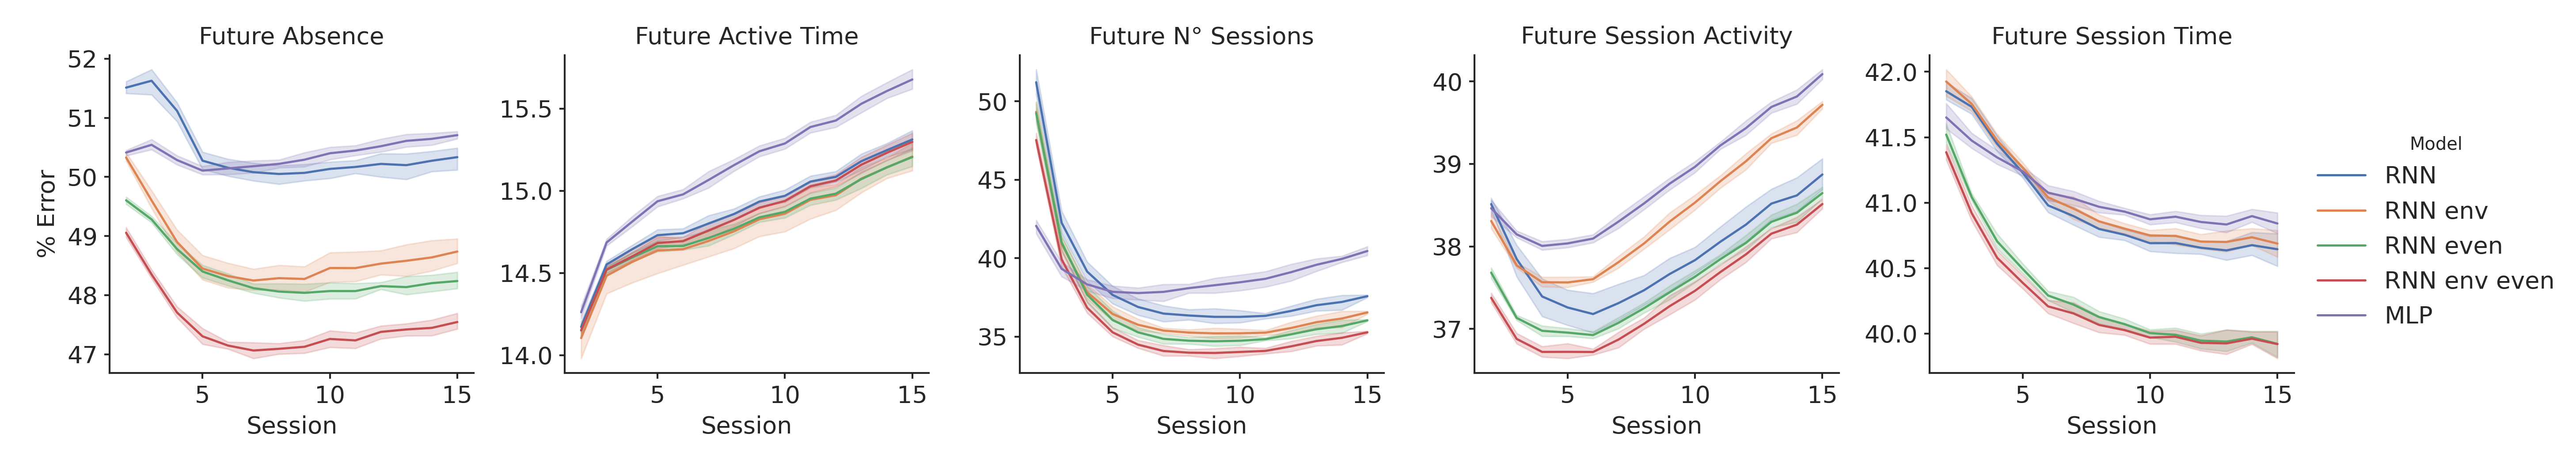
\includegraphics[width=\textwidth]{images/chapter_3/models_comparison_collapsed_game_33.png}
\caption[\textbf{Model comparison collapsing over game context}]{ Overall, our approach (RNN) outperforms all the competing approaches at every time horizon. Each column represent the perfromance of the considered models on a specific target. Solid lines indicate the expected \% error over time for a specific combination of target and model. Dashed areas indicate the standard error of the mean.}
\label{model_comp_coll_game_33}
\end{figure}
\lorem
\begin{figure}[h]
\centering
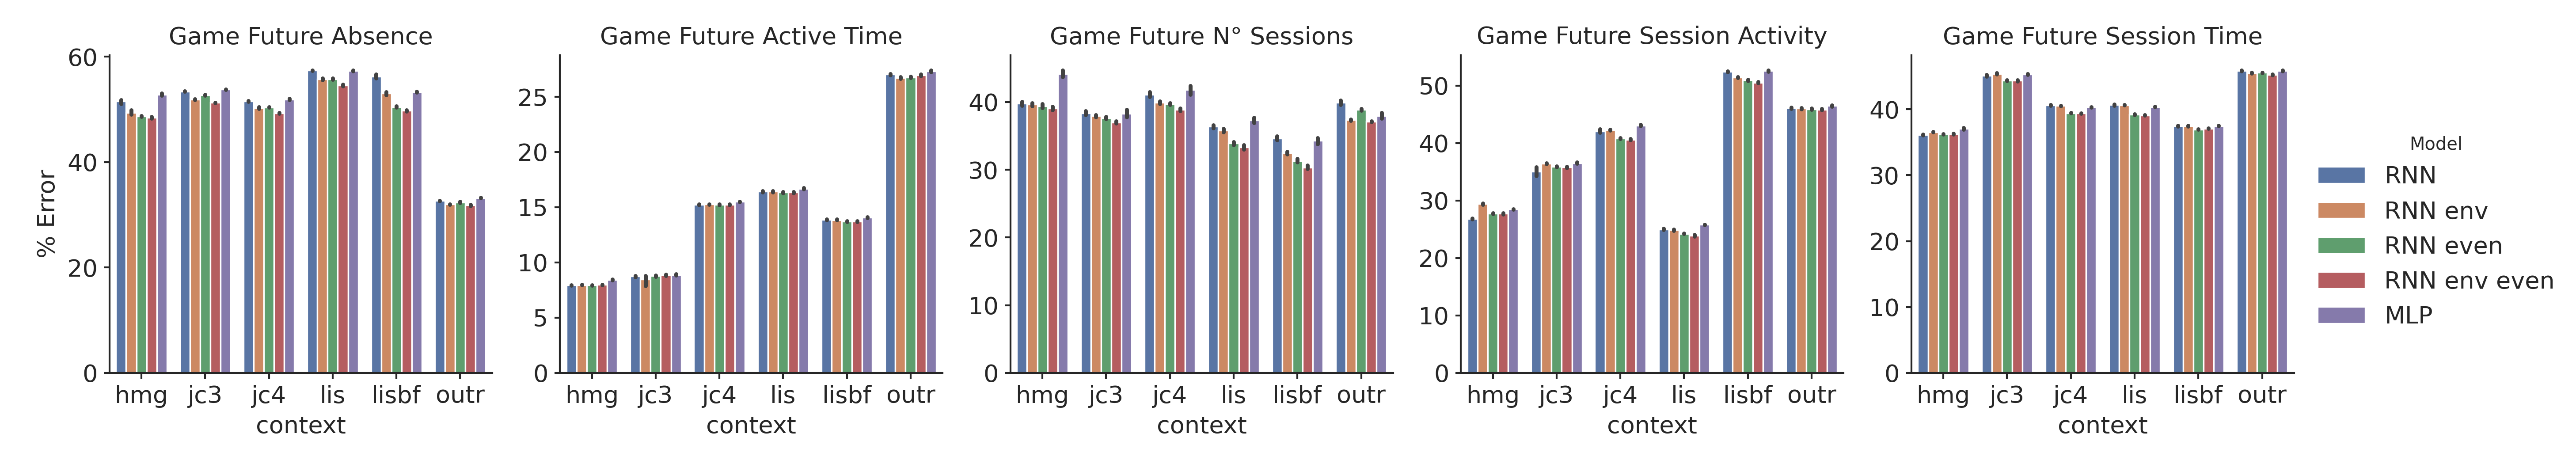
\includegraphics[width=\textwidth]{images/chapter_3/models_comparison_collapsed_time_33.png}
\caption[\textbf{Model comparison collapsing over time}]{ Overall, our approach (RNN) outperforms all the competing approaches in most of the target-game context combinations. Each column represent the perfromance of the considered models on a specific target. Bars indicate the expected \% error for a specific combination of game context, target and model. Black vertical lines indicate the standard error of the mean.}
\label{model_comp_coll_time_33} 
\end{figure}
\lorem
\begin{figure}[h]
\centering
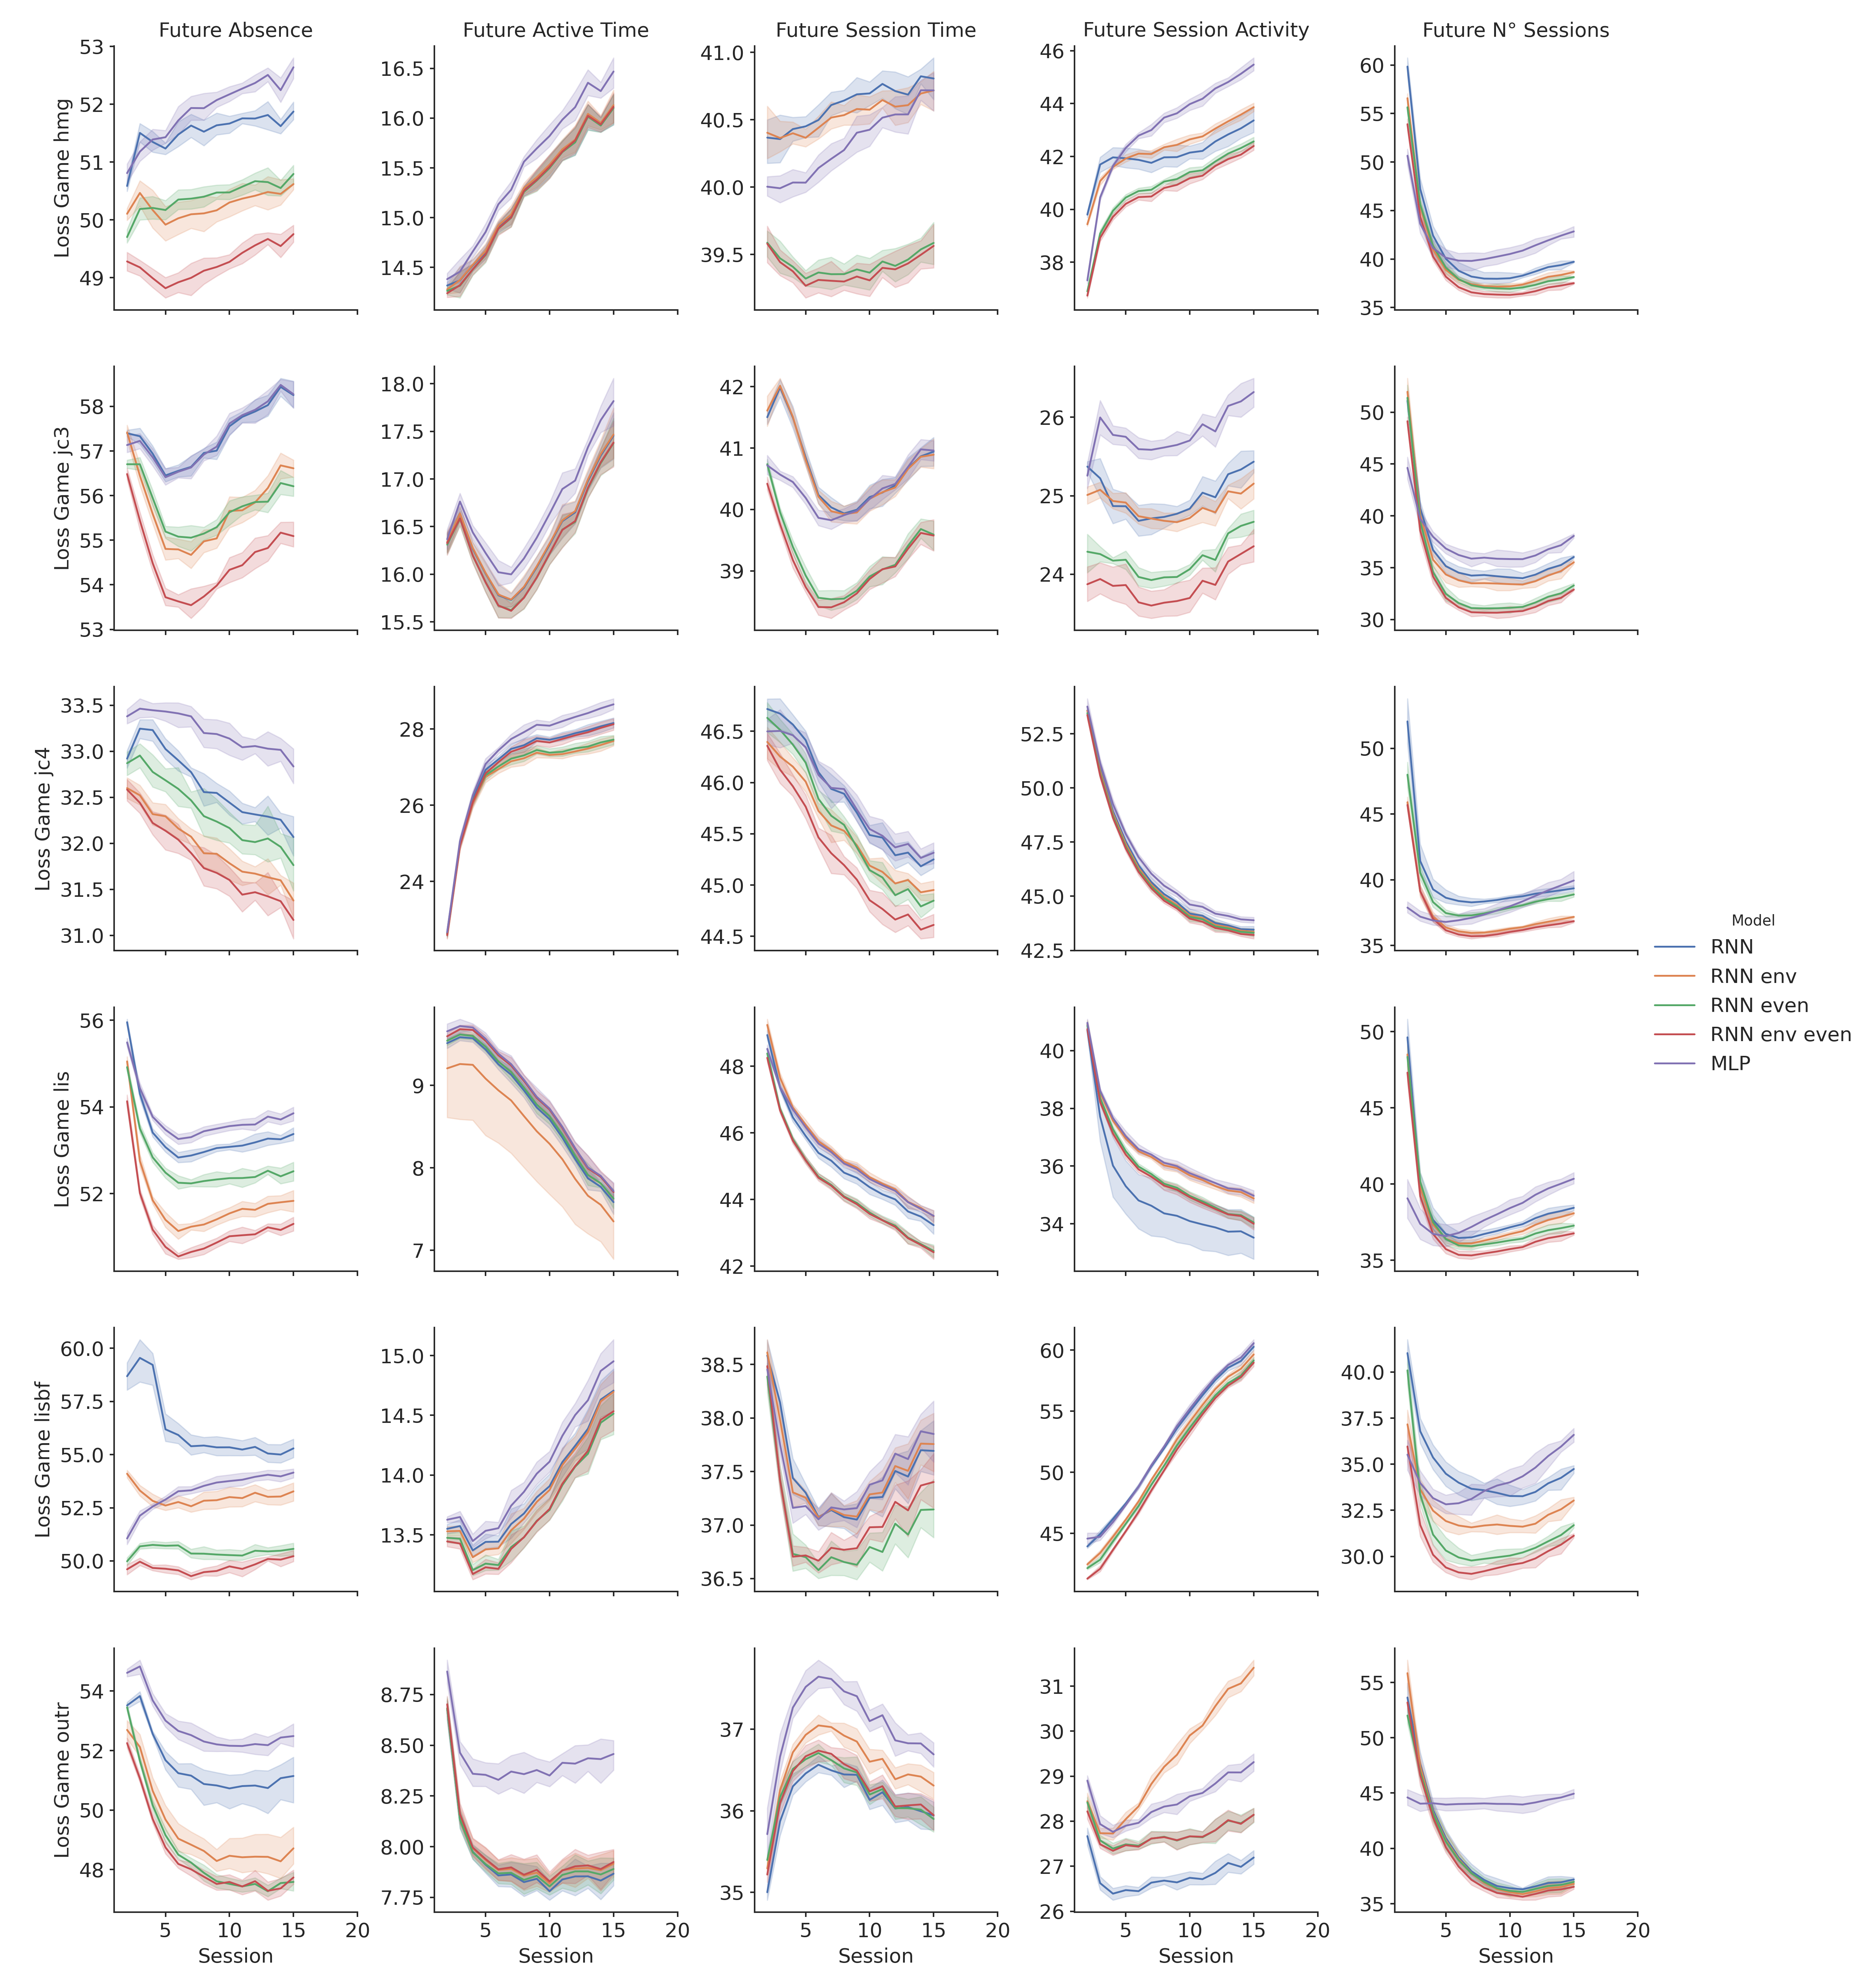
\includegraphics[height=0.5\textheight,keepaspectratio]{images/chapter_3/models_comparison_non_collapsed_33.png}
\caption[\textbf{Model comparison without collapsing}]{ Overall, our approach (RNN) outperforms all the competing approaches in most of the target-game context combinations and temporal horizons. Each column represents the perfromance of the considered models on a specific target while each row reports the perfromance on a specific game context. Solid lines indicate the expected \% error over time for a specific combination of target and model. Dashed areas indicate the standard error of the mean.}
\label{model_comp_non_coll_33} 
\end{figure}
\lorem
\begin{figure}[h]
\centering
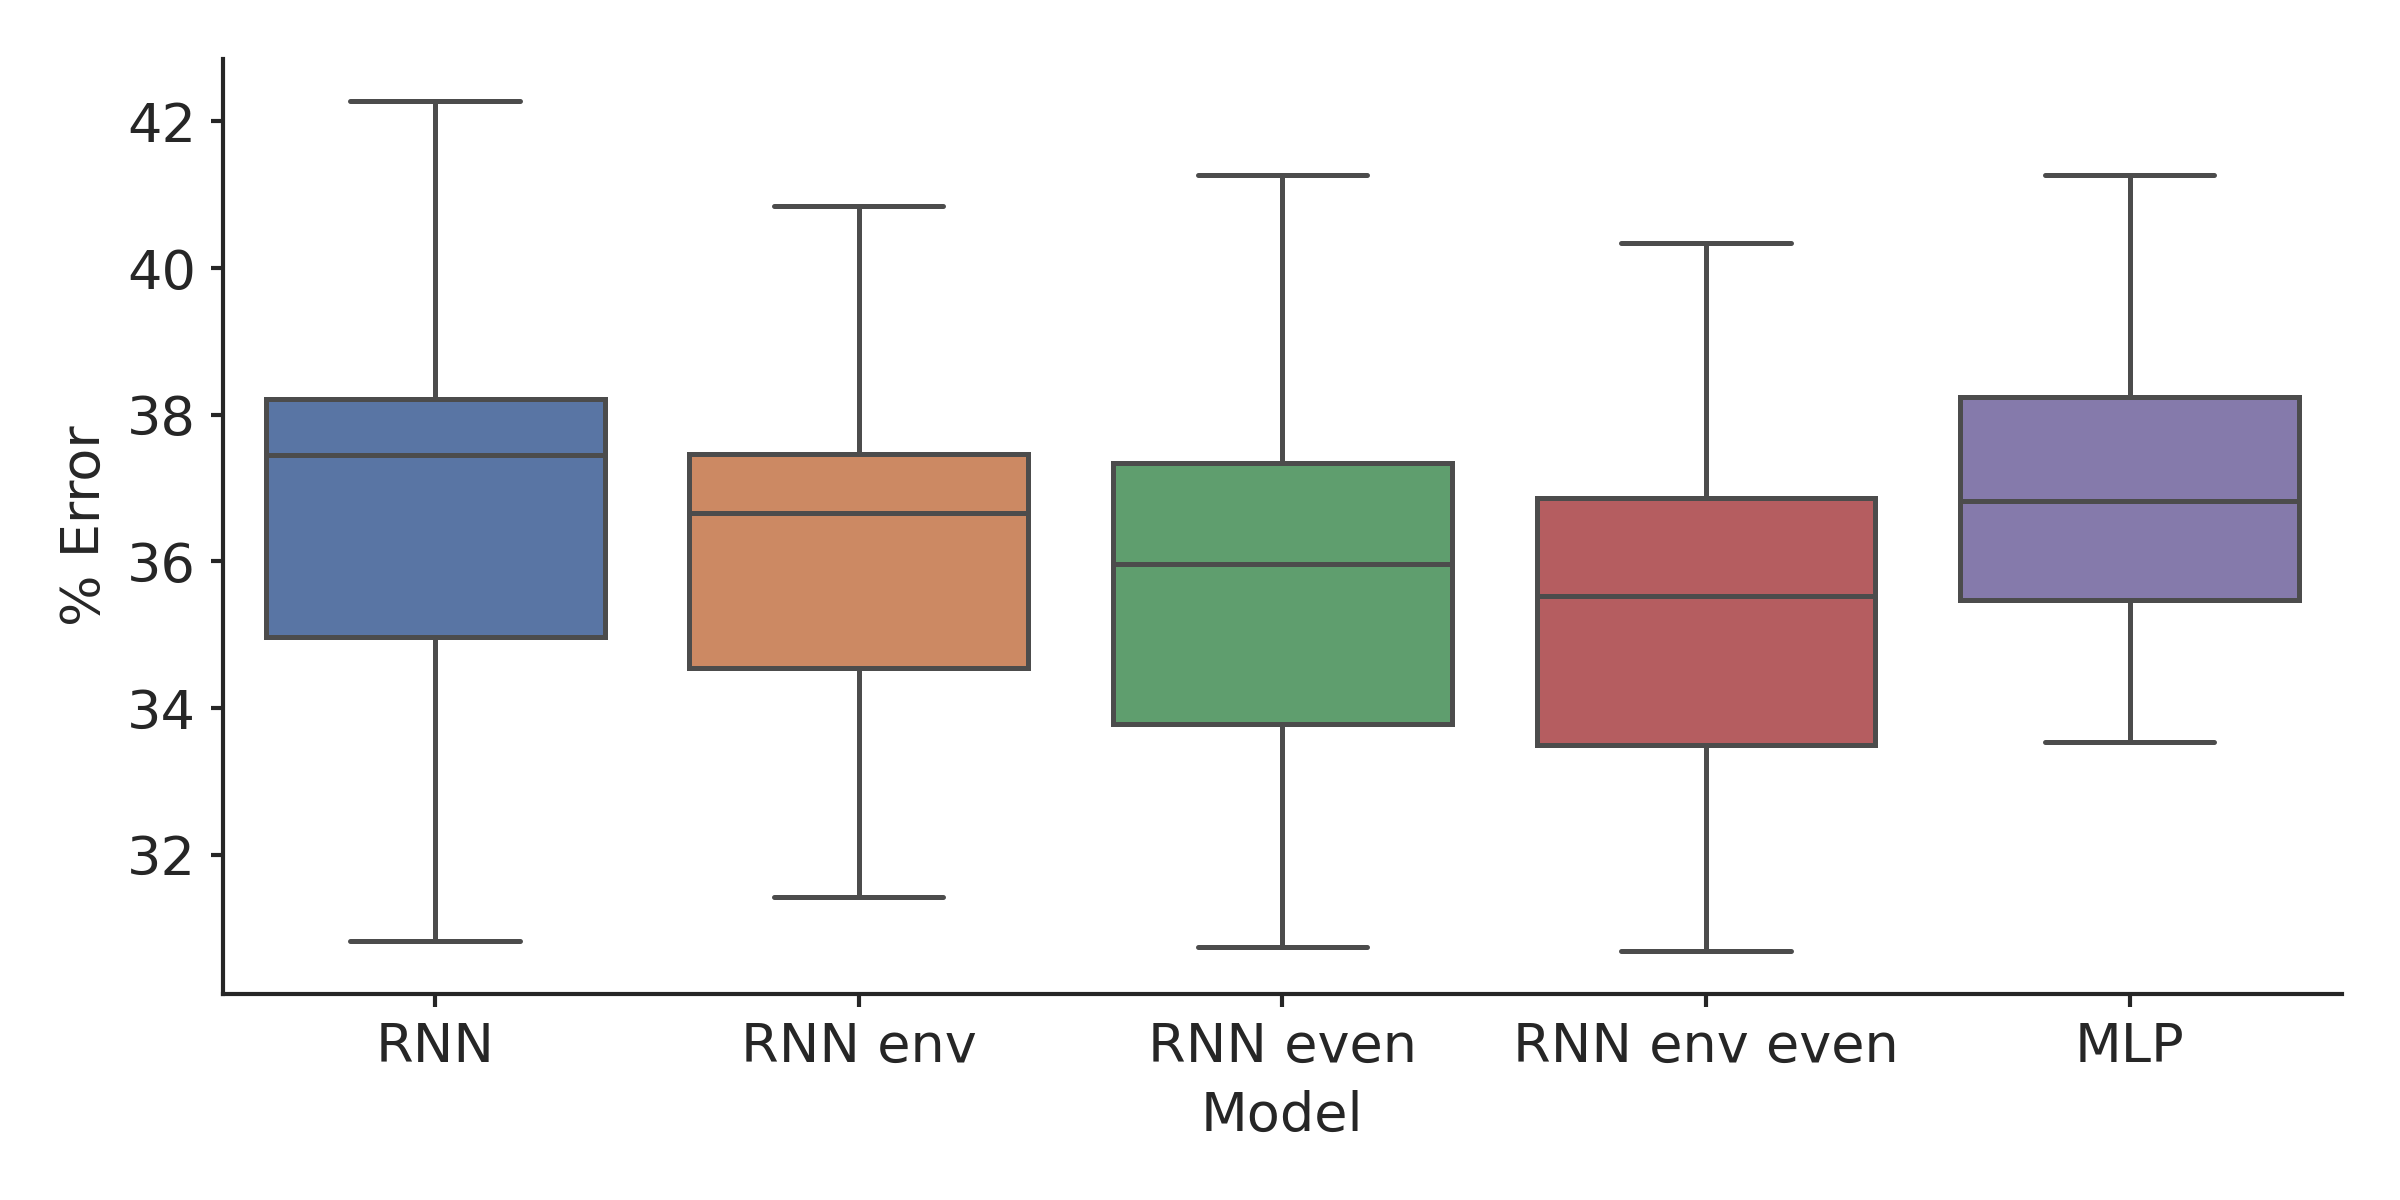
\includegraphics[width=.5\columnwidth]{images/chapter_3/performance_collapsed_33.png}
\caption[\textbf{Aggregated comparison of model performance}]{ Overall, our approach (RNN) outperforms all the competing approaches. Box-plots show the 10-fold cross-validation performance expressed as the total percentage of error (i.e. SMAPE) of each model over the five targets.}
\label{model_comp_coll_33} 
\end{figure}
\lorem
\begin{table}[h]
\centering
\caption{Results of LMM on Collapsed Targets (Sum)}
\label{collapsed_lmm_33}
\begin{tabular}{ccccc}
\hline
\textbf{Model}           & \textbf{$\beta$} & \textbf{Z} & \textbf{p} & \textbf{95\% C.I.} \\ \hline
\multicolumn{5}{c}{\textbf{Collapsed Targets (Sum)}}                                                 \\ \hline
\textbf{Intercept (RNN)} & 36.518                & 41.374     & \textless .01   & 34.788 - 38.248      \\
\textbf{MLP}           & .366                 & 7.569     & \textless .01   & .271 - .460        \\
\textbf{RNN env}          & -.494                 & -1.224     & \textless .01   & -.589 - -.399        \\
\textbf{RNN even}            & -.938                 & -27.424     & \textless .01   & -1.419 - -1.230        \\
\textbf{RNN env even}             & -1.325                 & -19.414     & \textless .01   & -1.032 - -.843        \\ \hline
\end{tabular}
\end{table}
\begin{table}[h]
\centering
\caption{LMM Post-Hoc on Collapsed Targets (Sum)}
\label{collapsed_post_hoc_33}
\begin{tabular}{ccccc}
\hline
\textbf{Contrast}           & \textbf{$\beta_1$ - $\beta_2$} & \textbf{Z} & \textbf{p} & \textbf{95\% C.I.} \\ \hline
\multicolumn{5}{c}{\textbf{Collapsed Targets (Sum)}}                                                 \\ \hline
\textbf{Lag 1 - Median} & 2.528                & 20.210     & \textless .01   & 2.283 - 2.773      \\
\textbf{Median - ENet}          & 3.292                 & 26.322     & \textless .01   & 3.048 - 3.538        \\
\textbf{ENet - MLP}          & 2.778                 & 22.211     & \textless .01   & 2.533 - 3.024        \\ \hline
\end{tabular}
\end{table}
\lorem
\begin{table}[h]
\centering
\caption{Results of LMM on Non-Collapsed Targets}
\label{exploded_lmm_33}
\begin{tabular}{ccccc}
\hline
\textbf{Model}  & \textbf{$\beta$} & \textbf{Z} & \textbf{p} & \textbf{95\% C.I.}                  \\ \hline

\multicolumn{5}{c}{\textbf{Future Absence}}                                                                         \\ \hline
\textbf{Intercept (RNN)} & 50.44                & 42.24     & \textless .01   & 48.10 - 52.78                     \\
\textbf{MLP}           & -.050                & -.845     & .398   & -.16 - .06                     \\
\textbf{RNN env}          & -1.74                & -29.30     & \textless .01   & -1.85 - -1.62                     \\
\textbf{RNN even}            & -2.93                & -49.34    & \textless .01   & -3.05 - -2.81                     \\
\textbf{RNN env even}             & -2.05                & -34.60     & \textless .01   & -2.17 - -1.94                       \\ \hline

\multicolumn{5}{c}{\textbf{Future Active Time}}                                                                     \\ \hline
\textbf{Intercept (RNN)} & 14.877                & 14.99      & \textless .01  & 12.93 - 16.82                     \\
\textbf{MLP}           & 0.26               & 6.65    & \textless .01  & .19 - .34                     \\
\textbf{RNN env}          & -.09                & -2.41     & .016  & -.17 - -.01                     \\
\textbf{RNN even}            & -.08                & -2.02     &  .043  & -.16 - -.002                     \\
\textbf{RNN env even}             & -.03                & -0.776      &  .438  & -.111 - .04                     \\ \hline

\multicolumn{5}{c}{\textbf{Future Session Time}}                                                                     \\ \hline
\textbf{Intercept (RNN)} & 40.978                & 77.831     & \textless .01  & 39.94 - 42.01                     \\
\textbf{MLP}            & .08                & 2.19     & .02  & .009 - .16                     \\
\textbf{RNN env}          & .05               & 1.28     & .2  & -.02 - .12                     \\
\textbf{RNN even}            & -.67                & -16.98     & \textless .01  & -.75 - .59                     \\
\textbf{RNN env even}             & -.73                & -18.48      & \textless .01  & -.81 - -.65                     \\ \hline

\multicolumn{5}{c}{\textbf{Future Session Activity}}                                                                 \\ \hline
\textbf{Intercept (RNN)} & 37.91                & 27.24     & \textless .01  & \multicolumn{1}{l}{35.18 - 40.64} \\
\textbf{MLP}            & .910                & 5.93     & \textless .01  & \multicolumn{1}{l}{.61 - 1.21} \\
\textbf{RNN env}          & .49                & 3.25     & \textless .01  & \multicolumn{1}{l}{.19 - .79} \\
\textbf{RNN even}            & -.32                & -2.091     & .03  & \multicolumn{1}{l}{.62 - -.02} \\
\textbf{RNN env even}             & -.51                & -3.35 & \textless .01  & \multicolumn{1}{l}{-.81 - -.21} \\ \hline

\multicolumn{5}{c}{\textbf{Future N° Sessions}}                                                                      \\ \hline
\textbf{Intercept (RNN)} & 38.37                & 73.91     & \textless .01  & 37.35 - 39.39                     \\
\textbf{MLP}            & .61                & 5.13     & \textless .01  & .37 - .84                     \\
\textbf{RNN env}          &  -1.17              & -9.89     & \textless .01  & -1.41 - -.94                     \\
\textbf{RNN even}            & -1.55                & -13.05     & \textless .01  & -1.78 - -1.32                     \\
\textbf{RNN env even}             & -2.41                & -20.24      & \textless .01  & -2.64 - -2.17                       \\ \hline
\end{tabular}
\end{table}
\begin{table}[h]
\centering
\caption{LMM Post-Hoc on Non-Collapsed Targets}
\label{exploded_post_hoc_33}
\begin{tabular}{ccccc}
\hline
\textbf{Contrast}  & \textbf{$\beta_1$-$\beta_2$} & \textbf{Z} & \textbf{p} & \textbf{95\% C.I.}                  \\ \hline
\multicolumn{5}{c}{\textbf{Future Absence}}                                                                         \\ \hline
\textbf{MLP - RNN env} & 1.69                & 28.458     & \textless .01   & 1.57 - 1.80                    \\
\textbf{MLP - RNN env even}           & 2.88                & 48.503     & \textless .01   & 2.76 - 3.00                     \\
\textbf{MLP - RNN even}           & 2.00                & 33.759     & \textless .01   &  1.89 - 2.12                     \\
\textbf{RNN env - RNN env even}           & 1.19                & 20.045     & \textless .01   & 1.07 - 1.30                     \\
\textbf{RNN env - RNN even}           & .31                & 5.301     & \textless .01   & .19 - .43                     \\
\textbf{RNN env even - RNN even}          & -.87                & -14.744     & \textless .01   & -.99 - -.76                    \\ \hline

\multicolumn{5}{c}{\textbf{Future Active Time}}                                                                     \\ \hline
\textbf{MLP - RNN env} & 0.36                & -11.305     & \textless .01   & 0.28 - 0.44                     \\
\textbf{MLP - RNN env even}           & 0.3                 & 42.461     & \textless .01   & 0.22 - 0.38                     \\
\textbf{MLP - RNN even}           & 0.35                & 42.461     & \textless .01   & 0.27 - 0.43                     \\
\textbf{RNN env - RNN env even}           & -0.06                & 42.461     & .1   & -0.14 - 0.01                     \\
\textbf{RNN env - RNN even}           & -0.01                & 42.461     &  .69   & -0.095 - 0.06                     \\
\textbf{RNN env even - RNN even}          & 0.05                & 6.438     &  .21   & -0.02 - 0.13                    \\ \hline

\multicolumn{5}{c}{\textbf{Future Session Time}}                                                                     \\ \hline
\textbf{MLP - RNN env} & -2.06                & -11.305     & \textless .01   & -2.42 - -1.70                     \\
\textbf{MLP - RNN env even}           & 7.76                & 42.461     & \textless .01   & 7.40 - 8.12                     \\
\textbf{MLP - RNN even}           & 7.76                & 42.461     & \textless .01   & 7.40 - 8.12                     \\
\textbf{RNN env - RNN env even}           & 7.76                & 42.461     & \textless .01   & 7.40 - 8.12                     \\
\textbf{RNN env - RNN even}           & 7.76                & 42.461     & \textless .01   & 7.40 - 8.12                     \\
\textbf{RNN env even - RNN even}          & 1.17                & 6.438     & \textless .01   & .81 - 1.535                    \\ \hline

\multicolumn{5}{c}{\textbf{Future Session Activity}}                                                                 \\ \hline
\textbf{MLP - RNN env} & -2.06                & -11.305     & \textless .01   & -2.42 - -1.70                     \\
\textbf{MLP - RNN env even}           & 7.76                & 42.461     & \textless .01   & 7.40 - 8.12                     \\
\textbf{MLP - RNN even}           & 7.76                & 42.461     & \textless .01   & 7.40 - 8.12                     \\
\textbf{RNN env - RNN env even}           & 7.76                & 42.461     & \textless .01   & 7.40 - 8.12                     \\
\textbf{RNN env - RNN even}           & 7.76                & 42.461     & \textless .01   & 7.40 - 8.12                     \\
\textbf{RNN env even - RNN even}          & 1.17                & 6.438     & \textless .01   & .81 - 1.535                    \\ \hline

\multicolumn{5}{c}{\textbf{Future N° Sessions}}                                                                      \\ \hline
\textbf{MLP - RNN env} & -2.06                & -11.305     & \textless .01   & -2.42 - -1.70                     \\
\textbf{MLP - RNN env even}           & 7.76                & 42.461     & \textless .01   & 7.40 - 8.12                     \\
\textbf{MLP - RNN even}           & 7.76                & 42.461     & \textless .01   & 7.40 - 8.12                     \\
\textbf{RNN env - RNN env even}           & 7.76                & 42.461     & \textless .01   & 7.40 - 8.12                     \\
\textbf{RNN env - RNN even}           & 7.76                & 42.461     & \textless .01   & 7.40 - 8.12                     \\
\textbf{RNN env even - RNN even}          & 1.17                & 6.438     & \textless .01   & .81 - 1.535                    \\ \hline

\end{tabular}
\end{table}
\begin{figure*}[h]
\centering
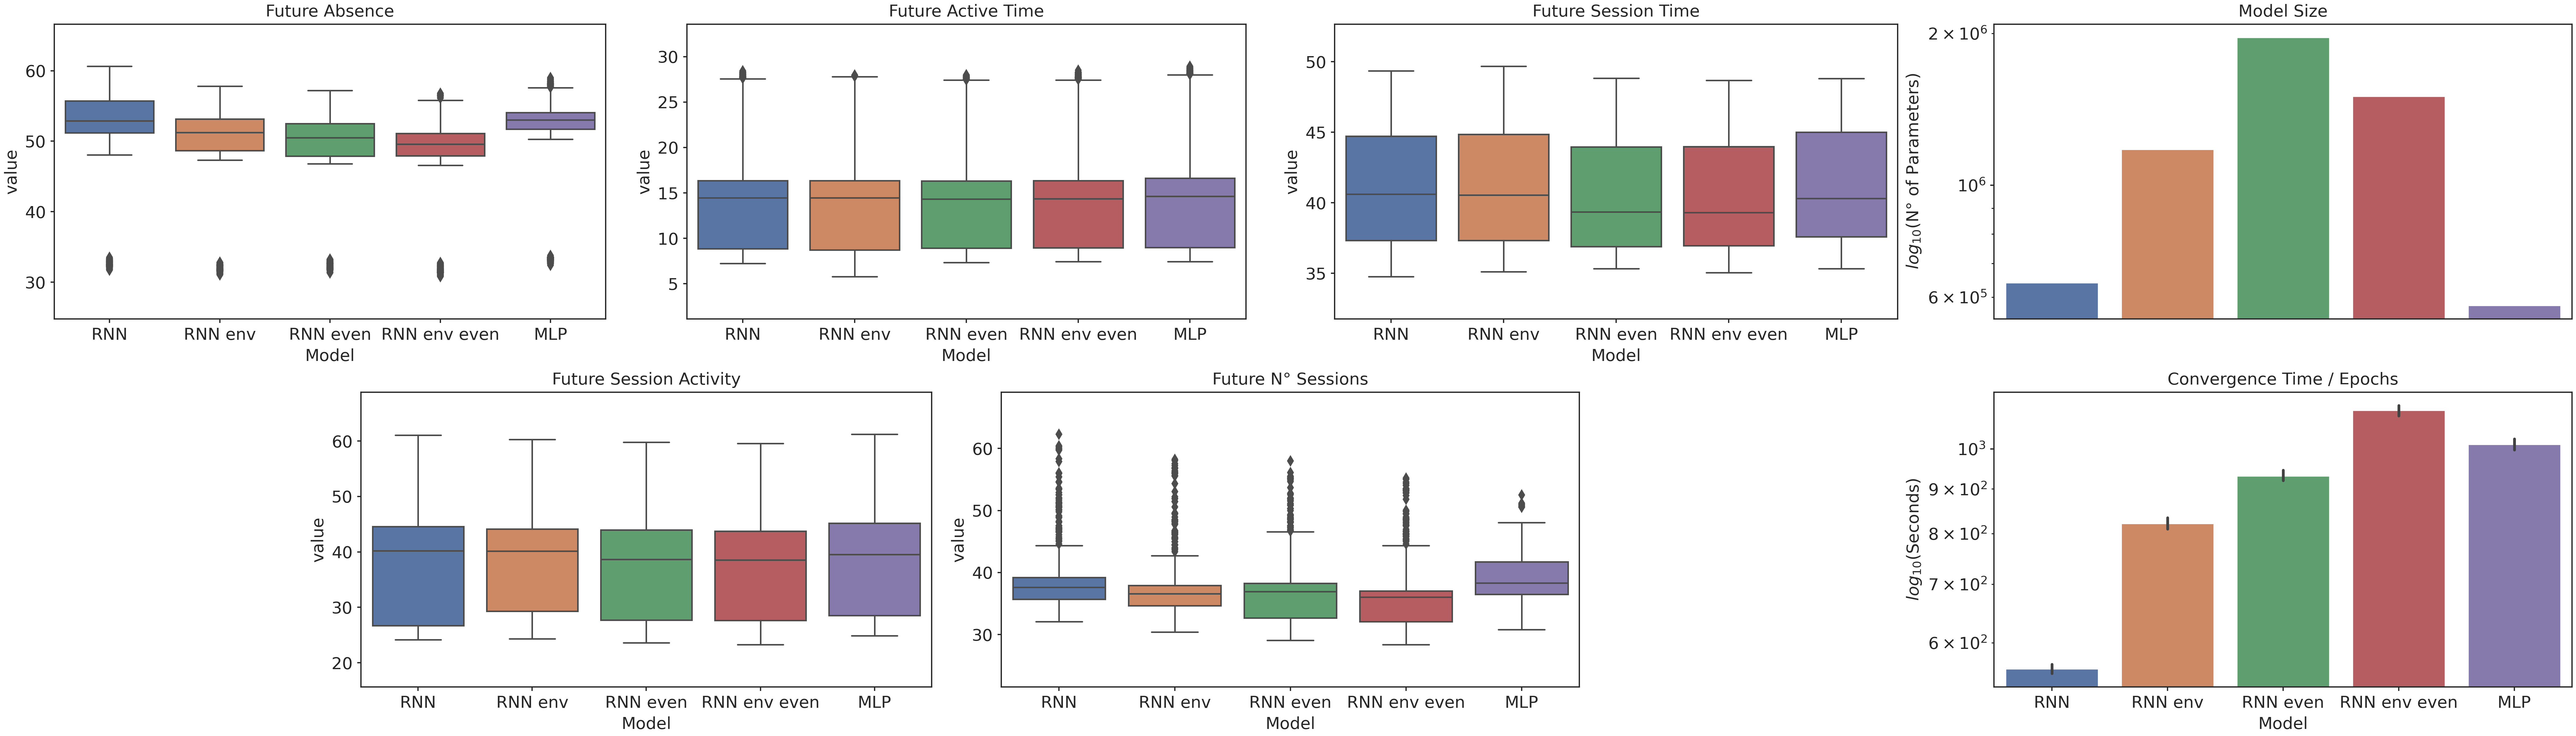
\includegraphics[width=.8\textwidth]{images/chapter_3/performance_exploded_33.png}
\caption[\textbf{Dis-aggregated comparison of models' performance}]{Our approach (RNN) outperformed all competing ones on each target. It consistently used fewer parameters and had shorter computation time than the second best performing model. Box-plots show the 10-fold cross-validation performance expressed as percentage of error (i.e. SMAPE) of each model for the five targets. The bar-plot on the top row indicates the number of free parameters for each model while the bar plot on the bottom row shows the average time for each training epoch. Both bar-plots are $log_{10}$ scaled.}
\label{model_comp_expl_33} 
\end{figure*}

\section{Model Criticism}
\label{model_criticism_3}
The work we just presented is not exempt from limitations. Our approach is formally different from that of TD Learning \footnote{See \cite{barto2004reinforcement} for a  review of the differences between supervised and reinforcement learning.} and does not model the process of incentive salience attribution but rather attempt to approximate the product of this process (i.e. changes in attributed incentive salience). For this reason a direct comparison with the work of McClure \textit{et. al.} \cite{mcclure2003computational} and Zhang \textit{et. al.} \cite{zhang2009neural} is difficult. Moreover, unlike TD learning \cite{schultz1997neural} our model is not guaranteed to converge on a quantification of $V$ that is directly comparable to its biological counterpart or that has arisen from the same type of computations. This is also reinforced by the differences in mechanistic functioning between biological and artificial neural networks \cite{lillicrap2019backpropagation,lillicrap2020backpropagation}. These issues are partially attenuated by the constraints provided by our theoretical framework but in line with similar reports in the literature \cite{calhoun2019unsupervised,wang2018prefrontal} a verification based on controlled experiments is desirable. Differently from the works of Calhoun \textit{et. al.} \cite{calhoun2019unsupervised},  McClure \textit{et. al.} \cite{mcclure2003computational} and Zhang \textit{et. al.} \cite{zhang2009neural}, our methodology relies on a  supervised learning approach to perform both prediction of future behaviour and latent state estimation, making this two tasks infeasible before any data is observed. This limitation could be attenuated by initializing our model using a representation  generated in an unsupervised manner. As we mentioned in section \ref{videogame_telemetries} the reward dynamics generated by the interaction between the individual and the game incentive mechanics play an important role in determining the intensity of future playing behaviour \cite{agarwal2017quitting, avserivskis2017computational, wang2018beyond}. Lastly, despite the fact that our approach appeared to deal gracefully  with objects having different structural characteristics, these were limited to the domain of video games. In order to verify the generalizability of our approach, future work should include data generated from a variety of contexts (e.g. web services, online and laboratory-based experiments).


\section{Discussion}
The advantage provided by the combination of non-linearity and recurrency in the estimation task is in line with the dynamical nature of motivation and incentive salience attribution \cite{toates1994comparing,robinson1993neural,zhang2009neural,tindell2009dynamic,berridge2012prediction}. This is also consistent with a body of research showing that the attribution of value to potentially rewarding objects or actions is often carried out by non-linear recurrent operations \cite{song2017reward,wang2018prefrontal} and that Artificial Neural Networks with recurrent connections are well suited for approximating these operations \cite{kietzmann2018deep}. These findings are corroborated not just by the superior performance of the RNN model in the prediction task (see section \ref{perf_results}) but also by its capacity to produce more stable representations (see Figure \ref{predictive_panel}).
The results of our experiments highlight how employing metrics indicative of behavioural activity in early user-game interactions allowed our model to estimate proxy measures of future disengagement and sustained engagement. This suggests that the early user-game interactions might be relevant for characterizing long-term engagement as well as that measures of behavioural activity could be a useful index for its inference \cite{milovsevic2017early, mirza2013does}.
This is in accordance with the aforementioned theoretical formalization of engagement as a dynamic process rather than a static construct \cite{o2008user}. 
This could indicate that recurrency both improves model fit and allows for more efficient use of the available parameters.
This show how our intuition about the importance of past behavioural intensity information for predicting future intisity is confirmed and how having an architecture able to model dynamical system with memory can help leverage all the historical information. 



\chapter{Representation Analysis}
\label{chapter_repr_anal}
\section{Introduction}
\label{representation_analysis_introduction}
 \footnote{All the code, associated with the work presented in this chapter can be found in the following repositories \begin{itemize}
     \item \href{https://github.com/vb690/approx_incentive_salience}{ApproxIncentiveSalience}
     \item \href{https://github.com/vb690/improved_approx_incentive_salience}{ImprovedApproxIncentiveSalience}
 \end{itemize}}
In this chapter we will analyze the representations inferred by the architectures developed in chapter \ref{chapter_implementation_testing}. Despite the fact that the predictive properties assessed in chapter \ref{chapter_implementation_testing} are a necessary condition for a good approximation of the motivational state of an individual (see section \ref{comp_framework}, they are not sufficient. In this chapter, our aim will be to evaluate if they possess some of the functional characteristics of attributed incentive salience: a true model of physiological motivational state.

In contrast to chapter \ref{chapter_implementation_testing}, we will conduct our investigation using a combination of dimensionality reduction, unsupervised learning and visual analyses. We will focus on evaluating differences and similarities between the representations derived from the RNN architecture and its improved version (i.e., RNN with environmental and game events covariates) as they represent the final versions of our methodology.

We will first briefly introduce the idea that ANNs are able to learn a manifold structure of the data (which reflects the objective function that they are trying to optimize) by embedding it in a high dimensional latent representation. We will also clarify the procedure we followed for extracting these representations using our ANN architectures. Subsequently we will illustrate how it is possible to visualize their manifold structures by means of appropriate dimensionality reduction technique.  After that we will define which type of functional characteristics we expect these structures to show  and which differences we expect to see between the two architectures. Finally by means of unsupervised learning we will conduct a series of exploratory partition analysis on the representations generated by the ANN. This will be done in the attempt to individuate profiles able to map what inferred by the models back to the observable behavioural space. The steps of the analysis pipeline used in this chapter are illustrated in Figure \ref{fig: pipeline_inspect}.
\begin{figure}[!htb]
  \centering
  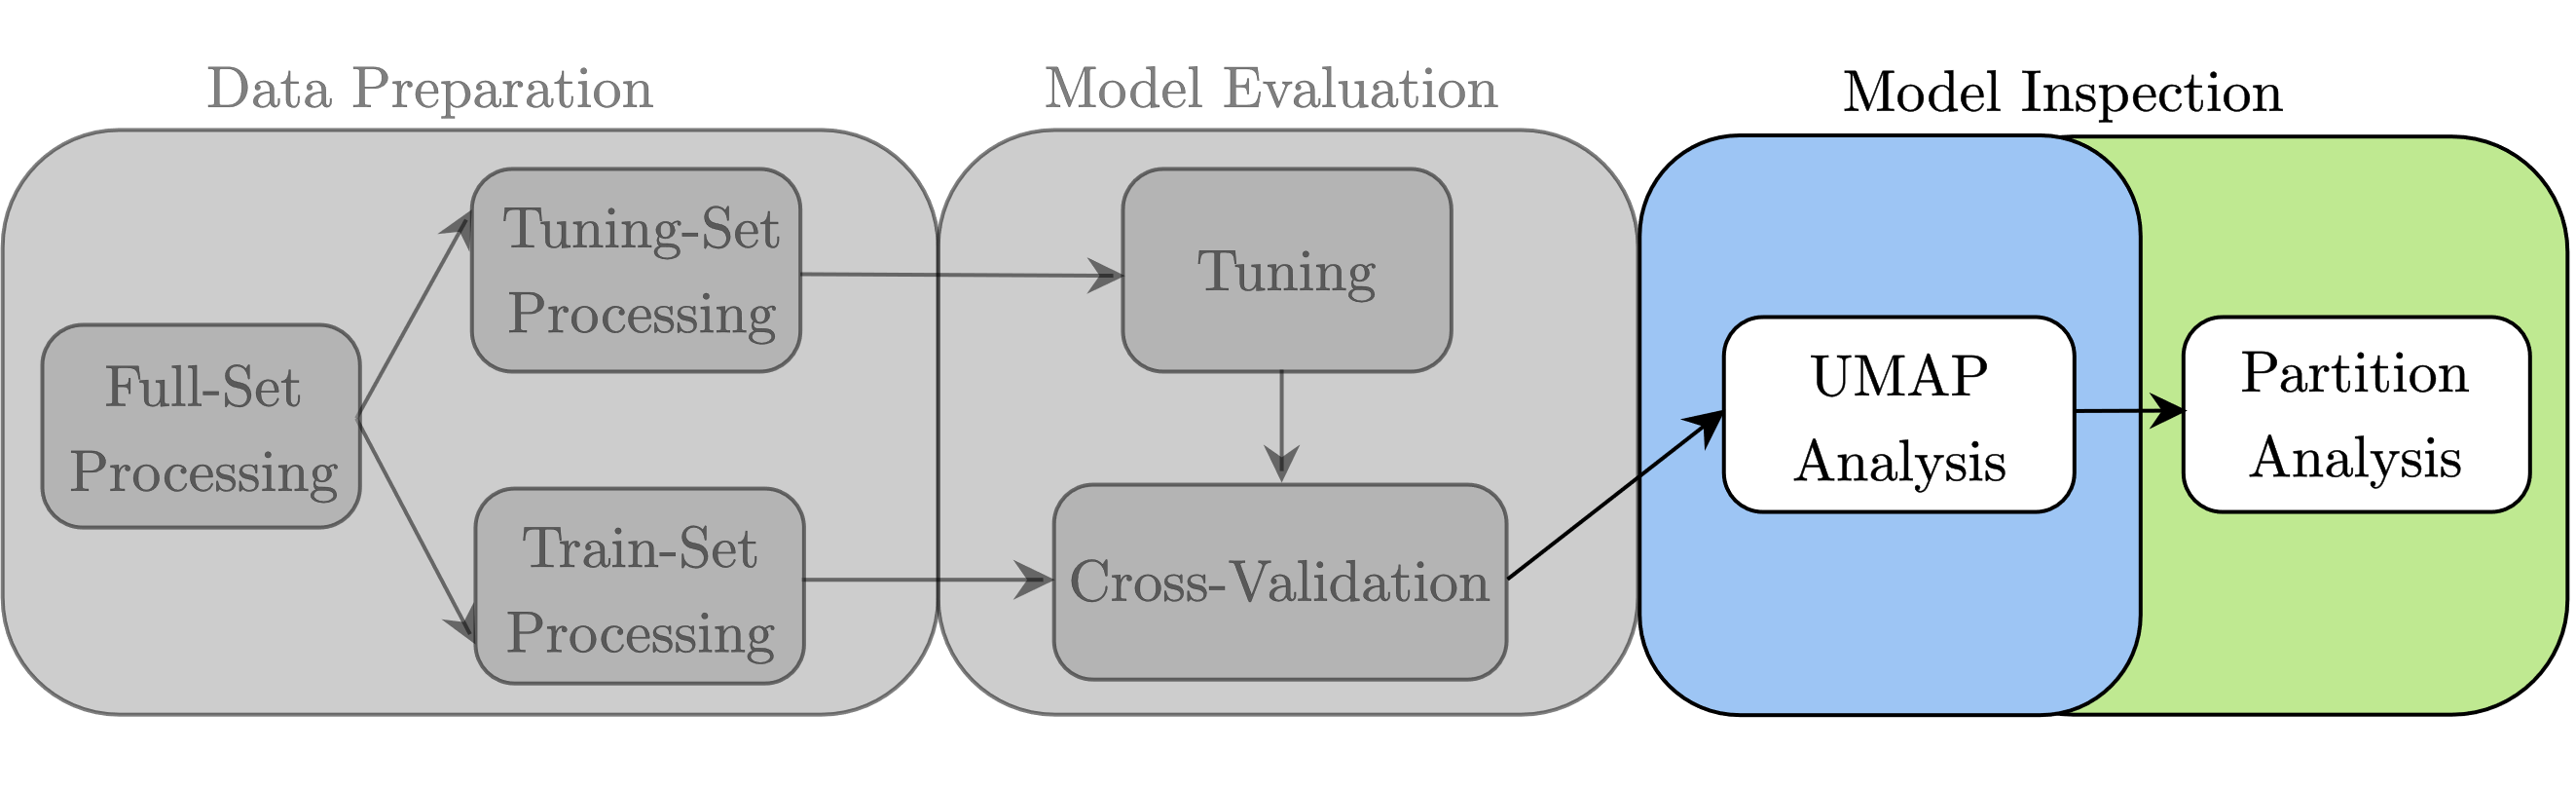
\includegraphics[width=\textwidth]{images/chapter_4/pipeline_inspect.png}
    \caption[\textbf{Representation analysis experimental pipeline}]{Arrows indicate the flow of the pipeline. Big coloured blocks are major pipeline steps, white rectangles indicate sub-tasks within each step. This experimental pipeline stems directly from the "Model Evaluation" stage outline in figure \ref{fig: pipeline_eval}.}
    \label{fig: pipeline_inspect}
\end{figure}

\section{Extracting and Visualizing the Latent Representation}
\label{extract_visulize}

\subsection{Neural Networks, manifolds and embeddings}
\label{manifold_learning_embed}
As we mentioned in section \ref{chapter_theory_modelling}, ANNs approximate a function by mapping the input they receive to a lower dimensional manifold. By moving along this manifold it is possible to reach inputs with different characteristics and observe how they relate with the output produced by the model.

Despite the fact that the manifold structure learned by the model might be intrinsically low dimensional, it is usually stored (or better, it is "embedded"), in a (potentially sparse) high dimensional representation \cite{bengio2017deep}. This representation usually has fewer degrees of freedom than the original input but it is still challenging to parse from a human perspective. Simplifying, this can be compared to storing the "instructions" on how to extract the low dimensional manifold from the input in a distributed fashion across all the parameters of the ANNs. In our case if we look at Figures \ref{fig: rnn_2} and \ref{fig: rnn_env_even}, the portion of the architecture marked in red should, once fitted to the input data, provide us with the relevant "instructions" on how to obtain an approximation of the manifold structure describing the level of attributed incentive salience (see chapter \ref{chapter_theory_modelling} for the theoretical reasons behind this assertion).

As illustrated in sections \ref{artificial_neural_networks} and \ref{manifold_learning}, since an ANNs can be thought as directed acyclic computational graphs (DAGs), to obtain the representation produced at any point of a specific architecture it is sufficient to pass a given input through all the operations performed before that point. Figure \ref{fig: repr_extr} illustrate the process for the RNN architecture presented in section \ref{model_architecture_2}.

\begin{figure}[!htb]
  \centering
  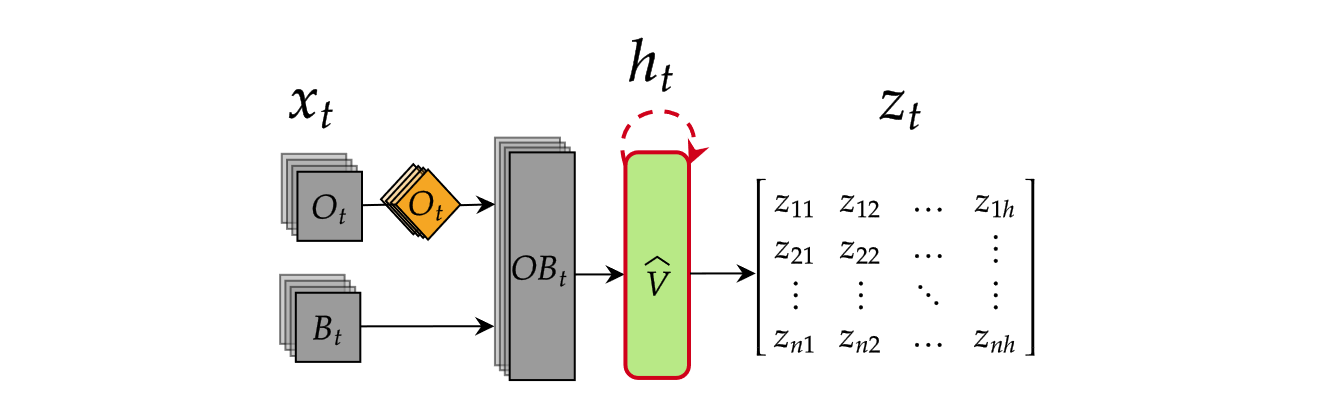
\includegraphics[width=\textwidth]{images/chapter_4/representation_extractor.png}
    \caption[\textbf{The procedure for generating latent representations generated by an ANN}]{Orange and green shapes represent respectively embedding and LSTM layers. Embedding layers are a type of feedforward layers specifically designed for dealing with categorical inputs \cite{chollet2015keras}. Gray shapes indicate operations with no learnable parameters, such as tensor instantiation and concatenation. The orange transparent shape indicate the concatenation of a single embedding with multiple tensors. Stacked, transparent colouring indicates arrays with a sequential structure. Straight and curved arrows refer to the presence of feed-forward or recurrent information flow. The red highlight shows the portion of the model that we hypothesize to be inferring an approximation of attributed incentive salience. Given inputs $O \in \mathbb{Z}^{N \times t}$ and $B \in \mathbb{R}^{N \times t \time 5}$, the matrix $Z_t \in \mathbb{R}^{N \times h}$ represents the $h$ dimensional (where $h$ is the number of hidden units in the recurrent layer) representation generated by the ANN at time $t$ after all operations in its underlying computational graph have been performed.}
    \label{fig: repr_extr}
\end{figure}

Borrowing the terminology from the self-supervised deep learning literature \cite{bengio2017deep} we call this truncated version of the original architecture encoder. Encoders can be thought as functions (whose parameters have been learned during the fitting procedure) mapping input data onto the manifold space learned by the original architecture. From now on, we will use the term encoder for referring to the two considered architectures truncated at the point of the last shared recurrent operation.

\subsection{Dimensionality Reduction and Manifold Approximation}
\label{dim_reduction}
If we look at figure \ref{fig: repr_extr} we can see that with as the size of $h$ increases, it becomes more and more challenging to inspect the representation generated by the encoder. However we recall from section \ref{manifold_learning_embed} that the intrinsic dimensionality for this representation should be much smaller. In the case of a latent state like attributed incentive salience this could be as small as one dimensional, or two if we consider the nature of the rewarding object (see section \ref{motivation_hist} and Figure \ref{fig: vect_mot} in particular). 

A convenient approach for inspecting the shape of this learned manifold would be to peform some form of dimensionality reduction. Principal Component Analysis (PCA) \cite{pearson1901liii} would be a reasonable approach given the straightforward interpretation of the derived components. However the choice of which algorithm to chose is not necessarily that straightforward. 

Looking at figure \ref{fig: swiss_ambient}, we can see the example of a dataset constituted by three separate (the separation aspect is important and will be further in section \ref{functional_properties}) point clouds (denoted by different colours) in a three dimensional ambient space (the space in which a low dimensional manifold might be embedded). Red and green clouds are examples of the synthetic Swiss Roll dataset \cite{scikit-learn}, while the blue cloud is a simple random projection of a square. Both datasets are basically equivalent (i.e. intrinsically two dimensional with the main dimension highlighted by the colour gradient) but differ in their layout in ambient space: the square is linear while the Swiss roll warps in a non linear fashion.

\begin{figure}[!htb]
  \centering
  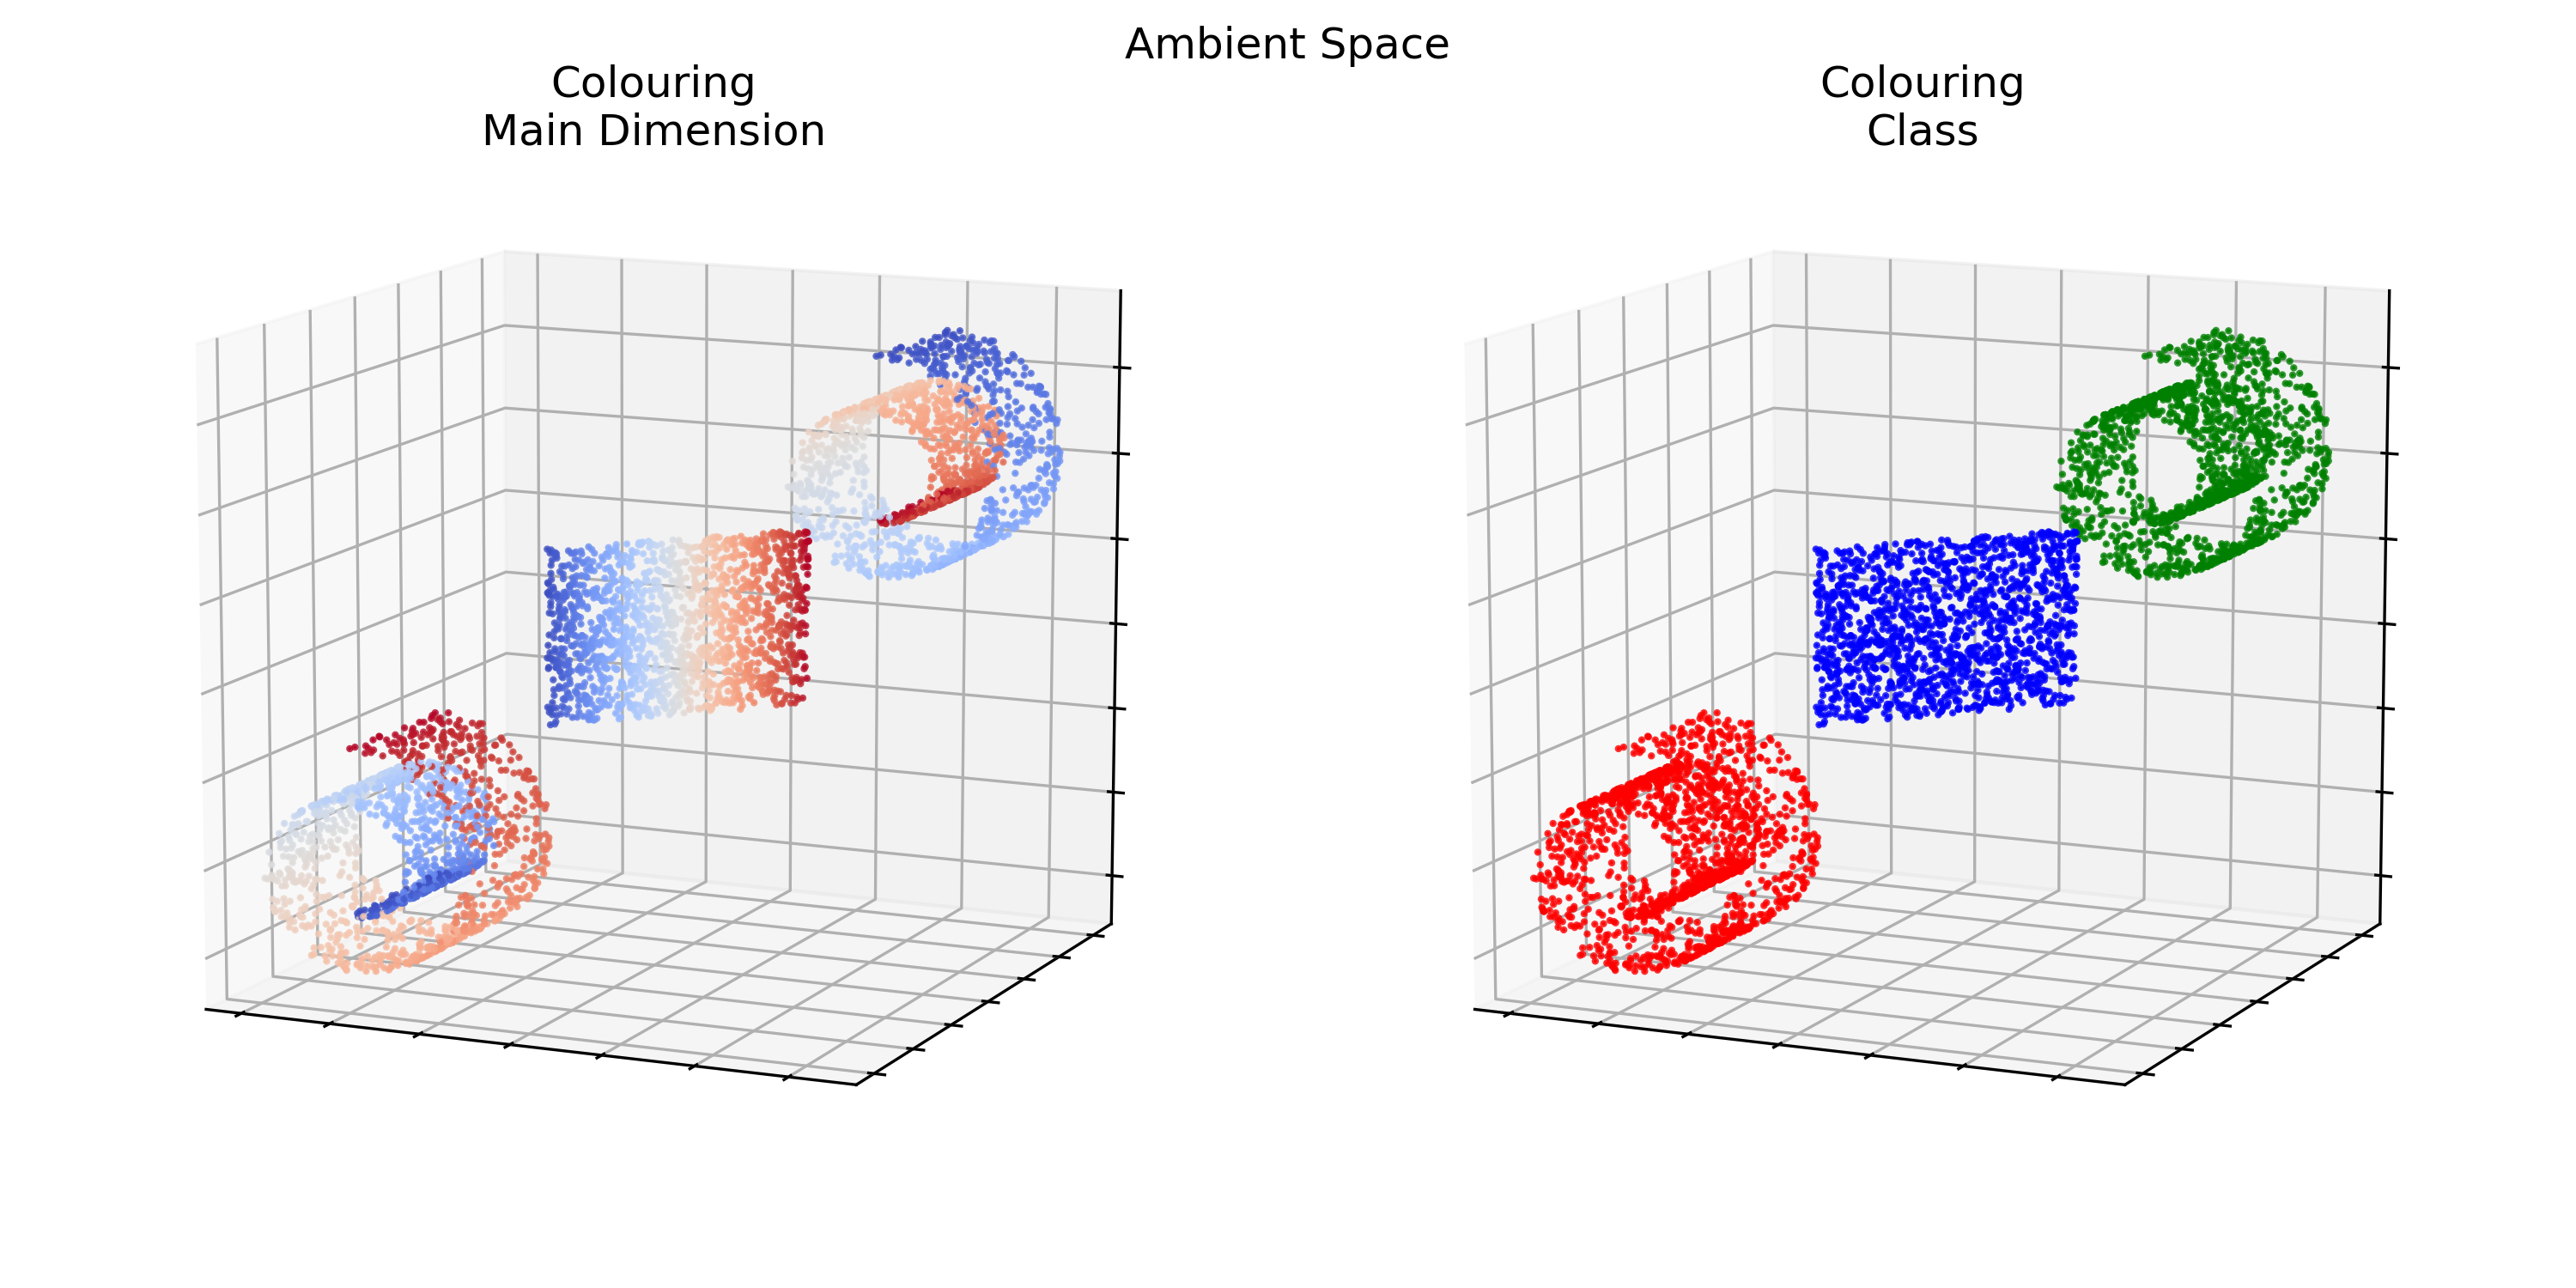
\includegraphics[width=\textwidth]{images/chapter_4/ambient.png}
    \caption[\textbf{Swiss rolls and square in ambient space}]{The figure shows three point clouds which are intrinsically two-dimensional (a Swiss roll and a square) embedded in a three-dimensional ambient space. In both panels the X, y and z axes represent the coordinates of the ambient space. The colours in the first panel indicates the main dimension of variation while those in the second panel simply identify membership of points to a specific cloud.}
    \label{fig: swiss_ambient}
\end{figure}

Figure \ref{fig: swiss_reduce} shows a dimensionality reduction performed by PCA along with an alternative non-linear dimensionality reduction approach: the Uniform Manifold Approximation and Projection (UMAP) \cite{2018arXivUMAP}. 

\begin{figure}[!htb]
  \centering
  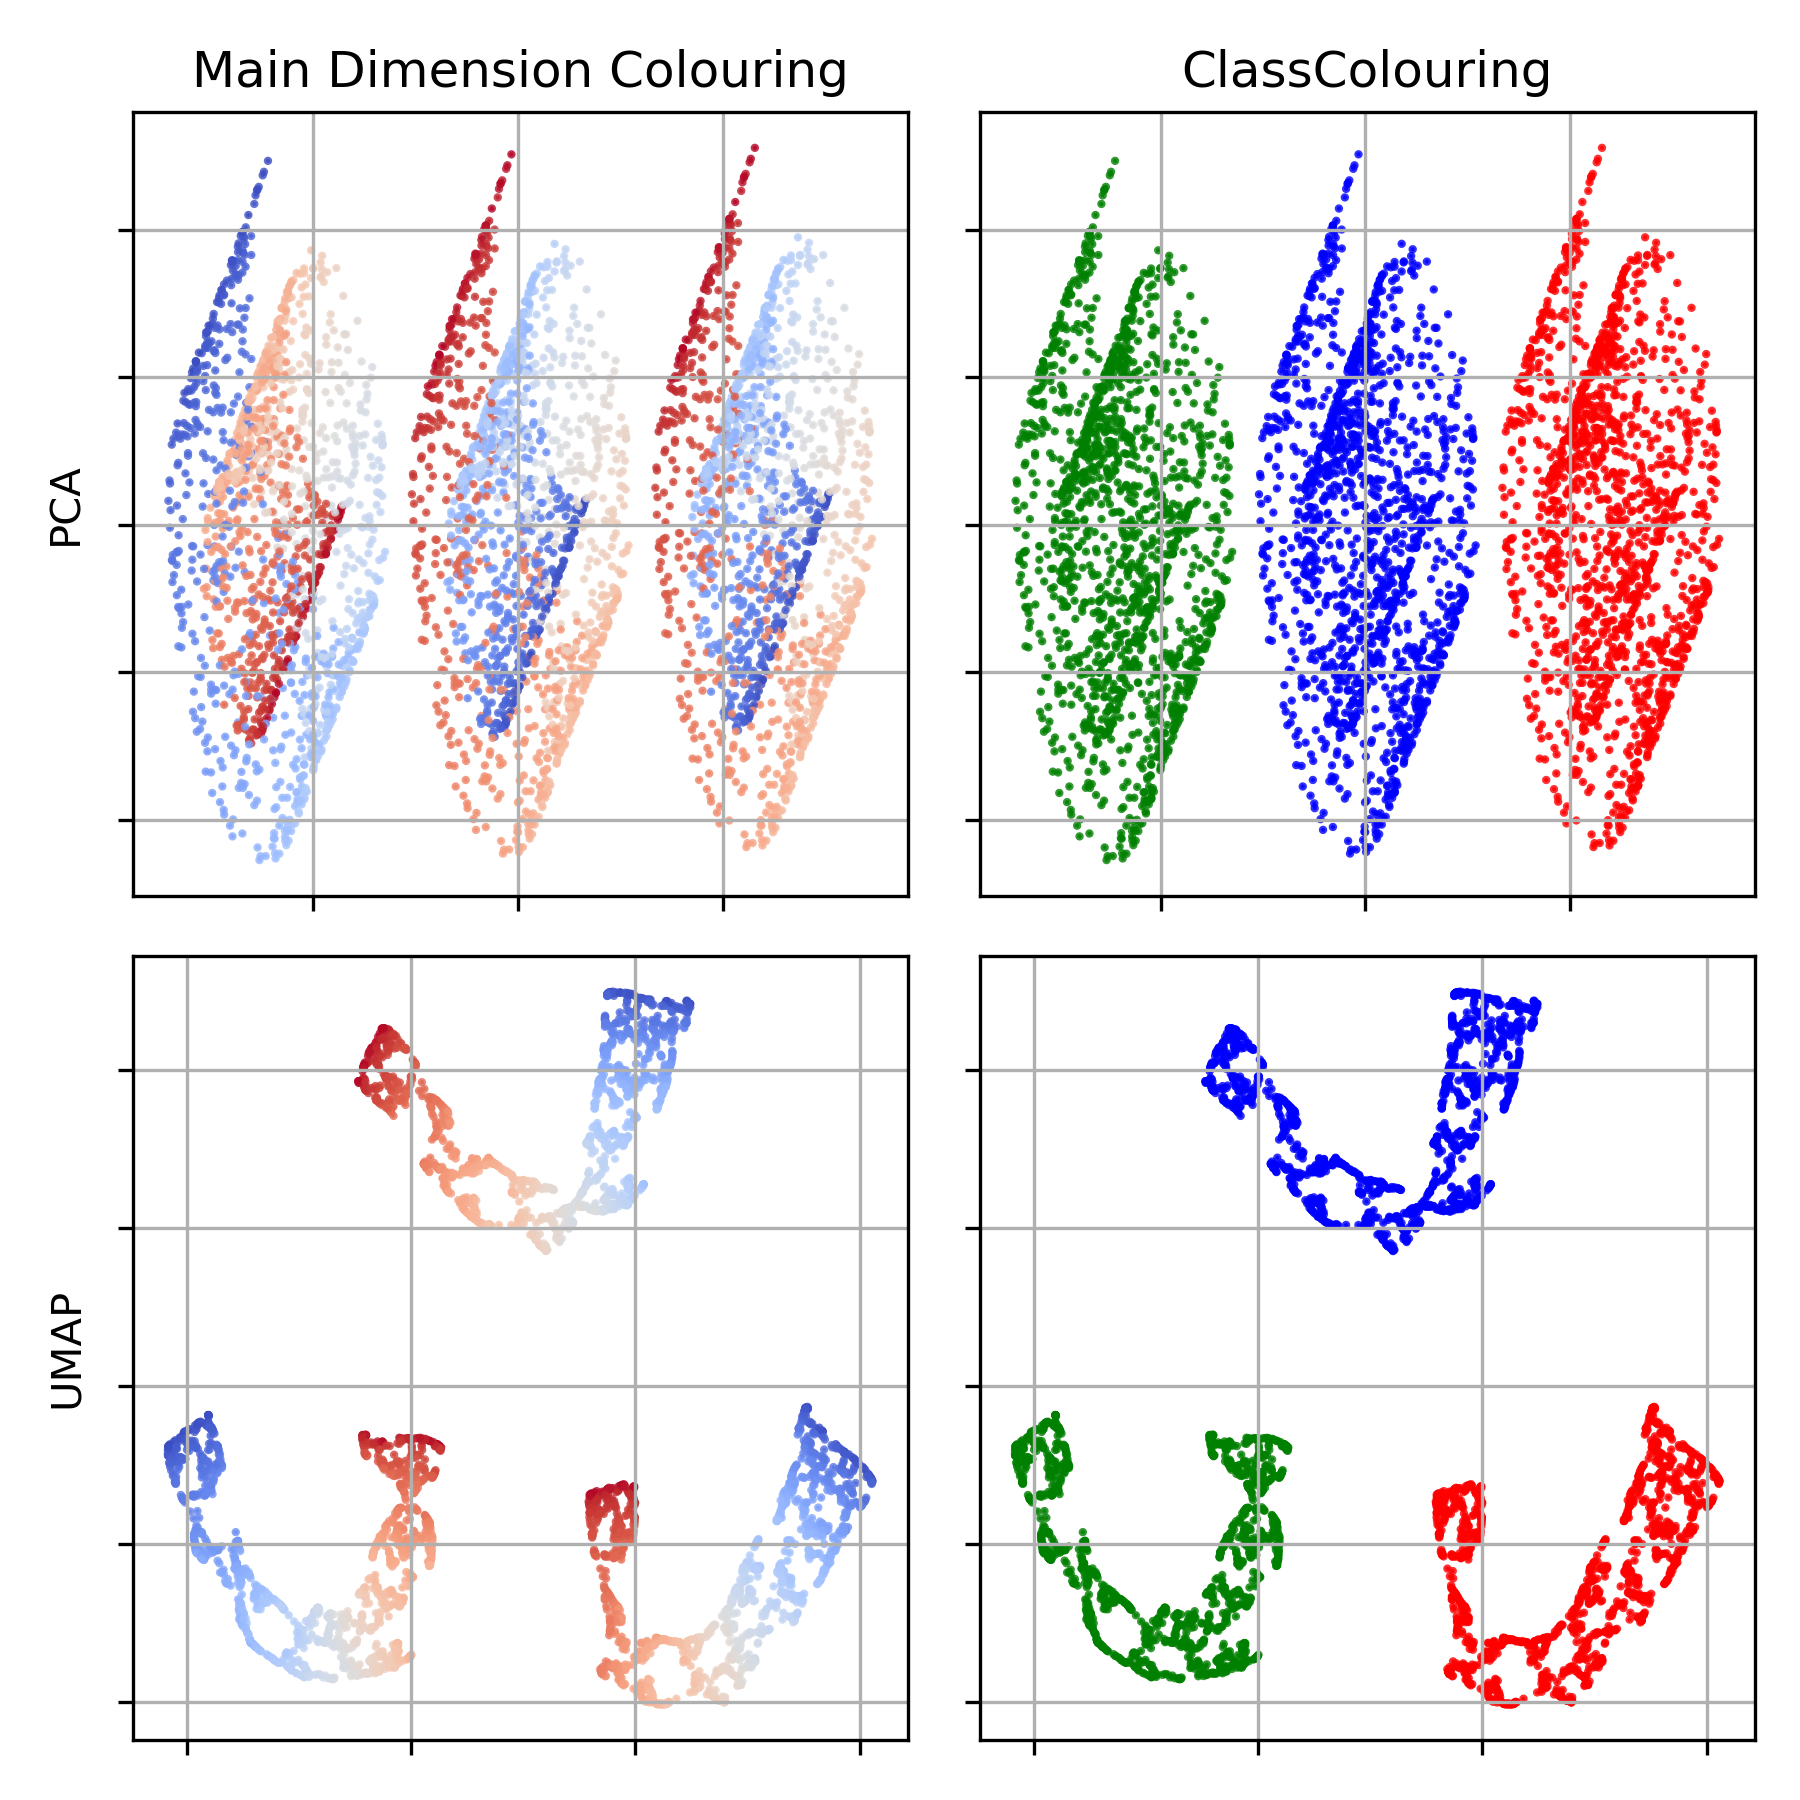
\includegraphics[width=0.7\textwidth]{images/chapter_4/reduced.png}
    \caption[\textbf{PCA and UMAP reduction of Swiss roll and square}]{The figure show the reduction of the three-dimensional point clouds to a two-dimensional plane. The panels in the first row show the reduction produced by PCA while those in the second row show the reduction produced by UMAP. In all panels the x, y axes represent the components extracted by PCA and UMAP. The colours in the two columns again indicate the main dimension of variation and the membership of points to a specific cloud.}
    \label{fig: swiss_reduce}
\end{figure}

The UMAP algorithm is a dimensionality reduction technique based on manifold learning. Given a high dimensional dataset, UMAP first infers its topological structure by means of a k-nearest neighbours graph and then, using stochastic gradient descent, attempts to structurally reproduce it in a lower dimensional space (two or three for visualization purposes) \cite{2018arXivUMAP}. Despite being a local algorithm, compared to other similar approaches (for example, the t-distributed Stochastic Neighbor Embedding \cite{van2008visualizing}),  UMAP has the ability to better preserve the global structure of the original data. Moreover, when given datasets that are sequential in natures (like those produce by the recurrent part of our architecture) UMAP is able to include this characteristics during the optimization process \footnote{See \cite{alignedumap} for implementation details.} generating lower dimensional representations that are aligned over time. 

What we observe in Figure  \ref{fig: swiss_reduce} is that both techniques manage to keep the separation between point clouds, but that PCA, unlike  UMAP, struggles to faithfully represent the the intrinsic structure of the data. This toy example is particularly relevant in our case as the representations generated by ANNs are, by design, highly non-linear. This will be made evident in the next section where we will proceed at visualizing the representation learned by our ANNs architecture.

\section{Representation Analysis}
\label{representation_analysis}
In order to support our idea that the representation learned by the different architectures could be interpreted as an approximation of the latent states generated by incentive salience, we carried out a series of qualitative analyses. If our intuitions were in the right direction, we expected the representations inferred by the architectures to exhibit a series of characteristics and functional properties:
\begin{enumerate}
    \item To possess an intrinsic dimensionality that is much smaller than the observed one.
    \item To be able to effectively distinguish between different game objects.
    \item To be able to effectively distinguish between individuals based on the expected intensity of their future interactions with the considered game objects.
    \item To be able to show the two aforementioned characteristics consistently over time.
\end{enumerate}

The characteristics mentioned above are concerned with a general validation of the properties of the latent representation for all the considered architectures, however we also wanted to understand if the included covariates altered and improved the generated representation.  We therefore inspected the representation extracted by the encoder derived from the improved version of the RNN architecture. 

The procedure followed for extracting the latent representations was the same for all architectures. First, we re-fitted all models on a random sample (i.e. 90\%) of the validation-set following the same procedures specified in chapter \ref{chapter_implementation_testing}. Then, we created six encoders using the approach illustrated in paragraph \ref{manifold_learning_embed} and Figure \ref{fig: repr_extr}. Two were used for extracting the representations expected to approximate the level of attributed incentive salience (red highlights in Figures \ref{fig: rnn_2} and \ref{fig: rnn_env_even}. One for extracting the same type of representation inferred however by the MLP architecture (this was done for comparative purposes). And three were used for extracting the intermediate representations generated by the improved version of the RNN architecture (i.e. those relative to the behavioural, environmental and game events input). Subsequently, we passed the remaining portion of the validation-set (i.e. 10\%) as an input to the encoders, producing arrays of shape $(N \times T \times h)$ with $N$ being the number of considered individuals, $h$ the number of hidden units in the last layer of the encoder and $T$ the number of observed interactions for the considered individuals. This means that all representations have been generated with out-of-sample data. In our case, since all architectures were of type sequence-to-sequence we were able to investigate not just the properties of the generated representation at specific point in time, but also the dynamics underlying their evolution. 

To summarize, each considered encoder was tasked with generating a high dimensional representation where distance could be interpreted as similarity between individuals with respect to the expected intensity of their future interactions with a specific game object (see the manifold hypothesis of attributed incentive salience presented in paragraph \ref{manifold_rep_incentive_salience}). Dimensionality reduction was then used for approximating the intrinsic manifold structure of these representations on a two dimensional plane in order to allow for qualitative visual analysis. 

The reduction to a 2D plane used the UMAP algorithm. The algorithm first inferred the topological structure of the produced representations by computing the cosine distance in a local neighborhood of 1000 points with a minimum distance of 0.8. The projection on a two dimensional plane was then achieved by running the optimization part of the algorithm for 2000 iterations. The choice of a large neighborhood and minimum distance was made to better capture the global structure of the manifold \footnote{See \cite{umapwebs} for a visualization of the effects of these hyperparameters in UMAP.}. 

In order to gather an understanding on the characteristics of the function used for generating the latent representations, we also conducted a set of purely exploratory investigations of the relationship between hidden units' activation in the recurrent layers and the predictions produced by the model. To quantify the strength of the observed relationship we employed the Maximal Information Coefficient (MIC) \cite{reshef2011detecting}, a measure of mutual information that can quantify both linear and non-linear association between variables. The MIC can assume values between 0 to 1 with 1 corresponding to a perfect association. 

We adopted the implementation of UMAP provided McInnes \textit{et. al.} \cite{mcinnes2018umap-software} while the MIC was computed using the python library minepy \cite{albanese2013minerva}. Visualizations were produced using the python libraries matplotlib \cite{hunter2007matplotlib} and seaborn \cite{waskom2021seaborn}.

\subsection{Validating the Functional Properties of the Inferred Latent Representation}
\label{functional_properties}
We first asked if the assumption about the intrinsic dimensionality of the latent representation was reasonable. Looking at figure \ref{cross_corr_act}

\begin{figure}[!htb]
\centering
\includegraphics[width=0.5\textwidth]{images/chapter_4/corr_matrices.png}
\caption[\textbf{Cross-correlation analysis of the hidden units activation of the RNN architecture}]{Each panel shows the cross correlation between the activity of the RNN's artificial neurons in all the game objects going from $t1$ to $t4$. The y and x axes are symmetrical and identify the RNN artificial neurons while the coloured cells indicate the Spearman's Rho correlation coefficient for the activation of each pair of neurons. White cells represent combinations for which the correlation coefficient was lower than 0.05.}
\label{cross_corr_act} 
\end{figure}

we can observe consistent patterns of cross-correlation for the activity of the hidden units constituting the latent representation, suggesting the presence of redundancy. In order to support this finding and to gain a general sense of the intrinsic dimensionality of the embedded manifold, we conducted a Principal Component Analysis (PCA). Despite PCA and UMAP working under radically different assumptions and mechanisms, we thought this could provide us with a general idea of how much variance we would be able to capture by reducing the representation to a lower dimensional space. 

\begin{figure}[!htb]
\centering
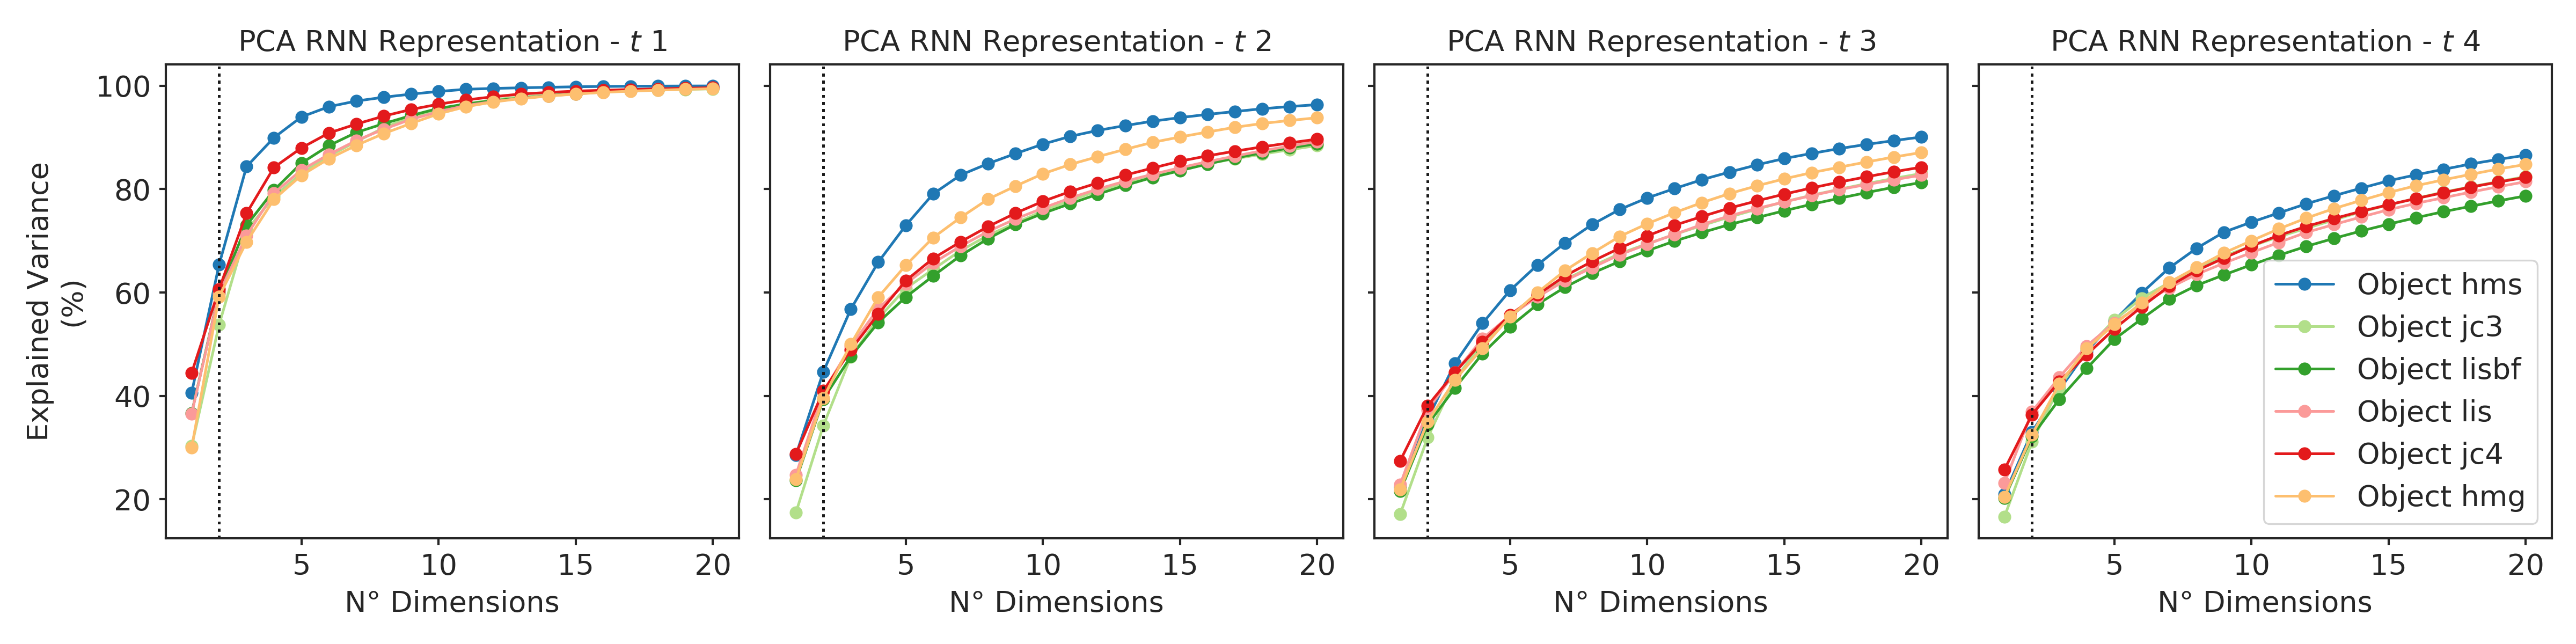
\includegraphics[width=\textwidth]{images/chapter_4/pca_embedding.png}
\caption[\textbf{Principal component analysis of the hidden units activation of the RNN architecture }]{The panel shows the percentage of explained variance by considering 2 to 20 principal components for each game object going from $t1$ to $t4$. The y axis indicates the percentage of explained variance while the x axis the number of principal components considered.}
\label{pca_emb} 
\end{figure}

Looking at figure \ref{pca_emb} we can see that two principal components can explain a large portion of variance in the representation generated by the RNN. To be precise, across game contexts the first two principal components were able to explain from 30 to 60\% of the variance, with maximum explanatory power around 6 and 8 principal components. However, as we illustrated in section \ref{dim_reduction}, relying on PCA alone could give us an incomplete and potentially distorted picture of the manifold structure inferred by the architecture. Looking at Figure \ref{temporal_panel_rnn_pca} 

\begin{figure}[!htb]
\centering
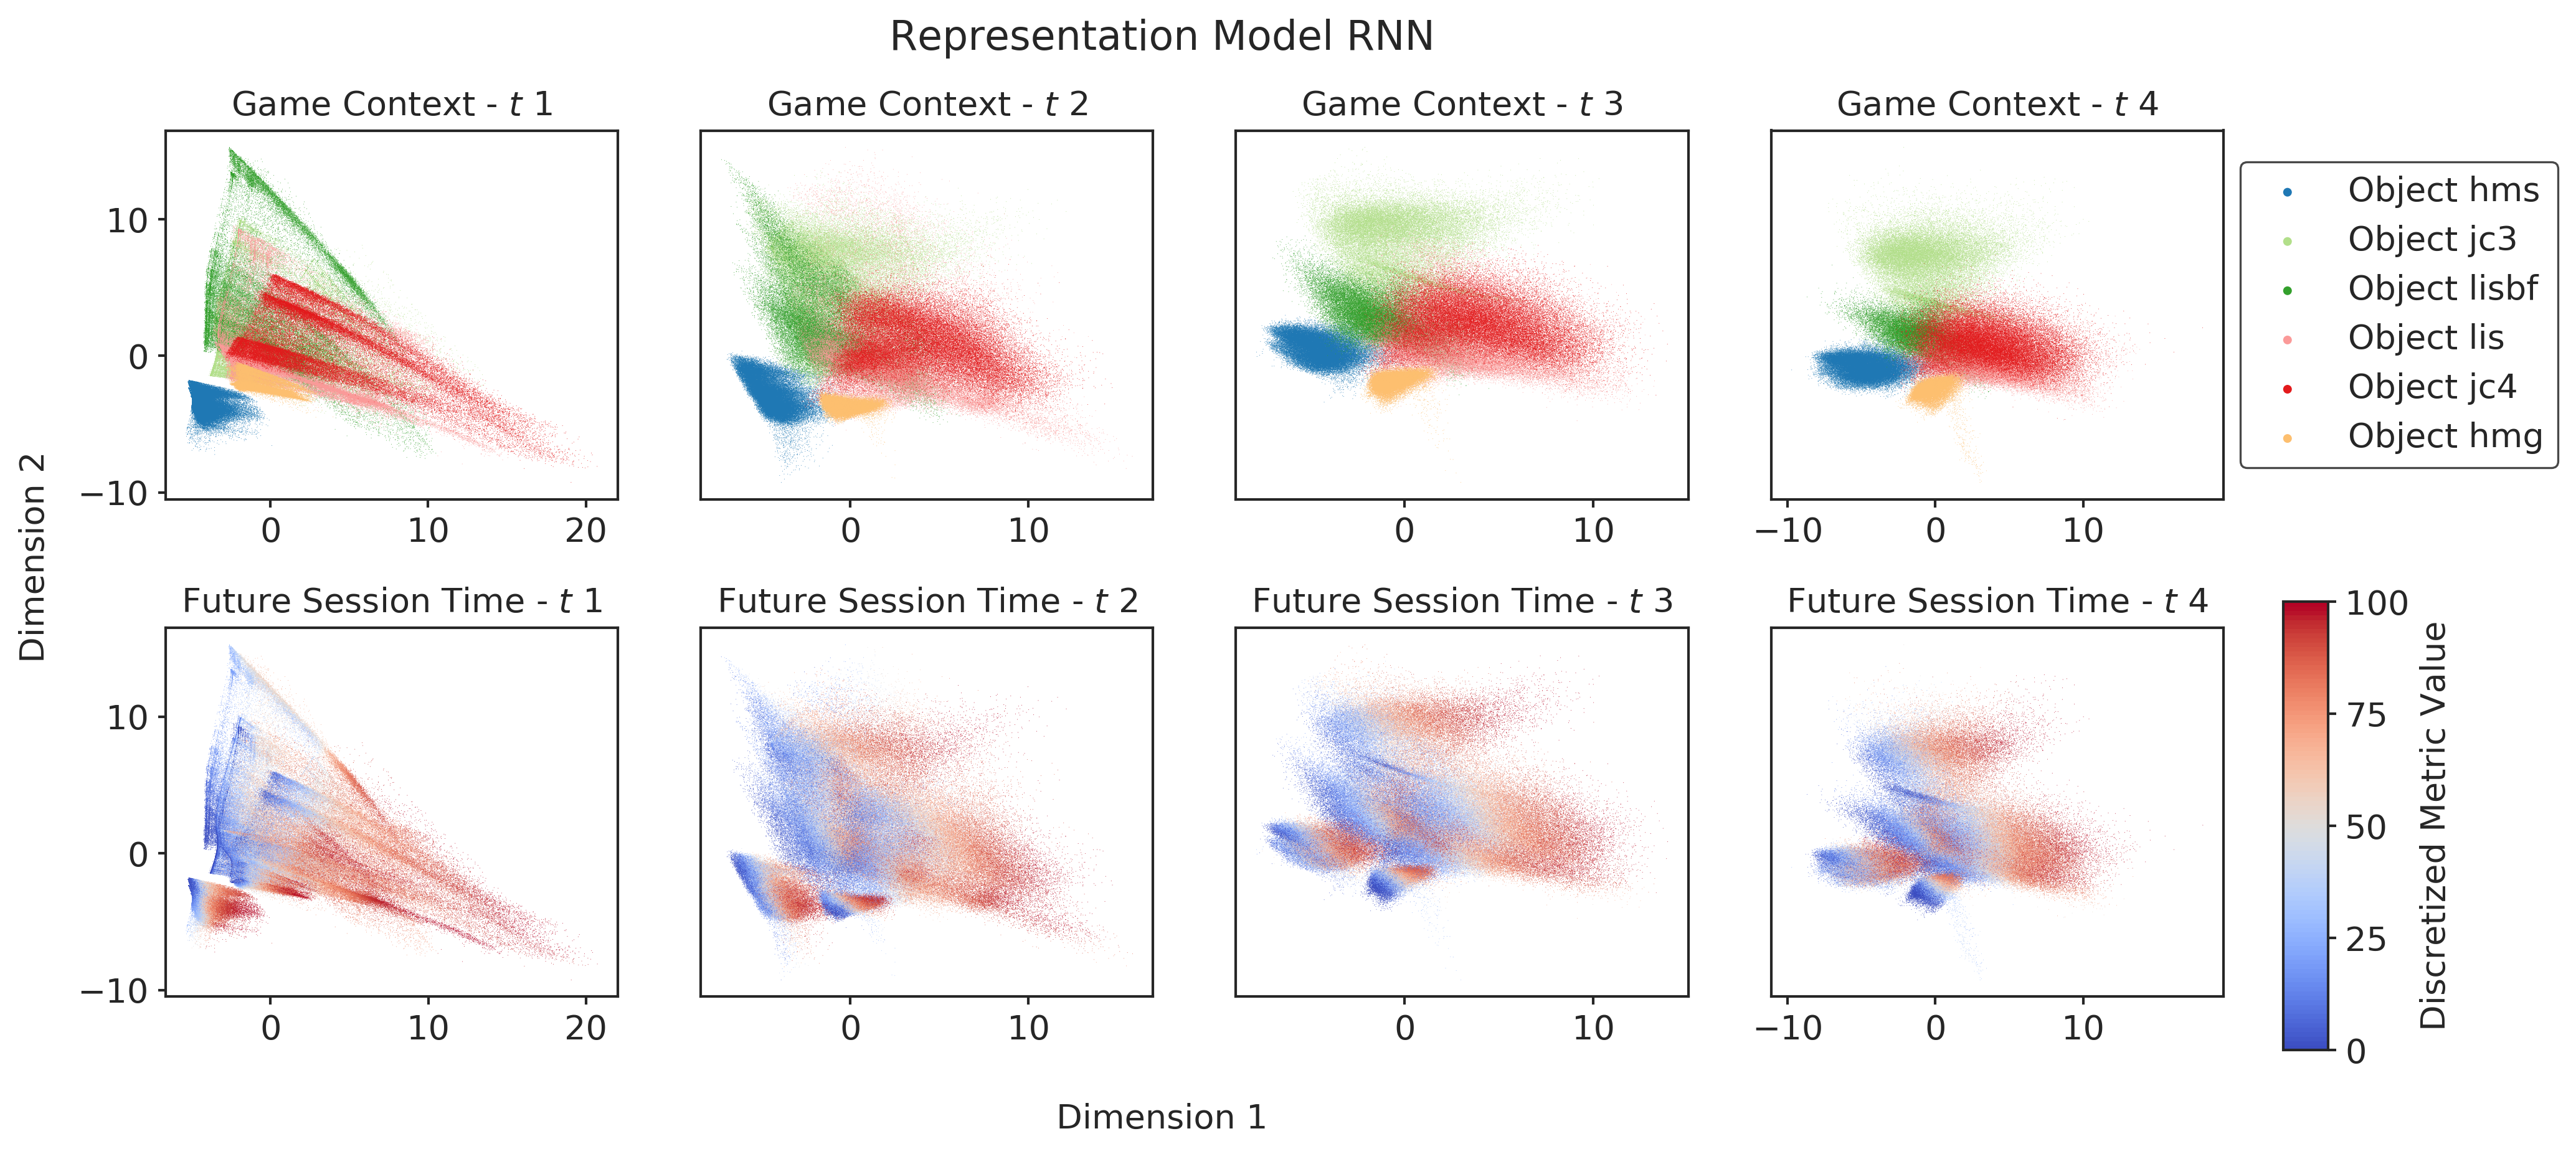
\includegraphics[width=\textwidth]{images/chapter_4/rnn_future_sess_pca.png}
\caption[\textbf{Lower dimensional representation of the latent state generated by the RNN architecture using PCA}]{The figure shows the two-dimensional projection, produced by PCA, of the multi-dimensional representation inferred by the RNN for interactions going from $t1$ to $t4$. We can read the values of the x and y axes as the first two directions of maximum variation in the latent representation. Each point indicates the representation inferred by the RNN model after observing one game session from a single user. The colours in the first row indicate the game object from which the representation is coming. Colours in the second row represent the discounted sum of all future predictions for a particular target (for example, estimated Future Session Time) $\widehat{B}_{t2:T}$ which is given by $\sum_{i=0}^{t2:T} \gamma^i\widehat{B_i}$ with $\gamma=0.1$ as illustrated in the TD Learning equation \ref{td_v}}
\label{temporal_panel_rnn_pca}
\end{figure}

we can see that the representation seems to embed a single gradient line that distinguishes individuals based on the expected length of their future interactions (here future session time) with the considered game objects. However, the low dimensional projection appears to be organized in a disorderly manner, with game contexts blending into each other causing the gradient line to look discontinuous. 

The projection produced by the UMAP algorithm, on the other side, appears to provide a better picture of the inherent structure of the inferred representation. Looking at Figure \ref{full_panel_static}A 

\begin{figure}[!htb]
\centering
\includegraphics[width=\textwidth]{images/chapter_4/static_repr_42.png}
\caption[\textbf{Lower dimensional representation of the latent state generated by the RNN architecture}]{The representation generated by the RNN model distinguishes between different game objects while maintaining an overarching organization able to capture variations in the expected intensity of future interactions that individuals will have with a specific game object. Panel A shows the two-dimensional projection, produced by UMAP, of the multi-dimensional representation inferred by the RNN at $\mathbf{t1}$ as produced by UMAP. We can read the values of the x and y axes as a coordinate system where proximity represents similarity between points in the original high-dimensional space. Each point indicates the representation inferred by the RNN model after observing one game session from a single user. The colours in the Game Context panel indicate the game object from which the representation is coming. Colours in the small panels represent the discounted sum of all future predictions for a particular target (for example, estimated Future Session Time) $\widehat{B}_{t2:T}$ which is given by $\sum_{i=0}^{t2:T} \gamma^i\widehat{B_i}$ with $\gamma=0.1$ as illustrated in equation \ref{td_v}. Each unit  encodes the intensity of future interactions through multiple non-monotonic functions. Panels B and C show the relationship between the activation of randomly-selected hidden units in the LSTM layer of the RNN and the model's predictions at $\mathbf{t1}$. Panel B shows the relationship between the discretized activation of 10 randomly selected units (artificial neurons) plotted along the y axis and the predictions made by the model at $t1$ (colour coded from blue to red as in the small panels in A) for the game object $hmg$. Panel C shows in more detail the relationship between discretized activation and RNN predictions for a single unit highlighted by a black box in Panel B. Here the x axis indicates the discretized activation while the y axis the mean discretized discounted sum of all future predictions produced by the model. Vertical lines are standard errors of the mean. The red curve is the line of best fit provided by a generalized additive model \cite{serven2018} while the box reports the MIC and the correlation coefficient (Spearman's $\rho$) between the artificial neuron activation and the model's predictions.}
\label{full_panel_static}
\end{figure}

we observe how the model was able to effectively distinguish between different game objects while simultaneously encoding for variations in the expected intensity of future interactions. This is illustrated by the fact that each game object occupies different and distinct regions in the representation space while showing a within-object gradient-like organization that places individuals (i.e. single dots) on a continuum based on the estimated magnitude of their future behaviour. 

This organization is preserved for each of the six targets showing how the representation inferred by the model is a suitable meta-descriptor for different behavioural indicators. As expected, some targets show a very similar but not identical organization (e.g. Future Session Time and Future Session Activity) while others appear to be independent (e.g. Future Session Time and Future Absence). We note that the absolute location of each game aggregate (i.e. all the points belonging to a specific game object) on the 2D plane is arbitrary. 

Panels \ref{full_panel_static}B and \ref{full_panel_static}C provide more insight into the activation profiles of individual hidden units constituting the generated representation. Panel \ref{full_panel_static}B shows the relationship between the activity of 10 randomly-chosen units and the predictions generated for the five targets. These are essentially transducer functions illustrating how the estimate for a particular target varies (on average) as the output of a units increases or decreases. Each unit seems to encode for multiple non-monotonic functions, one for each of the considered targets. Differences in the shape of these functions reflect similarities between their associated targets. For example, the functions associated to two highly related targets like Future Session Time and Future Session Activity (see panel \ref{full_panel_static}A) appear to be very similar in shape (see panels \ref{full_panel_static}B and \ref{full_panel_static}C). Interestingly, although most units appear to encode for unique functions some of them (e.g. 41 and 44) show an almost identical behaviour. This suggests the presence of redundancy in the functions underlying the representation generated by the RNN model. These observations are clarified in panel \ref{full_panel_static}C, where the functions associated with a single unit (20, indicated by a dark box in \ref{full_panel_static}B) are presented. Here we observe a strong, non-linear relationship between the unit's activity and the estimated targets (see the high MIC values and the line of best fit). In addition, the between-targets variation in MIC values suggest how the chosen unit is not equally informative for all targets but rather shows specialized  behaviour.

\begin{figure}[!htb]
\centering
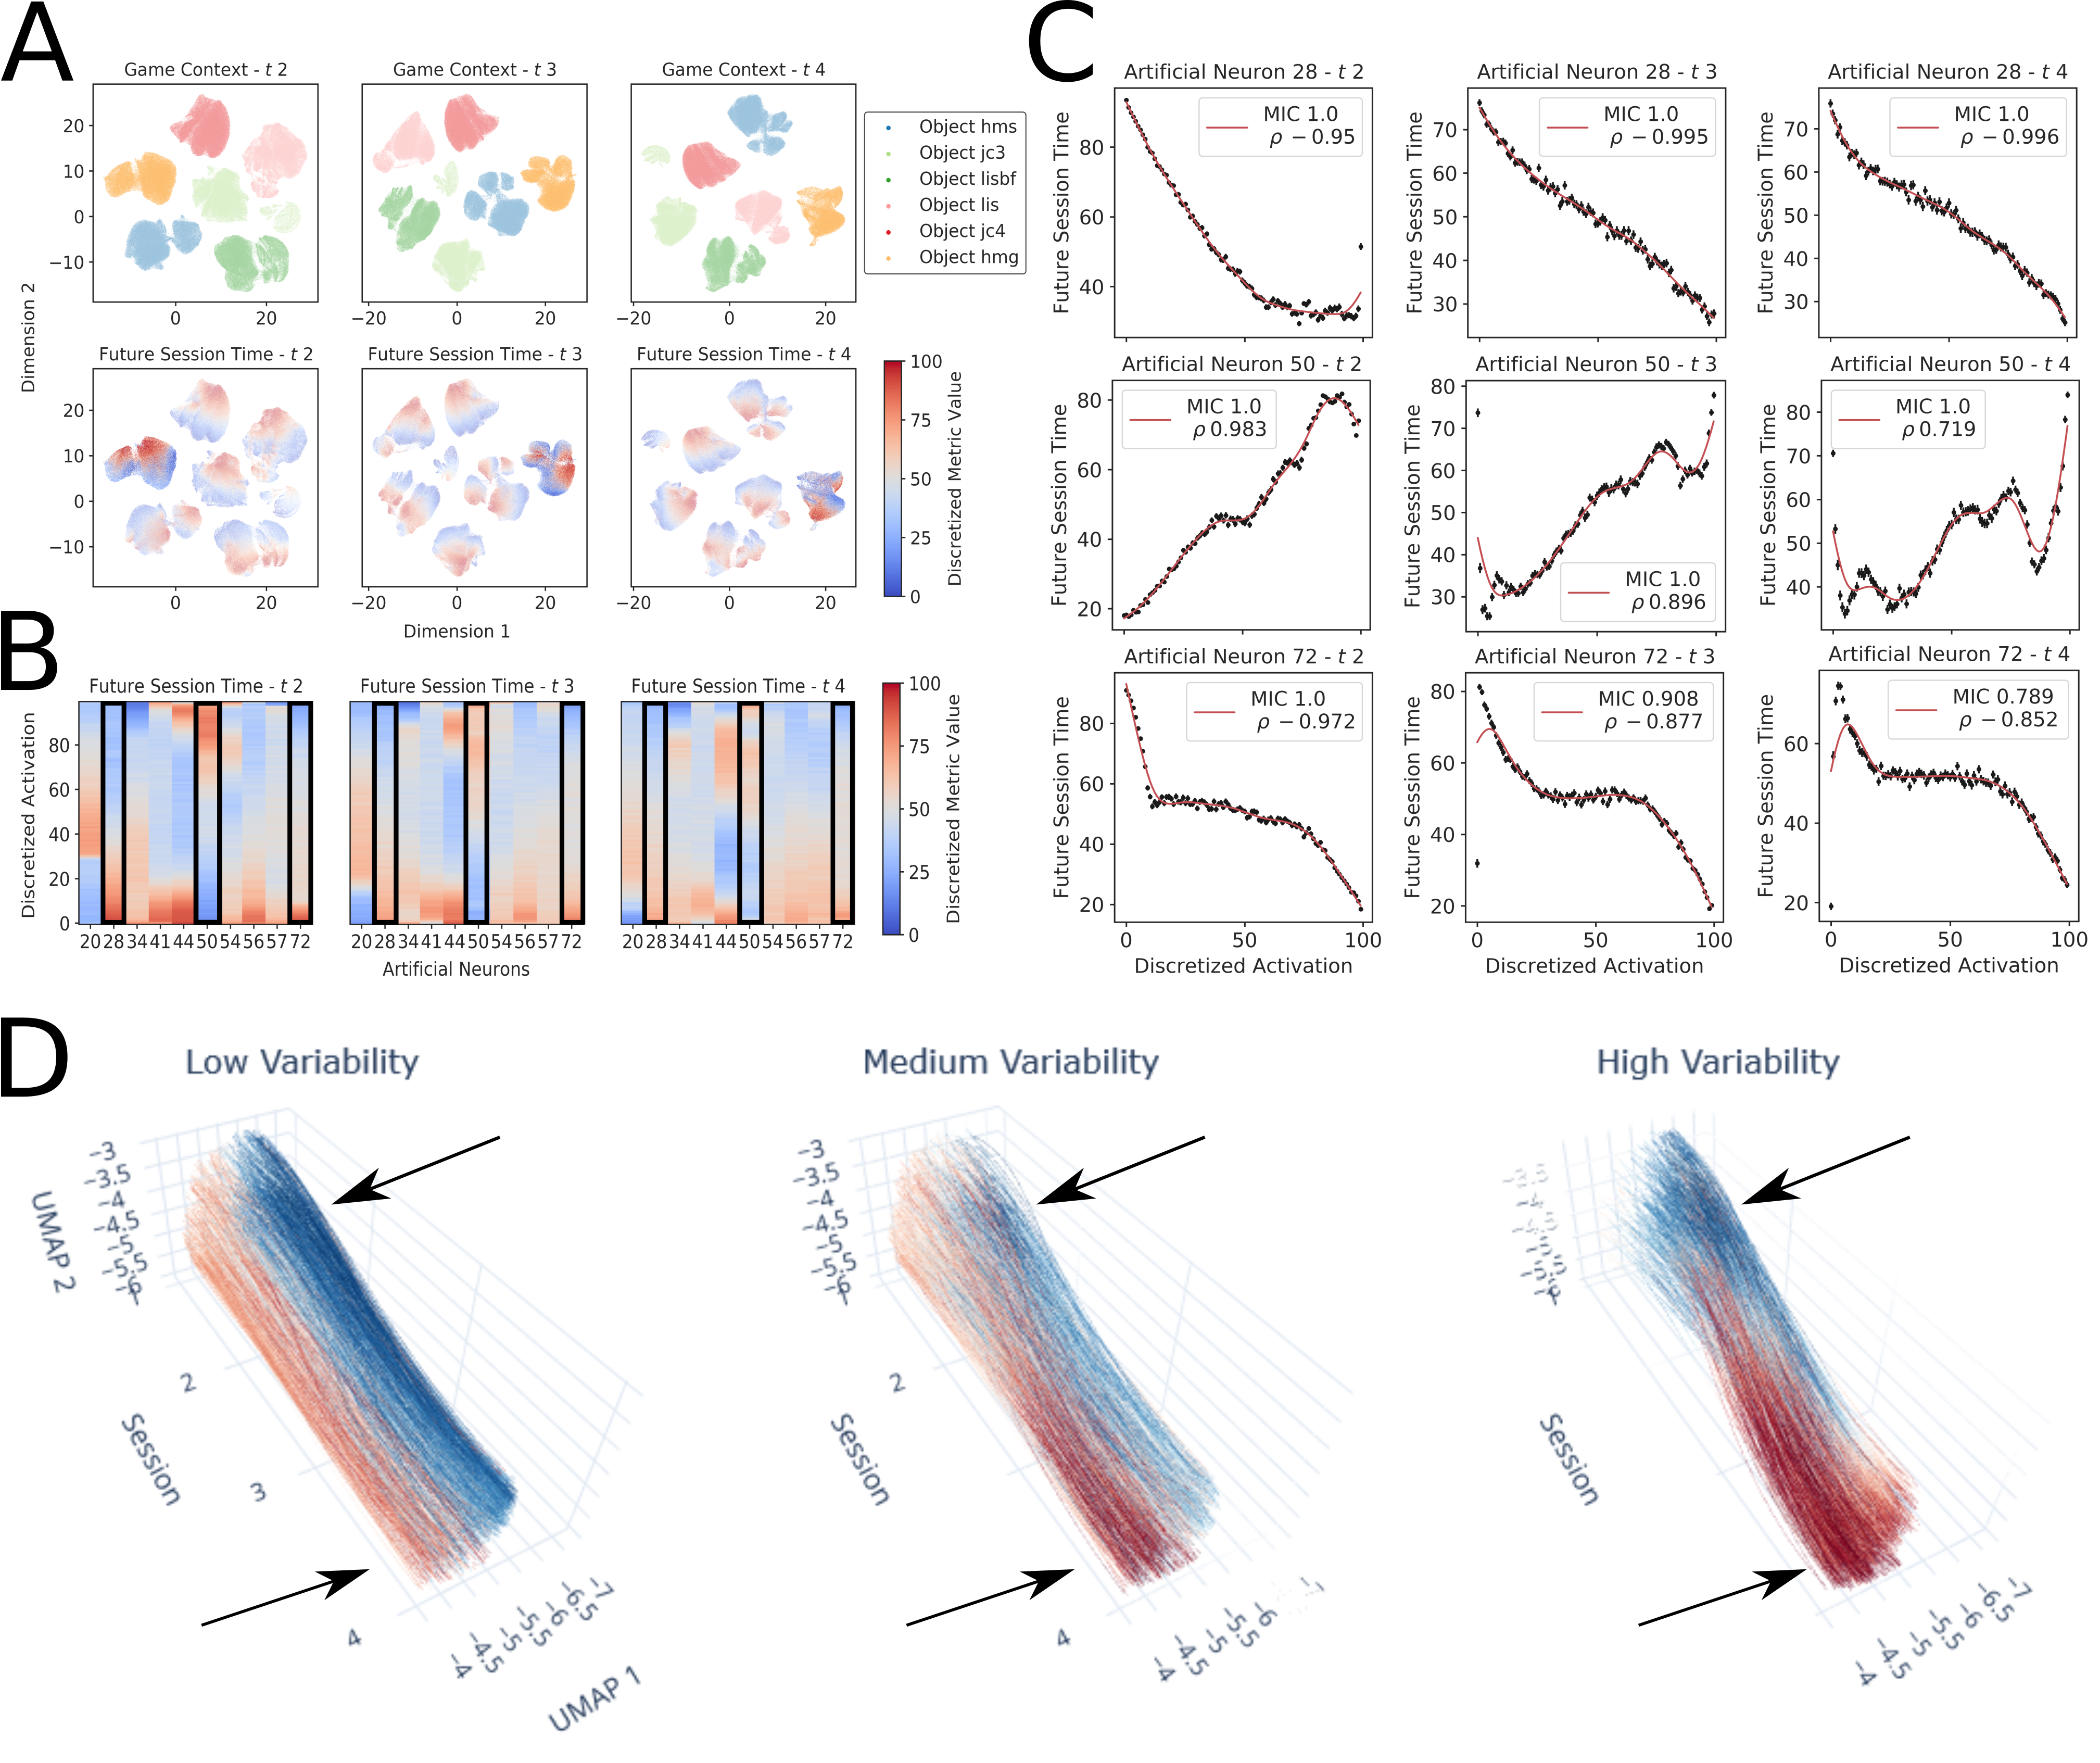
\includegraphics[width=\textwidth]{images/chapter_4/dynamic_repr_42.png}
\caption[\textbf{Lower dimensional representation of the evolution of the latent states generated by the RNN architecture}]{The representation generated by the RNN model appears to maintain its discriminant properties over time. Panel A shows a two-dimensional projection of the multi-dimensional representation inferred by the RNN at $t2$, $t3$ and $t4$. The inferred representation maintains its gradient-like organization over time with an increased ability to differentiate between game objects. As in Figure \ref{full_panel_static}, x and y axes are dimensions individuated by the UMAP algorithm and can be interpreted as a coordinate system where proximity represents similarity between points. Colours in the first row indicate which game object the representation is coming from while those in the second row indicate the discounted sum of future predictions for a single target (i.e. "Future Session Time"). \textbf{The units constituting the generated representation encode for functions that are consistent over time.} Panels B and C show the relationship between units' activation and the model's predictions over time for the game object $hmg$. Different units appear to encode the same target with different non non-monotonic functions which are relatively consistent over time. Panel B illustrates the relationship between the same 10 randomly selected units specified in figure \ref{full_panel_static} and the predictions made by the model for Future Session Time at $t2$, $t3$ and $t4$. Panel C shows in more detail the relationship of the three artificial neurons, highlighted by black boxes in B, across time. Each row is a different unit while each column corresponds to a different $t$. The x axis indicates the discretized activation while the y axis the mean discretized discounted sum of all future predictions. Vertical lines are standard errors of the mean. The red curve is the line of best fit provided by a generalized additive model \cite{serven2018} while the box report the MIC and the correlation coefficient (Spearman's $\rho$) between the artificial neuron activation and the model's predictions. \textbf{The generated representation produces areas of low and high expected intensity among which individuals move over time.} Panel D shows trajectories through time produced by a version of UMAP that incorporates temporal information. Data are drawn from random subsets of individuals having low, medium and high variability in their expected amount of future behaviour. The representation inferred by the RNN model produces "hot" (i.e. the left side) and "cold" (i.e. the right side) regions, representing high and low expected Future Session Time, that are spatially consistent over time. Individuals appear to either stay in the same region or to move between regions over time. Here each line represents variations in the representation generated by the RNN model for a single user over four temporal steps. Continuity is generated by means of cubic spline interpolation for the lines and by linear interpolation for the colours. The x and y axes are the dimensions individuated by the UMAP algorithm while the z axis indicates the associated point in time. Colours indicate the discounted sum of future predictions produced by the model at a specific point in time.}
\label{full_panel_temporal}
\end{figure}

The analyses in Figure \ref{full_panel_static} were performed at a single time point $t1$. However, as we mentioned before, the characteristics of our architectures allowed us to also evaluate how the latent representation evolved over time. 

Looking at Figure \ref{full_panel_temporal}, we can see that the characteristics detected at a single point in time remain qualitatively consistent over time. For example, focusing on Future Session Time (see Appendix \ref{rnn_architecture_representations} for results connected to other targets), we see in Figure \ref{full_panel_temporal}A that the model's ability to segregate different game objects while providing an  overarching representation of the intensity of future interactions is preserved over time. This supports the hypothesis that the representation inferred by our model is dynamic in nature which is further corroborated by panel \ref{full_panel_temporal}D. There we can see how the RNN model was able to individuate a "space" with temporally consistent ”hot” and ”cold” regions between which individuals gradually moved over time depending on the expected intensity of their future interactions. This means that given the history of interaction of a particular individual with a specific game object, our model would determine their "position" (i.e. their "internal state") in a latent space indicative of the expected intensity of future interactions with that object. If we recall our definition of attributed incentive salience from chapters \ref{chapter_lit_review} and \ref{chapter_theory_modelling} we can suggest that the model has inferred the location of individuals in what is an approximation (from the functional point of view) of the "attributed incentive salience space". This aligns with the manifold hypothesis mentioned in sections \ref{manifold_rep_incentive_salience} and \ref{manifold_learning}: changes in the propensity to interact with a specific game object (i.e. variations in the amount of attributed incentive salience) can be expressed moving on a manifold embedded within an $h$ dimensional space, with $h$ being the dimensionality of the representation generated by our RNN model. 

It appears that the hidden units constituting this representation tend to be consistent over time in the type of functions they encode (see Figure \ref{full_panel_temporal}B and C). As expected, we can again observe a strong non linear association between units' activation and targets' predictions, see MIC values and lines of best fit. The decrease in MIC value observed in Figure \ref{full_panel_temporal}C for the artificial neuron 72 might indicate how certain units lose their informative power over time.

\begin{figure}[!htb]
\centering
\includegraphics[width=\textwidth]{images/chapter_4/RNN_MLP_repr_42.png}
\caption[\textbf{Lower dimensional representation of the latent states generated by the time-distributed MLP architecture}]{The representation generated by the MLP model is less effective at distinguishing between different game objects and different levels of expected future behaviour intensity. Panel A shows a two-dimensional projection of the multi-dimensional representation inferred by the MLP at $t1$, $t2$, $t3$ and $t4$. Differently from the RNN, the representation shows a disruption in the gradient-like organization and a reduced ability to differentiate between game objects which remain constant over time. The x and y axes are dimensions individuated by the UMAP algorithm and can be interpreted as a coordinate system where proximity represents similarity between points. Colours in the first row indicate which game object the representation is coming from while those in the second row indicate the discounted sum of future predictions for a single target (i.e. "Future N° of Sessions") \textbf{The representation generated by the MLP model is less effective at at distinguishing different levels of expected behaviour intensity for states that are further away in the future.} Panel B shows a two-dimensional projection of the multi-dimensional representation inferred by the RNN (left) and MLP(right) at $t1$ but colour coded with the discounted sum of future predictions from $t4$ onward. The representation generated by the RNN is able to maintain a gradient-like organization even from states that are further away in the future while this capacity is almost entirely lost for the MLP. The colours in the Game Context panel indicate the game object from which the representation is coming. Colours in the small panels represent the discounted sum of all future predictions for a particular target computed from $t4$ onward instead that from $t1$. The x and y axes are the dimensions individuated by the UMAP algorithm.}
\label{predictive_panel}
\end{figure}

If we look at the differences between MLP and RNN-like architectures from section \ref{model_architecture_2}, we can see that they all aim to solve the same task: predict the intensity of future behaviour given the history of interactions. They do so relying on the same type of metrics, leveraging similar computational mechanisms (i.e. multitask learning and non-linearity) and producing representation according to the same underlying principle (i.e. the manifold hypothesis). Nevertheless, the fact that MLP architectures consistently provided poorer fit to data already suggests that whatever representation it had inferred it was likely a sub-optimal approximation of the manifold structure of attributed incentive salience. 

Looking at figure \ref{predictive_panel}A, and knowing that UMAP represents differences and similarities between points through distance, we can see how the representation generated by the MLP less clearly differentiate between game objects. On the same figure, we can notice how the gradient representation for the metric Future N° Sessions is largely disrupted. This effect is however consistently less pronounced for other metrics (see Appendix \ref{mlp_architecture_representations} for additional visualizations) and in accordance to the differences in predictive perfromance that we observed in chapter \ref{chapter_implementation_testing}. 

Recalling what mentioned in section \ref{comp_framework}, the latent state produced by the level of attributed incentive salience should retain at any point in time some predictive power over the intensity of all the future interactions (i.e. not just the one that follows). Figure \ref{predictive_panel}B shows the representation generated by RNN and MLP at $t1$ but color coded with the discounted sum of the predictions made from $t4$ onward. We can see that, even if degraded, RNN still preserves some of the desired gradient-like organization which is instead much more disrupted for MLP. This is in accordance to what is shown by Figure \ref{full_panel_temporal}D: the RNN appears to define regions of high and low expected behavioural intensity which are consistent over time rather than generating representations that are mostly representative of what is expected at $t+1$.

\subsection{Evaluating the Contribution of Environmental and Game Events Covariates}
\label{representation_env_even_contr}
Shifting our attention to the representations generated by the improved version of the RNN architecture we can see some noticeable differences. Looking at Figure \ref{rnn_env_even_full_beha} 

\begin{figure}[!htb]
\centering
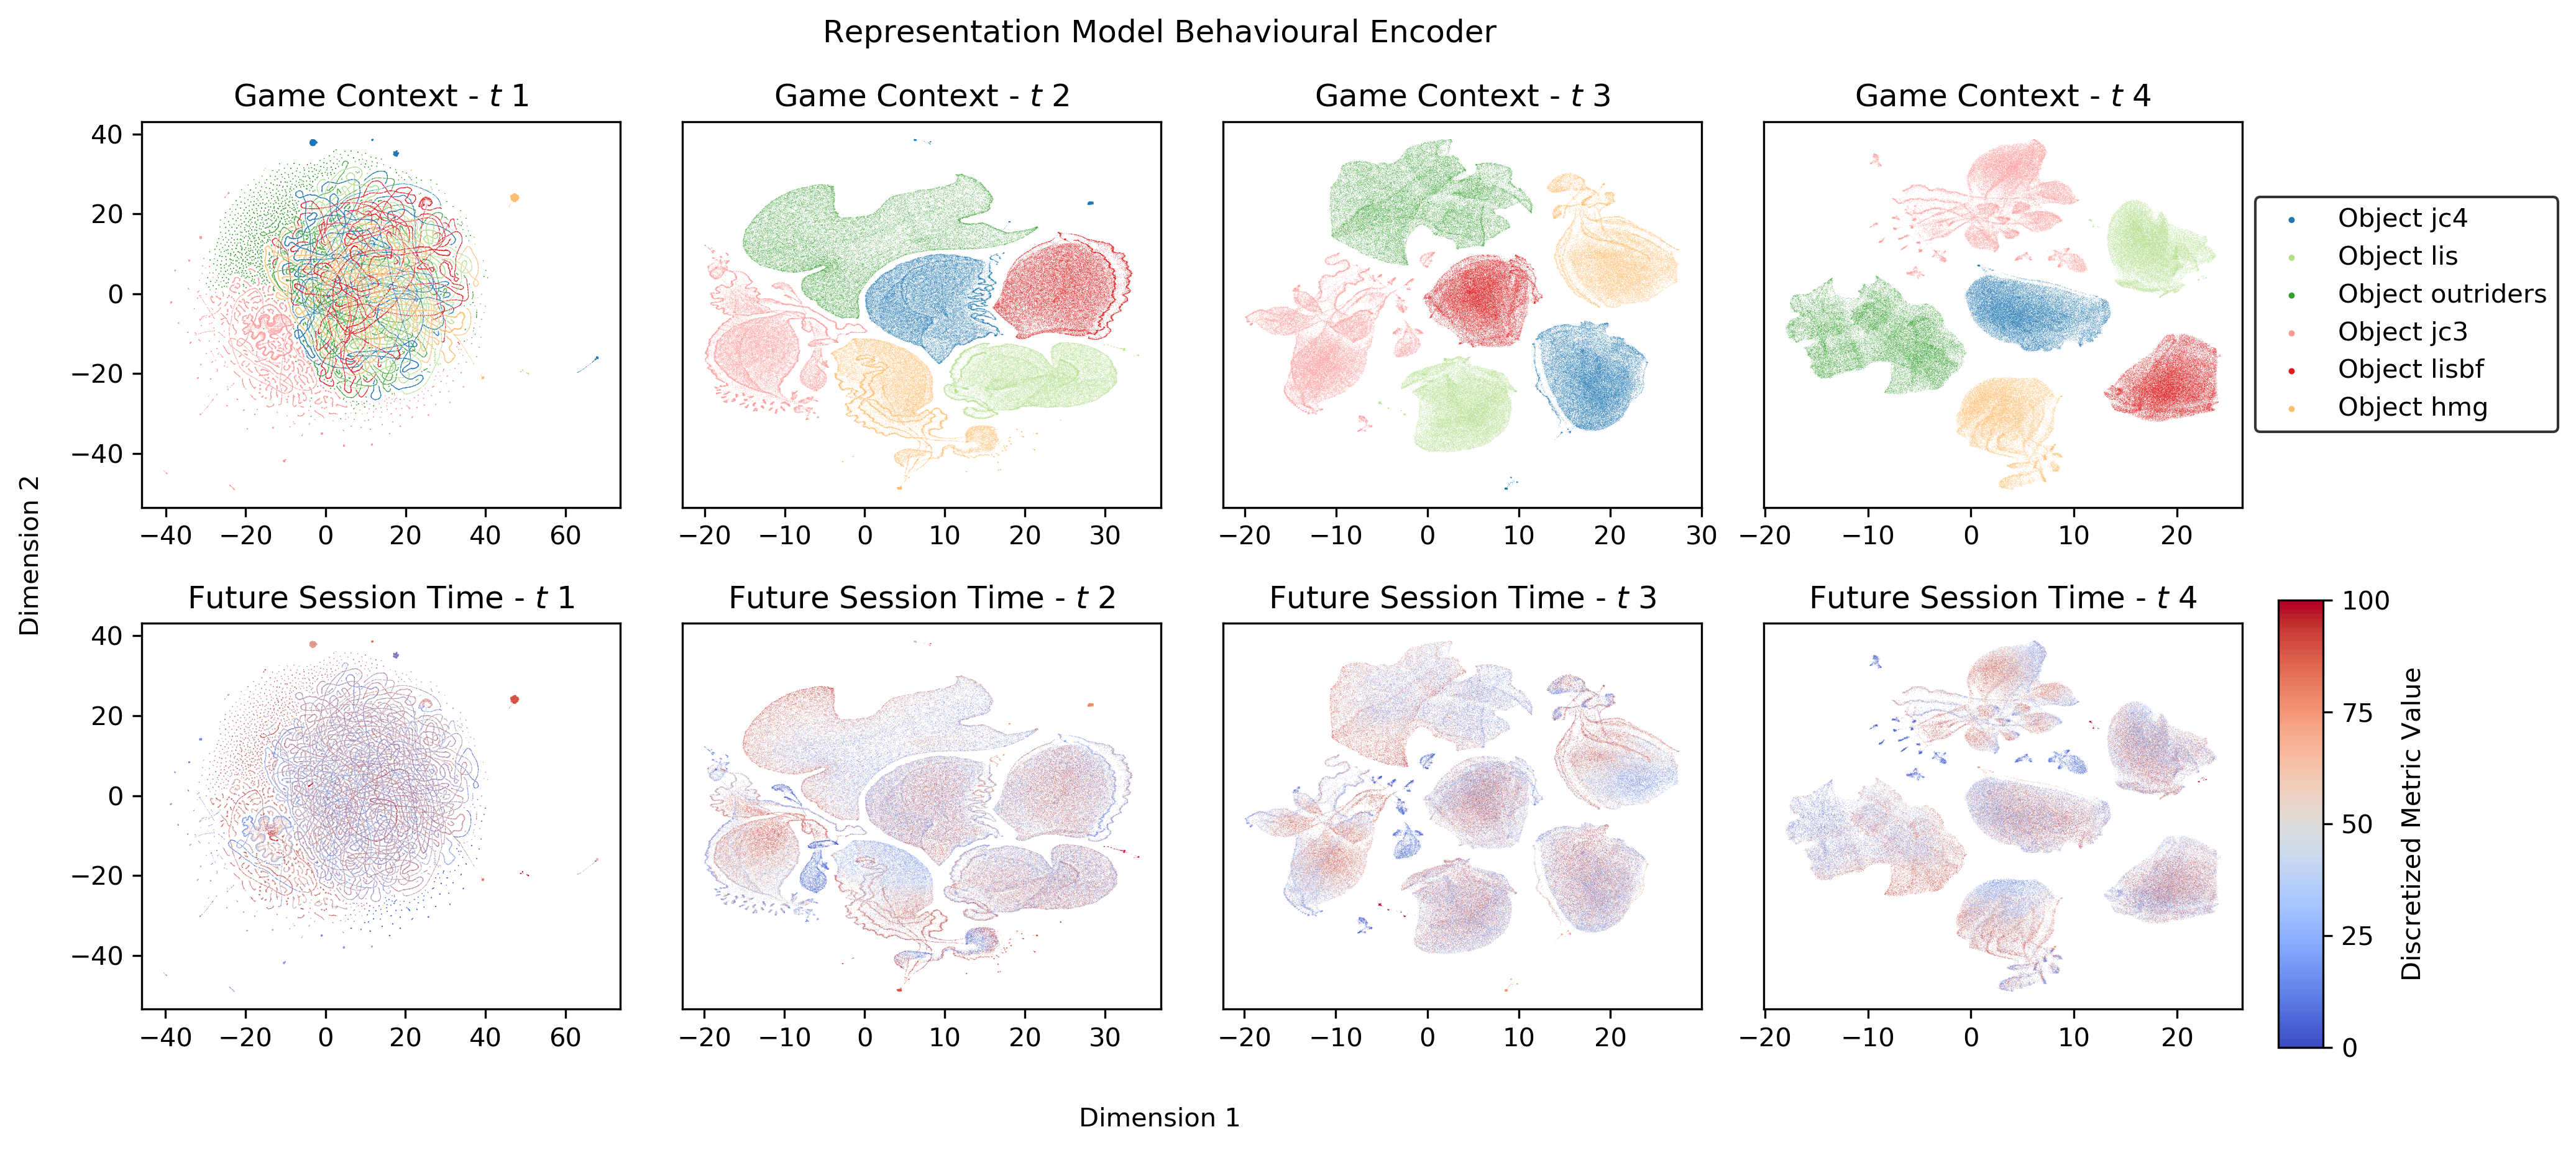
\includegraphics[width=\textwidth]{images/chapter_4/RNN_env_even_0_lstm_layer_features_Future Session Time.png}
\caption[\textbf{Lower dimensional representation of the latent representations generated by the improved version of the RNN architecture from the behavioural metrics}]{Each panel shows a two-dimensional projection of the multi-dimensional representation inferred by the improved RNN architecture at $t1$, $t2$, $t3$ and $t4$. The representations presented in this figure have been generated by the portion of the architecture receiving the behavioural metrics as input. As in Figure \ref{full_panel_temporal}, x and y axes are dimensions individuated by the UMAP algorithm and can be interpreted as a coordinate system where proximity represents similarity between points. Colours in the first row indicate which game object the representation is coming from while those in the second row indicate the discounted sum of future predictions for a single target (i.e. "Future Session Time").}
\label{rnn_env_even_full_beha}
\end{figure}

we can see how the representation generated from the behavioural metrics changes considerably from the simple RNN architecture. Despite the ability to differentiate between game objects is, up to a certain degree, preserved, the quality of the gradient organization is markedly diminished. This is doesn't come as a surprising result: similarly to what happens when covariates are added in a linear model, the behavioural metrics are now only one of the components making up the final representation in charge of producing the model's predictions. It is however worth noticing that the ability to differentiate between individuals with respect to the intensity of their future interactions is not completely removed suggesting the intensity of past interactions still plays a role in determining the intensity of future ones. 

The same cannot be said for the representation generated by the environmental metrics. If we look at Figure \ref{rnn_env_even_full_env} we can see that not just the ability to differentiate between game objects is almost completely disrupted, but also the capacity to distinguish between individuals with high and low expected intensity of future interactions. 

\begin{figure}[!htb]
\centering
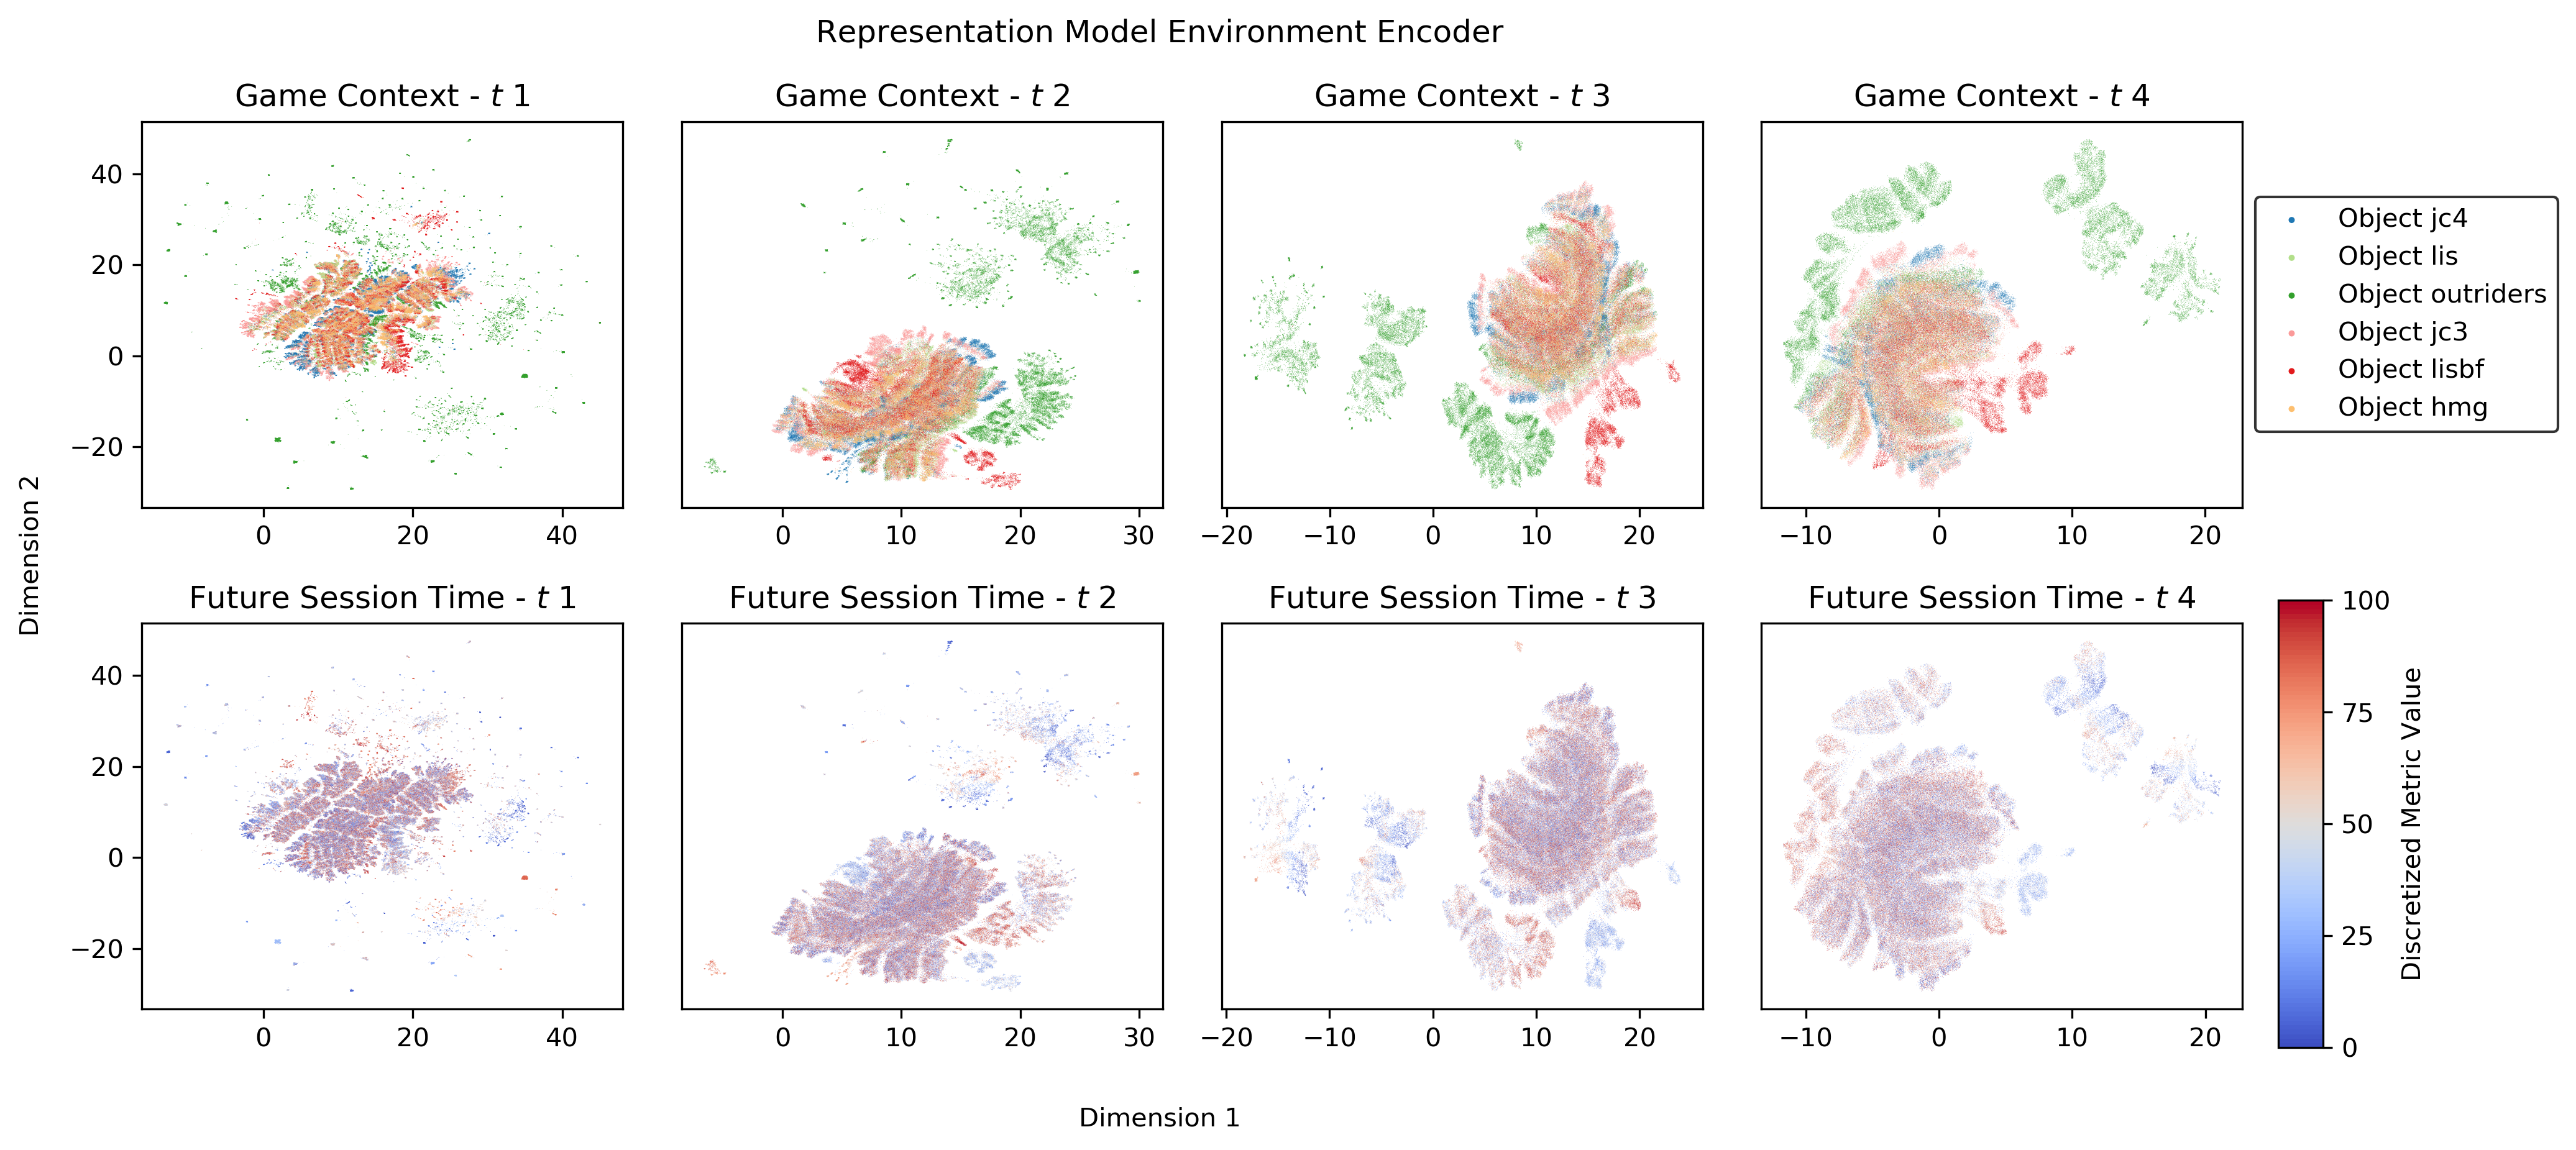
\includegraphics[width=\textwidth]{images/chapter_4/RNN_env_even_0_lstm_layer_env_Future Session Time.png}
\caption[\textbf{Lower dimensional representation of the latent representations generated by the improved version of the RNN architecture from the environmental metrics}]{Each panel show a two-dimensional projection of the multi-dimensional representation inferred by the improved RNN architecture at $t1$, $t2$, $t3$ and $t4$. The representation presented in this figure has been generated by the portion of the architecture receiving the environmental metrics as input. As in Figure \ref{full_panel_temporal}, x and y axes are dimensions individuated by the UMAP algorithm and can be interpreted as a coordinate system where proximity represents similarity between points. Colours in the first row indicate which game object the representation is coming from while those in the second row indicate the discounted sum of future predictions for a single target (i.e. "Future Session Time").}
\label{rnn_env_even_full_env}
\end{figure}

As we anticipated in sections \ref{model_architecture_3} and \ref{modelling_env_and_game_elements}, we did not expect the environmental variables to have strong predictive power on future ammount of gaming behaviour, but rather to act as an absorbing factor for possible noise observed in the behavioural metrics. Or better, we argued that environmental factors might affect the behavioural manifestations of a certain latent state (i.e. attributed incentive salience) both in the past and in the future, but do not play a central role in the shaping of the state itself (i.e. the level of attributed incentive salience). We will expand more on this section \ref{partition_environment}).

Another possibility is that the environmental information do not play a relevant role in generating a latent representation with good predictive power and are just treated as noise by the model. However, by looking at the occasional improvements in predictive performance that they provided in section \ref{results_3}, it seems more plausible that they are to be considered as nuisance metrics supporting the role of the other model inputs. 

The representation generated from the game events information sits in stark contrast to the previous two. Looking at Figure \ref{rnn_env_even_full_events} we can see how different it is from what we observed in Figure \ref{rnn_env_even_full_beha}. The representation appears highly fragmented but with each fragment consistently belonging to distinct game contexts. This suggests the representation attempted to encode the heterogeneity in sequences of game events while maintaining them within the same context.

\begin{figure}[!htb]
\centering
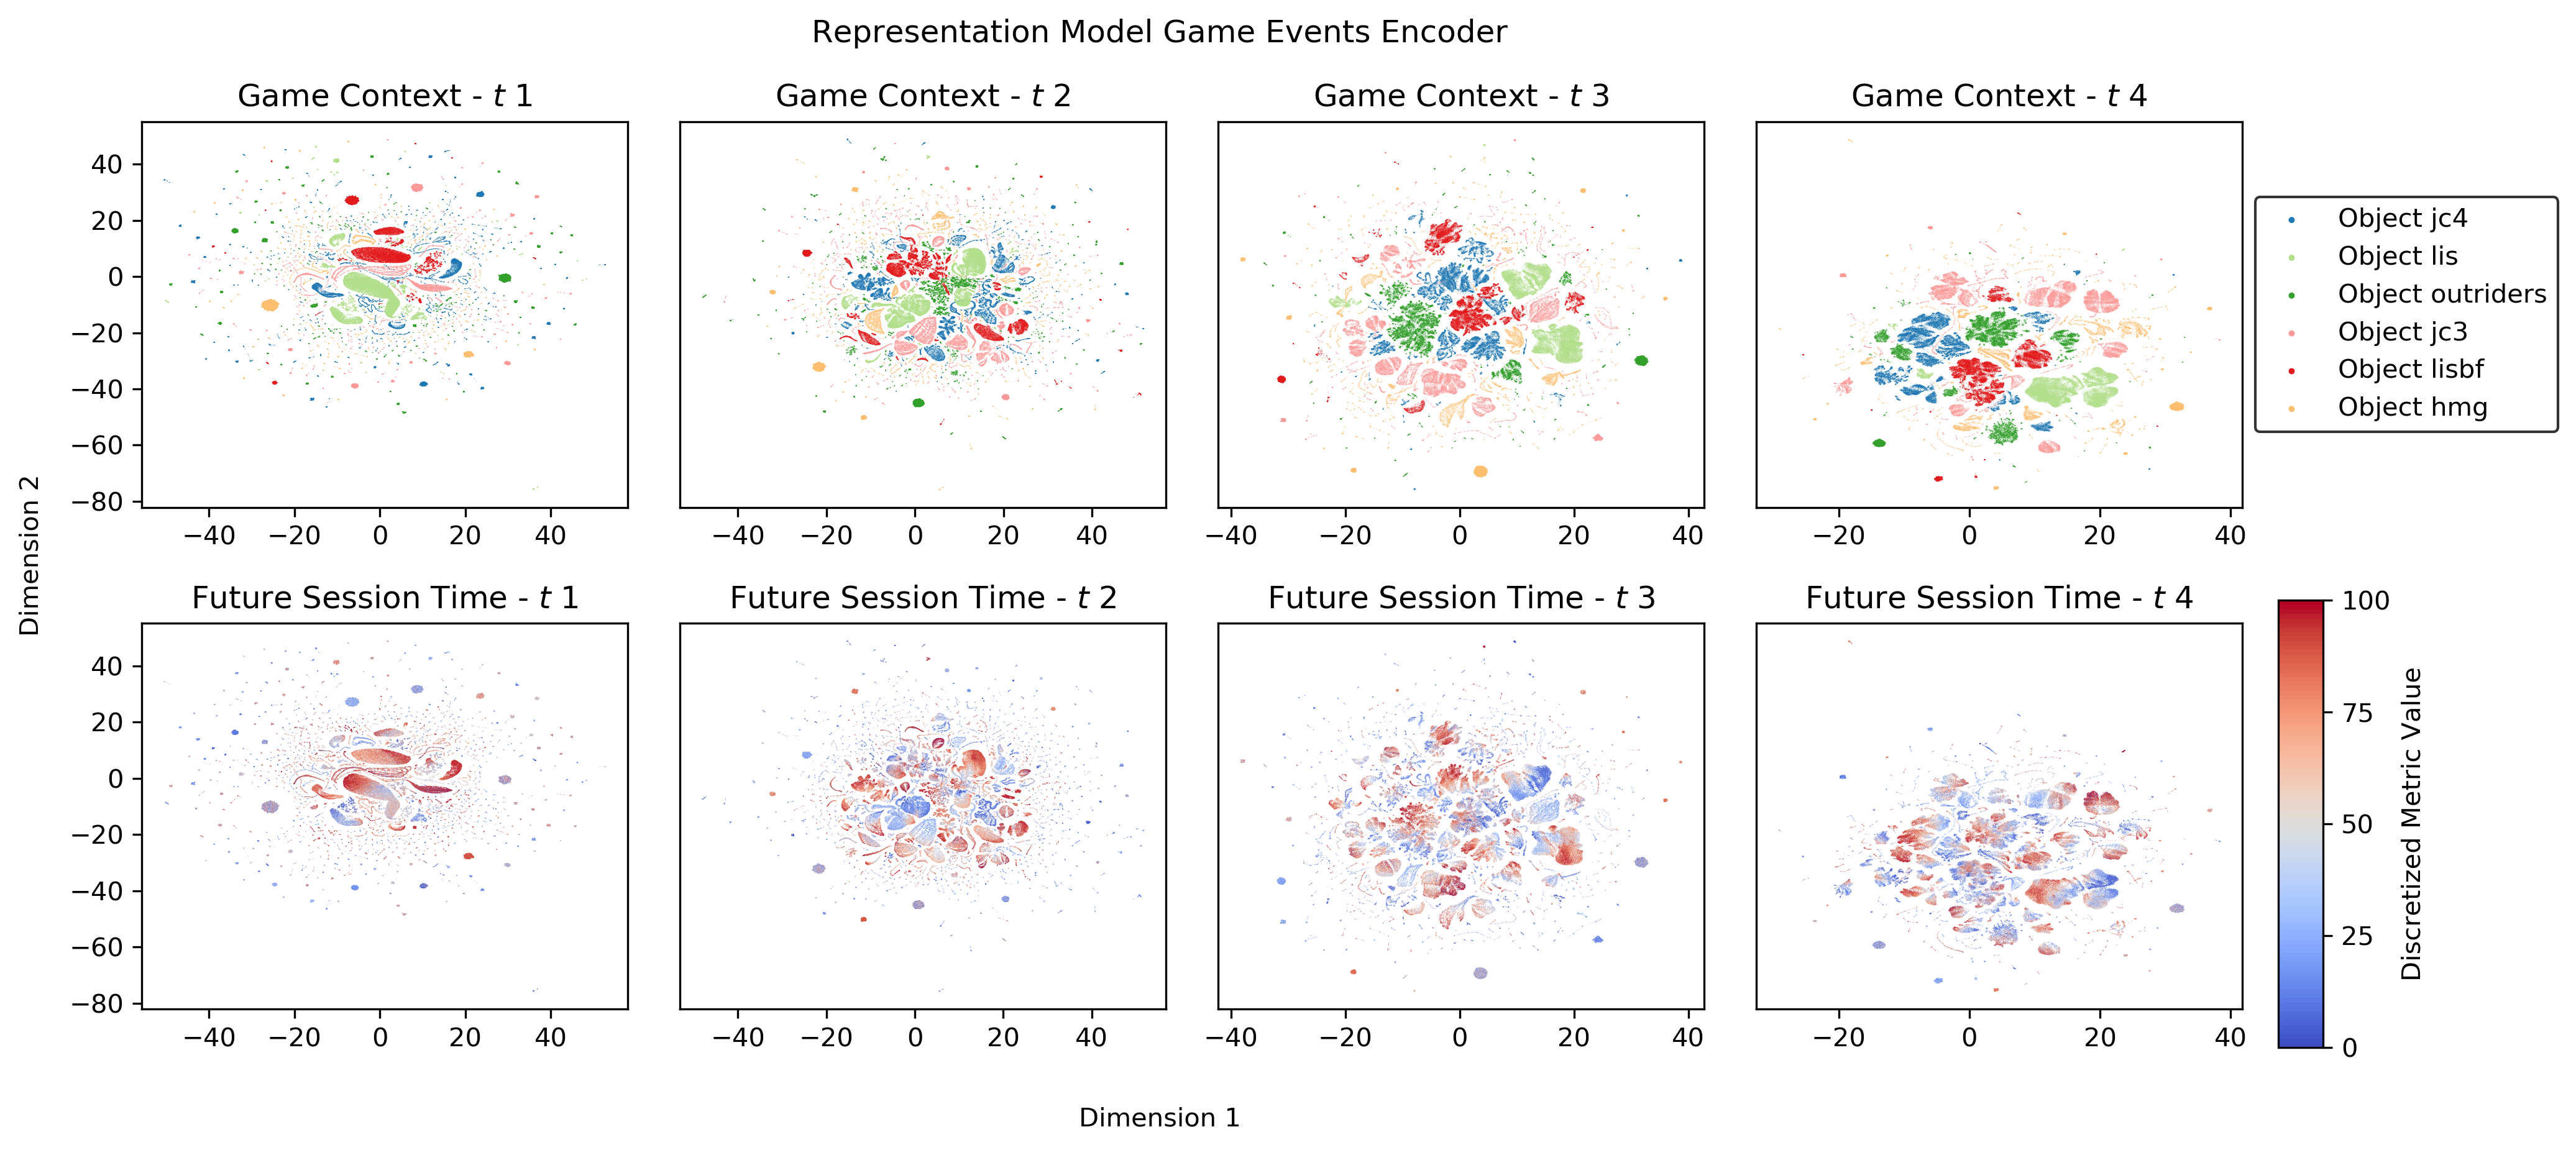
\includegraphics[width=\textwidth]{images/chapter_4/RNN_env_even_0_lstm_layer_events_Future Session Time.png}
\caption[\textbf{Lower dimensional representation of the latent representations generated by the improved version of the RNN architecture from the game events metrics}]{Each panel show a two-dimensional projection of the multi-dimensional representation inferred by the improved RNN architecture at $t1$, $t2$, $t3$ and $t4$. The representation in this figure has been generated by the portion of the architecture receiving the game events metrics as input. As in Figure \ref{full_panel_temporal}, x and y axes are dimensions individuated by the UMAP algorithm and can be interpreted as a coordinate system where proximity represents similarity between points. Colours in the first row indicate which game object the representation is coming from while those in the second row indicate the discounted sum of future predictions for a single target (i.e. "Future Session Time").}
\label{rnn_env_even_full_events}
\end{figure}

The observed level of fragmentation is in line with all the possible sets arising by the combination of the considered game events and their relative frequency of interactions. For example considering the tuple $\{event, frequency\}$ we could have:

\begin{gather}
\label{seq_differences}
    \{\{combat, 10\}, \{explore, 3\}, \{achievement, 2\}\} \\ \nonumber
    \neq \\ \nonumber
    \{\{combat, 2\}, \{explore, 10\}, \{achievement, 5\}\} \\ \nonumber
    \neq \\ \nonumber
    \{\{dialogue, 2\}, \{puzzle, 10\}, \{achievement, 5\}\} \\ \nonumber 
    \neq \\ \nonumber
    \dots
\end{gather}

This type of behaviour is comparable to what can be observed when analyzing the word embeddings of different text corpora (e.g. see the Open Syllabus project \cite{opensyllabus}) and suggest that the architecture was able to discern differences in the sequential choices made by the individuals when interacting with different in-game elements.

What is most interesting however is that among the representations inspected so far, the one generated from the game events metric is the one that best preserves the gradient organization observed for the simple RNN architecture. This suggests that the sequences of observed interactions with specific in-game mechanics plays a role in differentiating between individuals with respect to the expected intensity of their future interactions with a specific game object. This, in turn, is something that we anticipated in sections \ref{factors_engagement} and \ref{modelling_env_and_game_elements} and that is in line with previous findings in the videogame literature \cite{makarovych2018like}.

Finally, when looking at the shared representation in Figure \ref{rnn_env_even_full_shared}, we can see how it resembles the one generated by the simplified version of the RNN architecture with the only difference being a more clearly defined gradient organization. This representation is functionally equivalent to the one extracted by the simplified RNN architecture (i.e. it is used for performing multi-task learning) and is hypothesized to approximate the manifold structure of attributed incentive salience.

\begin{figure}[!htb]
\centering
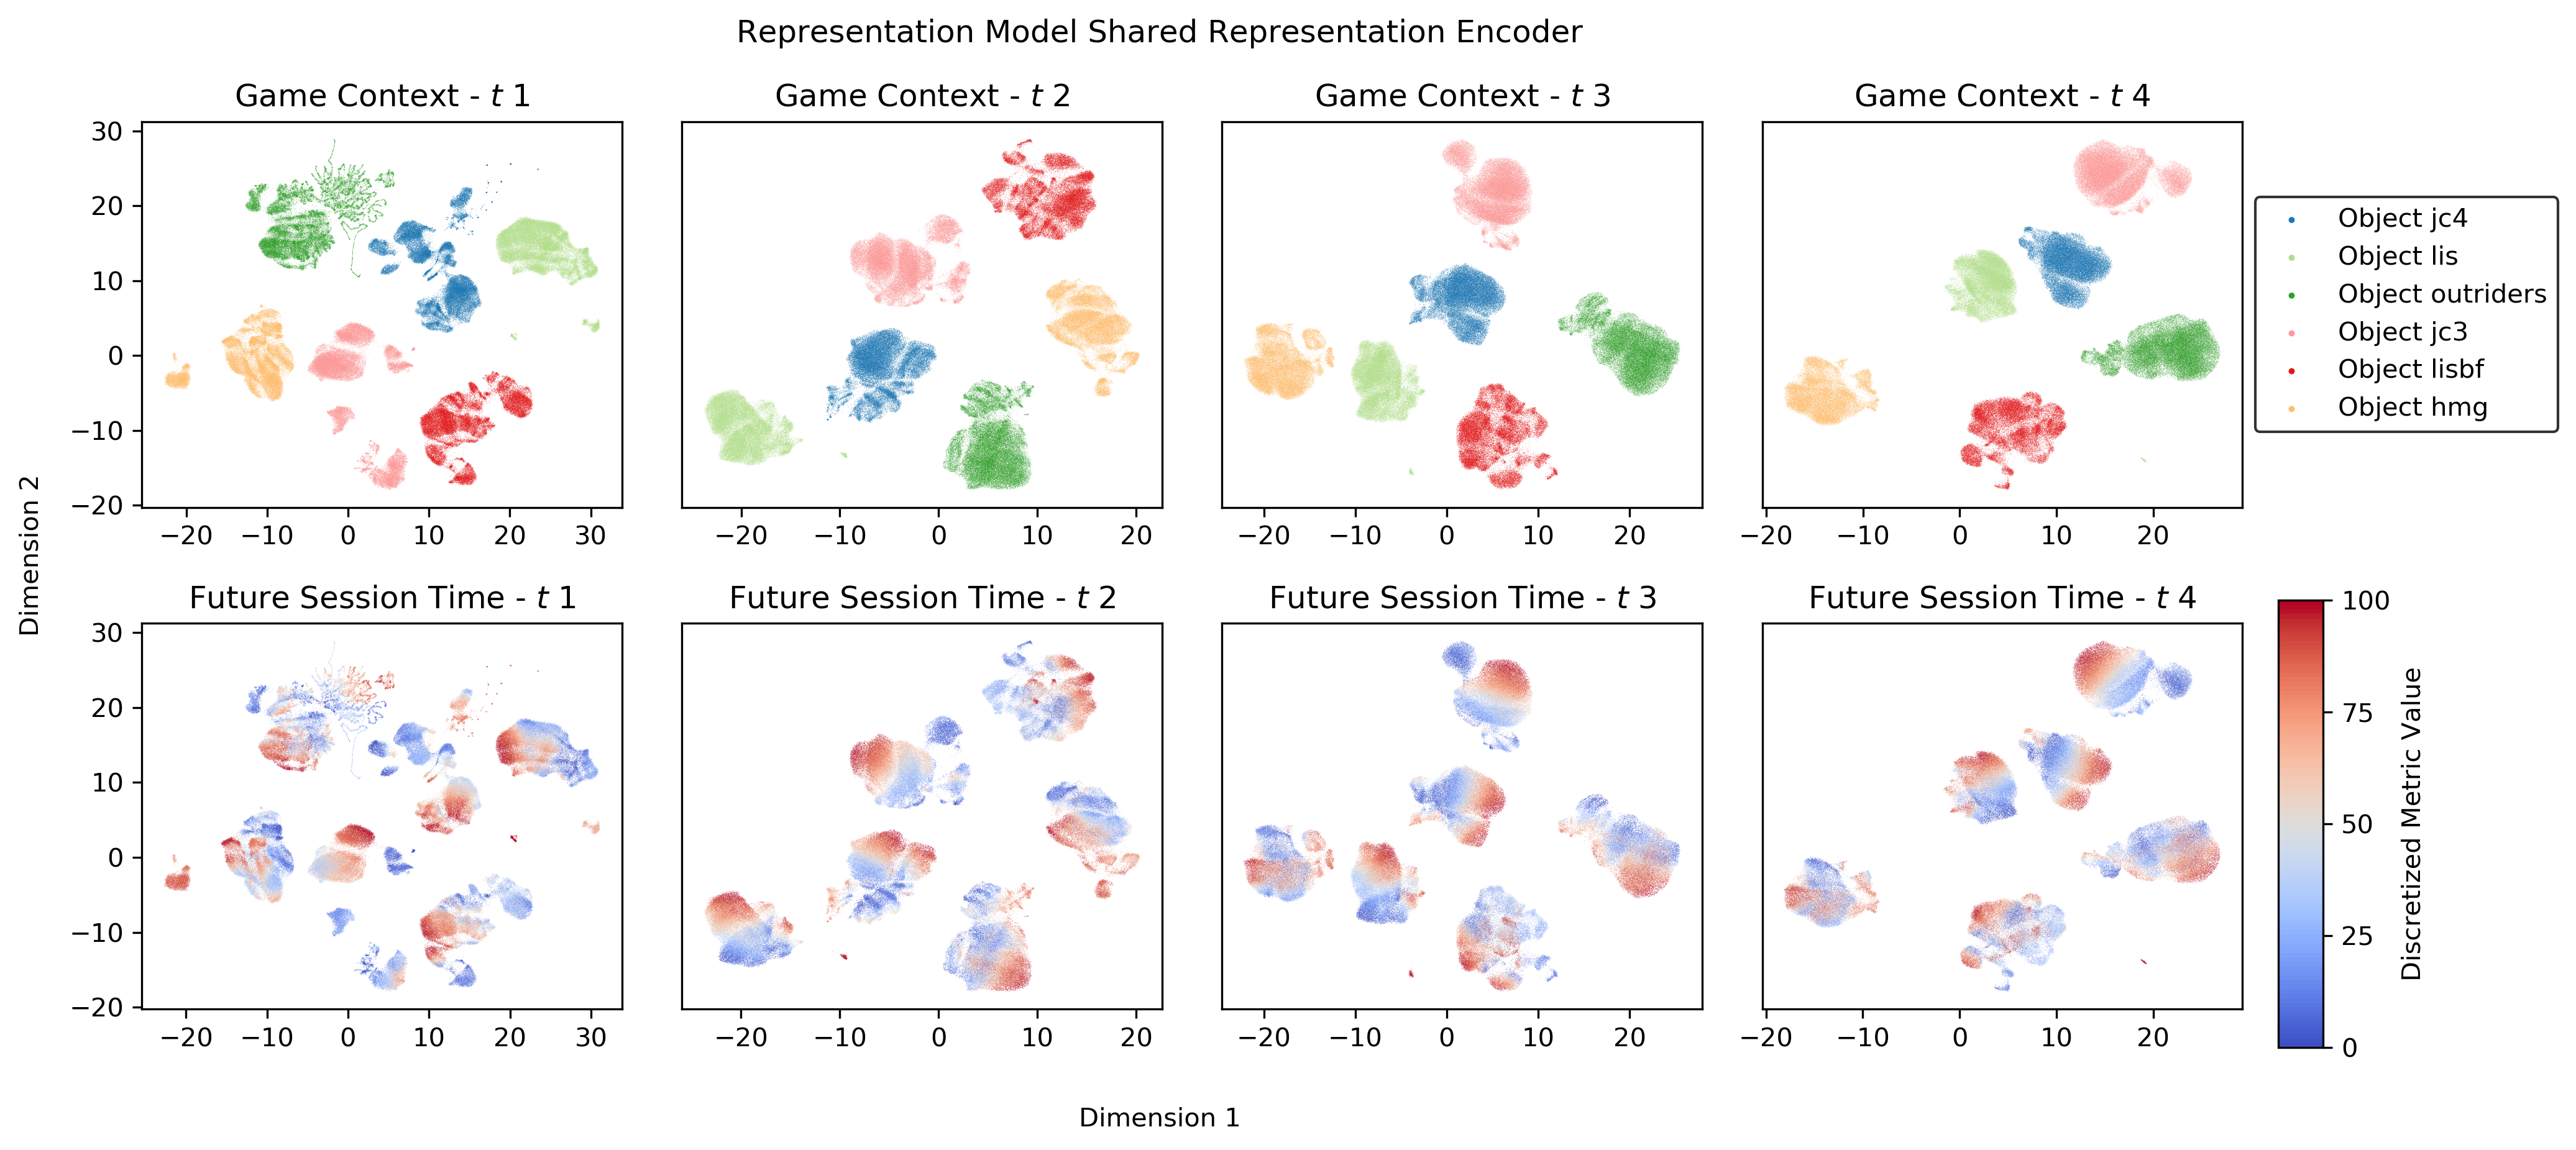
\includegraphics[width=\textwidth]{images/chapter_4/RNN_env_even_0_lstm_layer_shared_Future Session Time.png}
\caption[\textbf{Lower dimensional representation of the shared latent representations generated by the improved version of the RNN architecture}]{Each panel show a two-dimensional projection of the multi-dimensional representation inferred by the improved RNN architecture at $t1$, $t2$, $t3$ and $t4$. The representation presented in this figure has been generated by the portion of the architecture receiving as inputs the representations associated with the behavioural, environmental and game events input and is the one hypothesized to approximate the manifold structure of attributed incentive salience. As in Figure \ref{full_panel_temporal}, x and y axes are dimensions individuated by the UMAP algorithm and can be interpreted as a coordinate system where proximity represents similarity between points. Colours in the first row indicate which game object the representation is coming from while those in the second row indicate the discounted sum of future predictions for a single target (i.e. "Future Session Time").}
\label{rnn_env_even_full_shared}
\end{figure}

This qualitative improvement can be better appreciated when comparing the representation generated by the two version of the RNN architecture, color coded using the ground truth values rather than the predictions provided by the models. Looking at Figure \ref{rnn_predictive_comparison}

\begin{figure}[ht]
\centering
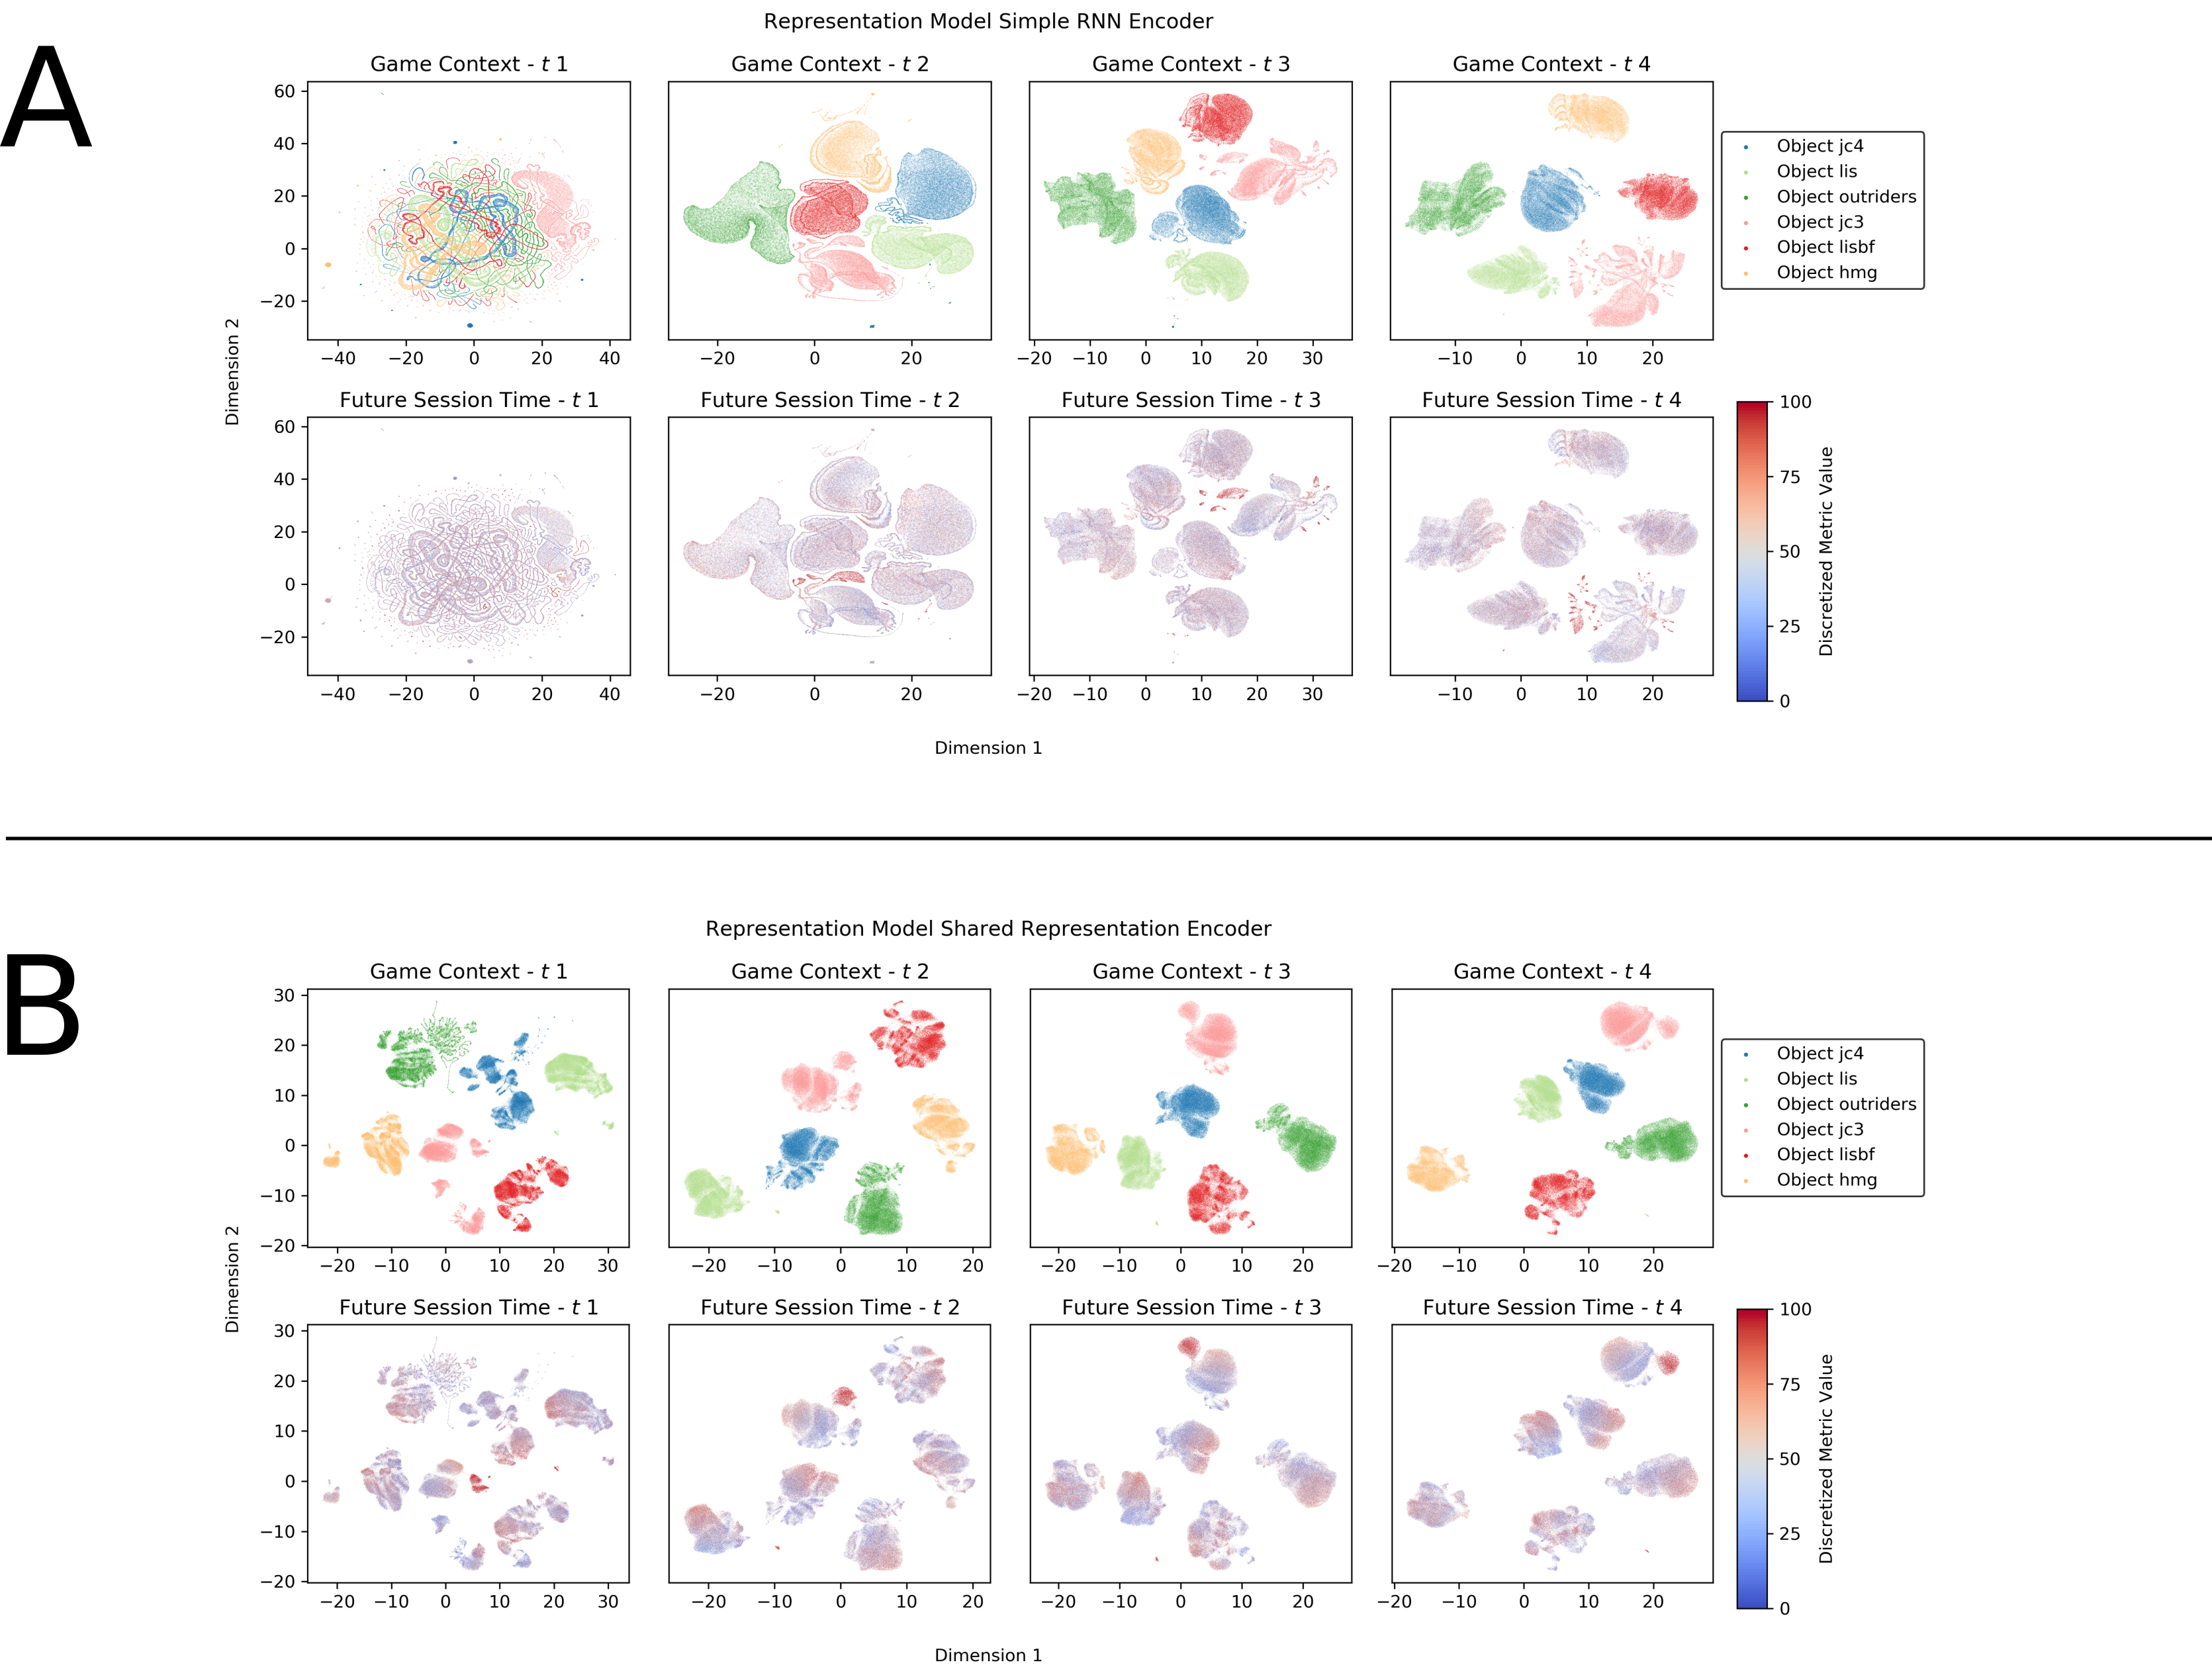
\includegraphics[width=\textwidth]{images/chapter_4/rnn_predictive.png}
\caption[\textbf{Differences in predictive power between the representations generated by the RNN architecture and its improved version}]{The figure show the two-dimensional projection, produced by UMAP, of the multi-dimensional representation generated by the RNN architecture and its improved version at $t1$, $t2$, $t3$ and $t4$. Both representations have been extracted by the portion of the architecture hypothesized to approximate the manifold structure of attributed incentive salience. Panel A refers to the RNN architecture while panel B to its improved version (including environmental and game event covariates). As in Figure \ref{full_panel_temporal}, x and y axes are dimensions identified by the UMAP algorithm and can be interpreted as a coordinate system where proximity represents similarity between points. Colours in the first row indicate which game object the representation is coming from while those in the second row indicate the discounted sum of future ground truth values for a single target (i.e. "Future Session Time").}
\label{rnn_predictive_comparison}
\end{figure}

we can see how the simplified RNN architecture shows a greater level of disruption in the gradient like organization than its improved version, suggesting that this last one is likely to be a better approximation of the functional properties of the latent state (i.e. the level of attributed incentive salience) that generated the observed behaviour. By looking at figure \ref{rnn_env_even_full_shared}, we can notice how the topological characteristics of the previous three representations are replaced by the global-local organization that we described in \ref{functional_properties}. This consistency corroborates the idea that this type of organization is the most suitable one for the type of predictive task that the two architectures are aiming to solve.

\section{Partition Analysis}
\label{partition_analysese}
In order to gather additional insights on the functional properties of the representations generated by our architectures, we attempted to map what inferred by the models back to the observable behavioural space. As specified in section \ref{manifold_learning} these representations are derived from the input metrics and can be interpreted as coordinates on the manifold structure inferred by the architectures. In this view, partitioning them allows identify areas of the manifold holding information about the history of interactions between an individual and a given video game object. Moreover, since the manifold is constructed to be informative of the intensity of future interactions, different partitions might represent not just variations in the input metrics (e.g. differences in the sequences of events triggered in the game) but also in the level of attributed incentive salience. By individuating the set of metrics that contributed to defining the topology of different regions of the inferred manifold we may hope to gather insights on their role in determining the intensity of future behaviour. 

To perform the mapping, we opted for an unsupervised approach and conducted a partition analysis on the representations extracted by the different encoders. 
To partition the data, we decided to apply Mini-Batch K-Means \cite{sculley2010web}, a variation of K-Means, to the representation extracted by the three encoders mentioned in section \ref{representation_analysis}. Given a dataset, the algorithm attempts to divide it by iteratively moving $k$ centroids so as to reduce variance within each partition. The choice of Mini-Batch K-Means was dictated by the fact that it is one of the few distance-based algorithms that scales to very large datasets. The reason for choosing a distance-based algorithm can be found in paragraph \ref{manifold_learning}, there we specified how distance in the manifold structure inferred by an ANN can be interpreted as a measure of similarity between its input with respect to the objective function that the model is trying to minimize. 

To select the optimal $k$ value, we first fitted the algorithm with a varying number of centroids (i.e. 2 to 10) and computed the associated inertia, a measure of within cluster variance (see \ref{inertia}. Since inertia tends to zero as $k$ approaches the number of points in the dataset, we defined the optimal number of partitions as the value of $k$ at which the inertia reached its "elbow" or maximum curvature \cite{satopaa2011finding}. This allows us to identify the point at which increasing the number of partitions provides diminishing returns in terms of within cluster variance reduction. Despite the fact that this procedure might be prone to errors or imprecision (e.g. the elbow might be non-unique or change depending on the maximum number of considered centroids) we thought it would be preferable to an arbitrary choice. 

Every instance of Mini-Batch K-Means was initialized 3000 times at random and ran for a maximum of 3000 epochs. The input data were re-scaled to have zero mean and unit-variance and passed to the algorithm in random batches of size $(512 \times h)$. The associated behavioural profiles were found by applying this methodology separately to each game object and retrieving, for each partition, the expected deviation of all the behavioural metrics from their relative mean (computed along the temporal dimension) in each game context. In order to have an indication of the quality of the individuated partitions, we decided to computecomputed the average silhouette score (see appendix \ref{silhouette}). The silhouette score can be interpreted as an index of cluster cohesion. It is bounded between -1 and 1 and a high value indicates that, on average, all the considered points are well matched to their own partition and poorly matched to neighboring partitions, while the reverse is true for low or negative values. 

We will first focus on inspecting the partitions derived from the representations generated by encoding the behavioural metrics using the RNN architecture and its improved version. We will subsequently move onto the partitions associated with those representation related to environmental and game events covariates. When analysing the obtained partitions we will focus only on those related to the game object $outriders$, results related to other game objects will be reported in appendices \ref{partitions_behavioural}, \ref{partitions_environmental} and \ref{partitions_game_events} and mostly used for drawing general remarks. 

The Mini-Batch K-Means implementation used for this analysis was provided by the python library scikit-learn \cite{scikit-learn}. All the analyses were conducted using Python programming language version 3.6.2 \cite{10.5555/1593511}.

\subsection{Partitioning the representation associated to the behavioural inputs}
\label{partition_behaviour}
As we can see from Figure \ref{partition_rnn_behaviour}, following the methodology outlined in section \ref{partition_analysese}, among all the Mini-Batch K-Means runs, the one with $k=4$ was identified as the optimal one for both representations. All the partitions were associated with a distinct behavioural profile, each one with its own offset and temporal evolution. It is relevant to note that the profiles identified for the two representations are virtually identical (apart from small variations in some of the metrics). However the representation extracted by the improved version of the RNN architecture appears to allow for qualitatively superior (i.e. more compact) partitions as highlighted by the higher average silhouette score.

\begin{figure}[!htb]
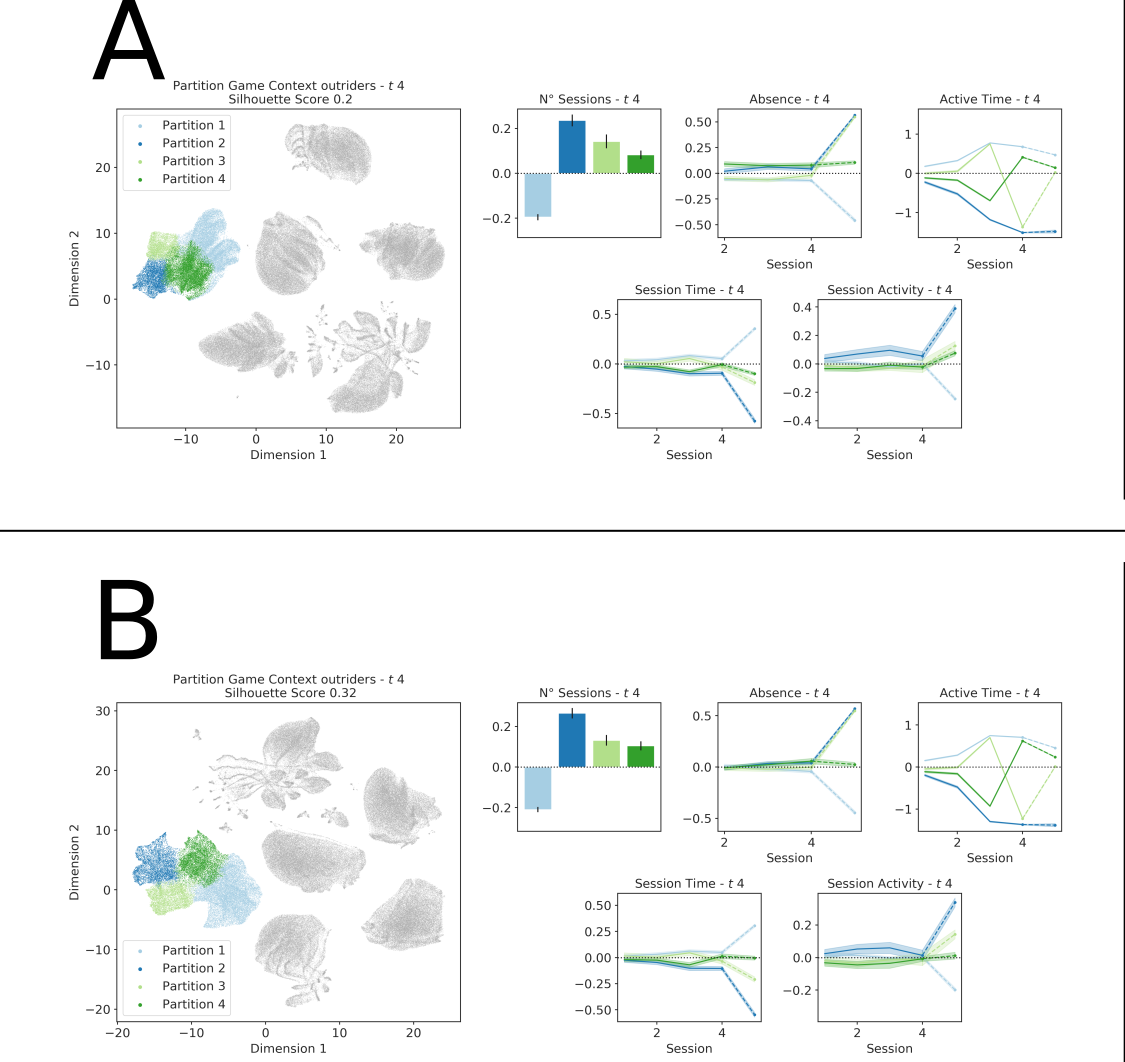
\includegraphics[width=0.7\textwidth]{images/chapter_4/clust_beha.png}
\centering
\caption[\textbf{Partitions of the representations generated by the RNN architectures from the behavioural metrics}]{The two panels shows the individuated partitions and associated behavioural profiles at $t4$. The big panels report the same UMAP reduction presented in the last column of Figure \ref{full_panel_temporal}. Each dot is the representation associated with a particular individual and is colour coded based on the partition to which it belongs. Small panels represent the temporal evolution of the considered behavioural metrics for each individuated partition. The panel showing  N°Sessions only reports the prediction produced by the model as the number of preceding session is constant for all the partitions. The x axis reports the game sessions while the y axis the value assumed by the considered metric at a specific point in time. The y axis is expressed in terms of number of standard deviations from the game population mean (i.e. z-scores). Each line indicates the mean z-score while the shaded area around the line its 95\% confidence interval. The solid part of each line indicates the portion of the temporal series observed by the model (i.e. the input) while the dotted part the predictions produced at that point in time. The first columns shows the partitions associated with the representation extracted by the RNN architecture while the second those associated with the representation extracted by the version of the RNN architecture that included environmental and game events covariates. Each row indicates the partitions identified for the six considered game contexts.}
\label{partition_rnn_behaviour} 
\end{figure}

At a global level, the four partitions seem to belong to two general groups: a group with a high propensity to produce future interactions (i.e. partitions 1 and 2) and a group with low propensity (partitions 3 and 4). Noticeably, when looking in detail at each specific partition they appear as variations on the macro group they belong to. Interestingly the percentage of Session Time spent actively interacting with the game object (i.e. Active Time) and the expected N°Sessions seem to be a relevant components in this more granular characterization. 

We will now report examples of the type of behavioural "phenotype" that we were able to derive from the partition analysis. However, Given the unsupervised nature of the adopted methodology and the lack of any strong a-priori expectations on the profiles' outlook, we suggest to interpret them with cautions and consider them as the result of a purely exploratory analysis.

\paragraph*{\textbf{Partition 1}} represents individuals producing high intensity interactions (see Session Time) at a high frequency (see Absence). The high amount of Active Time highlights how the individuals were actively interacting with the game object. The individuals in this partition are projected to produce a number of future interactions that is below average while maintaining a high intensity profile. It can be speculated that the history of high intensity interactions reflected a positive propensity towards the game. This might have prompted individuals in this partition to consume most of the available contents in the game leading to a reduced amount of expected future interactions (i.e. N° Sessions).

\paragraph*{\textbf{Partition 2}} describes individuals that have a history of very infrequent (see Absence) and brief interactions with burst of activities and long idle times (they have the lowest Active time among the individuate partitions). These individuals are expected to maintain this trend in the future although producing a number of interactions that is largely above the average. An hypothetical explanation might see individuals in this partitions constituting a variant of those in Partition 1. The high frequency and intensity of interactions could suggest an eagerness to interact with the game object. This, combined with the low amount of consumed content (see Session Time and Active Time) could explain the projected high amount of future interactions.

\paragraph*{\textbf{Partition 3}} includes individuals whose interactions have been very frequent and average both in terms of length and amount of activity until session 3. From there, a burst in both the length and active time can be observed concomitant with a reduction in latency before the following interaction. This is followed by a re-bounce effect with a marked reduction in the length and intensity of the next interaction. These individuals are predicted to produce a number of future interactions slightly above average while also maintaining a low intensity profile. These individuals might have started with a normal propensity towards the game which suddenly increased around session 3 and had a "physiological" downturn around session 4. 

\paragraph*{\textbf{Partition 4}} contains individuals producing the least intense and frequent interactions. With the only exception of a brief increase in active time around session 4. These individuals are estimated to produce a number of future interactions just above average while maintaining the original low intensity profile. These individuals started and maintained a low intensity profile, suggesting a negative propensity toward the game. 

It is interesting to note that despite the fact that the partitions identified for the various game objects always show the two "macro groups" mentioned above, their finer grain characterizations (i.e. the behavioural profiles extracted from the partitions) vary between game contexts suggesting the presence of a possible interaction (see Appendix \ref{partitions_behavioural}).

Although the individuated profiles can provide valuable information on the behavioural "fingerprint" of group of individuals, the most relevant and reliable information can be found in the relationship between the considered metrics. We observe that Session Time and Session Activity are usually highly correlated. Low Absence seems to be a good indicator of the propensity to produce more interactions in the future. Similarly, high Absence seems to be associated with a general history of low intensity interactions. It is also worth noting that variations in this metric seem to follow and be proportional to increases and decreases in interactions' intensity. 

We can also notice how there is often (but not always) a very high correspondence between the profiles associated with the representations generated by the two versions of the RNN architecture. However, looking at the average silhouette score values, it seems that including environmental and game event covariates helps to generate tighter and more consistent partitions. This might have been driven by mechanism similar to one that we find in conventional linear models: by including appropriate covariates it is possible to obtain more reliable and robust estimates of a specific coefficient of interest \cite{gelman2020regression}.

\subsection{Partitioning the representation associated to the environmental covariates}
\label{partition_environment}
Looking at Figure \ref{partition_rnn_env} we can see the partitions individuated by the Mini-Batch K-Means for the representation generated from the environmental metrics. Given that all the entries included in our dataset were logged using the same time zone (i.e. CEST) we decided to focus in this analysis only on individuals playing from Central European countries. By looking at Figure \ref{partition_rnn_env}A we can observe how individuals tend to distribute their interactions with a game object differently depending on the day of the week or the hour of the day. This finding is not surprising but is in line with the idea mentioned in sections \ref{estpred_motivation_engagement} and \ref{modelling_env_and_game_elements}: the environment in which an interaction (here, between an individual and a game object) occurs help to determine its observed behavioural intensity. 
\begin{figure}[!htb]
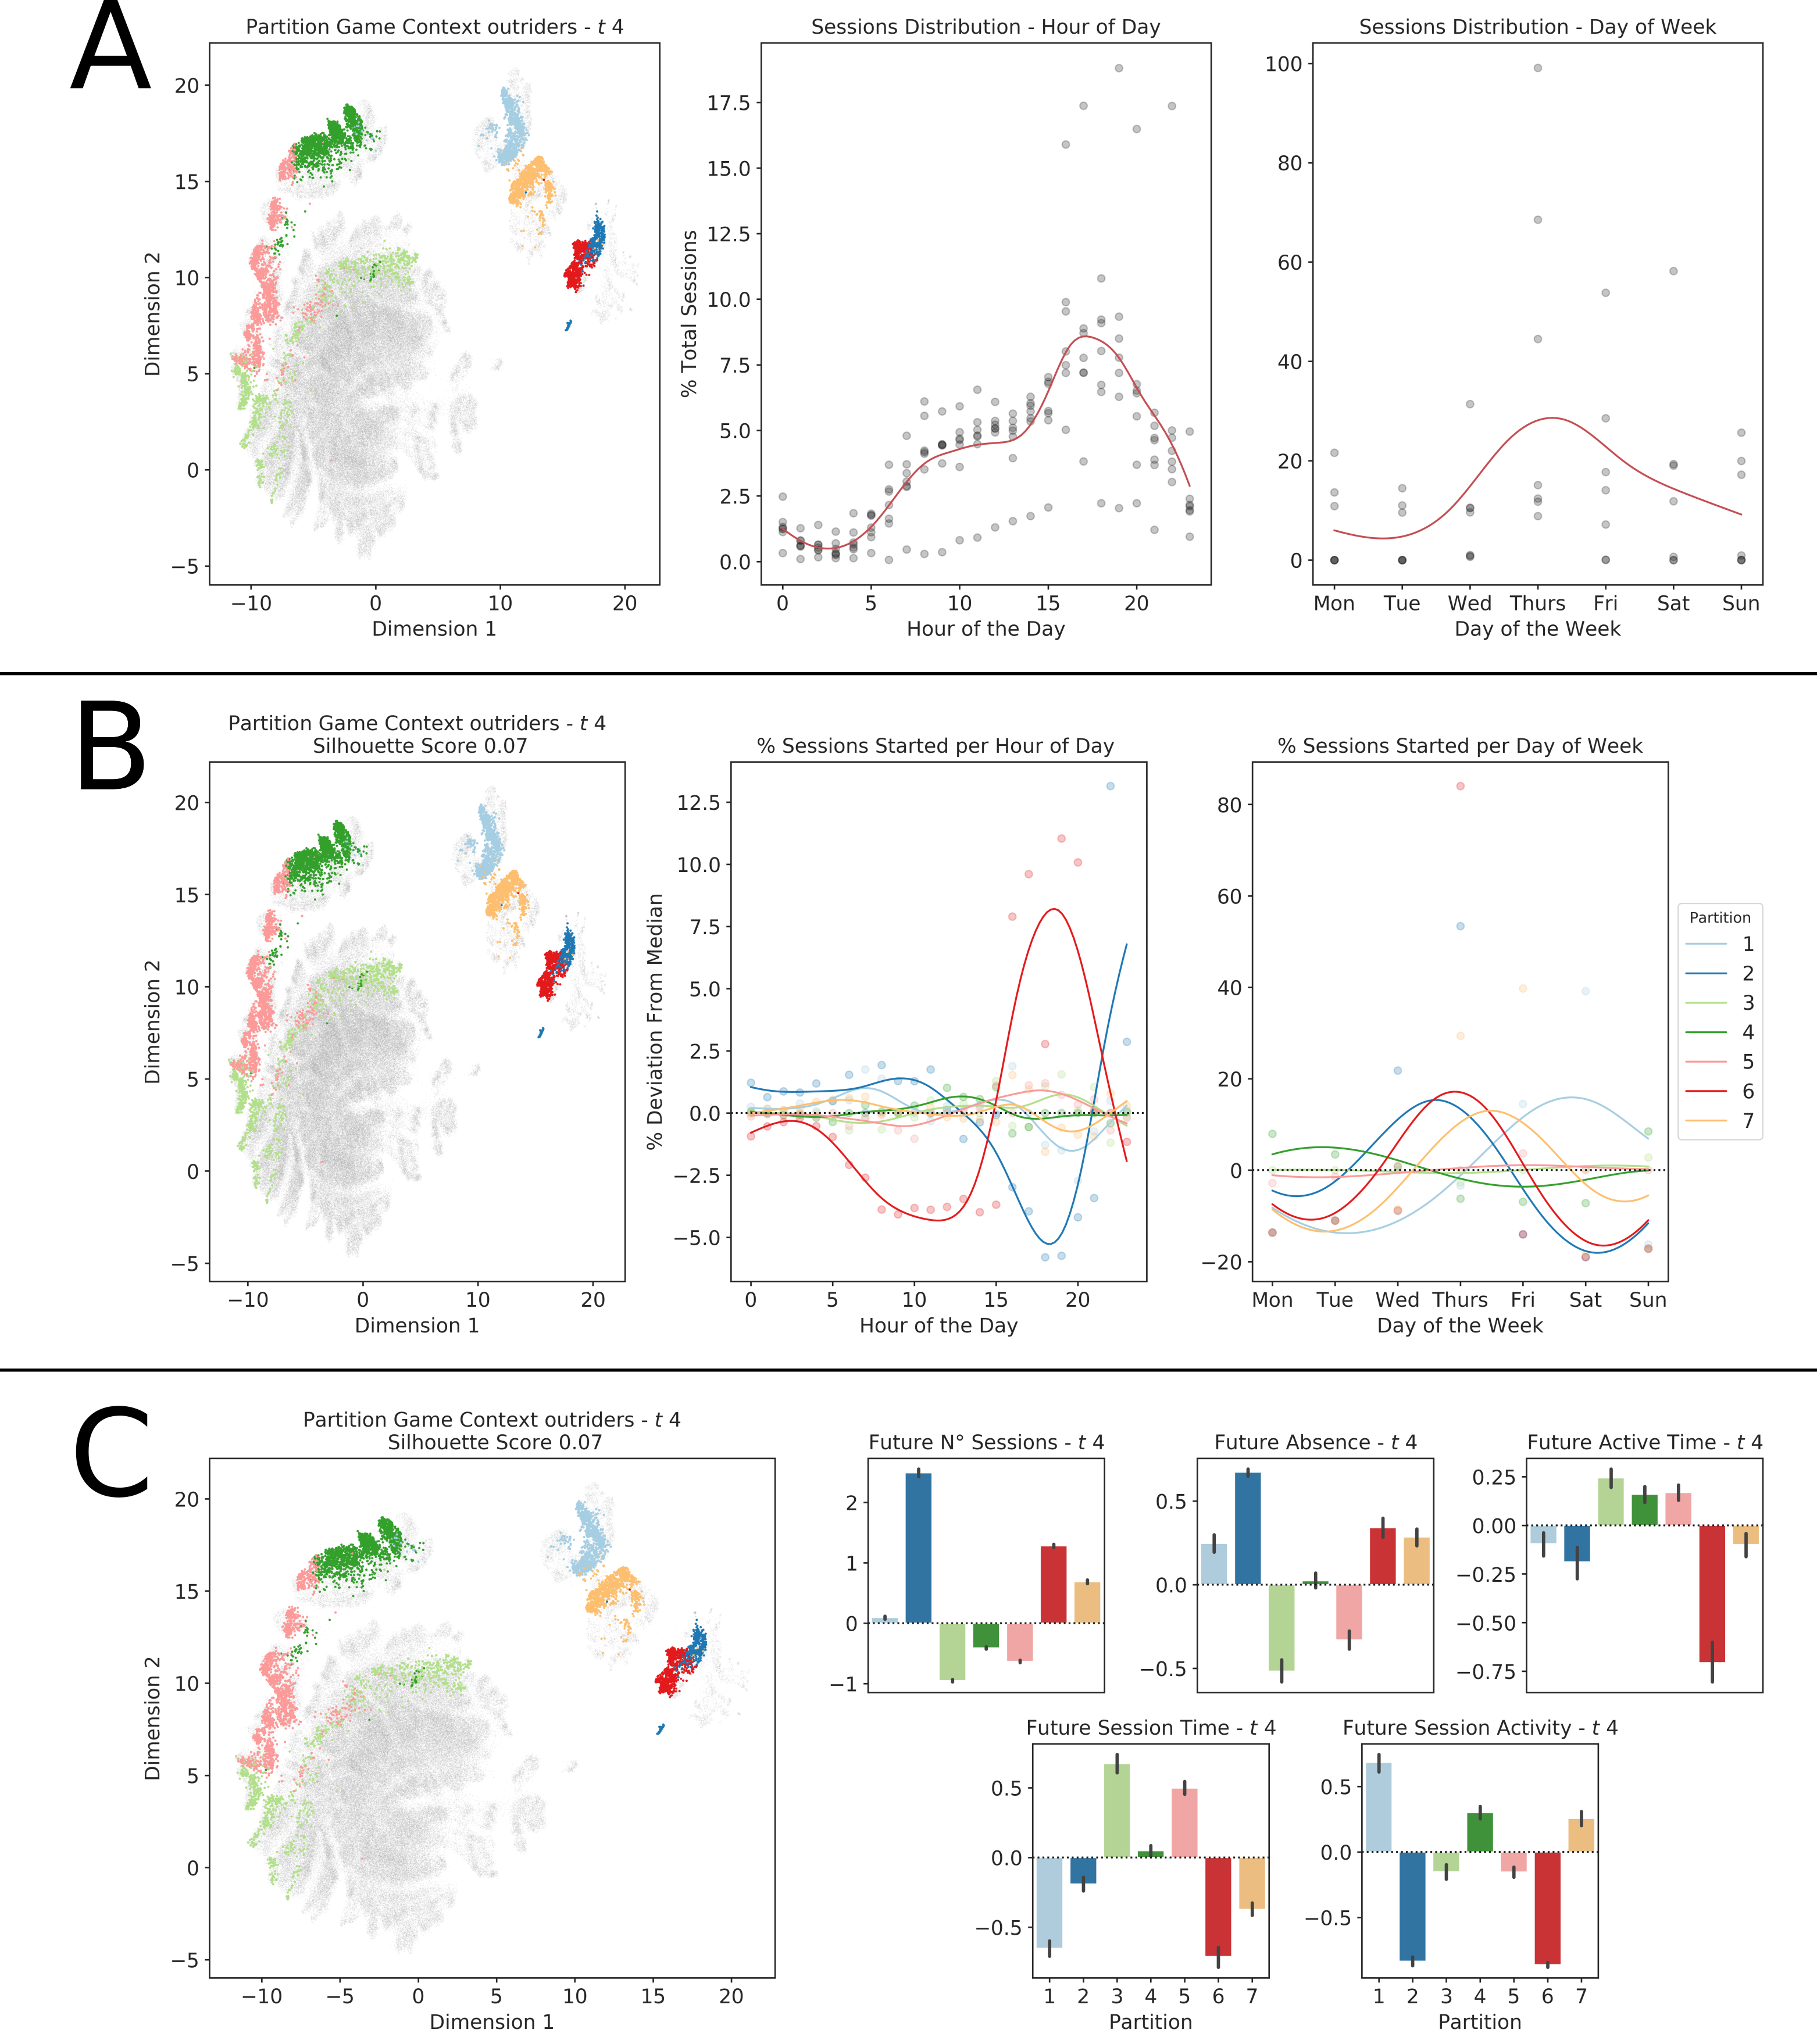
\includegraphics[width=\textwidth]{images/chapter_4/clust_env.png}
\centering
\caption[\textbf{Partitions of the representations generated by the RNN architectures using the environmental metrics}]{The panels show the individuated partitions and associated profiles for the representation encapsulating all the environmental information up to $t4$. Each panel shows the conventional UMAP reduction of the inferred latent representation with the colours representing membership to a specific partition individuated by the Mini-batch KMeans. The other two plots in panels A and B represent the percentage of total sessions that each partition initiated during a specific hour of the day or day of the week. The x axis reports either the hour of the day or the day of the week while the y axis the share of initiated sessions. For each panel we reported the line of best fit provided by a generalized additive model \cite{serven2018}. Panel A shows how each partition distributes its game sessions between different parts of the days or days of the week while panel B provides the same information at the sample level integrating over all partitions. The y axis in panel A is expressed in number of standard deviations from the sample mean. Panel C shows, similarly to Figure \ref{partition_rnn_behaviour} , differences in the predictions produced by the model for each partitions. The x axis indicates the partition number while the y axis the expected prediction made for a specific partition. The y axis is expressed in terms of number of standard deviations from the sample mean (i.e. z-scores) with black line indicating the 95\% confidence interval}
\label{partition_rnn_env} 
\end{figure}

Looking at Figure \ref{partition_rnn_env}A we can observe that the amount of playing activity in the considered sample tends to grow monotonically (but not linearly) from early in the morning (roughly around 6 a.m.) until early in the evening, peaking at around 7 p.m. A finding that is compatible with the expected daily schedule and circadian rhythm of individuals in the considered regions \cite{vitaterna2001overview} and with the results obtained by Vihanga and colleagues \cite{vihanga2019weekly}. A similar pattern can be observed for the distribution of playing activity during the days of the week: starting from Monday, individuals seem to progressively initiate more game sessions over time with peak activity recorded between Thursday and Friday. 

Interestingly, it appears that the nature of the object (i.e. the game context) plays a role in determining how different environmental factors influence the intensity of the interactions. A finding that is in again in line with the work of Vihanga and colleagues \cite{vihanga2019weekly, wannigamage2021player}. Looking at the Figures in Appendix \ref{partitions_environmental}, we can see for example that the game object $hmg$ shows a different distribution of play sessions during the hours of the day with respect to $outriders$. For $hmg$ sessions seem to be roughly equally distributed during the day while for $outriders$ they peak towards the end of the day. This might be explained by the fact that being $hmg$ a mobile game, it allows individuals to  more easily initiate playing sessions at any moment during the day. In other words, the considered environmental factors would be posing less constrains on the intention to initiate the gaming activity. This type of differences appear even more pronounced and pervasive when looking at the distribution of playing sessions over the days of the week. 

More nuanced differences appear to emerge when inspecting the profiles derived by the partition analysis. Looking at Figure \ref{partition_rnn_env}B we can see how different groups of individuals distribute their playing activity differently in a way that is not necessarily compliant with what emerged from Figure \ref{partition_rnn_env}A. As in the case of the behavioural profiles we suggest that   these findings should be interpreted with caution and consider them as descriptive rather than prescriptive. 

\paragraph*{\textbf{Partitions 3, 4 and 5}} represent individuals with a distribution pattern which is not radically different from what observed in Figure \ref{partition_rnn_env}A. Partitions 3 and 5 show a slight preference for evening rather than morning interactions while the opposite is true for partition 4 which seems to also have initiated more play sessions at the beginning of the week. They are expected to have a number of future playing sessions below average, but their next interaction is expected to be of moderately high intensity and to occur in a short amount of time. These individuals might have had a regular schedule of relatively long playing sessions that allowed them to consume a considerable amount of in-game content.

\paragraph*{\textbf{Partitions 1 and 7}} include individuals showing a slight preference for early morning rather than evening interactions. Partition 7 appears to have initiated more sessions late in the week (e.g. Thursday and Friday) while partition 1 seems to have favoured the weekend. The profile emerging from the expected intensity of their next interaction appear to be similar for both partitions: a brief but intense session occurring after a relatively long hiatus. These individuals might have had only a relatively narrow window of time for accumulating their playing activity.  Nevertheless they are expected to keep interacting with the game object (see the expected Future N° Sessions) suggesting that, despite the environmental constrains, they might be attributing high value to the playing activity.

\paragraph*{\textbf{Partitions 2 and 6}} are the ones showing the most unusual and extreme patterns. Individuals belonging to partition 2 appear to have initiated most of their session very late at night or very early in the morning avoiding the afternoon and evening. Partition 6 shows the opposite patterns, with playing sessions happening exclusively between late afternoon and early in the evening. Both profiles appears to have logged most of their activity in the middle of the week at the expenses of the weekend. The next session for these individuals is expected to be brief, of low intensity and occurring after a relatively prolonged period of time. However, these partitions encompass individuals that are expected to have the highest number of future playing sessions. This suggest that, similarly to what we observed for partitions 1 and 7, these individuals might have enjoyed the playing activity but the manifestation of their playing behaviour has been hampered by environmental constrains.

The results of this partition analysis, in conjunction with what emerged in sections \ref{results_3} and \ref{representation_env_even_contr} seems to support our intuition regarding the role of environmental covariates in the representation generated by the RNN architecture. 

These type of factors might influence the intensity of future interactions that an individual has with a particular game object. However they act mostly as facilitators or impediments to the observed behaviour (see partitions 2 and 6) rather than inherently influencing the internal state of the individual. 

Indeed, in contrast to what we observe in Figures \ref{rnn_env_even_full_events} and \ref{rnn_env_even_full_beha}, the representation extracted by the environmental encoder appears unable to clearly distinguish between individuals based on the expected intensity of their future interactions. Interestingly, the results of the partition analysis show that the representation is not just noise but can be used for discerning different patterns of interactions. This suggest that despite the fact that the model was able to organize information to capture similarities between interaction patterns, this might not have been crucial for the minimization of the model objective, or at least not in the same way as behavioural and game events covariates showed to be.

The only notable exception to this seems to be when environmental covariates describe unusual and exceptional situations (e.g., partitions 2 and 6). The reason might be that in these cases there is a correspondence between the environmental conditions in which an interaction occurred and the expected intensity of the next one. For example, speculating that individuals in partition 2 might be doing some form of shift work that allows them to play only late at night or early in the morning, it is reasonable to expect their future interactions to be of low intensity. This is because there is a consistent constrain on how much time they can dedicate to the playing activity, regardless of how enjoyable they might find it.

\subsection{Partitioning the representation associated to the game events covariates}
Figure \ref{clust_even_outr} reports the profiles individuated by partitioning the representation derived from the game events metrics for the game context "Outriders". By looking at Figure \ref{clust_even_outr}A we can see that partitioning the representation we  were able to distinguish between individuals based on the dynamics of their interactions with different in-game mechanics. Apart from partition two, which appeared to have a consistent pattern of engagement (i.e., all the available mechanics were triggered in a similar way over time) the other profiles were able to capture temporal variations in the preference of individuals for different in-game mechanics.

Interestingly, the various partitions appear to encode differences in the amount and intensity of expected future behaviour. This suggests that the inferred representation might have grouped individuals based not just on the similarity between the sequences of triggered events but also based on the impact that these might have had on the generation of future behaviour.

\label{partition_event}
\begin{figure}[htbp]
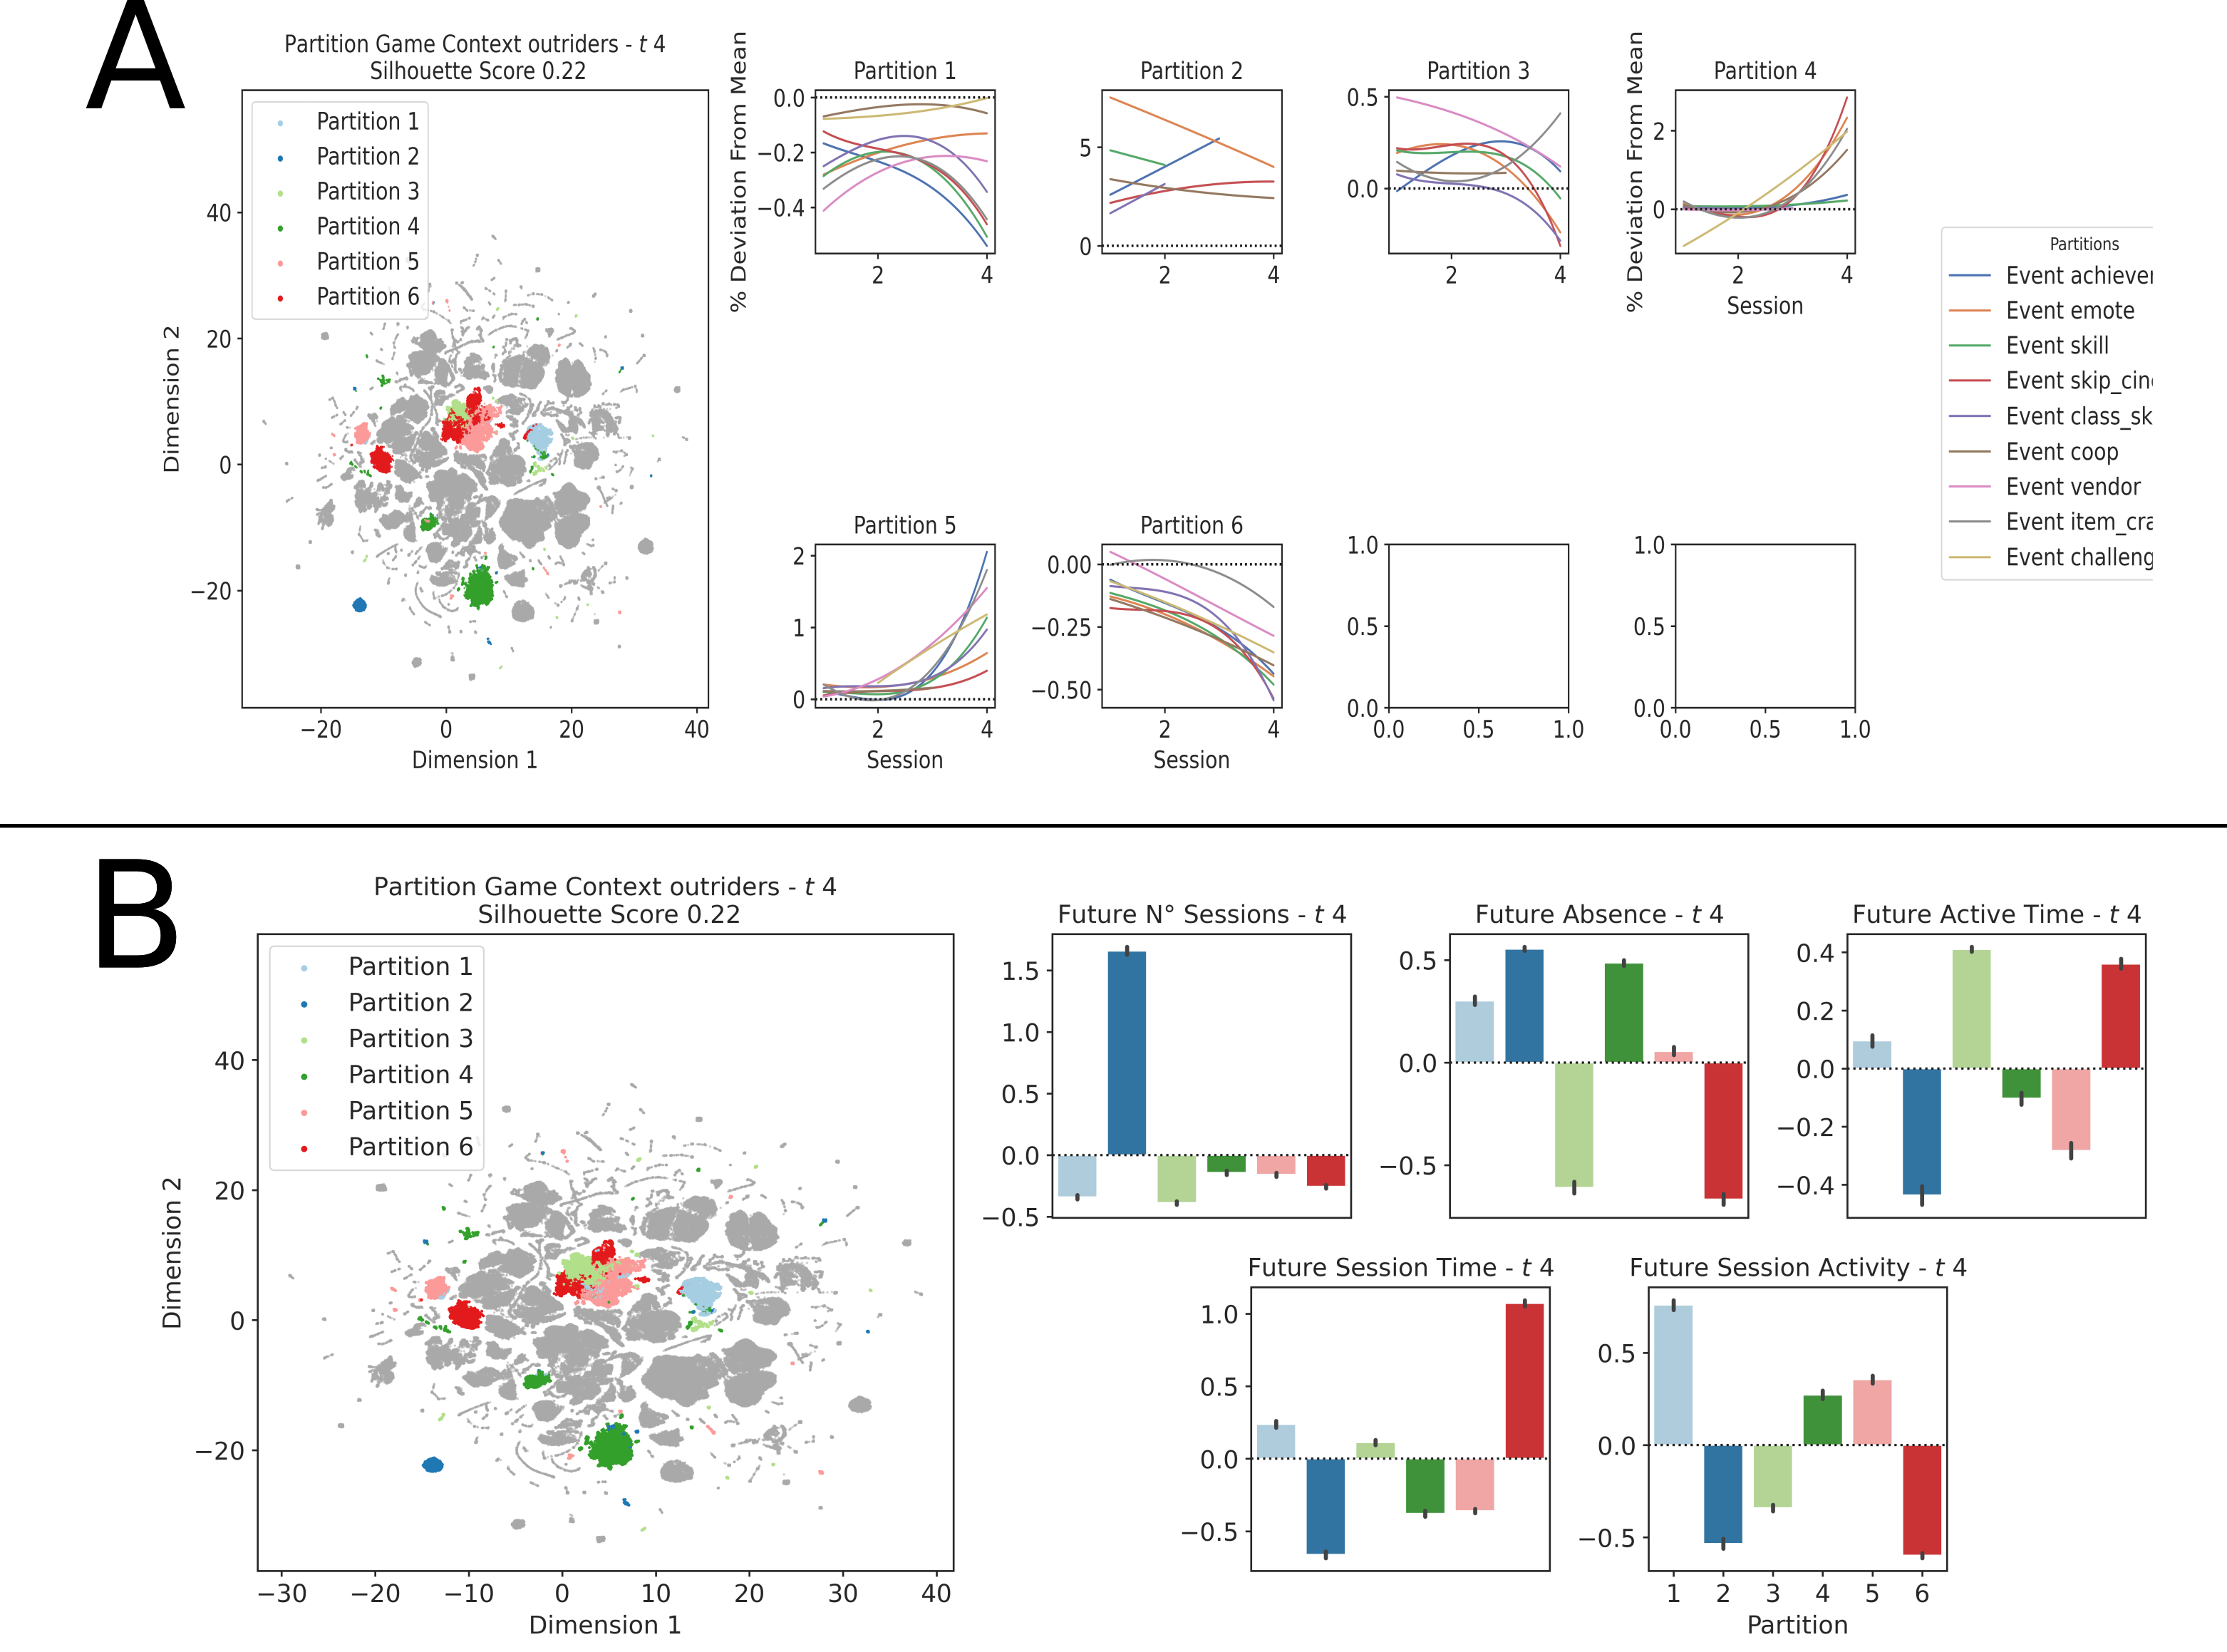
\includegraphics[width=\textwidth]{images/chapter_4/clust_even_outr.png}
\centering
\caption[\textbf{Partitions of the representations generated by the RNN architectures from the game events metrics}]{Panels show the individuated partitions and associated profiles for the representation encapsulating all the game events information up to $t4$. Each panel reports the conventional UMAP reduction of the inferred latent representation with the colours representing membership to a specific partition individuated by the Mini-batch KMeans. Panel A shows for each partition the share of events triggered during each considered game session expressed as number of standard deviations from the sample mean (i.e. z-scores). This information is conveyed through the line of best fit provided by a generalized additive model \cite{serven2018}. Panel C shows, similarly to Figure \ref{partition_rnn_behaviour} , differences in the predictions produced by the model for each partitions. The x axis indicates the partition number while the y axis the expected prediction made for a specific partition. The y axis is expressed in terms of number of standard deviations from the sample mean (i.e. z-scores) with black line indicating the 95\% confidence interval.}
\label{clust_even_outr} 
\end{figure}

\section{Discussion}
As mentioned in section  \ref{incentive_salience}, incentive salience attribution produces latent representations of objects that, when imbued with value, make future interactions with those objects more likely and intense \cite{berridge1998role,berridge2004motivation}. 

The fact that the representation generated by our model could be effectively described by a relatively small number of dimensions (potentially two) appeared to be in line with this and compatible with the idea presented in section \ref{motivation} that motivation-related internal states can be compared to the magnitude of a two-dimensional vector. This metaphor of the "motivational vector" seems to be compatible with the global-local organization of the representation generated by the RNN architecture and its improved version. 

At the global level, different game 'objects' were organized in distinct and coherent regions (see Figure \ref{full_panel_static}A) showing how the model attempted to operate on a meta-level by partitioning a global representation in several object-specific ones. This finding aligns with what highlighted in various work on neural manifold where the responses related to qualitatively different stimuli tends to show a cluster-like organization when reduced to a lower dimensional space \cite{stopfer2003intensity, gallego2017neural, ganmor2015thesaurus}. 

At the local level, each object-specific representation showed an internal gradient-like organization distinguishing individuals based on the estimated intensity of their future interactions with that specific object. This was true for each of the considered behavioural targets (see Figure \ref{full_panel_static}A) showing how the model attempted to provide an holistic description of the intensity of future interactions. The presence of this type of gradient-like organization emerged in work by Nieh et al. \cite{nieh2021geometry} when analyzing neural responses during an evidence accumulation task in virtual reality. When reducing the neural activity to a three-dimensional space, the resulting manifold presented a clear gradient able to code simultaneously for position and levels of accumulated evidence \cite{nieh2021geometry}. A similar finding was present in the work by Stopfner et al. \cite{stopfer2003intensity} where the manifold structure extracted from the activity of olfactory neurons was able to represent qualitative and quantitative differences between odours through a global-local organization similar to that showed in section \ref{functional_properties}.

The dynamic nature of the representation generated by our approach also fits nicely with that of attributed incentive salience \cite{toates1994comparing,robinson1993neural,zhang2009neural,tindell2009dynamic,berridge2012prediction}. In particular, the fact that the aforementioned global-local organization is maintained over time (see Figure \ref{full_panel_temporal}A) corroborate the hypothesis that our model approximated state changes originated from a dynamic process. In support of this, we also observed that the representation generated by our model was spatially coherent over time: it produced distinct regions of low and high expected intensity between which individuals moved over time (see Figure\ref{full_panel_temporal}D). These results appear to match the definition of motivation and incentive salience attribution specified in section \ref{motivation}: a single overarching process able to dynamically predict the likelyhood and intensity by which individuals will interact with a varied set of objects \cite{simpson2016behavioral,toates1994comparing,berridge2004motivation,zhang2009neural}. 

Many other cognitive and affective functions might rely on a latent representation that is functionally similar to the one described in our work (e.g. credit assignment and optimal control \cite{wang2018prefrontal, barto2004reinforcement, friston2012active}, cognitive control, learning \cite{skinner1965science},various forms of reward processing \cite{schultz1997neural, schultz2000reward}). Similar to attributed incentive salience, these functions are all involved in generating motivated behaviour and heavily rely on reward signals, however none of them is concerned with attributing and describing the motivational saliency that an object possess. This is made evident in the works by McClure et al. \cite{mcclure2003computational} and Zhang et al. \cite{zhang2009neural} where the system involved in salience attribution is functionally separate from the one assigning credit and executing actions: the former provide a representation that informs and biases the decisions taken by the latter serving an almost exclusively qualifying role (see the role of attributed incentive salience in addiction-like conditions \cite{robinson1993neural}). Similarly, the representation generated by our model does not provide any insight on the decision making process underlying the observed playing behaviour but simply provide an approximate description of the "motivational pull" that a particular game object has on a particular individual at a certain point in time. 

The functions encoded by the hidden units constituting the representation appeared to have a series of distinctive properties, namely: redundancy, non linearity, multiplicity (single units code for multiple functions) and consistency over time. These may have played a role in providing the representation generated by our model with its distinctive characteristics. For example, as we mentioned in section \ref{manifold_rep_incentive_salience} redundancy and inter-correlation are characteristics of the signals from which the manifold representation of internal states arises \cite{seung2000manifold,gallego2017neural}. Multiplicity on the other hand, might be the factor underlying the ability of our model to produce a single unitary representation which holds predictive power over different behavioural targets. Finally, consistency over time could be the mechanisms supporting the type of temporal coherence observed in panel \ref{full_panel_temporal}D. We want to stress that these findings are to be considered exploratory in nature since they do not rely on \textit{a-priori} hypotheses. A comparison between these computational properties and those underlying the attribution of incentive salience is required and would constitute a potential venue for future investigations. 

The introduction of environmental and game event covariates appeared to have produced a more consistent representation (see Figures \ref{rnn_env_even_full_shared} \ref{rnn_predictive_comparison}) with better discriminatory powers, a finding in line with the, although marginal, improvements in predictive performance observed in section \ref{results_3}. It might be speculated that this improvement was associated both with the introduction of new informative covariates and with the ability of the architecture to separately model their contribution. Indeed, similarly to the idea underlying Neural GAMs \cite{agarwal2021neural}, different portion of the architecture might have focused on inferring specialized functions then combined in a more effective latent representation.

However, the major advantage provided by separately modelling the contribution of behavioural, environmental and game-events metrics lied in the ability to obtain distinct representations that we were able to leverage for exploratory analyses. This allowed us to perform time series partitioning at a much larger scale that has been previously done in the videogames literature (potentially up to millions of time series) \cite{bauckhage2014clustering, makarovych2018like, vihanga2019weekly, aung2019trails}. Indeed, previous approaches in the literature attempted to cluster or partition directly the observable data space, a particularly cumbersome process for univariate and multivariate time series, especially if suitable techniques like Dynamic Time Warping \cite{muller2007dynamic} are to be used. In our case by leveraging the representational power of ANNs we were able to condense the information present in the the time series data to a more compact representation, this allowed us to then rely on relatively inexpensive algorithm (i.e. Minini-Batch KMeans) for performing the partitioning.

The partition analysis conducted on the behavioural representation allowed to individuate a set of profiles that are, to a certain extent, consistent with behavioural correlates of different levels of attributed incentive salience \cite{berridge2004motivation} and general operant conditioning principles \cite{thorndike1927law, skinner1953science, nevin2000behavioral}: the strength of past interactions positively correlate with the frequency and intensity of future ones. The various offsets that each partition showed might suggest different levels of predisposition towards the various game-objects. The dynamic nature of these profiles provided a more granular characterization allowing to observe variations in the entire history of interactions and not just in the expected intensity of future ones. For example, it was possible to see how a higher likelihood of future interactions was supported both by a history of low intensity but high frequency interactions as well as by a series of high frequency and high intensity interactions. In this sense, these behavioural profiles can be seen as useful devices for investigating the existence of inter-individual differences in schedules of interactions with potentially rewarding objects. 

On the other hand, partitioning the environmental representation provided us with insights on how different individuals distributed their interactions with a videogame over days of the week and hours of the day. We were able to replicate some of the findings of Vihanga and colleagues \cite{vihanga2019weekly, wannigamage2021player}, identifying similar profiles of interactions. However, our approach allowed us to gather insights not just on the characteristics of the different profiles but also on their potential impact on interaction intensity. A similar conclusion can be drawn from the partitioning of the game events representation. We were able to identify not just  how different groups of individual distributed their playing activity between different in-game events but also how these evolved over time. Moreover in contrast to the work of Makarovych et al. \cite{makarovych2018like}, our approach did not just identify frequent patterns of interactions with in-games elements but also the associated variations in the intensity of future behaviour.

\chapter{Model Application and Pipeline}
\label{chapter_appliction}
\section{Introduction}
\label{industry_needs}
As we mentioned in chapter \ref{chapter_general_intro}, despite the main aim of this thesis has been to derive a methodology for approximating the motivational state of individuals while interacting with potentially rewarding object (a videogame in this case), a secondary objective was to illustrate the potential application of this methodology within an industrial setting.

In this view, this chapter will focus on sketching the design of a system relying on our methodology for automated engagement prediction. First we will introduce a set of ethical considerations that should be taken into account when designing such system. Subsequently, we will provide an overview on why an industry player (or groups thereof) might need a process for quantifying and predicting engagement and which characteristics this process should have. Finally we will proceed at illustrating a system designed for serving this need, placing particular emphasis on how its components connect with the work presented so far.

\section{Some Ethical Consideration}
\label{ehtical_considerations}
Automated system leveraging behavioural data are now-days used extensively in both low and high stakes scenarios \cite{mehrabi2021survey}, with the potential to have a direct and concrete impact on individuals. For this reason, when designing automated data-driven applications, issues related to fairness should be taken into account. 

By fairness we entail the set of principles and considerations that in recent years are adopted in order to avoid that decisions based on a machine-learned model do not inadvertently bring harm to specific groups of people \cite{mehrabi2021survey}. A complete overview of the issue of fairness in machine learning would be beyond the scope of not just this section but the entire thesis, as it is a vast landscape \cite{mehrabi2021survey} hard to navigate due to its many levels of complexity \cite{corbett2018measure}.  We will therefore focus on three major aspects related to the work presented in this chapter. 

The first aspect concerns biases present in the data on which a machine learning algorithm is fitted. These might be induced by an over or under representation of certain strata of the population that an automated system will ultimately need to serve \cite{mehrabi2021survey}. Given how a large part of machine learning algorithms are fitted to the data (e.g., maximum likelyhood) the risk is that the prediction produced by the algorithm will revert to the mean or in the worst case, will result to be biased with respect to the true characteristics of the population \cite{corbett2018measure, mehrabi2021survey}. Despite the harm that these biases might cause in the context of engagement prediction is not as pronounced as in other areas (e.g., credit, criminal or medical risk assessment), they can still have unexpected repercussion on an individual if they assume that people engage in similar ways regardless of situational, personal and cultural differences. For example an individual might receive notifications in inappropriate contexts (e.g.,  during an emotionally challenging period) or be unfairly penalized within the game world (e.g., due to irregular playing patterns caused by personal or situational reasons) because they deviate from what is the expected behaviour in the data on which the algorithm was fitted.

To this connects the second aspect of fairness that we want to highlight, namely the risk of inadvertently cause harm to individuals which are either temporarily or structurally subject to some form of vulnerability. This might happen as a consequence of automated decision making based on what we call "unconstrained model predictions", what we mean by this is when the predictions from a model are used verbatim without knowing the context in which they will be applied. For example, if we imagine a system aimed at individuating high spending users within a game relying on gacha or loot-box mechanics, relying on unconstrained predictions might in this case inadvertently target individuals with a predisposition to or an history of problematic gambling behaviour \cite{petrovskaya2022prevalence}. The most problematic aspect related of this issue is that often the information required for "constraining" an "unconstrained prediction" are not available to the system, either because they are not easy to derive (e.g., they are not directly observable) or should not be accessible (e.g., they are Personal Identifiable Information - PII \cite{EUdataregulations2018}).

Related to the first two points is the third and final aspect of fairness that we would like to address which is connected with the right to object specified by the General Data Protection and Regulation act (GDPR) \cite{EUdataregulations2018} which allows an individual to object to the processing of their data in any form and at any moment. Despite this aspect is partially attenuated by rights granted by the GDPR (although this interests exclusively the European Union), it only covers the processing of data rather than the effect connected with automated decision making. An individual might object to the inclusion of their data during the decision making process but still be subject to the effect of this last one, for example if the system entails a policy of blanket intervention based on the average user behaviour for all those individuals for which no data are available.

As we mentioned at the beginning of the paragraph, an exhaustive treatment of these issues and the relative mitigating actions that could be taken is beyond the scope of the current work. Nevertheless we want to stress that addressing them in an effective manner is of pivotal importance when automated systems based on machine-learning (or other form of statistical decision making) becomes part of the operations of an industry player.

\section{Autometed Engagement Quantification and Prediction in a Videogame Setting}
\label{industry_needs}
As we mentioned before, in an industry setting the development of research projects often aims at the the resolution of specific problems or at the improvement processes central to its success (being it measure in terms of revenues or perceived quality of goods and services). 

So where does engagement quantification and prediction sits within the needs of the videogame industry? Very often (if not always) the success of a videogame title is strictly connected with either its ability to retain users or with the experience that users had with the product (i.e., a videogame title) \cite{amit2001value, alomari2016mobile}. The first is pivotal in scenarios where games are treated as a service sold to an audience (similarly to the function of streaming services) while the second is more relevant in situations where games are considered digital goods \cite{amit2001value, alomari2016mobile}. 

In this context, engagement can be viewed as a measure of how a particular game was, is or will be able to retain users. For example, if an individual is engaged with a particular service (e.g., a videogame) it is likely that will keep paying a subscription (or any other form of pay-to-consume) for said service. Similarly, if an individual had a good experience with a particular digital good, it is is more likely that will promote it to other potential users, acquire similar products or buy products from the same seller.  

In this view being able to estimate the propensity that a user (or a group of users) has towards a particular game translates (in a more or less direct way) to the capacity of assessing if a game is likely to be a success of public and revenue. For this reason it is often the case that videogame publishers and studios try to leverage the information they have available through telemetry system for taking the stock of how a particular game is performing \cite{el2016game}. 

This is the classical example of analytical reports summarizing various type of Key Performance Indicators \cite{el2016game} or profiling techniques describing how users interacted with a particular game \cite{el2016game}. Despite this approaches are extremely relevant for gathering insights on the perfromance of a particular game title, they only allow to execute what we call "reactive" interventions. By reactive interventions we mean that mitigating actions for improving a sub-optimal situation (e.g., when a videogame is unable to foster engagement) can only be taken \textit{ex-post}.

On the other hand, interventions based on the outcomes of a predictive model are by definition "pro-active". This because by knowing in advance if a particular situation is going to be problematic or not allows to plan and deliver mitigating actions \textit{ex-ante} \cite{el2016game, el2021game}. It is worth noticing that approach based on the outcome of predictive models are not incompatible with techniques used within a "reactive" framework (e.g., reports and profiles) but rather complementary. For example the same KPI calculated on observed data can and should be computed also on predictions and forecast generated by a machine-learned model. Similarly, it is possible to create profiles that not just describe the historical interactions of users with a particular game but that are also informative of the expected future engagement of such users.

Within this last "pro-active" framework lies the work that we presented in this thesis. We will now proceed at illustrating the design of a system aimed at delivering predictions and insights that can to foster \textit{ex-ante} interventions for the mitigation and improvement of videogames engagement.

\section{System Design Diagram}
\label{pipeline}


\begin{figure}[ht]
\centering
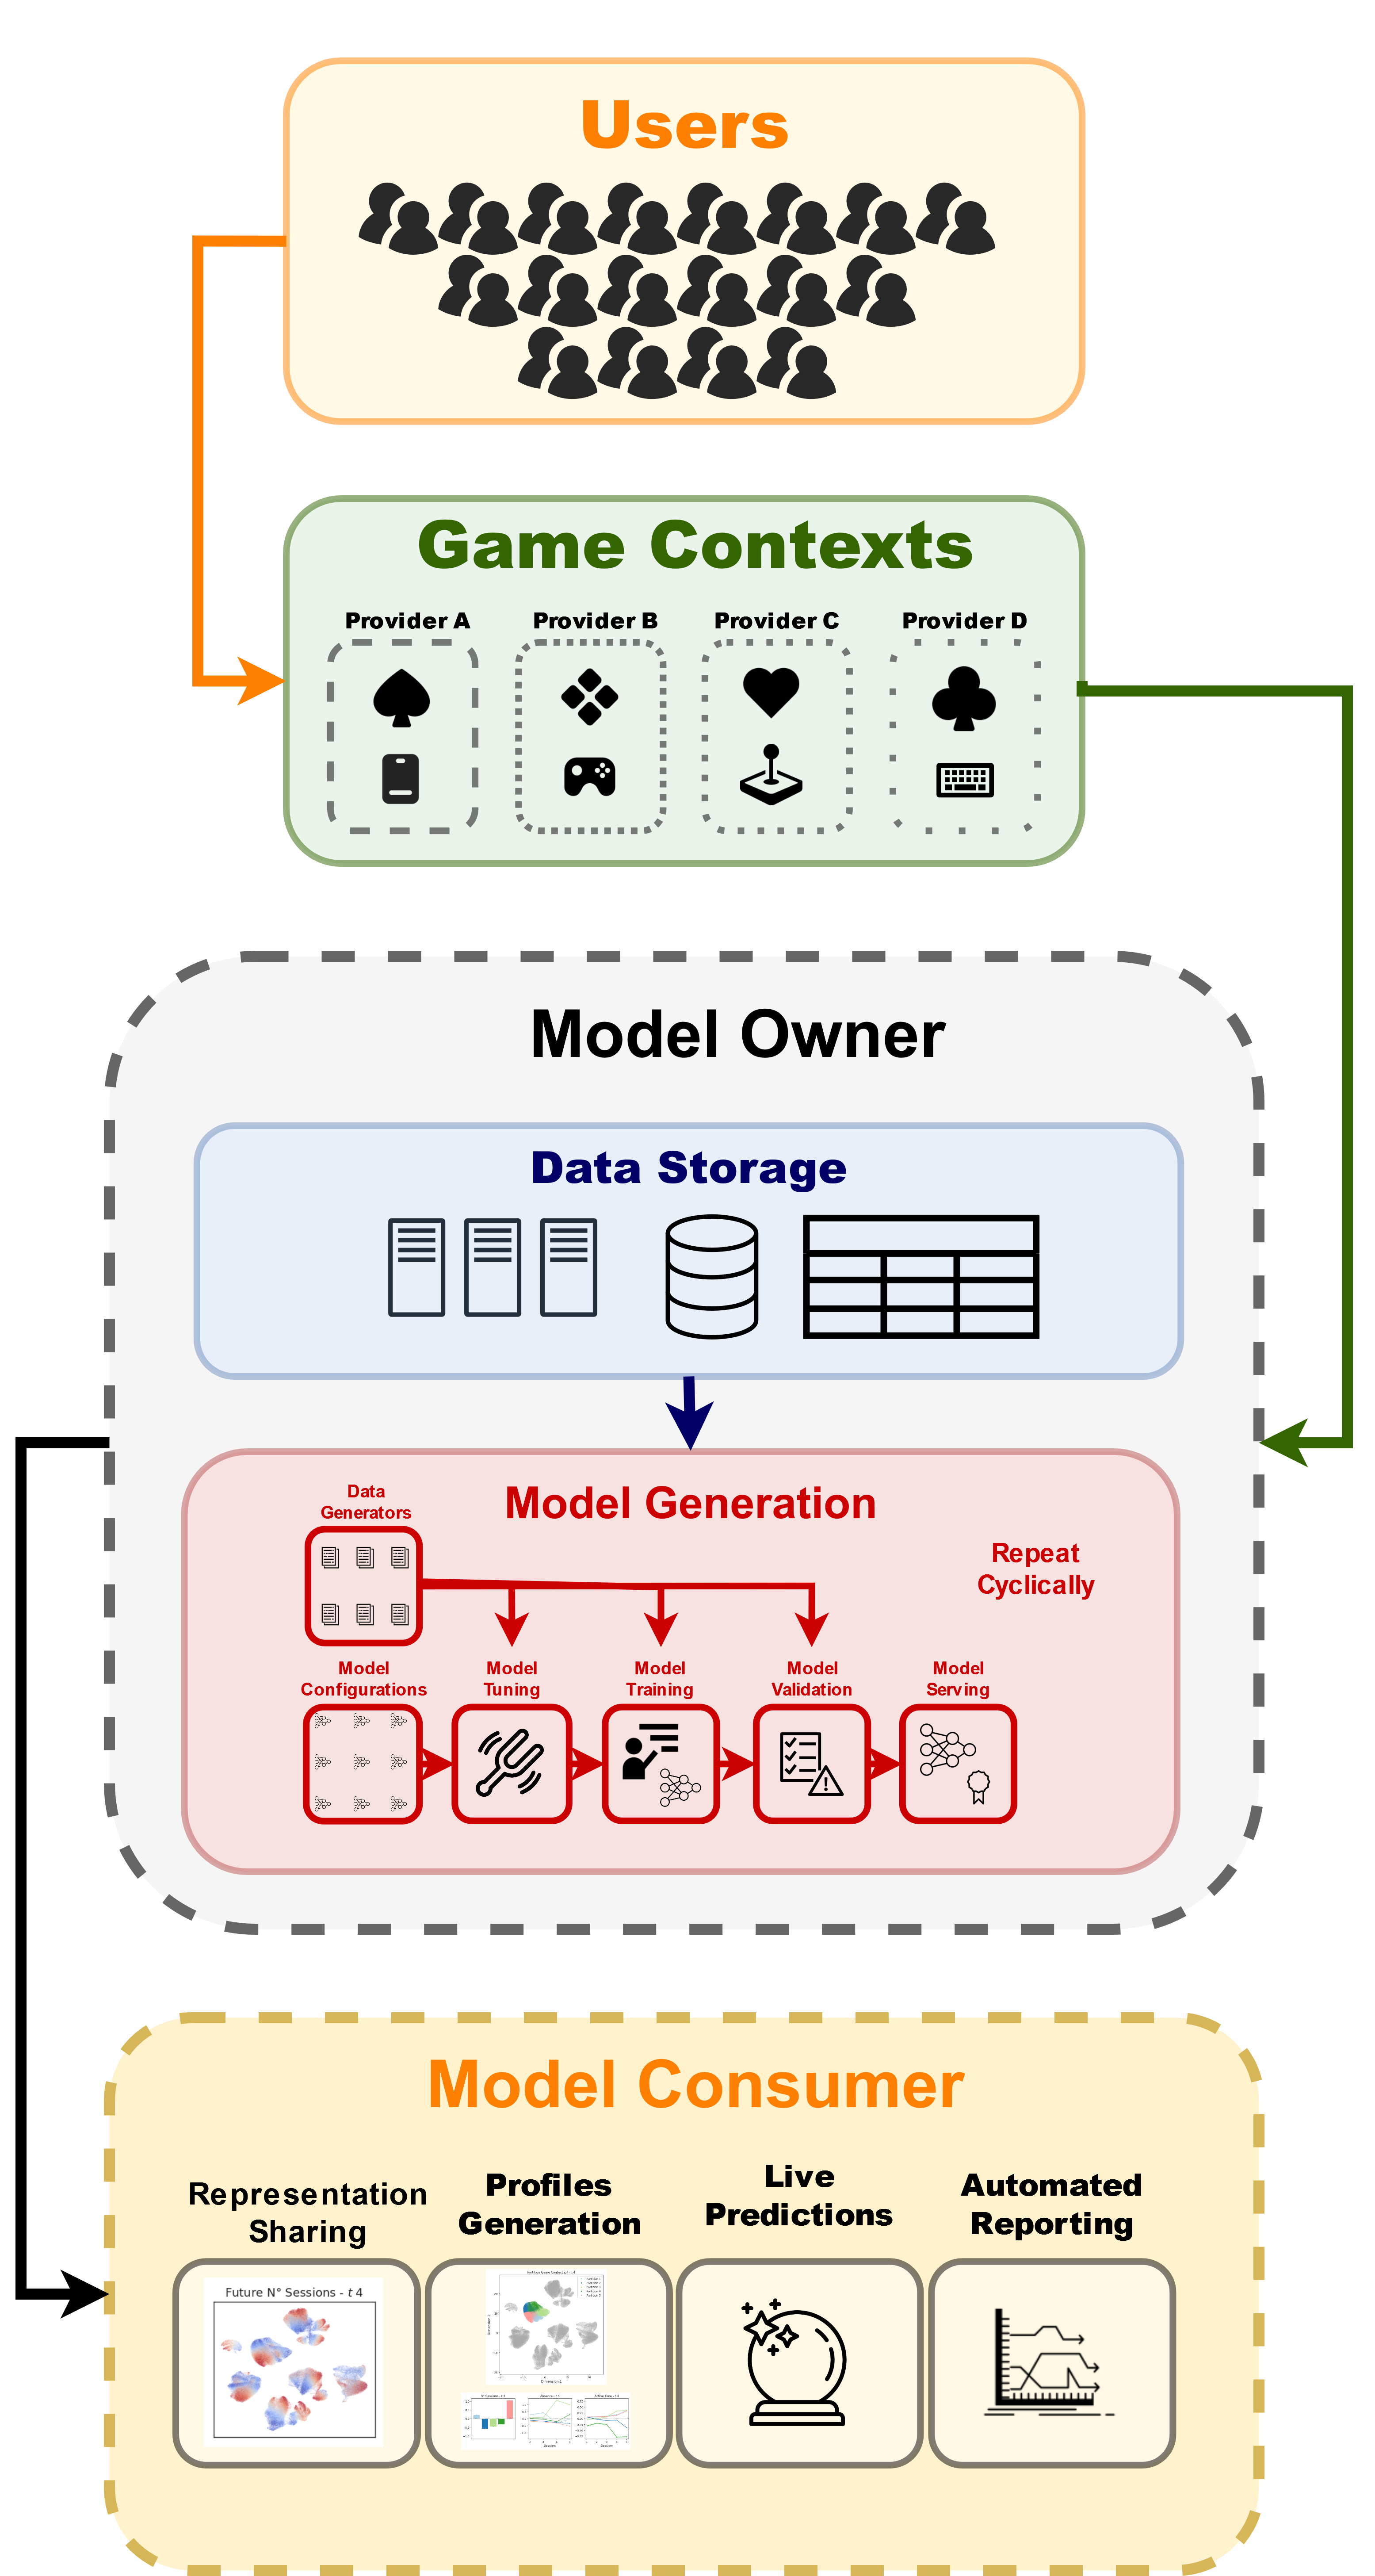
\includegraphics[width=0.7\textwidth]{images/chapter_5/pipeline_diagram.png}
\caption[\textbf{Model Deployment Pipeline}]{The figure represents a simplified system diagram for a potential application of the improved RNN architecture. Solid lines represent low-level components in the system while dashed lines indicate high-level entities. Directional arrows represent the flow of operations inside the system.}
\label{pipeline}
\end{figure}

\section{Data Generation}
\label{data_generation}
This is the first component of the system and describes the entities generating the data that will then be used by the system. It is composed by two major elements: the users and the game contexts. 

The relationship between these two entities has already been described in chapter \ref{chapter_lit_review} and chapter \ref{chapter_theory_modelling} in particular. In line with the framework that we adopted through out this thesis we assume that each game context posses properties (defined by their structural characteristics) that might result more or less rewarding to different users. By means of repeated interactions with the game contexts the users learn about these properties and progressively updates latent representations of the various contexts. These representations, which as we said in chapters \ref{chapter_lit_review} and \ref{chapter_theory_modelling} are imbued with value, act by either promoting or demoting future engagement with the game contexts quantifiable by means of metrics of behavioural frequency and intensity.

The various game contexts can be managed by a single or multiple entities and are usually provided through different type of systems. For example, the game contexts utilized for this thesis were managed by a single entity (i.e., our partner company Square Enix Ltd.) and provided through an array of different hardware systems: smartphones, personal computers and gaming consoles. Ultimately, the software and console hardware make up the game context with which the users interact and within those lies the telemetry system in charge of recording the behavioural metrics and transmitting them to the relevant data storage system.

\section{Model Owner}
\label{model_owner}
This component represents the entity responsible for the acquisition ad storage of data generated by the interactions between the users and the game contexts. It is also in charge of managing all the operations necessary for fitting a learning algorithm to the data and validating the derived model. 

It is relevant to highlight that the model owner usually corresponds one-to-one with the entity managing the game contexts but the two don't necessarily  have to coincide. In the context of federated learning  \cite{yang2019federated} for instance, a model owner might distribute copies of the learning algorithm across separate entities and only act as a pooling mechanism  once they have been fitted to the data \cite{kairouz2021advances}. In this case, the entities don't necessarily need to be known to the model owner or to each other, in fact this information must be kept hidden. Indeed, the aim of federated learning is to generate global and robust model fitted on multi-source data while being compliant with strict privacy constrains \cite{yang2019federated, kairouz2021advances}. 

That said, for simplicity in this section we will focus on a situation where the model owner is one with the entity managing the game contexts.

\subsection{Data Storage}
Once the in-game behaviour resulting from the interaction between the users and the game contexts have been recorded by the telemetry system

\subsection{Model Generation}
\lorem
\paragraph*{Data Generators} \lorem
\paragraph*{Model Configurations} \lorem
\paragraph*{Model Tuning} \lorem
\paragraph*{Model Training} \lorem
\paragraph*{Model Validation} \lorem
\paragraph*{Model Serving} \lorem

\section{Model Consumer}
The model consumer identifies the entity interacting with the model and leveraging its outputs. As specified in section \ref{model_owner} this doesn't necessarily have to correspond to the model owner but it is supposed to be identified in at least one of the entities managing the game contexts. Again, for simplicity we will assume that in this case they all corresponds to the same entity. The model consumer shouldn't have direct access to the algorithm generated by the model owner nor should be able to alter its inner working (e.g., it should be able to re-fit the algorithm on a new set of the data), its only focus should be to consume its output for different type of applications. We will now proceed at briefly illustrating some of these applications.

\subsection{Representation Sharing}
\lorem
\subsection{Profile Generation}
\lorem
\subsection{Live Predictions}
\lorem
\subsection{Automated Reporting}
\lorem


\chapter{General Discussion}
\label{chapter_general_discussion}
The present work outlined a method for embedding theory-driven knowledge in data-driven approaches, allowing to more easily interpret and test hypotheses on the representation they produce. In comparison to other works focusing on the identification of latent states (or their manifold representation) from behavioural data \cite{calhoun2019unsupervised, luxem2020identifying, pereira2020quantifying, shi2021learning, mccullough2021unsupervised}, the present methodology offers a series of advantages. It does not require the Markov assumption, it generates continuous rather than discrete state space (hence the number of hidden states doesn't need to be specified) and it relies on a more easily scalable class of algorithms. Moreover, in contrast with a general tendency of utilising completely unsupervised techniques for capturing the manifold structure underlying behavioural data \cite{calhoun2019unsupervised, luxem2020identifying, pereira2020quantifying, shi2021learning, mccullough2021unsupervised}, our methodology attempts to extract representations which obey to specific functional constrains (see section \ref{manifold_learning}) and can therefore be more easily interpreted within a specific theoretical framework. Our approach offers a convenient framework for dealing with a diverse series of tasks. It allows to produce predictions of the amount and intensity of future interactions that an individual will have with a specific object. It generates a representation that can be analyzed (similarly to what has been done in section \ref{representation_analysis}) or provided as input to other algorithms. Indeed, the encoder mentioned in section \ref{representation_analysis} can be thought of as an automatic feature extractor. This can be used to reduce complex time series data of varying length to fixed-size vectors able to describe the propensity of an individual to interact with an object. For example, the analysis presented in section \ref{partition_analysis} showed how this process could be applied for time-series partitioning of large dataset. The present work leveraged data coming from video games but the adopted approach could easily be applied to other contexts. They only key requirement is the access to behavioural quantifiers describing the amount and intensity of interactions that an individual has with a particular object, service or task. This means that natural areas of application for our approach are those relying on the remote acquisition of behavioural data (e.g. web services or online experiments) but also situations in which large volumes of experimental data are available (e.g. large multi-center studies).  

\section{Limitations and Future Directions}
The work we just presented is not exempt from limitations. First, since our approach is attempting to solve an inverse problem, the issue of uniqueness arises. Many different latent states might have produced the behavioural patterns that our model observed and there is no guarantee of a strict one-to-one mapping between the representation generated by our model and attributed incentive salience.  As we mentioned in section \ref{videogame_telemetries} the reward dynamics generated by the interaction between the individual and the game incentive mechanics play an important role in determining the intensity of future playing behaviour \cite{agarwal2017quitting, avserivskis2017computational, wang2018beyond}. In addition to this, we know that these dynamics are modulated by the internal state of the individual \cite{zhang2009neural} and by the context in which in which they are generated \cite{palminteri2015contextual}. These factors, were only partially captured by our approach as they require a higher temporal resolution (i.e. within rather than between sessions) as well as more granular indices (i.e. in-game and environmental information) than those we employed. As a consequence we can see how our approach, despite outperforming competing ones, still achieves a relatively high error rate in predicting some behavioural targets (e.g. future Absence). The behavioural profiles individuated by the partition analysis generally reflect those predicted by theories of reward-driven motivation \cite{thorndike1927law,skinner1965science,berridge2004motivation} but they also show some unexpected and potentially contradictory results (see the differences between partitions 1 and 2 and between partitions 3 and 4 in Figure \ref{partitioning}B). Given the observational setting and the unsupervised learning analysis we adopted, the explanations provided in section \ref{partition_analysis} should be taken with caution and be seen mostly as a starting point for future investigations. Clarifying the the nature of these discrepancies may require experimental work in more controlled settings. Lastly, despite the fact that our approach appeared to deal gracefully  with objects having different structural characteristics, these were limited to the domain of video games. In order to verify the generalizability of our approach, future work should include data generated from a variety of contexts (e.g. web services, online and laboratory-based experiments).

\chapter{Appendix A}
\label{appendix_a}
\section{Identity function}
Given a vector $x$ the identity function $id$ is defined as 
\begin{gather}
    \label{identity}
    id(x) = x
\end{gather}

\section{Sigmoid function}
Given a vector $x$ the sigmoid function $\sigma$ is defined as 
\begin{gather}
    \label{sigmoid}
    \sigma(x) = \frac {1} {1 + e^{-x}}
\end{gather}

\section{Hyperbolic Function}
Given a vector $x$ the hyperbolic function $\tanh$ is defined as 
\begin{gather}
    \label{tanh}
    \tanh(x) = \frac {e^{2x} -1} {e^{2x} +1}
\end{gather}

\section{ReLU Function}
Given a vector $x$ the Rectified Linear Unit function $ReLu$ is defined as 
\begin{gather}
    \label{relu}
    ReLU(x) = \max(0, x)
\end{gather}

\section{Mean Squared Error Function}
Given a vector of ground truth values $y \in \mathbb{R^N}$ and predictions $\widehat{y} \in \mathbb{R^N}$ the mean squared error (MSE) function is defined as 
\begin{gather}
\label{mse}
    \text{MSE}=
        \dfrac
            {1}
            {N}
            \sum\limits_{i=1}^{N}  (y_i - \hat{y_i})^2
\end{gather}

\section{Symmetric Mean Absolute Percentage Error Function}
Given a vector of ground truth values $y \in \mathbb{R^N}$ and predictions $\widehat{y} \in \mathbb{R^N}$ the symmetric mean absolute percentage error (SMAPE) function is defined as 
\begin{equation}
  \begin{gathered} 
  \label{smape}
     SMAPE(y, \widehat{y}) = 
    \frac{1}{N} 
    \sum_{i=1}^{N}
    \frac{| y_{i} - \widehat{y}_{i} |} {|y_{i}| + |\widehat{y_{i}}|}  
  \end{gathered}
\end{equation}

\section{Binary Cross-Entropy Function}
Given a vector of ground truth values $y \in \mathbb{Z}_2^N$ and predictions $\widehat{y} \in \mathbb{R}^N_{[0, 1]}$ the Binary Cross-Entropy (BCE) function is defined as 
\begin{gather}
\label{bce}
    \text{BCE}=
        -\dfrac
            {1}
            {N}
        \sum\limits_{i=1}^{N}  y_i \cdot log(\hat{y_i}) + (1-y_i) \cdot log(1 - \hat{y_i})
\end{gather}

\section{F1 Score Function}
Given a vector of ground truth values $y \in \mathbb{R}^N_{[0, 1]}$ and predictions $\widehat{y} \in \mathbb{R}^N_{[0, 1]}$ the F1 score is defined as 
\begin{gather}
\label{F1}
    \text{F1}=
        2 \cdot 
        \dfrac
            {(precision \cdot recall)}
            {(precision + recall)}
\end{gather}
with $precision =\frac {TP}{(TP + FP)}$ and $recall = \frac {TP}{(TP + FN)}$, where \textit{TP, FP, TN, FN} stand for True Positives, False Positives, True Negatives and False Negatives. 

\section{Dropout Regularization Function}
Given parameters $\theta$ the dropout regularization function is defined as 
\begin{gather}
    \label{dropout}
    dropout(\theta) = \prod^J _{i=1} \theta_i \times z_i \\ \nonumber
    z_i \sim Bernoulli(p) \\ \nonumber
\end{gather}
with $p$ being the probability of a parameter being dropped. 

\section{Batch Normalization Regularization Function}
Given an embedding  $h \in \mathbb{R}^{N\times z}$ the batch normalization regularization function is defined as 
\begin{gather}
    \label{batch_norm}
    BatchNorm(h) = \frac{h - \mu_b}{\sqrt{(\sigma_b)^2} + \epsilon}
\end{gather}
with $\mu_b$ and $\sigma_b$ being respectively the column-wise mean and standard deviation of the embedding $h$ and $\epsilon$ a small constant for avoiding division by zero.

\section{Ridge Regularization Function}
Given parameters $\theta$ the ridge regularization function $l2$ is defined as 
\begin{gather}
    \label{ridge}
    l2(\theta) = \lambda \sum_{n=1}^{N}\theta_n^2
\end{gather}
with $\lambda$ being a a constant controlling the strength of regularization.

\section{ElasticNet Regularization Function}
Given parameters $\theta$ the ridge regularization function $ElasticNet$ is defined as 
\begin{gather}
    \label{enet_reg}
    ElasticNet(\theta) = \lambda (\frac{1 - \alpha}{2}l2(\theta) + \alpha l1(\theta))
\end{gather}
with $\lambda$ and $\alpha$ being constants controlling respectively the global strength of regularization and the contribution of the $l1$ and $l2$ terms to the total ammount of regularization.

\section{Lasso Regularization Function}
Given parameters $\theta$ the ridge regularization function $l1$ is defined as 
\begin{gather}
    \label{lasso}
    l1(\theta) = \lambda \sum_{n=1}^{N}|\theta_n|
\end{gather}
with $\lambda$ being a a constant controlling the ammount of regularization.

\section{Fully Connected Operation}
Given an input matrix $X \in \mathbb{R}^{N \times h}$, the fully connected operation carried out by $L$ layers feedforward neural network can be defined as
\begin{gather}
    \label{fnn_operation}
    h_0 = X
    h_1 = \phi(\theta_1^\top h_0 + \beta_1)\\ \nonumber
    h_2 = \phi(\theta_2^\top h_1  + \beta_2)\\ \nonumber
    \dots\\ \nonumber
    h_L = \phi(\theta_L^\top h_{L-1}  + \beta_L) \nonumber
\end{gather}
with $\phi$ being a non-linear function, $\{\theta_1, \dots, \theta_N\}$ a set of learnable weights matrices of shape $\theta_l \in \mathbb{R}^{h_{l-1} \times h_{l}}$ and $\{\beta_1, \dots, \beta_N\}$ a set of learnable biases vectors of shape $b_l \in \mathbb{R}^{h_l}$.

\section{One-Hot Encode Operation}
Given an input set of numerical indices $X = \{1, 2, \dots, N\}$, the one-hot encode operation is defined as 
\begin{gather}
    \label{one_hot_encode_operation}
    1_X(x_i) = 
    \begin{cases}
        1,& \text{if } x_i \in X \\
        0,              & \text{otherwise}
    \end{cases}
\end{gather}

\section{Embedding Operation}
Given an input set of numerical indices $X = \{1, 2, \dots, N\}$, the embedding operation is defined as 
\begin{gather}
    \label{embedding_operation}
    h = \phi(\theta_{X,*})
\end{gather}
with $\phi$ being a non-linear function and $\theta$ an $\mathbb{R}^{N \times z}$ learnable weights matrix.

\section{LSTM Cell Operation}
Given an input series $X_{t_1:T}$ an LSTM cell operation, applied recursively for each $t \in T$, is defined as
\begin{gather}
    \label{lstm_operation}
    f_t = \sigma(\theta_{xf}^\top X_t + \theta_{hf}^\top h_{t-1} + \beta_f) \\ \nonumber
    i_t = \sigma(\theta_{xi}^\top X_t + \theta_{hi}^\top h_{t-1} + \beta_i) \\ \nonumber
    o_t = \tanh(\theta_{xo}^\top X_t + \theta_{ho}^\top h_{t-1} + \beta_o) \\ \nonumber
    \widehat{c}_t = \sigma(\theta_{xc}^\top X_t + \theta_{hc}^\top h_{t-1} + \beta_c) \\ \nonumber
    c_t = f_t \times c_{t-1} + i_t \times \widehat{c}_t \\ \nonumber
    h_t = o_t \times \tanh(c_t) \\ \nonumber
\end{gather}
with $\sigma$  being the sigmoid function, $\tanh$ the hyperbolic function, $\theta_{xf}$, $\theta_{hf}$, $\theta_{xi}$, $\theta_{hi}$, $\theta_{xo}$, $\theta_{ho}$, $\theta_{xc}$, $\theta_{hc}$ a set of learnable weights matrices, $\beta_f$, $\beta_i$, $\beta_o$, $\beta_c$, a set of learnable biases, $c_t$ the value at time $t$ of the conveyor belt matrix and $h_t$ the value at time $t$ of the hidden state matrix.



\bibliographystyle{unsrt}
\bibliography{bibliography}

\end{document}

%%%%%%%%%%%%%%%%%%%%%%%%%%%%%%%%%%%%%%%%%%%%%%%%%%%%%%%%%